% Sample Dissertation, Thesis, or Document %
%            for use with the              %
%  University of Arizona Thesis Class,     %
%               uathesis.cls               %
%------------------------------------------%

% We'll use the uathesis document class (duh).  The uncommented line
% below will produce a Dissertation, the others would produce a Thesis
% or a Document.  There are other options available to you like turning
% on the copyright statement and replacing the year on the title page
% with a "generated on" stamp (handy for early drafts).  To find out
% what the available options are, take a look into the uathesis.cls
% file and look for the \DeclareOption commands near the top of that
% file.
% There are five copyright options.  Copyright, no copyright, and three
% different Creative Commons licences.  Use the one you want (If you go
% Creative Commons, I (DM) think the CC-BY-ND makes the most sense)  See
% uathesis.cls for the reason why the non-commercial licenses are not
% included.
%\documentclass[dissertation]{uathesis}
\documentclass[dissertation,copyright]{uathesis}\usepackage[]{graphicx}\usepackage[]{color}
%% maxwidth is the original width if it is less than linewidth
%% otherwise use linewidth (to make sure the graphics do not exceed the margin)
\makeatletter
\def\maxwidth{ %
  \ifdim\Gin@nat@width>\linewidth
    \linewidth
  \else
    \Gin@nat@width
  \fi
}
\makeatother

\definecolor{fgcolor}{rgb}{0.345, 0.345, 0.345}
\newcommand{\hlnum}[1]{\textcolor[rgb]{0.686,0.059,0.569}{#1}}%
\newcommand{\hlstr}[1]{\textcolor[rgb]{0.192,0.494,0.8}{#1}}%
\newcommand{\hlcom}[1]{\textcolor[rgb]{0.678,0.584,0.686}{\textit{#1}}}%
\newcommand{\hlopt}[1]{\textcolor[rgb]{0,0,0}{#1}}%
\newcommand{\hlstd}[1]{\textcolor[rgb]{0.345,0.345,0.345}{#1}}%
\newcommand{\hlkwa}[1]{\textcolor[rgb]{0.161,0.373,0.58}{\textbf{#1}}}%
\newcommand{\hlkwb}[1]{\textcolor[rgb]{0.69,0.353,0.396}{#1}}%
\newcommand{\hlkwc}[1]{\textcolor[rgb]{0.333,0.667,0.333}{#1}}%
\newcommand{\hlkwd}[1]{\textcolor[rgb]{0.737,0.353,0.396}{\textbf{#1}}}%
\let\hlipl\hlkwb

\usepackage{framed}
\makeatletter
\newenvironment{kframe}{%
 \def\at@end@of@kframe{}%
 \ifinner\ifhmode%
  \def\at@end@of@kframe{\end{minipage}}%
  \begin{minipage}{\columnwidth}%
 \fi\fi%
 \def\FrameCommand##1{\hskip\@totalleftmargin \hskip-\fboxsep
 \colorbox{shadecolor}{##1}\hskip-\fboxsep
     % There is no \\@totalrightmargin, so:
     \hskip-\linewidth \hskip-\@totalleftmargin \hskip\columnwidth}%
 \MakeFramed {\advance\hsize-\width
   \@totalleftmargin\z@ \linewidth\hsize
   \@setminipage}}%
 {\par\unskip\endMakeFramed%
 \at@end@of@kframe}
\makeatother

\definecolor{shadecolor}{rgb}{.97, .97, .97}
\definecolor{messagecolor}{rgb}{0, 0, 0}
\definecolor{warningcolor}{rgb}{1, 0, 1}
\definecolor{errorcolor}{rgb}{1, 0, 0}
\newenvironment{knitrout}{}{} % an empty environment to be redefined in TeX

\usepackage{alltt}
%\documentclass[dissertation,CC-BY]{uathesis}
%\documentclass[dissertation,CC-BY-SA]{uathesis}
%documentclass[dissertation,CC-BY-ND]{uathesis}
%\documentclass[thesis]{uathesis}
%\documentclass[document]{uathesis}

% Package Usage
% These are the packages that we need
\usepackage{booktabs}
\usepackage{graphicx}
\usepackage{natbib}			% natbib is available on most systems, and is
					% terribly handy.
\usepackage{tikz}
\usepackage{pgfplots}
\usetikzlibrary{decorations.pathmorphing} % noisy shapes
\usetikzlibrary{fit}					% fitting shapes to coordinates
\usetikzlibrary{backgrounds}	% drawing the background after the foreground

					
					
%DIF PREAMBLE EXTENSION ADDED BY LATEXDIFF
%DIF UNDERLINE PREAMBLE %DIF PREAMBLE
\RequirePackage[normalem]{ulem} %DIF PREAMBLE
\RequirePackage{color}\definecolor{RED}{rgb}{1,0,0}\definecolor{BLUE}{rgb}{0,0,1} %DIF PREAMBLE
\providecommand{\DIFadd}[1]{{\protect\color{blue}\uwave{#1}}} %DIF PREAMBLE
\providecommand{\DIFdel}[1]{{\protect\color{red}\sout{#1}}}                      %DIF PREAMBLE
%DIF SAFE PREAMBLE %DIF PREAMBLE
\providecommand{\DIFaddbegin}{} %DIF PREAMBLE
\providecommand{\DIFaddend}{} %DIF PREAMBLE
\providecommand{\DIFdelbegin}{} %DIF PREAMBLE
\providecommand{\DIFdelend}{} %DIF PREAMBLE
%DIF FLOATSAFE PREAMBLE %DIF PREAMBLE
\providecommand{\DIFaddFL}[1]{\DIFadd{#1}} %DIF PREAMBLE
\providecommand{\DIFdelFL}[1]{\DIFdel{#1}} %DIF PREAMBLE
\providecommand{\DIFaddbeginFL}{} %DIF PREAMBLE
\providecommand{\DIFaddendFL}{} %DIF PREAMBLE
\providecommand{\DIFdelbeginFL}{} %DIF PREAMBLE
\providecommand{\DIFdelendFL}{} %DIF PREAMBLE
%DIF END PREAMBLE EXTENSION ADDED BY LATEXDIFF
					
					
					
%May need to remove! Trying to fix nocite{*} biblography problem:
					% If you want to use a different Bibliography package, 
					% you should be able to, just change this
					% and the \bibliographystyle command below.  Be warned
					% that you may need to do a little hacking to get
					% the REFERENCES item to show up in your TOC.

% Compatibility with the AASTEX package 
% of the American Astronomical Society.
%\usepackage{deluxetable}		% Allows use of AASTEX deluxe tables
%\usepackage{aastex_hack}		% Allows other AASTEX functionality.

% These are other packages that you might find useful.
% For controlling the fonts, see
% http://www.math.uiuc.edu/~hartke/computer/latex/survey/survey.html
% The following is a nice font set:
%\usepackage{mathtime}			% Times for letters; Belleek math.
%
\usepackage{wrapfig}
\usepackage{caption}
\usepackage{subcaption}
\usepackage{tipa}
\usepackage{color,soul}
\usepackage{url}
\usepackage{blindtext}
\usepackage[inline]{enumitem}
\usepackage{breakurl}
\usepackage{mathtools}
\usepackage{amsmath}
\usepackage{array}
\usepackage{courier}
\usepackage[annataritalic]{tengwarscript}
\usepackage[toc,page]{appendix}
\definecolor{Gray}{gray}{0.85}
\newcolumntype{a}{>{\columncolor{Gray}}c}
\newcolumntype{P}[1]{>{\centering\arraybackslash}p{#1}}
\newcolumntype{M}[1]{>{\centering\arraybackslash}m{#1}}
% \newcolumntype{L}{>{$}l<{$}}
\usepackage{listings}
\lstset{
basicstyle=\small\ttfamily,
columns=flexible,
breaklines=true
}

% \usepackage[normalem]{ulem}
% \usepackage{xyling,comment}			% AMS Math (advanced math typesetting)
% includecomment{delall}
% %\excludecomment{delall}
% 
% %default: don't show edits
% 
% \newcommand{\add}[1]{#1}
% \newcommand{\del}[1]{}
% \newcommand{\delni}[1]{}
% \newcommand{\addtab}{}
% 
% %block to show edits controlled by include/exclude-comment above
% \begin{delall}
% %added stuff
% \renewcommand{\add}[1]{\textcolor{blue}{#1}}
% %added table
% \renewcommand{\addtab}{\color{blue}}
% %deleted stuff
% \renewcommand{\del}[1]{\textcolor{red}{\sout{#1}}}
% \renewcommand{\delni}[1]{\noindent\textcolor{red}{\sout{#1}}}
% \end{delall}

%\usepackage{lscape}			% Used for making fitting large tables in by putting them landscape
%\usepackage{refs}			
%
% If you are using hyper-ref (recommended), this command must go after all 
% other package inclusions (from the hyperref package documentation).
% The purpose of hyperref is to make the PDF created extensively
% cross-referenced.

%Also works! Change dvips to driverfallback=dvips.
\usepackage[driverfallback=dvips,bookmarks,colorlinks=true,urlcolor=black,linkcolor=black,citecolor=black]{hyperref}


%Works!
%\usepackage[pdftex,bookmarks,colorlinks=true,urlcolor=black,linkcolor=black,citecolor=black]{hyperref}
%HERE IS THE THING THAT NEEDS TO CHANGE TO GET LATEX TO WORK WITH RSTUDIO. USE pdftex instead of dvips.

% Set up some values.
\completetitle{An Approach to Automatic and Human Speech Recognition Using Ear-Recorded Speech}
\fullname{Samuel John Charles Johnston}			% Grad college wants your full name here.
\degreename{Doctor of Philosophy}	% Title of your degree.
\IfFileExists{upquote.sty}{\usepackage{upquote}}{}
\begin{document}


% Set up the title page
\maketitlepage
{DEPARTMENT OF LINGUISTICS}	% Title of your department.
{2017}							

% Insert the approval form.  Note that for electronic submission
% of your Ph. D. dissertation, you must bring *two* copies of the
% approval page to your final defense.  These must be signed by
% the committee.  Make two photocopies: one for Pam and the other
% for your records.  Then, bring the two signed originals to the
% graduate college when you submit the final version of the
% dissertation to the University of Arizona.
\approval
{11 August 2017}		% Defense Date	
{Mike Hammond}	% Dissertation Director
{Mike Hammond}	% 1st committee member
{Brad Story}		% 2nd committee member
{Natasha Warner}		% 3rd committee member
{David Velenovsky}		% 4th committee member
{}		% 5th committee member

% Include the ``Statement by Author'' for Dissertations
\statementbyauthor
% If this is a Thesis, use the following form, with your thesis director's
% name and title in the square brackets like so (you should also omit the 
% approval form insertion above):
%\statementbyauthor[Jane M. Doe\\Professor of Chemistry]

% Include the ``Acknowledgements''
\incacknowledgements{acknowledgements}

% Include the ``Dedication''
\incdedication{dedication}

% Create a ``Table of Contents''
\tableofcontents

% Create a ``List of Figures''
\listoffigures

% Create a ``List of Tables''
\listoftables

% Include the ``Abstract''
\incabstract{abstract}






% Include the various chapters:


%ADD: Copy/Paste Content from all 5 chapters:

% %set_parent(‘/Users/mwilli/Documents/Spring_2017/Dissertation_Document/Dissertation_Working_Directory_Draft/Dissertation_Main.Rnw')
% 
% <<chunk_options, echo=FALSE>>=
% # This is where we set basic knitr options.
% opts_chunk$set(echo=TRUE, message=FALSE, warning = FALSE, cache = FALSE, comment="")
% options(width=75) # This sets how wide the R printout can be.
% @
% 
%  <<setup-child, include=FALSE>>=
%  set_parent('/home/sam/Dissertation/Dissertation_Template/Dissertation_Main_Template/Dissertation_Main.Rnw')
% @
% 
% <<load_libraries, echo=FALSE>>=
% library(tidyr)
% library(dplyr)
% library(ggplot2)
% library(lme4)
% library(lsmeans)
% library(car)
% library(pbkrtest)
% library(xtable)
% library(cowplot)
% library(plyr)
% @

\chapter{Introduction\label{chapter1}}

Speech in a noisy background presents a challenge to the recognition of that speech both by human listeners and by computers tasked with recognizing human speech (termed automatic speech recognition).  Years of research have resulted in many solutions, though none so far have completely solved the problem.  Most approaches have taken the route of trying to remove noise from a signal that is already corrupted with noise.

\DIFaddbegin \DIFadd{Figure \ref{fig:signal-SNR-intro} demonstrates the problem.  The dark horizontal bands seen in the spectrogram in each figure are part of the speech signal.  In Figure \ref{fig:signal-SNR-intro-low}, these are clearly visible above the background noise.  By contrast, in Figure \ref{fig:signal-SNR-intro-high}, these dark horizontal bands are more difficult to see.  The amplitude (level of darkness in the spectrogram) of the noise at various frequencies drowns out the speech signal, making it more difficult to hear.  In the noisy signal, there is more competing information that makes it difficult for both humans - and computers - to differentiate what is noise and what is speech.  This will be discussed in more depth in Section \ref{sec:snr-difficult}.
}

\begin{figure}[h!]
\centering
\begin{subfigure}{0.75\textwidth}
  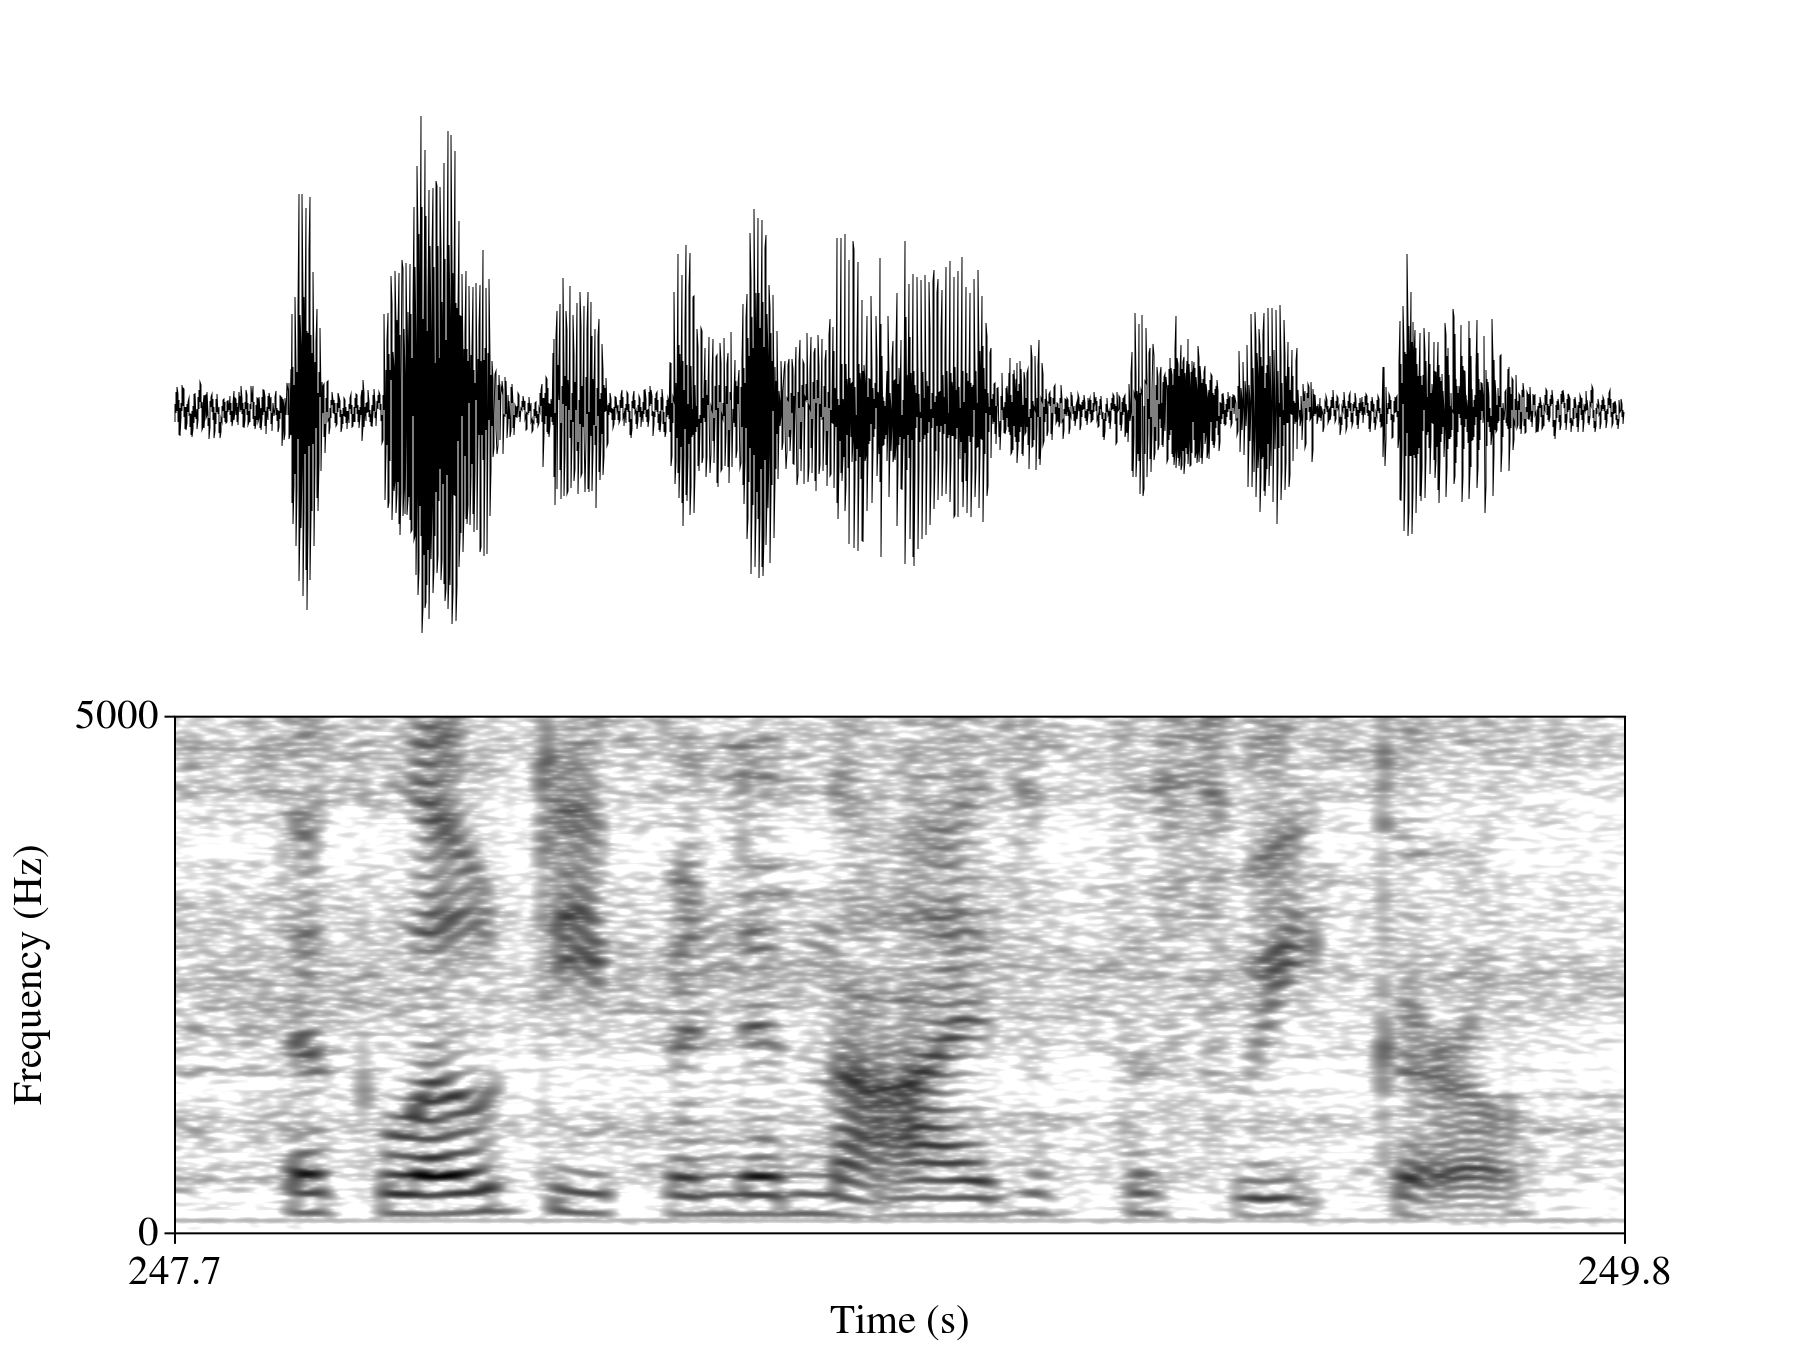
\includegraphics[width=.9\textwidth]{figure/signal-SNR-intro-low.png}
  \caption{\DIFaddFL{A sentence spoken with a high level of background noise, resulting in a }\textit{\DIFaddFL{low}} \DIFaddFL{SNR.}}
  \label{fig:signal-SNR-intro-low}
\end{subfigure}
%DIF > 
\begin{subfigure}{0.75\textwidth}
  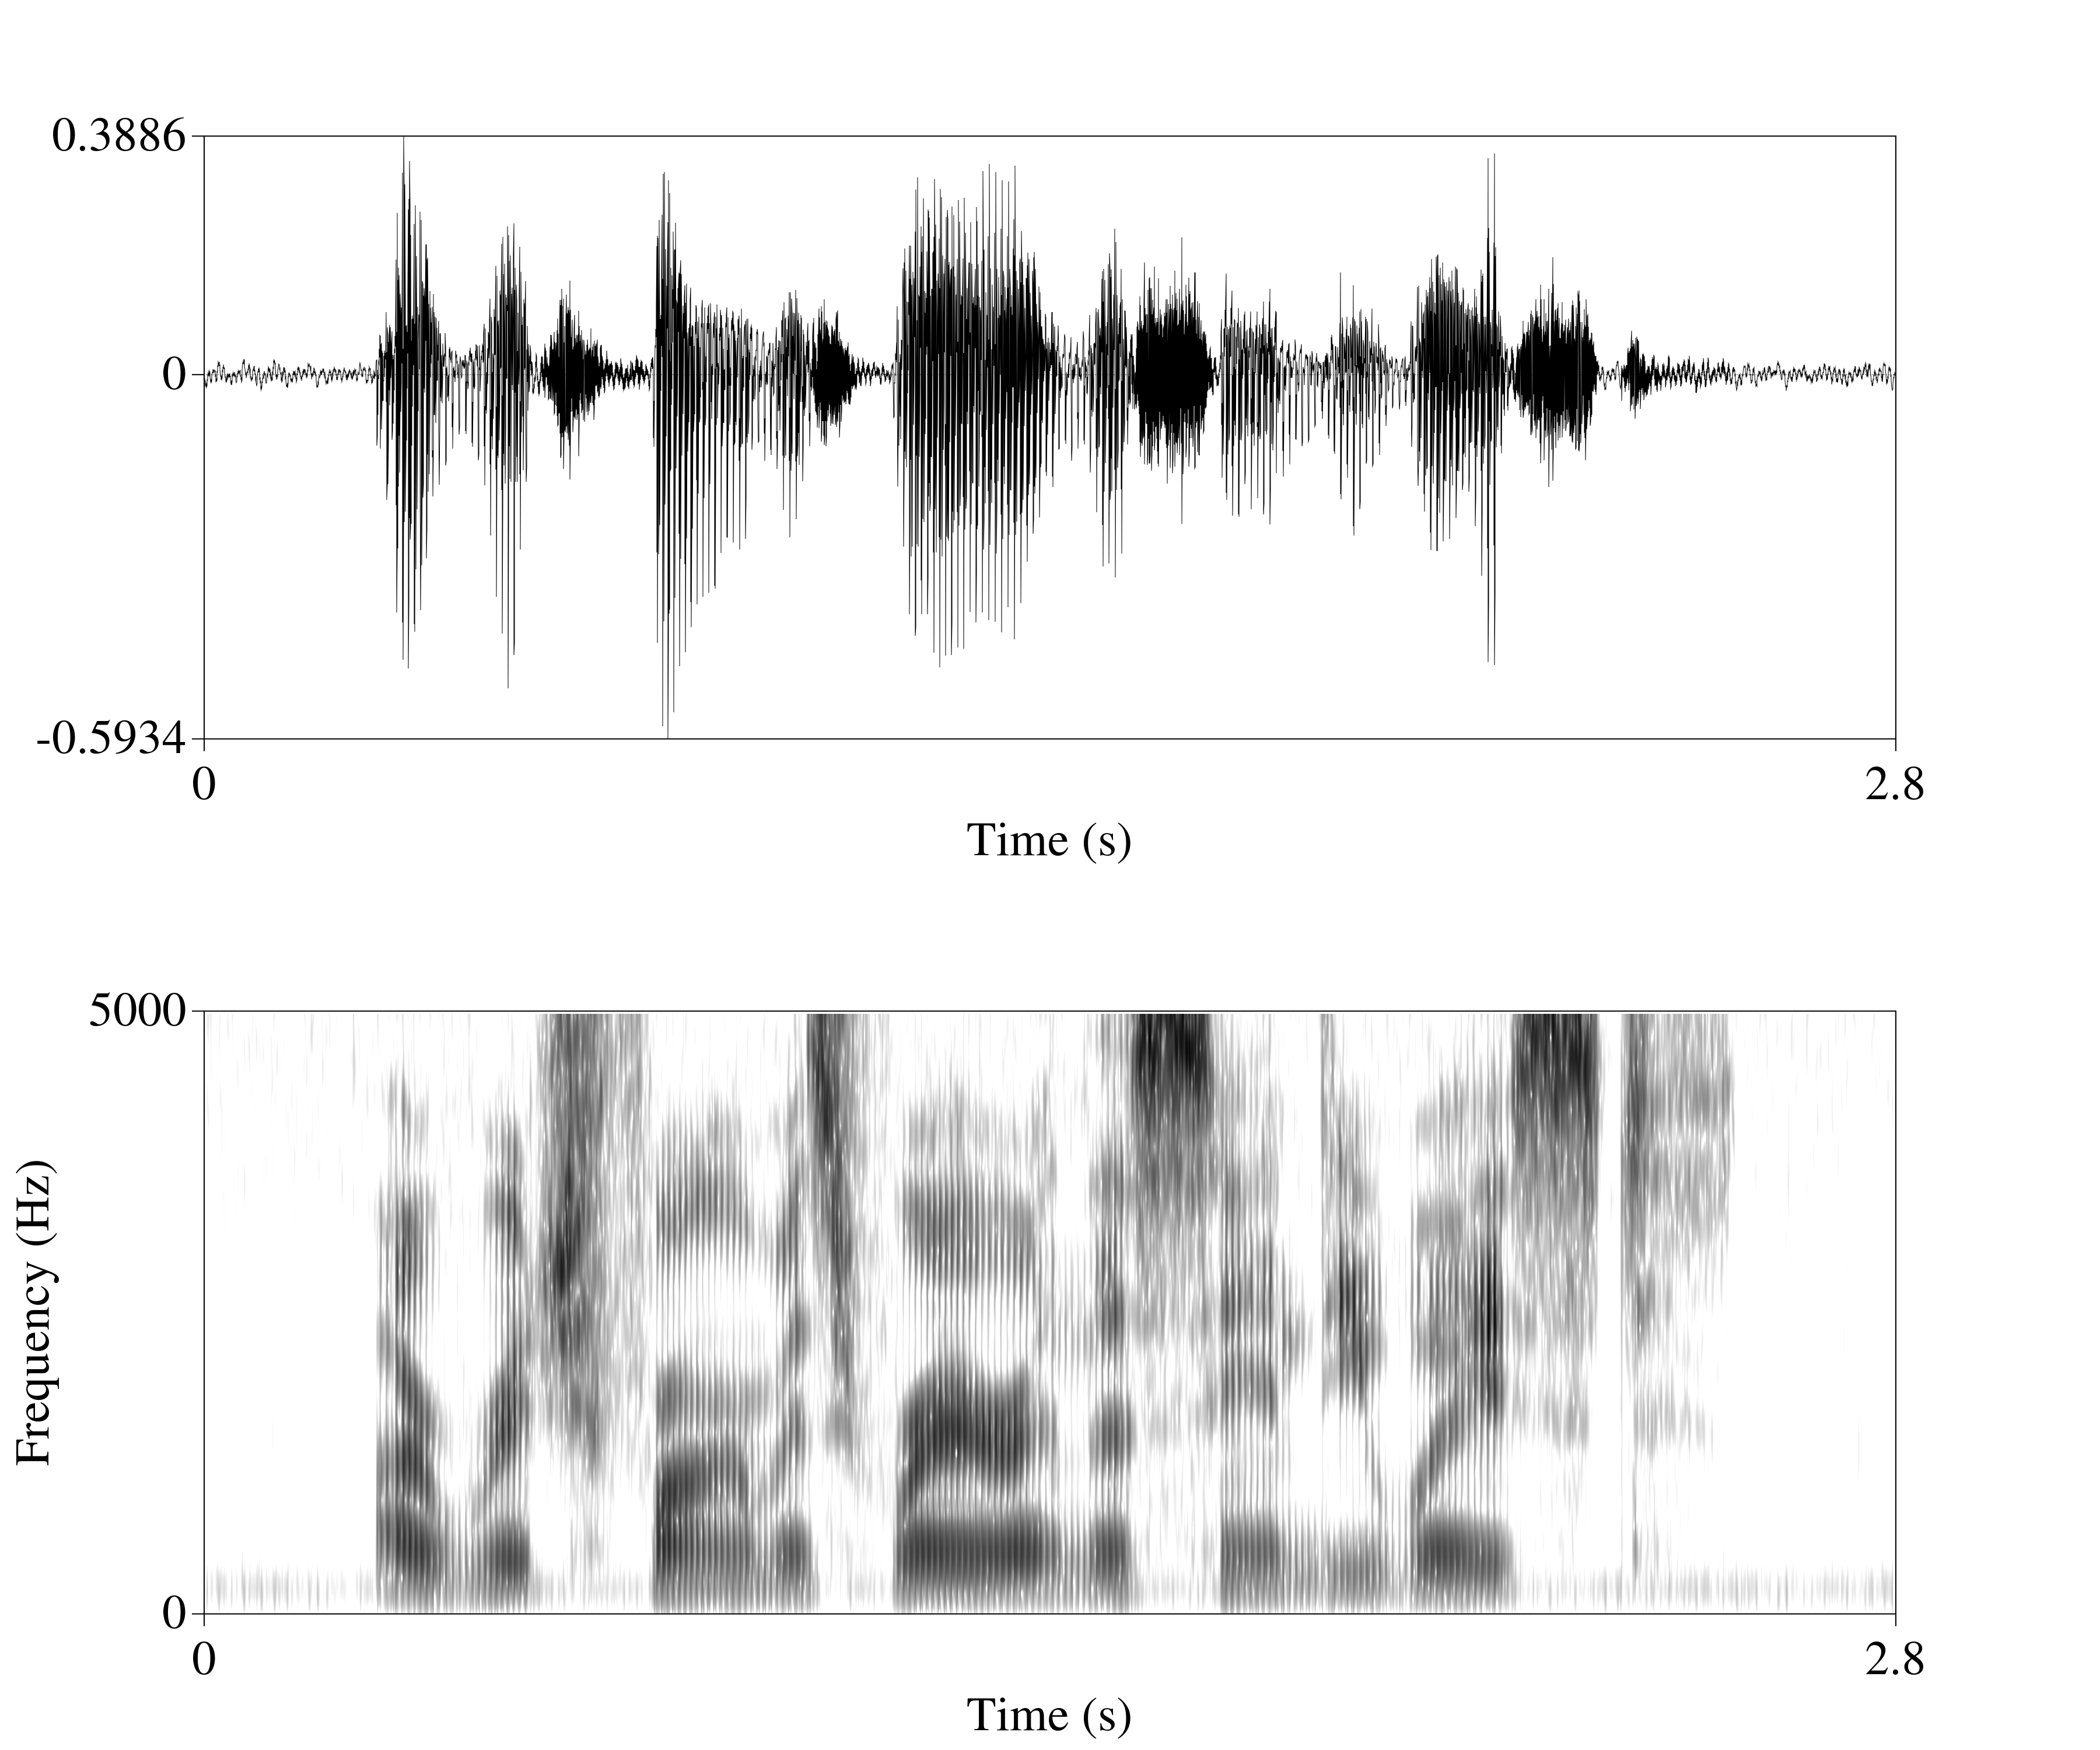
\includegraphics[width=.9\textwidth]{figure/signal-SNR-intro-high.png}
  \caption{\DIFaddFL{A sentence spoken with a low level of background noise, resulting in a }\textit{\DIFaddFL{high}} \DIFaddFL{SNR.}}
  \label{fig:signal-SNR-intro-high}
\end{subfigure}
\caption{\DIFaddFL{Waveforms and spectrograms of the sentence ``The glow deepened in the eyes of the sweet girl.''}}
\label{fig:signal-SNR-intro}
\end{figure}

\DIFaddend This project presents a new approach to the problem.  It proposes that human speech can be recorded in a manner that largely eliminates the noise before it reaches the microphone recording the signal.  The microphone would be placed inside the ear canal of the speaker and would record speech as it is passed through the bone and tissue of the speaker's head.  The signal is expected to be distorted by passage through the head, but the speech in the signal is expected to be recoverable.

Section \ref{ch1:background} below describes the basic acoustics of sound.  This is intended to be a general background to acoustics and interfering sound waves, leading up to a brief overview of sound in noise. Chapter \ref{chapter2} discusses the collection of ear-recorded speech, Chapter \ref{chapter3} describes a human speech perception experiment using ear-recorded speech, and Chapter \ref{chapter4} outlines an experiment testing the ability of an automatic speech recognition system to accurately recognize ear-recorded speech.  At the end of this chapter, Section \ref{ch1:diss-overview} gives a more detailed overview of the rest of the dissertation.

\section{Background}\label{ch1:background}

Sound itself, along with the ability to perceive it, is a remarkable phenomenon.  Put simply, `sound' is the fluctuation of pressure in neighboring groups of particles over time. Most frequently sound is discussed in terms of the fluctuation of air pressure, because, as humans, we primarily receive sound into our ear canals through the medium of air, but sound can also travel through media of liquids and solids, or pass through any combination of the three.

There are primarily three components to sound: amplitude, frequency, and phase, which can be seen in Figure \ref{fig:basic-sound-wave}.  In a simple sound wave, the amplitude of sound corresponds to the peak intensity of the high pressure (and the lowest pressure) portions of a sound wave (cf. Fig. \ref{fig:basic-sound-amplitude}).  The frequency corresponds to the rate at which the high and low pressure portions of the signal fluctuate between one another (cf. Fig. \ref{fig:basic-sound-frequency}).  The phase of a wave is the location of the pressure level (relative to atmospheric pressure) in time (cf. Fig. \ref{fig:basic-sound-phase}).   

\begin{figure}[h!]
\begin{subfigure}{0.5\textwidth}
  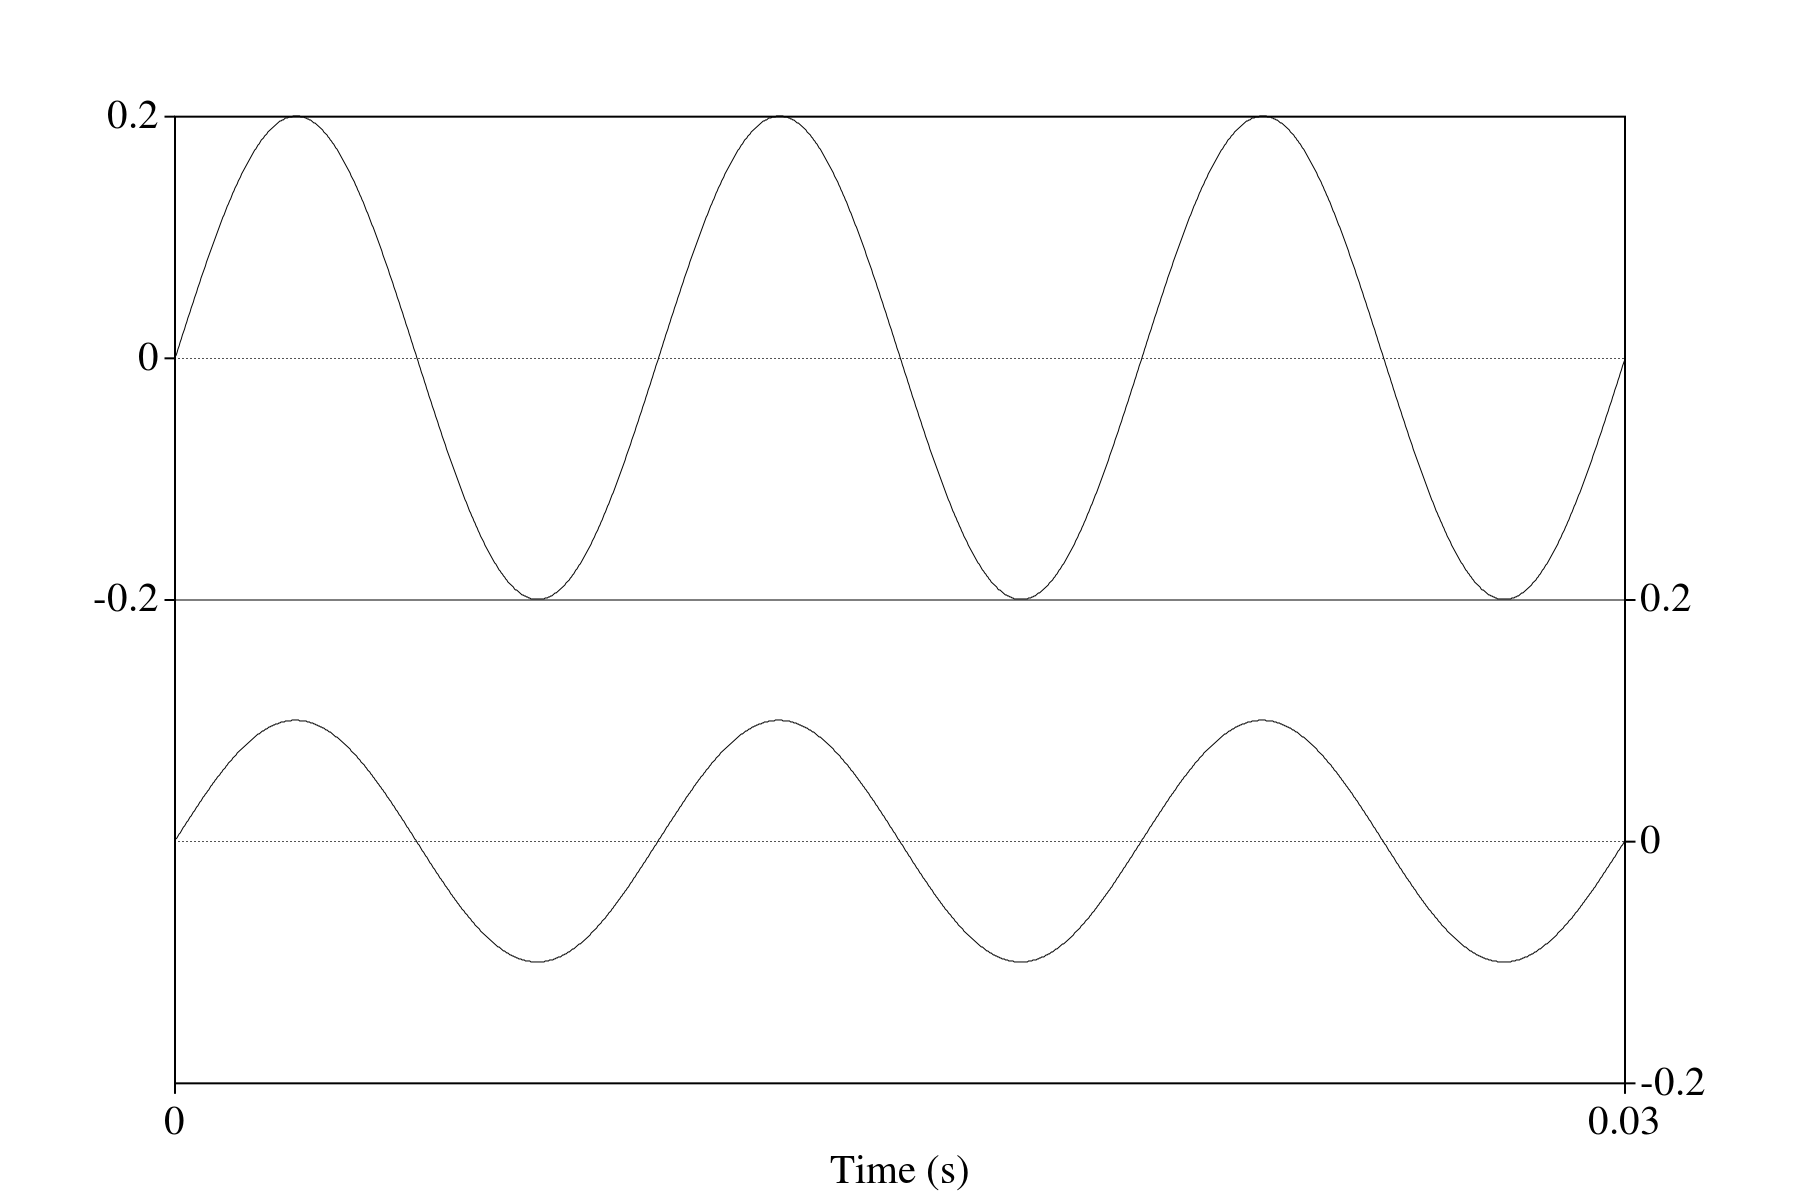
\includegraphics[width=\textwidth]{figure/basic-sound-amplitude.png}
  \caption{Two waveforms showing a difference in amplitude between the two signals.}
  \label{fig:basic-sound-amplitude}
\end{subfigure}
\qquad
\begin{subfigure}{0.5\textwidth}
  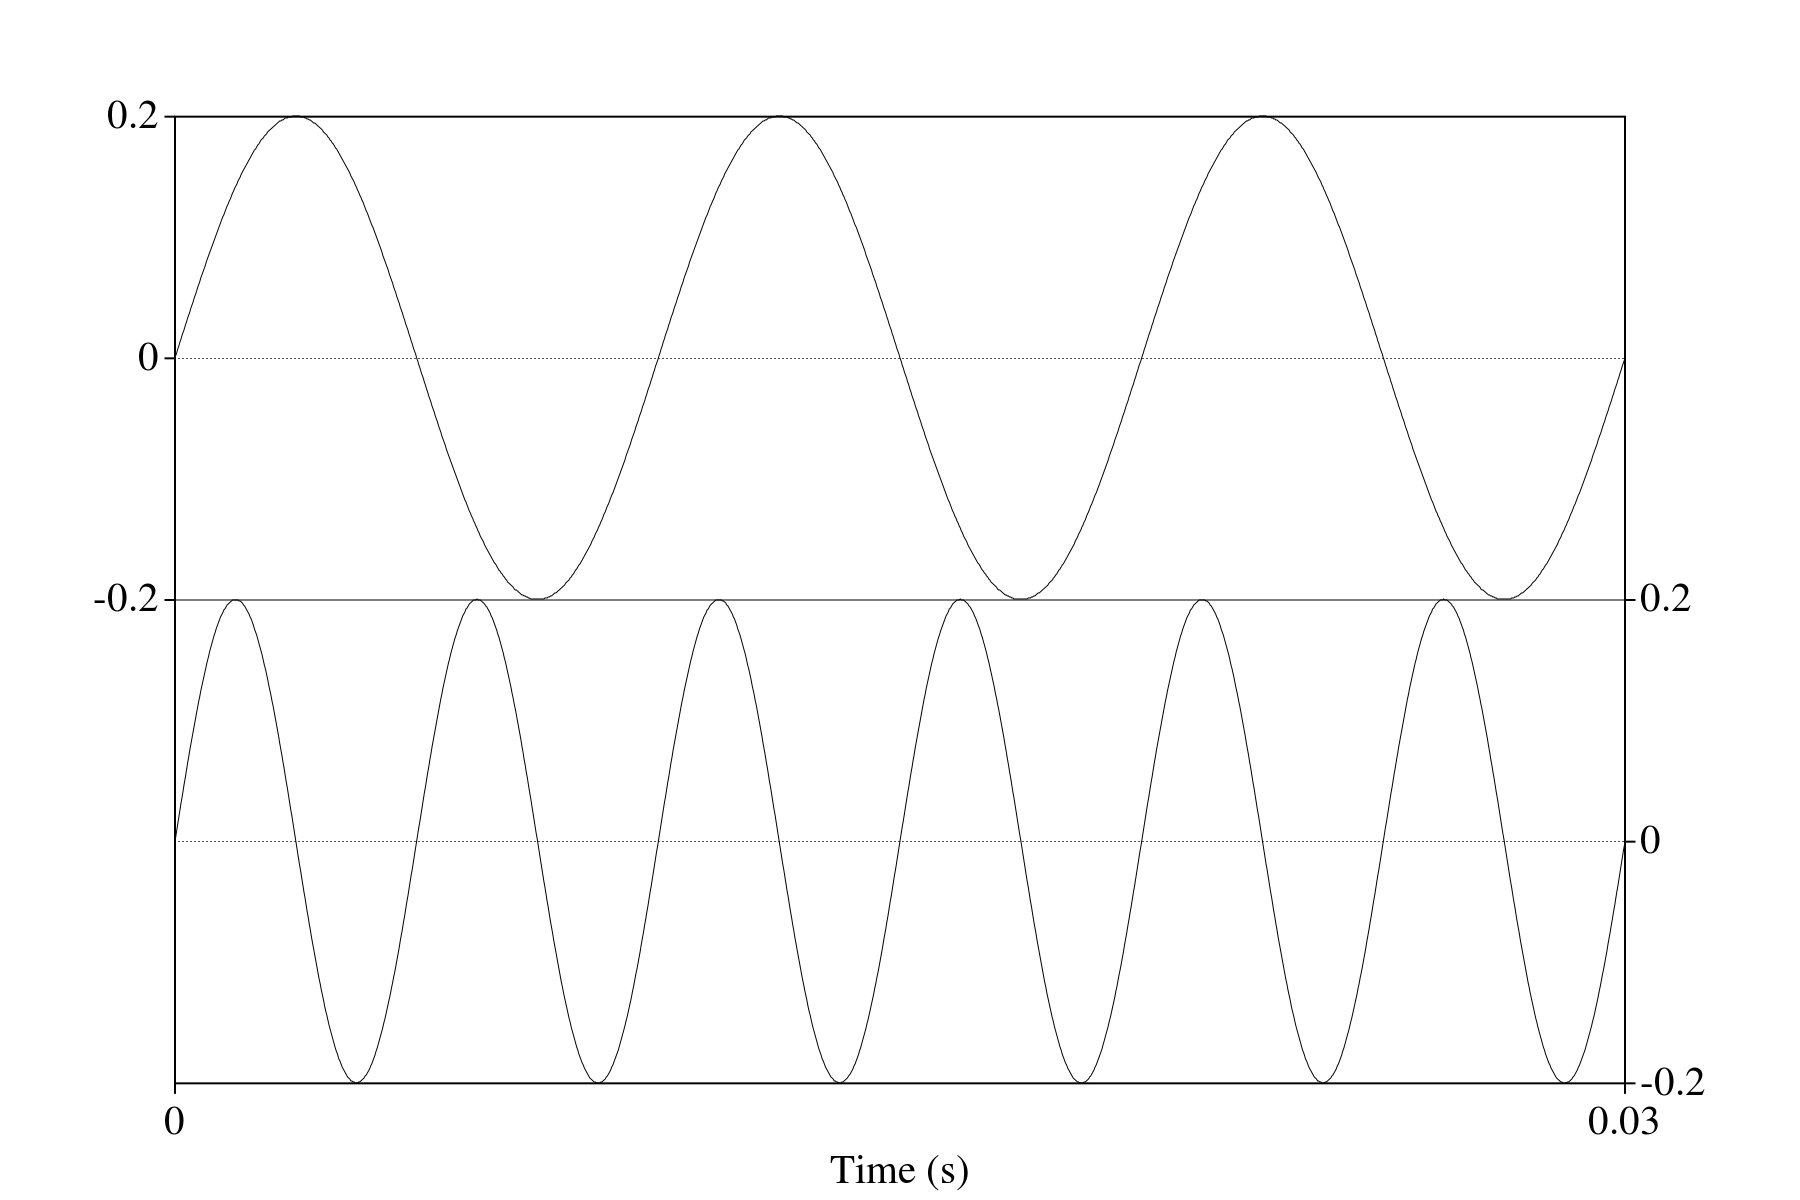
\includegraphics[width=\textwidth]{figure/basic-sound-frequency.png}
  \caption{Two waveforms showing a difference in frequency between the two signals.}
  \label{fig:basic-sound-frequency}
\end{subfigure}
%
\\[2ex]
\begin{center}
\begin{subfigure}{0.5\textwidth}
  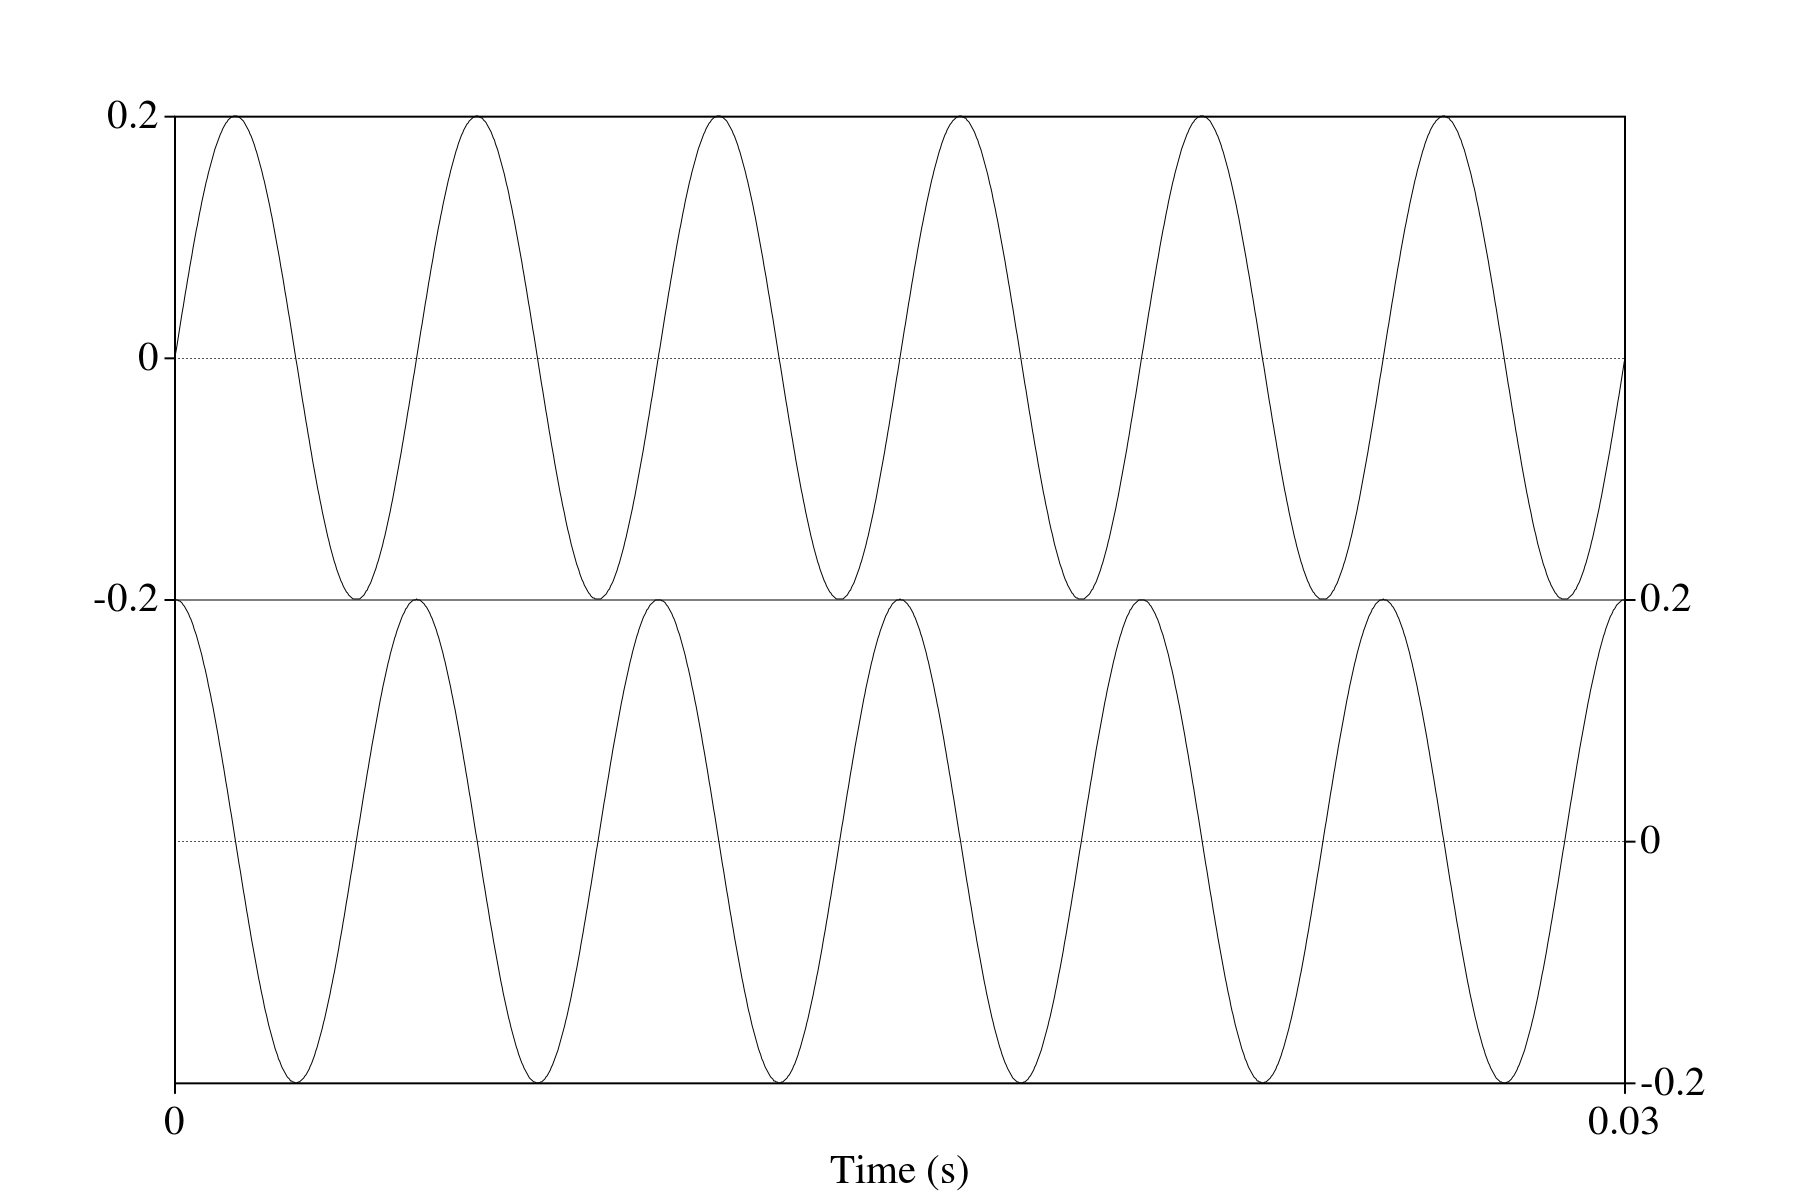
\includegraphics[width=\textwidth]{figure/basic-sound-phase.png}
  \caption{Two waveforms showing a difference in phase between the two signals.}
  \label{fig:basic-sound-phase}
\end{subfigure}
\end{center}
\caption{Waveforms demonstrating difference in amplitude, frequency, and phase.}
\label{fig:basic-sound-wave}
\end{figure}

This latter characteristic - phase, while important when dealing with interacting waves from multiple sources, is often not taken into in speech science due to both its complexity and the fact that phase does not encode any speech information.  The human auditory system primarily makes use of the other two characteristics of sound - amplitude and frequency.

\subsection{Overview of Anatomy and Physiology of the Peripheral Auditory System}

Prior to discussing the acoustic structure of speech, it is important to become familiar with the basic peripheral auditory system.  The peripheral auditory system is generally grouped into three primary categories, the outer ear, the middle ear, and the inner ear (cf. Figure \ref{fig:ear-anatomy}).  The outer ear includes the pinna, the ear canal tube, and the tympanic membrane (ie. the eardrum).  Air-transmitted sound vibrations, ie. pressure fluctuations, enter the ear canal through the opening at the pinna.  These then travel along the canal to vibrate the tympanic membrane, which passes the energy to the middle ear.  The middle ear includes the ossicles within the middle ear cavity.  The ossicles are a chain of three very small bones leading from the tympanic membrane to the cochlea. The external sound vibrations hit the tympanic membrane, are passed along the ossicle chain, which then sends these vibrations to the inner ear (\cite{rosen:91}).

\begin{figure}[h]
\centering
  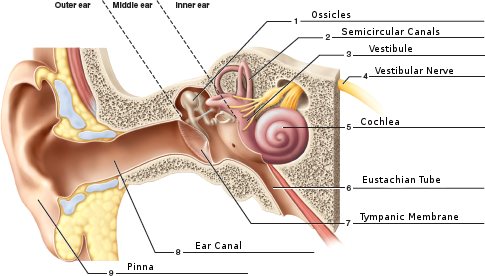
\includegraphics{figure/ear_anatomy.png}
  \caption{A diagram of the peripheral auditory system, including the outer ear, middle ear, and inner ear, up to the auditory nerve. (Image from \cite{martin:12})}
  \label{fig:ear-anatomy}
\end{figure}

The inner ear is composed of the cochlea, the semicircular canals (and vestibule), and the auditory and vestibular nerves.  The semicircular canals, vestibule, and vestibular nerve don't play a part in audition (their primary function regards balance sensitivity).  The cochlea, a hard `shell' filled with fluid receives the vibrations passed along through the middle ear ossicles.\footnote{The peripheral auditory system uses gas, solid, and liquid media to transmit acoustic vibrations.}  The vibrations are passed into the fluid cochlea and travel along the length of the cochlea, transmitting acoustic energy to cells that are able to detect the amplitude of the vibrations.  Depending on the location of a cell along the length of the cochlea, it will pick up a different frequency of sound.  The auditory nerve carries electrical impulses from these cells into the auditory cortex of the brain. 

Of interest to this present study is the relatively simple outer ear.  Typically, as described above, vibrations from the air will enter the ear canal through the opening at the pinna. Frequently, these vibrations take the form of human speech.

%However, vibrations from one's own speech are also transmitted via the bone, cartilage, and tissue of the head.  Regardless of source, sound vibrations entering into the ear canal will be altered by the shape of the ear canal, described more below.


\subsection{Acoustic Structure of Human Speech}

The structure of human speech draws from a collection of individual sounds (phonemes) that are strung together, encoding words, sentences, and more abstractly, meaning.  Each human language uses a subset of all possible phonemes.  Each phoneme is either considered `voiced' or `unvoiced'.  The acoustic properties of sounds in these two categories differ greatly.

Voiced speech is composed of narrow bands of acoustic energy, called harmonics, located along a frequency spectrum (cf. fig \ref{fig:spctrm5k}).  In this sense, speech is considered a `complex' sound, because it is composed of multiple, simultaneous frequencies.
%
\begin{wrapfigure}{l}{0.5\textwidth}
\centering
  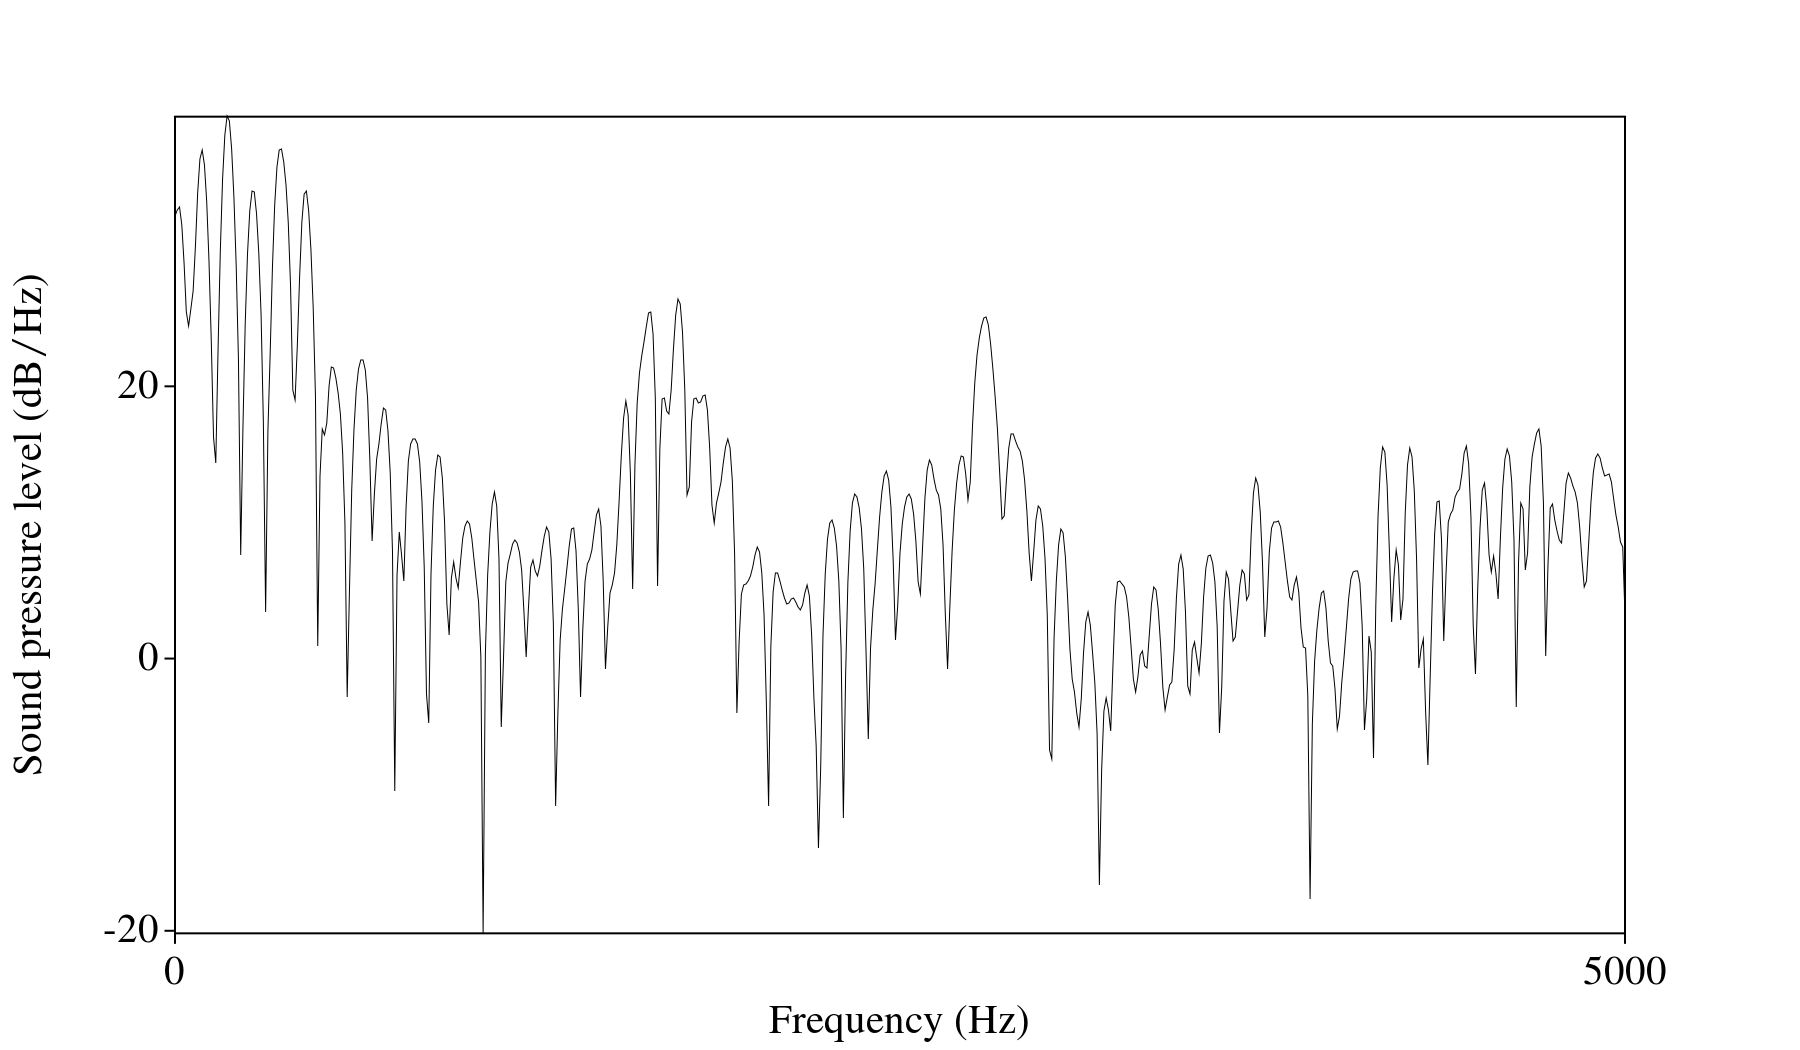
\includegraphics[width=0.5\textwidth]{figure/spctrm5k.png}
  \caption{Spectrum of the middle of an /I/ vowel.  Each `spike' is a separate narrow band of frequency, called a harmonic.}
  \label{fig:spctrm5k}
\end{wrapfigure}
%
Certain harmonics will be dampened by the vocal tract, leaving others relatively unfiltered.  A group of neighboring harmonics containing more energy than other harmonics are called formants.  The location, shape, and transition over time of these formants (among other more minor features) are what encodes speech information for voiced sounds.  This can be easily visualized in a spectrogram (cf. Fig. \ref{fig:spctgrm_citizen}).

\begin{figure}[h!]
\begin{subfigure}{0.95\textwidth}
  \centering
  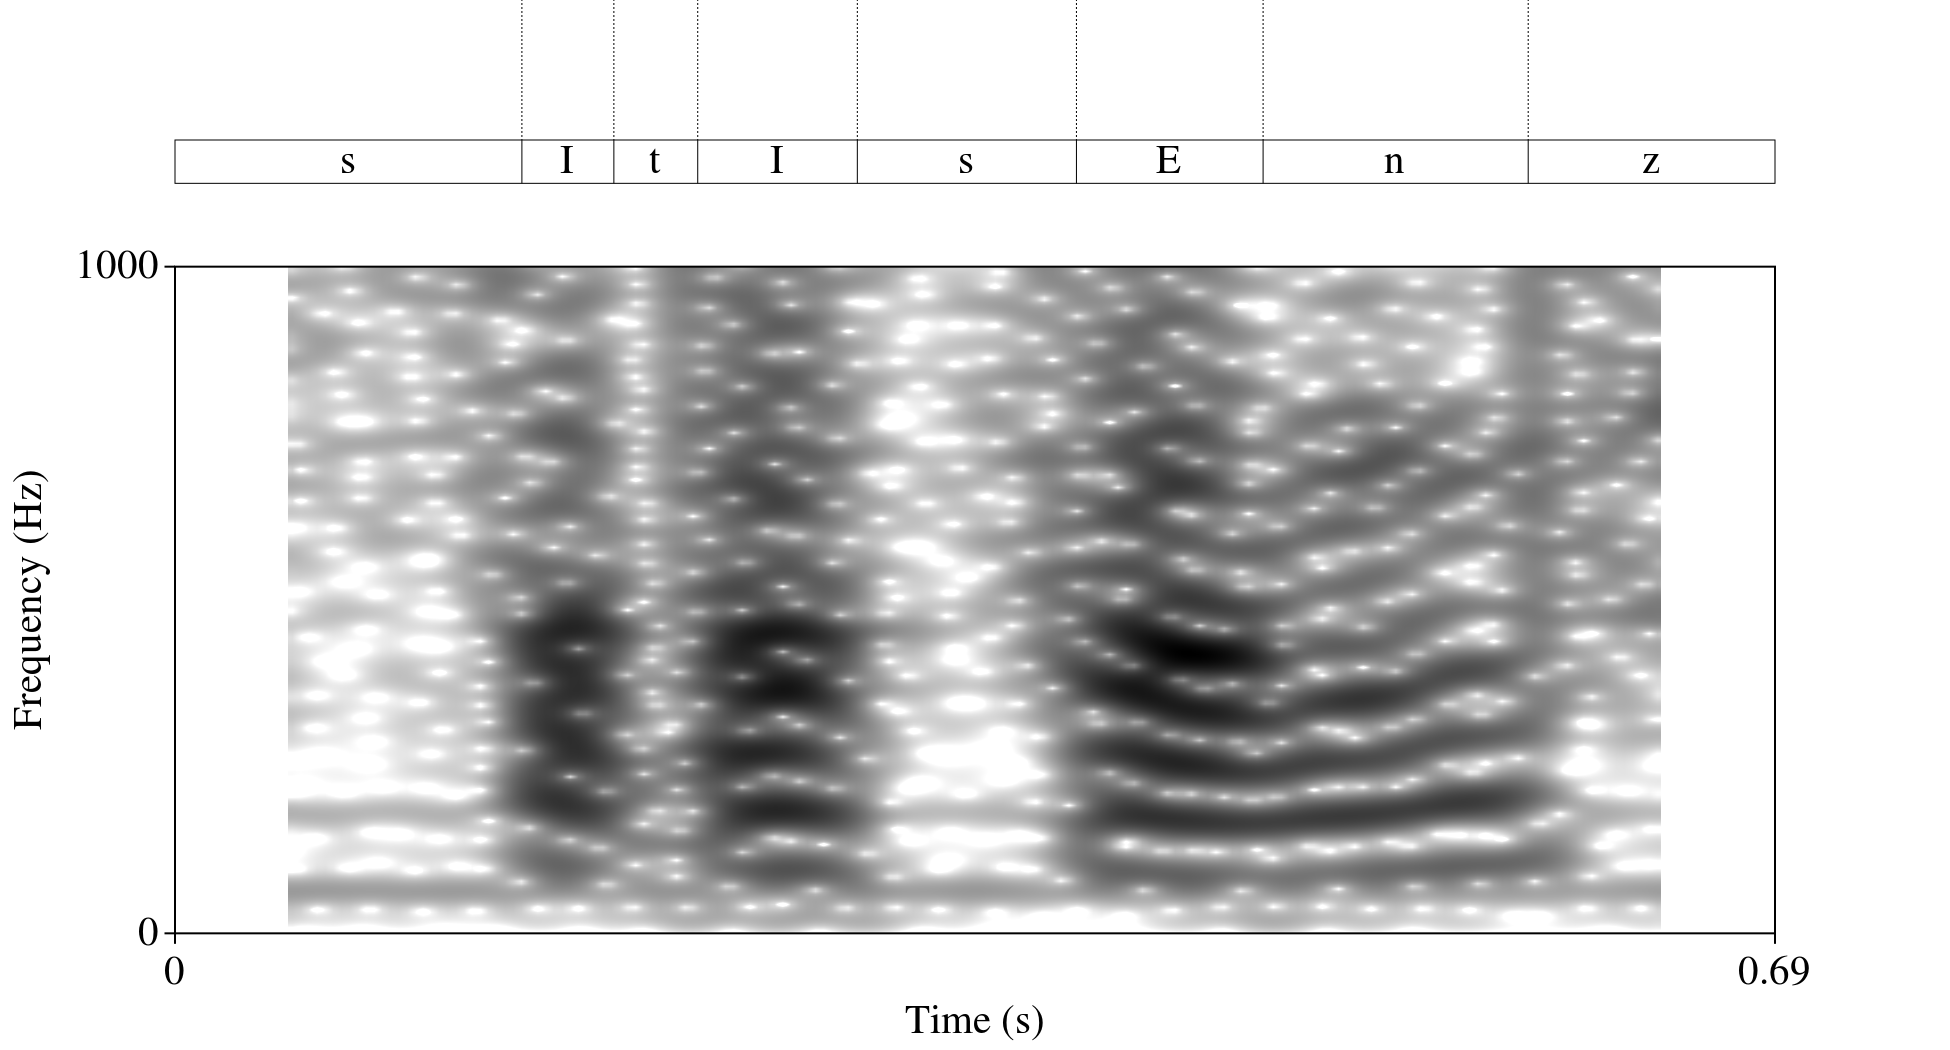
\includegraphics[width=0.95\textwidth]{figure/spctgrm1k.png}
  \caption{Zoomed to the 0-1kHz range for better visualization of harmonics.}
  \label{fig:spctgrm_citizen_1k}
\end{subfigure}%
\hfill
\begin{subfigure}{0.95\textwidth}
  \centering
  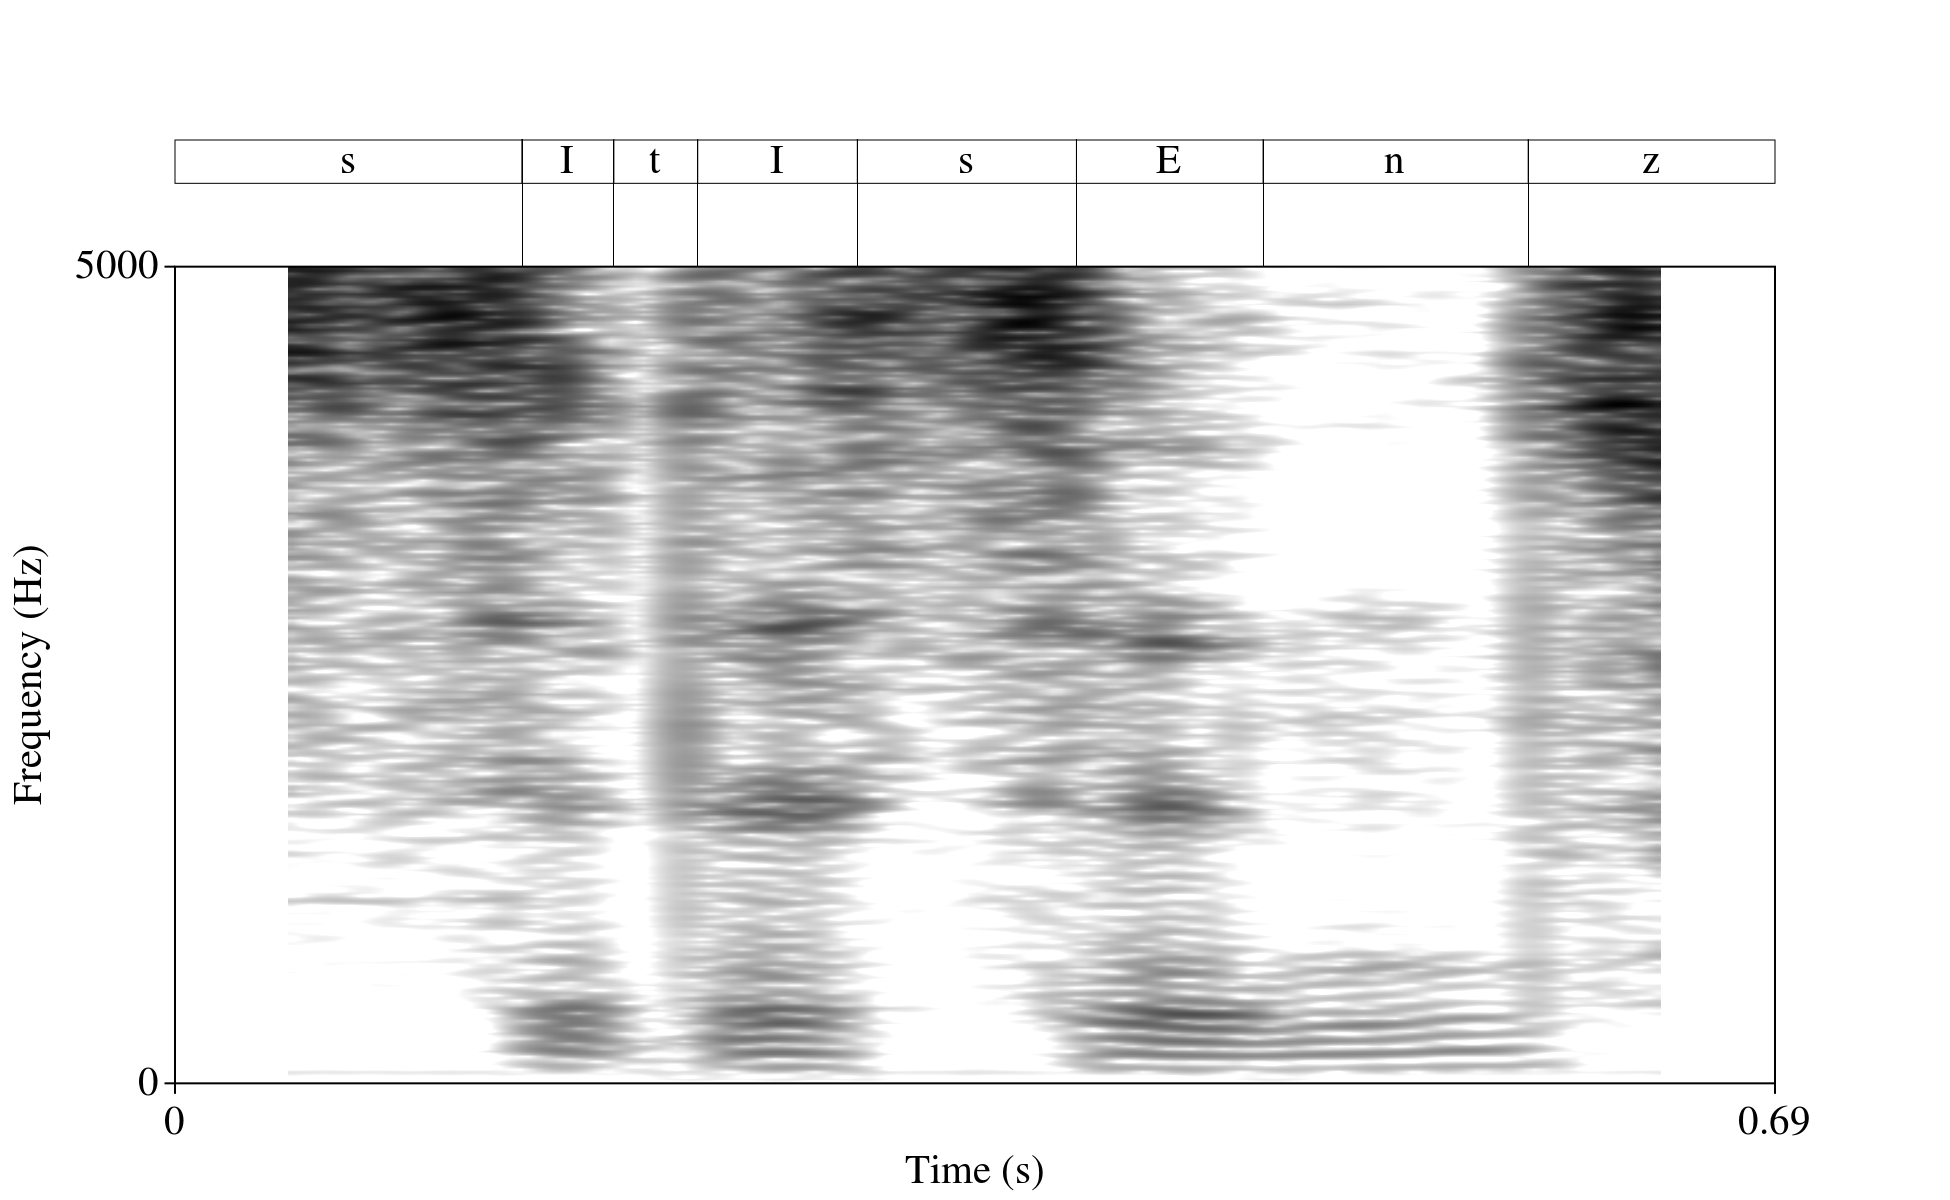
\includegraphics[width=0.95\textwidth]{figure/spctgrm5k.png}
  \caption{Zoomed to a more standard 0-5kHz range.}
  \label{fig:spctgrm_citizen_5k}
\end{subfigure}
\caption{Narrow-band spectrogram of the word `citizens' with phonetic transcription above.  Frequency is on the y-axis, time is on the x-axis, and amplitude is shown in grayscale on the graph; the darker an area of the graph, the greater the amplitude.}
\label{fig:spctgrm_citizen}
\end{figure}

For unvoiced speech, the information used to recognize and categorize the speech sound is likely found in either the turbulent frication generally centered in higher frequencies (cf. Fig. \ref{fig:spctgrm_s}, although some of the information can be found in lower frequencies), or found in the voiced information in the transitions into and out of the sound (\cite{halle:57,lindblom:63,stevens:78,willi:17}).  Generally, most speech information used by the human auditory system can be found in frequencies below 5.0-8.0 kHz.
%
\begin{wrapfigure}{l}{0.5\textwidth}
\centering
  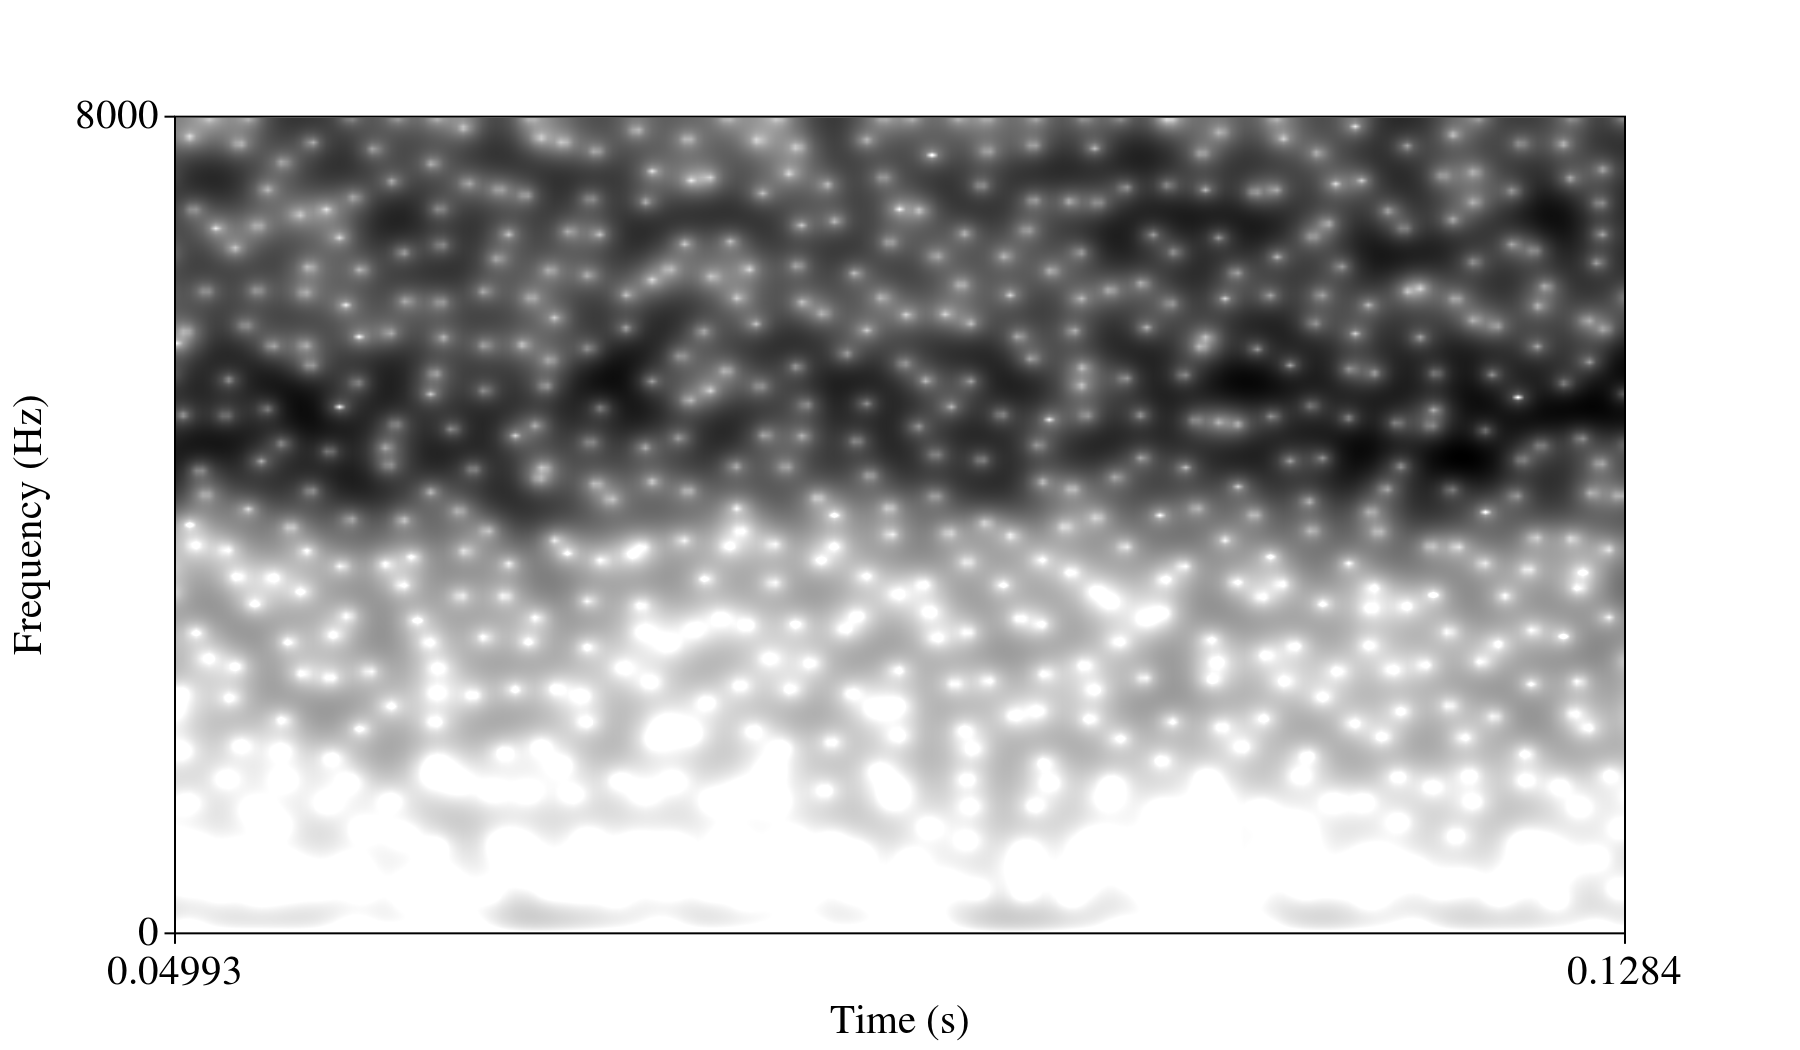
\includegraphics[width=0.5\textwidth]{figure/spctgrm_s.png}
  \caption{Spectrum of the initial /s/ in `citizens'. Zoomed to range of 0-8kHz for visualization of high frequency energy.}
  \label{fig:spctgrm_s}
\end{wrapfigure}

The human auditory system has the remarkable ability to (a) identify these sounds, which often only last from tens to a few hundreds of milliseconds in duration, (b) partition the stream of sounds into their respective words, and (c) string the words together into a sentence and pull meaning from it - all in real time.  Nevertheless there are occasionally recognition errors, which can occur anywhere along this auditory chain.  The `lowest' level in this chain that errors occur is the recognition and identification of sounds.  There are a host of reasons why this might occur, yet this focuses on additive noise interfering with the speech signal and signal distortion via passage of speech through a speaker's head.

\subsection{Acoustics of Multiple Signals}

As previously mentioned, we as humans use the amplitude and frequency of pressure fluctuations to perceive sound. When sound travels through a medium from source \textit{A}, there is nothing that prevents these pressure fluctuations of source \textit{A} from acoustically mixing with the pressure fluctuations originating from source \textit{B}.  For example, in Figure \ref{fig:sound-wave-addition} source \textit{A} produces a simple wave with a frequency of 100 Hz.  Source \textit{B} produces a simple wave with a frequency of 200 Hz.  If the waves from the two sources reach each other and overlap, a single wave results that looks like that in Figure \ref{fig:sound-wave-addition-combined}.  This sound wave now has two components - a tone at 100 Hz and a tone at 200 Hz.

\begin{figure}[h!]
\begin{subfigure}{0.5\textwidth}
  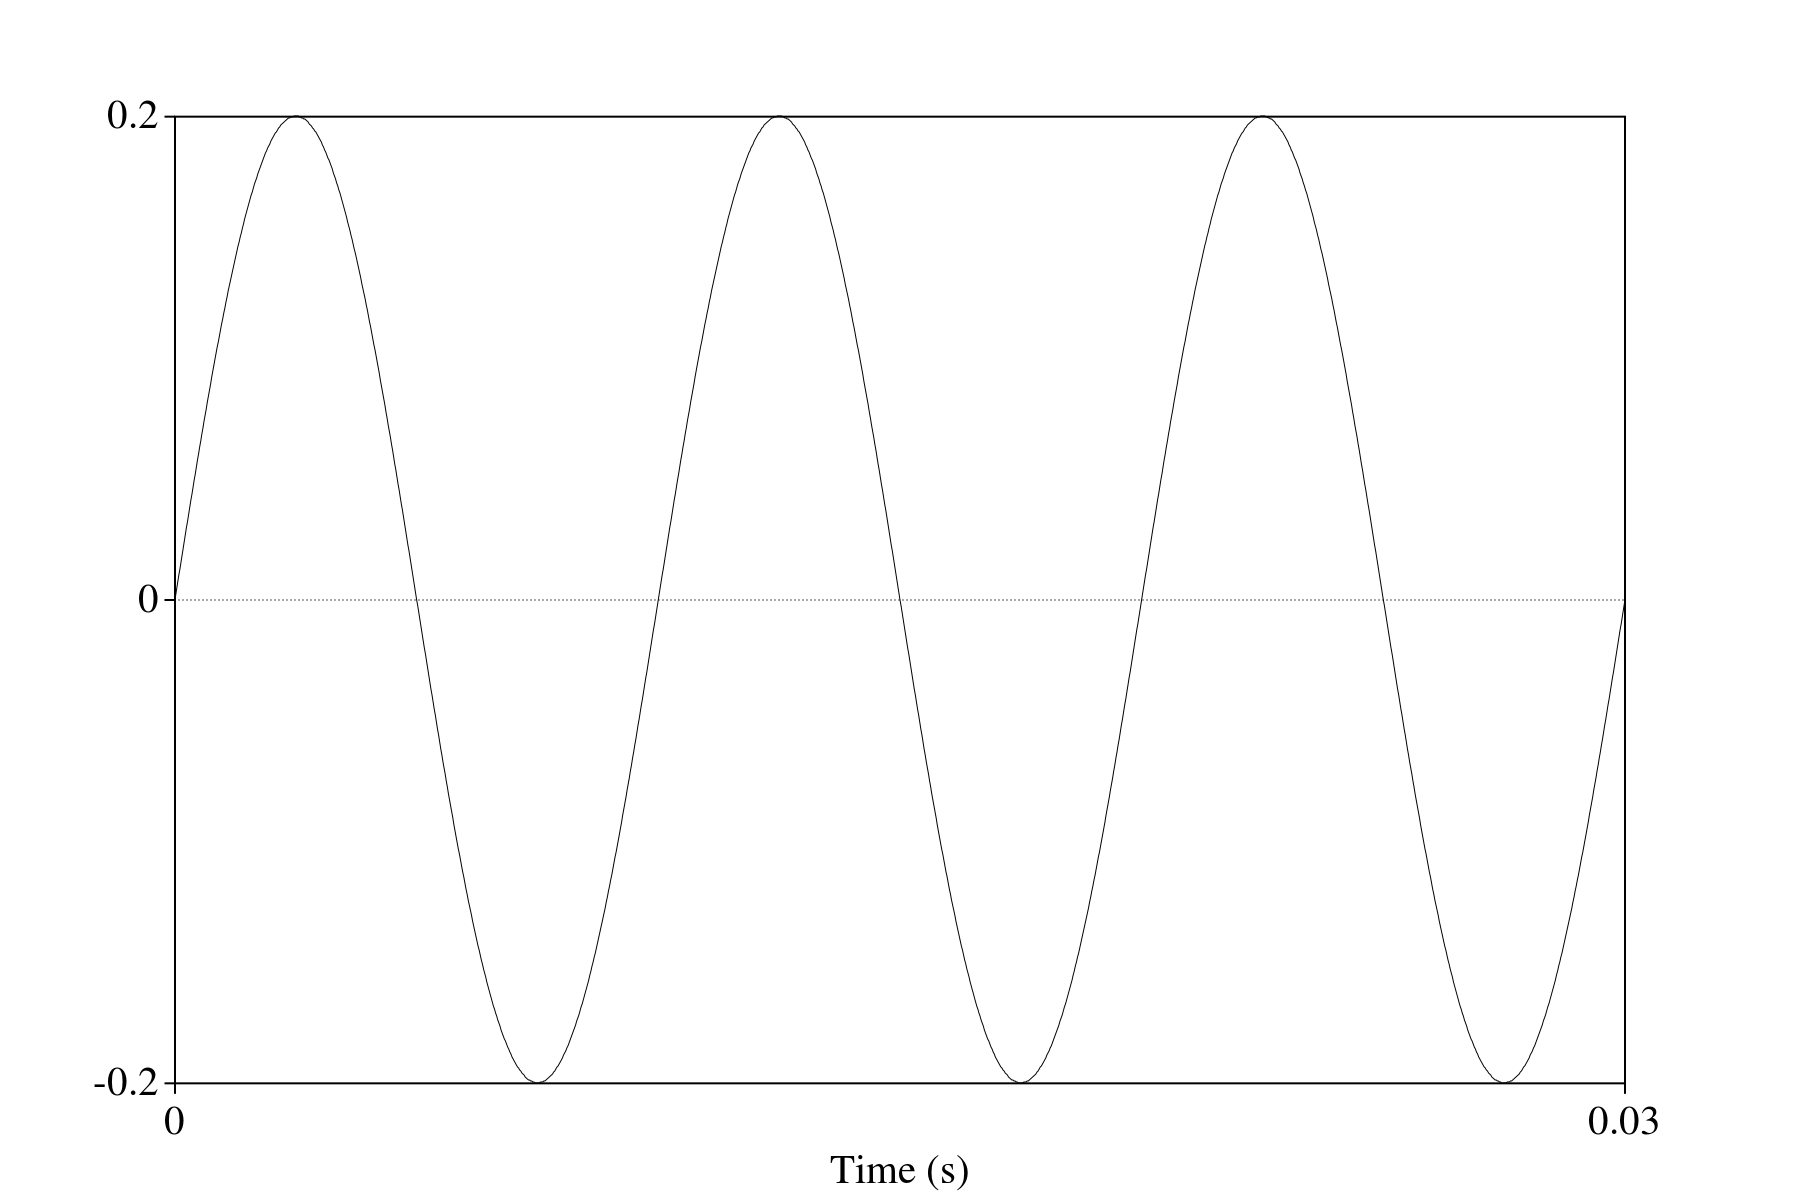
\includegraphics[width=\textwidth]{figure/basic-sound-wave.png}
  \caption{A basic sound wave from source \textit{A} at a frequency of 100 Hz.}
  \label{fig:sound-wave-A}
\end{subfigure}
\qquad
\begin{subfigure}{0.5\textwidth}
  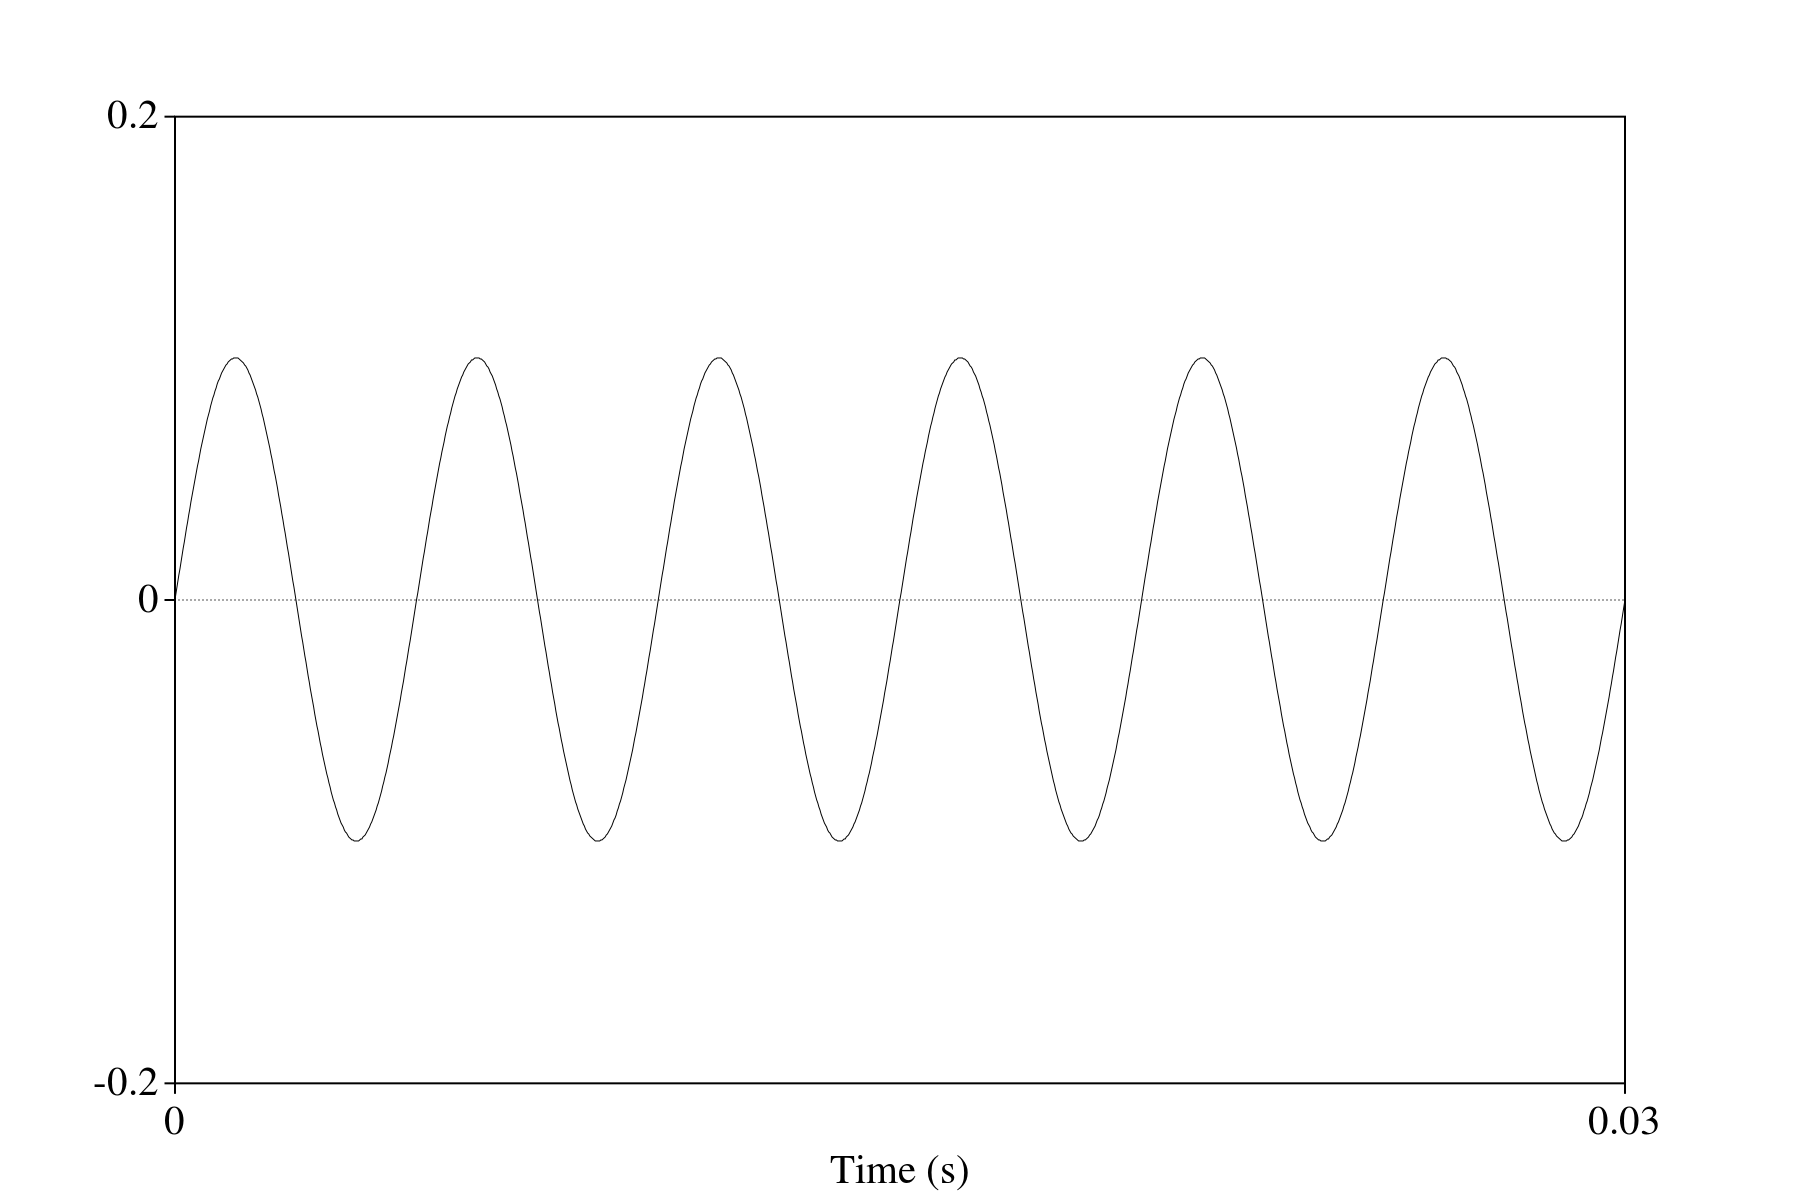
\includegraphics[width=\textwidth]{figure/sound-wave-addition-200hz.png}
  \caption{A basic sound wave from source \textit{B} at a frequency of 200 Hz, with half the amplitude of the simple sound wave from source \textit{A}.}
  \label{fig:sound-wave-B}
\end{subfigure}
%
\\[2ex]
\begin{center}
\begin{subfigure}{0.5\textwidth}
  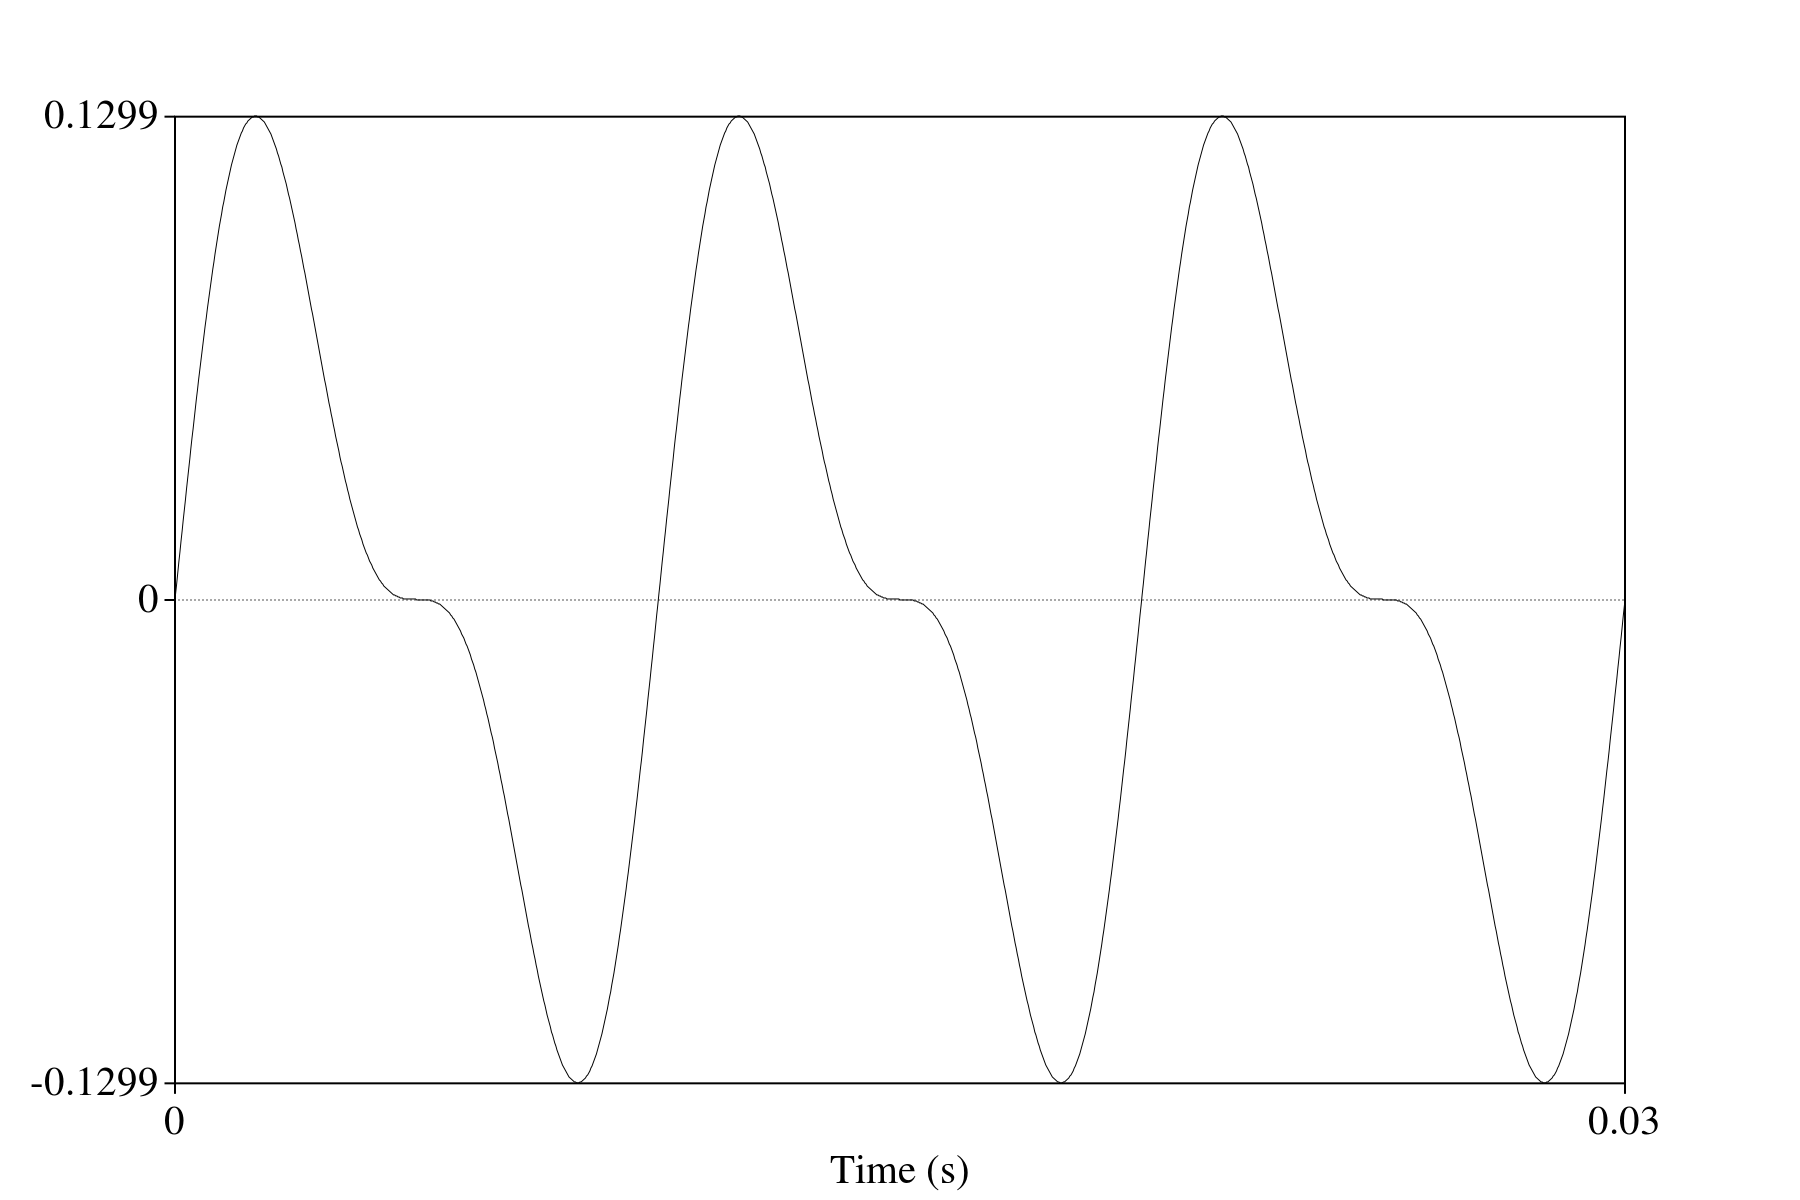
\includegraphics[width=\textwidth]{figure/sound-wave-addition-combined.png}
  \caption{The resulting complex wave from the combination of the wave from source \textit{A} and source \textit{B}.}
  \label{fig:sound-wave-addition-combined}
\end{subfigure}
\end{center}
\caption{Demonstration of the combination of two waves of different frequency and amplitude.}
\label{fig:sound-wave-addition}
\end{figure}

As previously mentioned, phase does not play a significant role in human audition, but can affect a wave resulting from the addition of multiple sound sources.  Say that source \textit{B} produces instead a wave the same frequency and amplitude as the wave from source \textit{A}, but they are completely `out of phase', ie. the pressure value of the waves at any given time is in direct opposition (cf. Figure \ref{fig:wave-out-of-phase}).  If these waves are combined, it results in a complete elimination of sound (cf. Fig. \ref{fig:wave-out-of-phase-added}).

\begin{figure}[h!]
\begin{subfigure}{0.5\textwidth}
  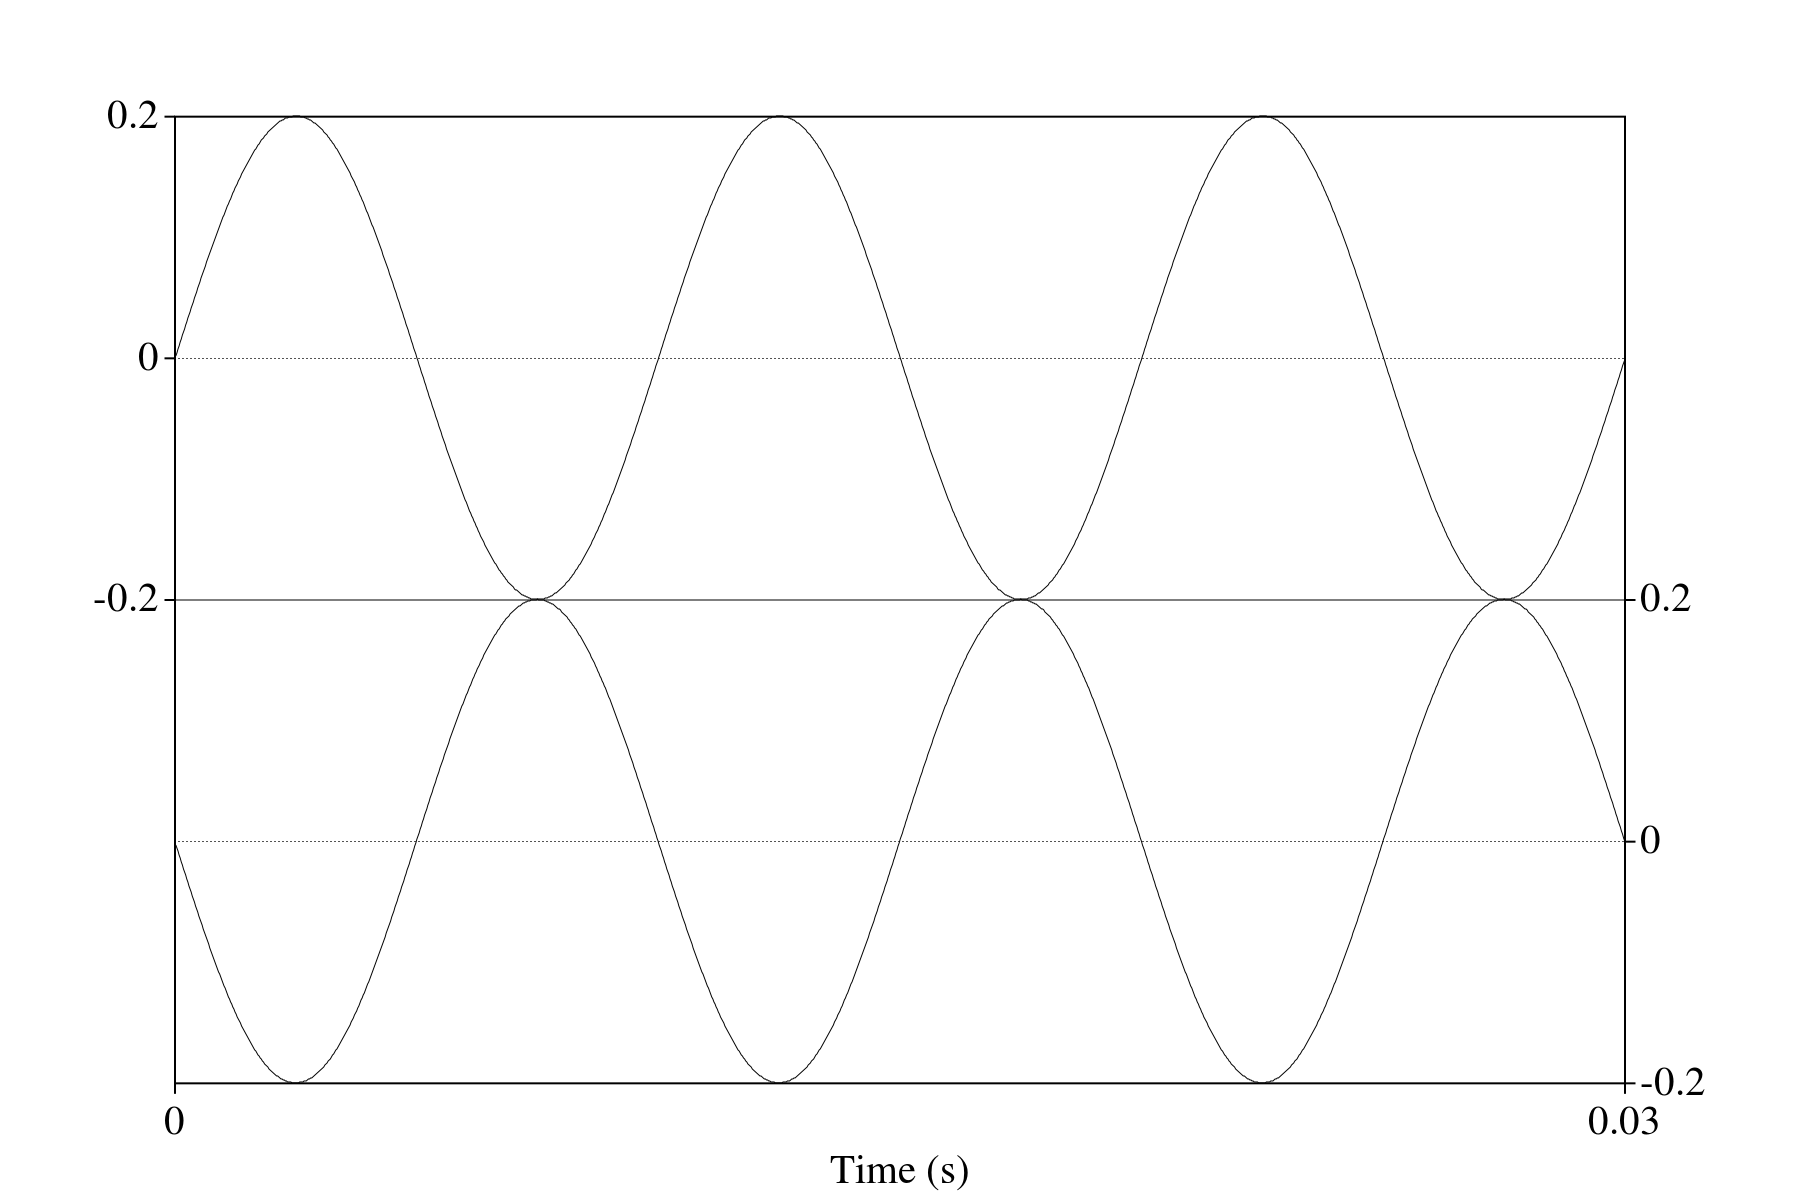
\includegraphics[width=\textwidth]{figure/wave-out-of-phase.png}
  \caption{Two sound waves with frequency of 100 Hz and the same amplitude, completely out of phase.}
  \label{fig:wave-out-of-phase}
\end{subfigure}
\qquad
\begin{subfigure}{0.5\textwidth}
  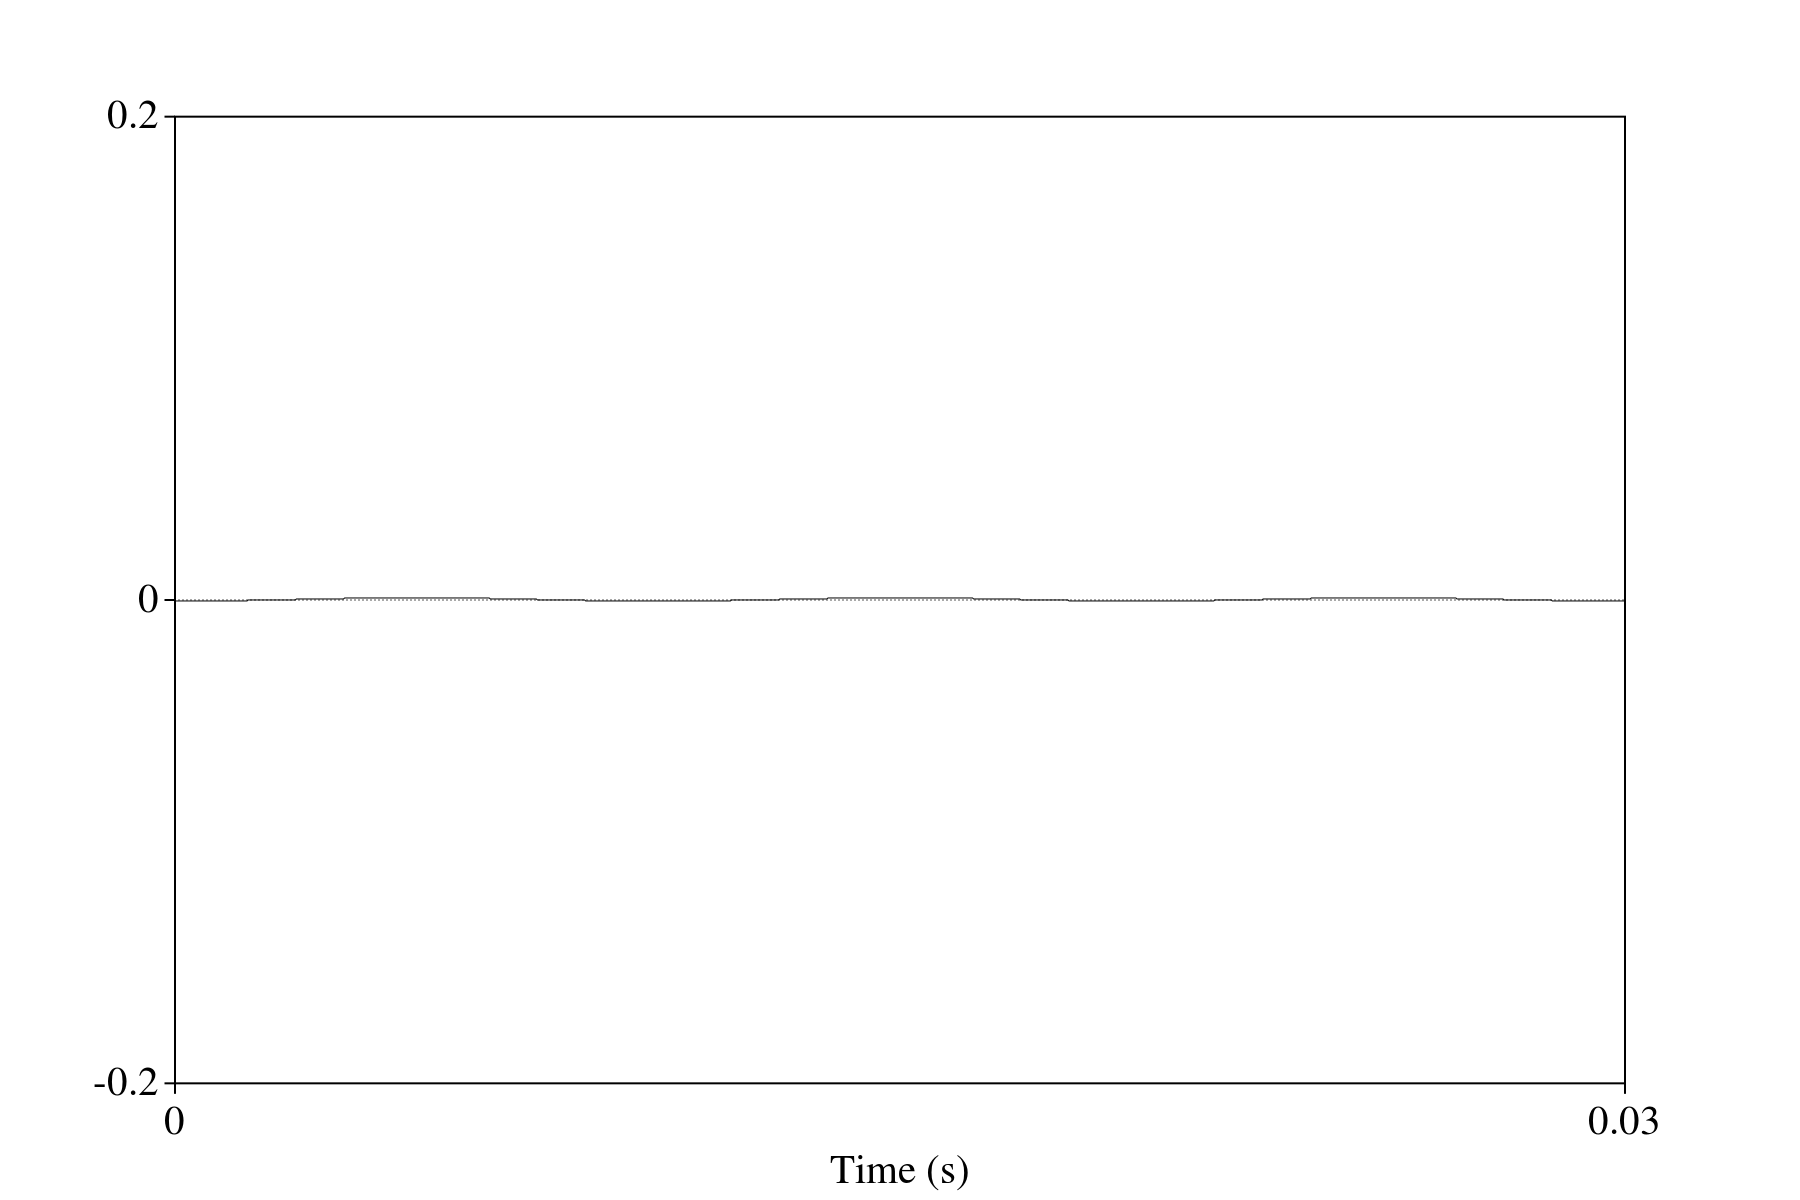
\includegraphics[width=\textwidth]{figure/wave-out-of-phase-added.png}
  \caption{The sound wave resulting from the combination of the two out of phase waves in Fig. \ref{fig:wave-out-of-phase}.}
  \label{fig:wave-out-of-phase-added}
\end{subfigure}
\caption{Demonstration of the combination of two completely out-of-phase waves with the same amplitude and frequency.}
\end{figure}

It is not very often that two waves of the exact same frequency and amplitude, with exactly opposing phase, meet in such a way to completely negate.  However, varying degrees of negation occur frequently due to phase.  For example, if the 100 Hz wave from Figure \ref{fig:sound-wave-addition} were combined with a 200Hz wave with a slightly shifted phase, a different wave would be produced, seen in Figure \ref{fig:sound-combined-shifted-phase}.  

\begin{figure}[h!]
\begin{subfigure}{0.5\textwidth}
  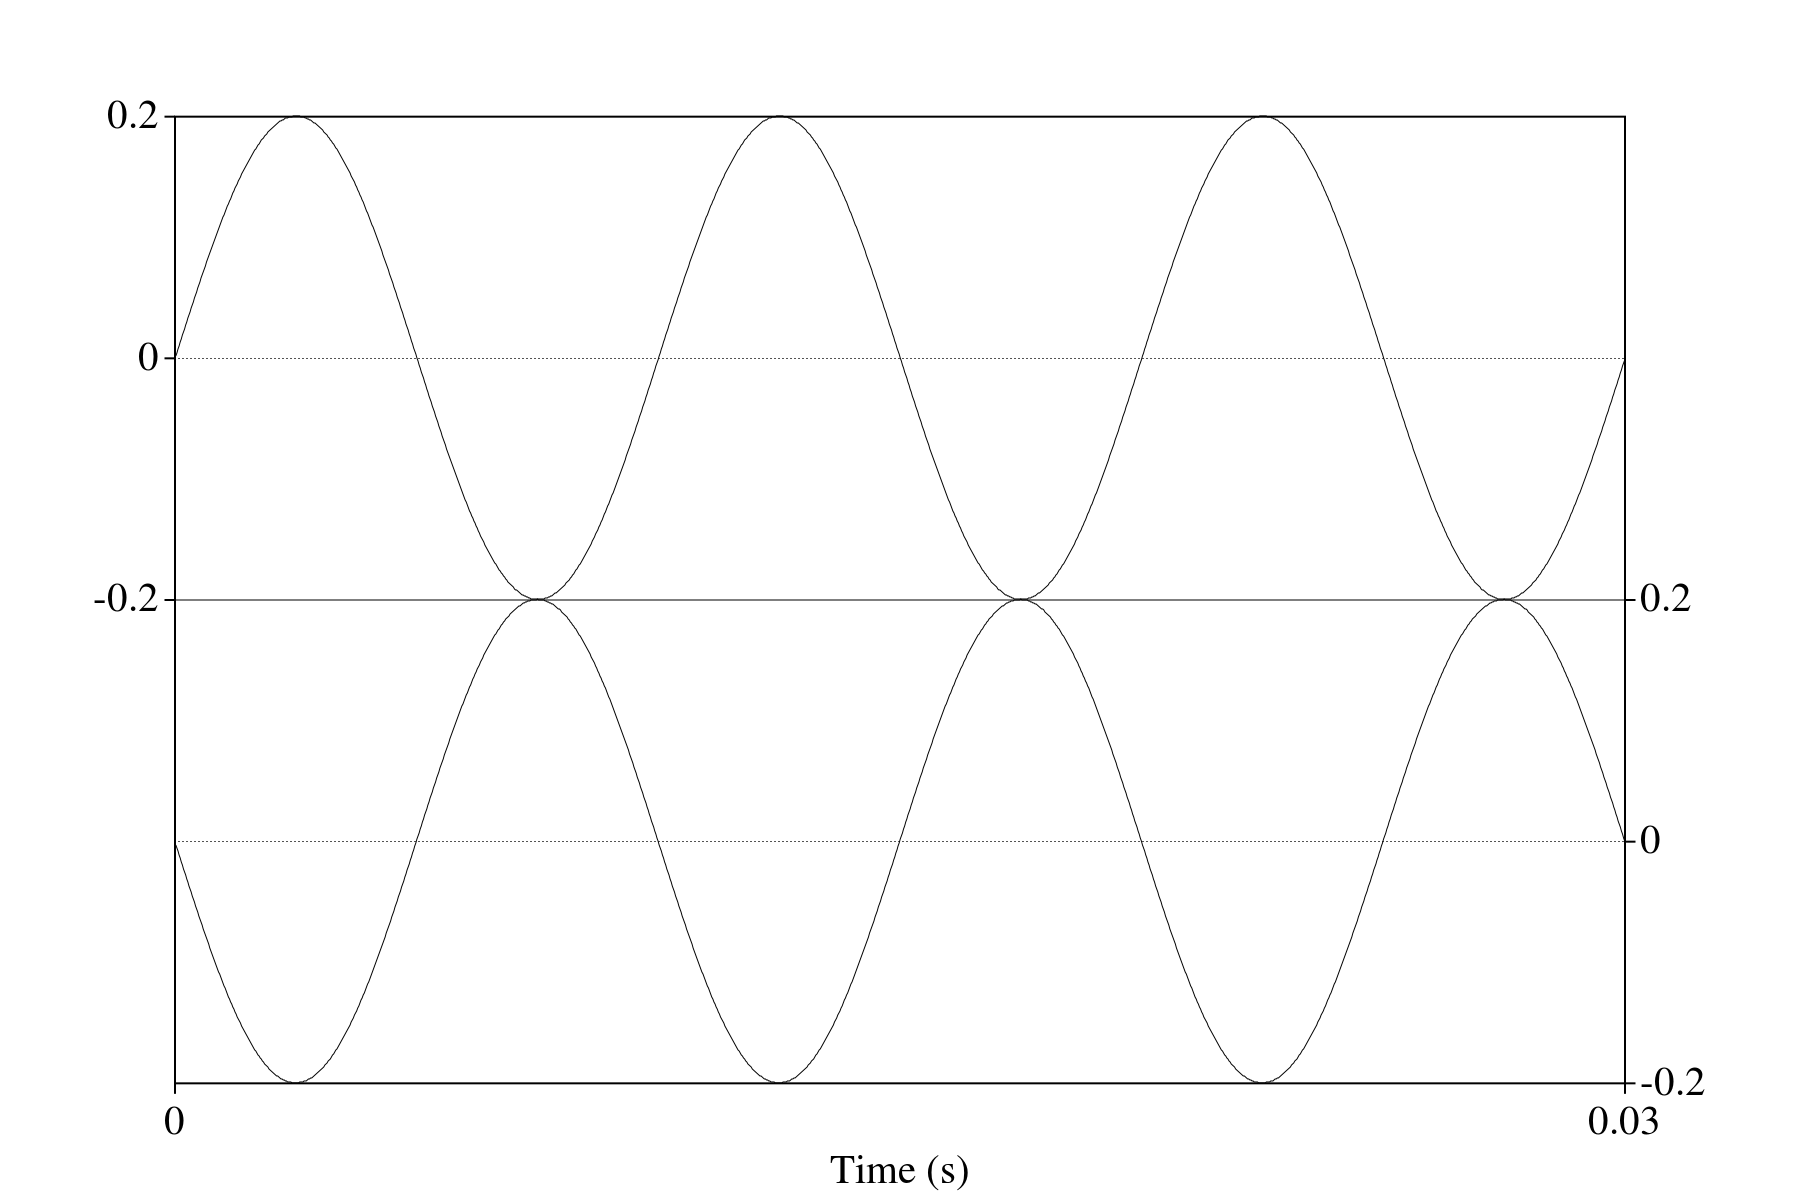
\includegraphics[width=\textwidth]{figure/wave-out-of-phase.png}
  \caption{Two sound waves with frequency of 100 Hz and the same amplitude, completely out of phase.}
  \label{fig:wave-out-of-phase2}
\end{subfigure}
\qquad
\begin{subfigure}{0.5\textwidth}
  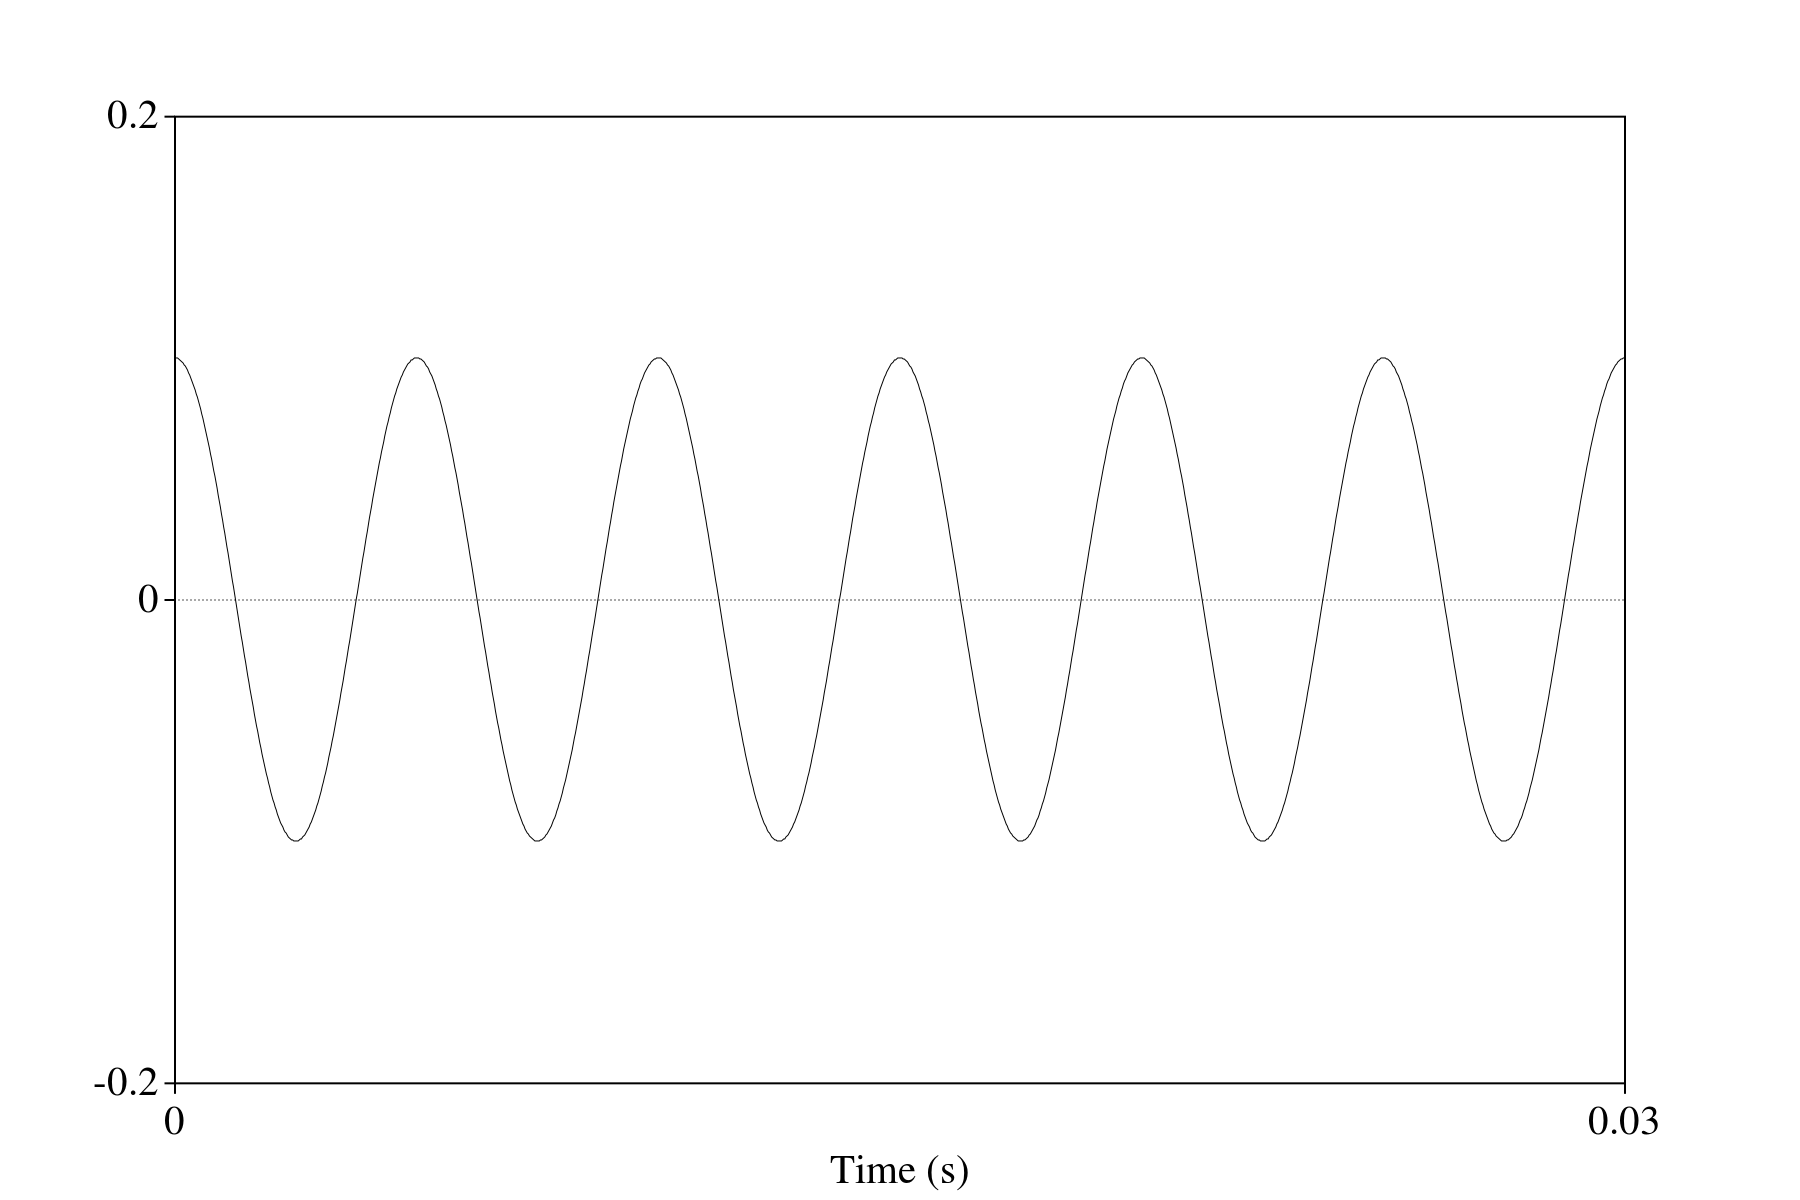
\includegraphics[width=\textwidth]{figure/sound-wave-addition-200hz-shifted.png}
  \caption{The sound wave resulting from the combination of the two out of phase waves in Fig. \ref{fig:wave-out-of-phase}.}
  \label{fig:wave-addition-200hz-shifted}
\end{subfigure}
%
\begin{center}
\begin{subfigure}{0.5\textwidth}
  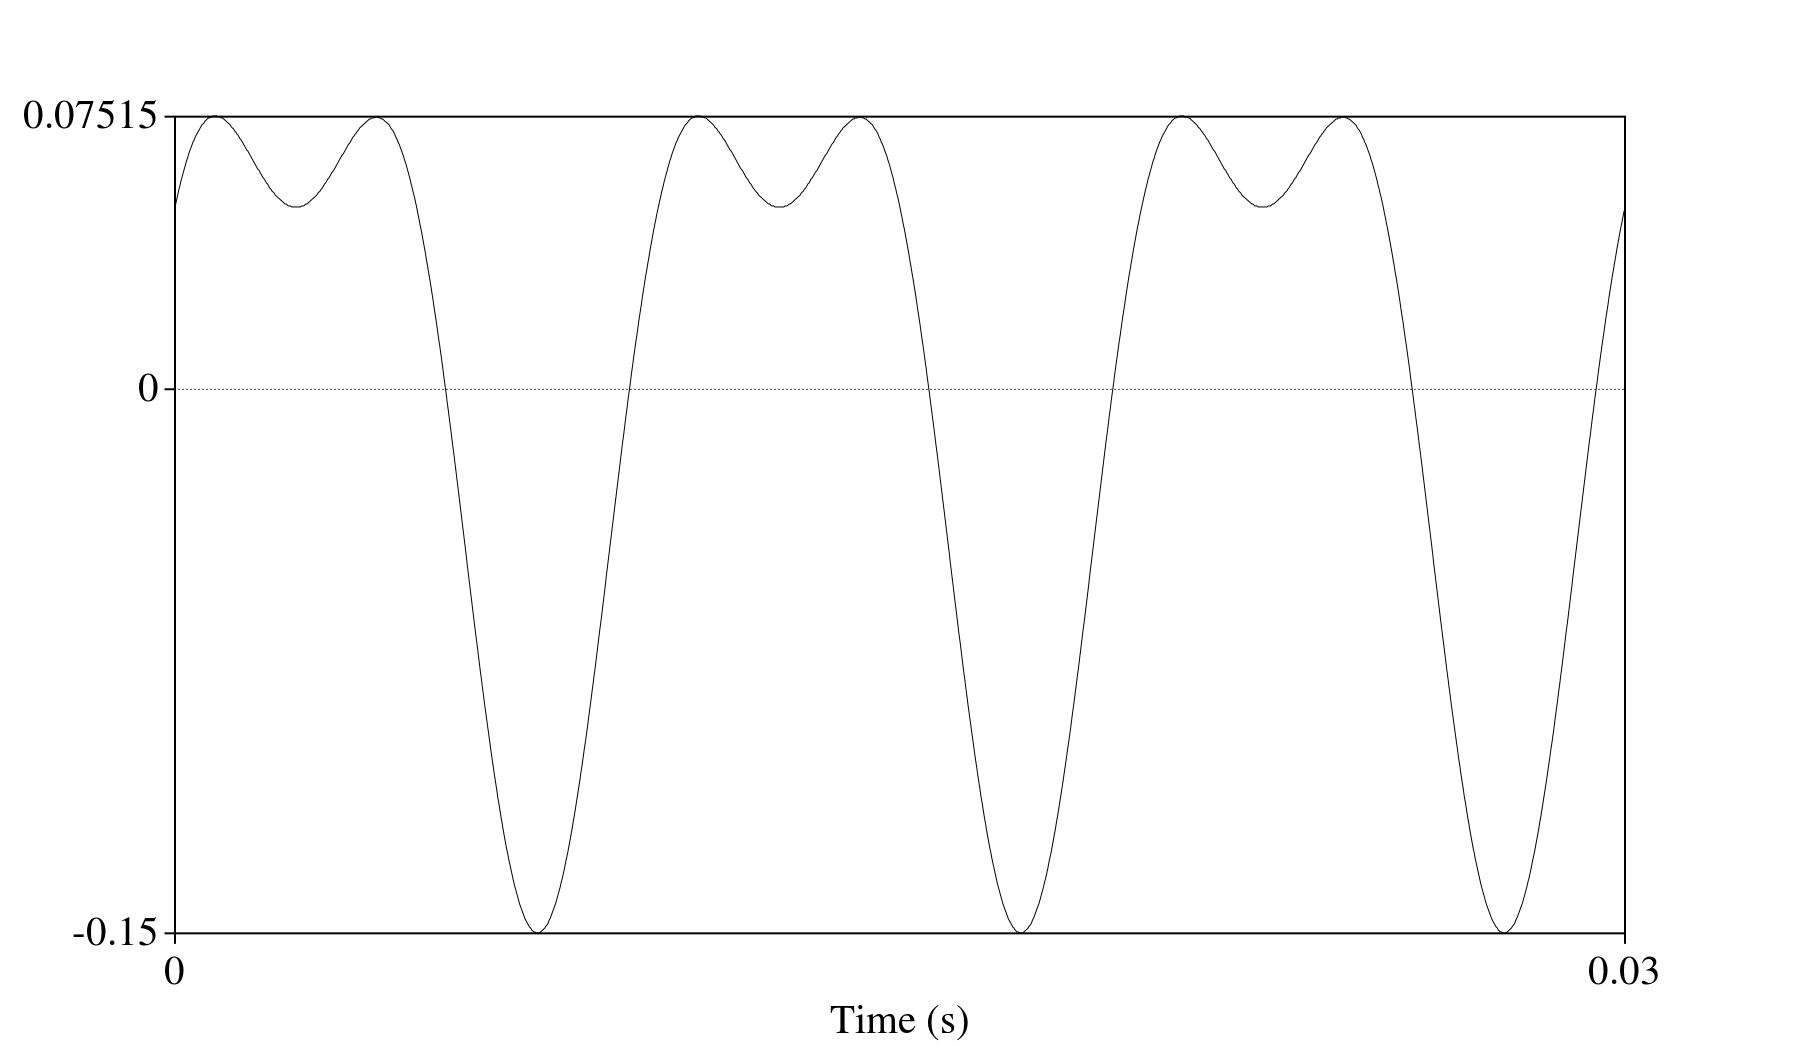
\includegraphics[width=\textwidth]{figure/sound-combined-shifted-phase.png}
  \caption{The sound wave resulting from the combination of the two out of phase waves in Fig. \ref{fig:wave-out-of-phase}.}
  \label{fig:sound-combined-shifted-phase}
\end{subfigure}
\end{center}
\caption{Demonstration of the combination of the same two waves as in Fig. \ref{fig:sound-wave-addition}, where the phase of the 200 Hz wave in Fig. \ref{fig:sound-wave-B} was shifted slightly (cf. Fig. \ref{fig:wave-addition-200hz-shifted})}
\label{fig:sound-shifted-phase}
\end{figure}

The combination of waves from multiple sound sources increases greatly in complexity as the number of sources increases, and the sounds originating from the sources are complex (ie. containing multiple frequency elements), such as speech.  Speech rarely occurs in isolation from from all external sound, yet we are still to largely understand speech in everyday environments; for example it is generally easy for humans to understand the speech of an interlocutor while sitting on a bench at a park.

The auditory system is actually quite skilled at identifying separate sources, even complex ones, like speech. Despite the shifted phase in Figure \ref{fig:sound-shifted-phase}, the human auditory system would still be able to detect and identify two separate waves.  While it undoubtedly plays a part, the differences in phase of combined signals does not normally completely negate a signal, nor render it unintelligible.  It is for this reason, and the complexity of phase calculations, that most efforts to remove speech from noise ignore the phase component.

\subsection{Difficulties of Speech in Noise}\DIFaddbegin \label{sec:snr-difficult}
\DIFaddend 

Nevertheless, there are still situations in which it is difficult to parse speech in noise.  This is most often due to signals with energy at similar frequencies that overlap.  The greater the amplitude of a signal at frequencies overlapping with those of speech, the more difficult the speech will be to understand.  This can be visualized in the spectrograms of the sentence ``A rich farm is rare in this sandy waste.'' in Figure \ref{fig:signal-SNR-intro}.  \DIFdelbegin \DIFdel{In }\DIFdelend \DIFaddbegin \DIFadd{As demonstrated before in }\DIFaddend Figure \ref{fig:signal-SNR-intro-high}, the amplitude, or loudness, of the noise is well below that of speech, which would likely be easily understand by a listener.  Figure \ref{fig:signal-SNR-intro-low} has a much greater noise amplitude level compared to the amplitude level of speech and consequently would likely be more difficult for a listener to understand.
\DIFdelbegin %DIFDELCMD < 

%DIFDELCMD < \begin{figure}[h!]
%DIFDELCMD < \centering
%DIFDELCMD < \begin{subfigure}{0.75\textwidth}
%DIFDELCMD <   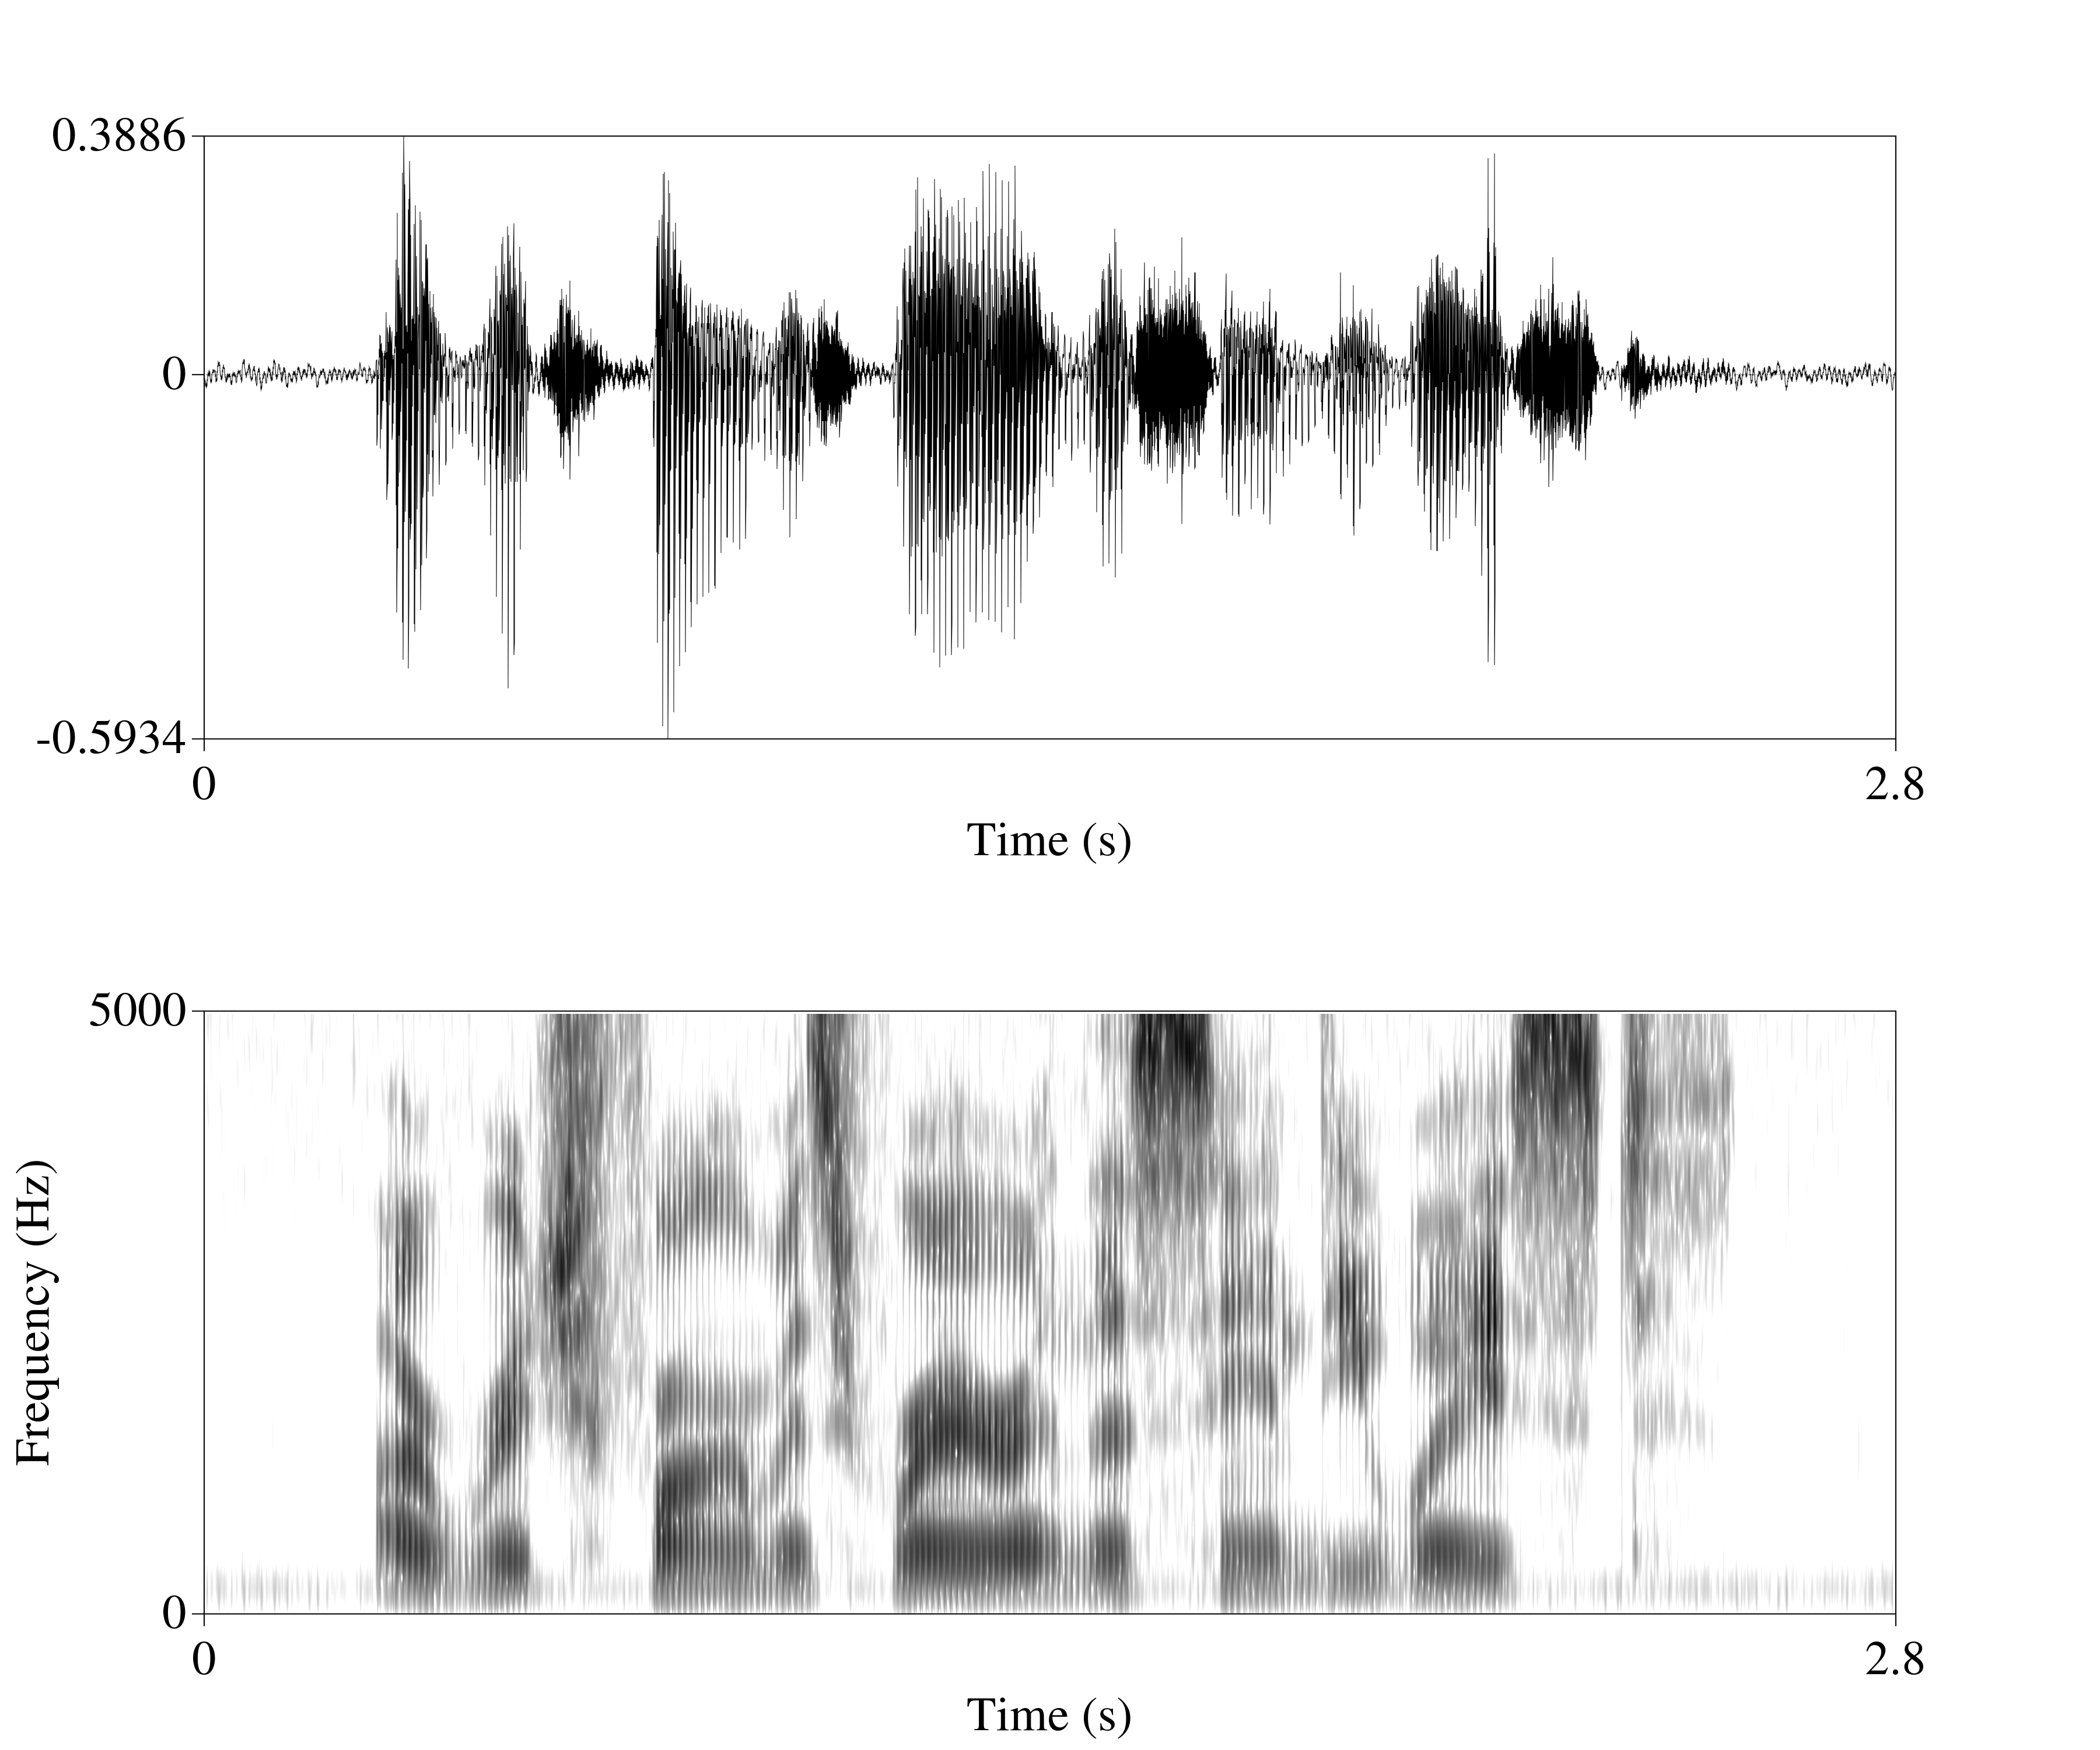
\includegraphics[width=.9\textwidth]{figure/signal-SNR-intro-high.png}
%DIFDELCMD <   %%%
%DIFDELCMD < \caption{%
{%DIFAUXCMD
\DIFdel{A sentence spoken with a low level of background noise, resulting in a }\textit{\DIFdel{high}} %DIFAUXCMD
\DIFdel{SNR.}}
  %DIFAUXCMD
%DIFDELCMD < \label{fig:signal-SNR-intro-high}
%DIFDELCMD < \end{subfigure}
%DIFDELCMD < %%%
%DIF < 
%DIFDELCMD < \begin{subfigure}{0.75\textwidth}
%DIFDELCMD <   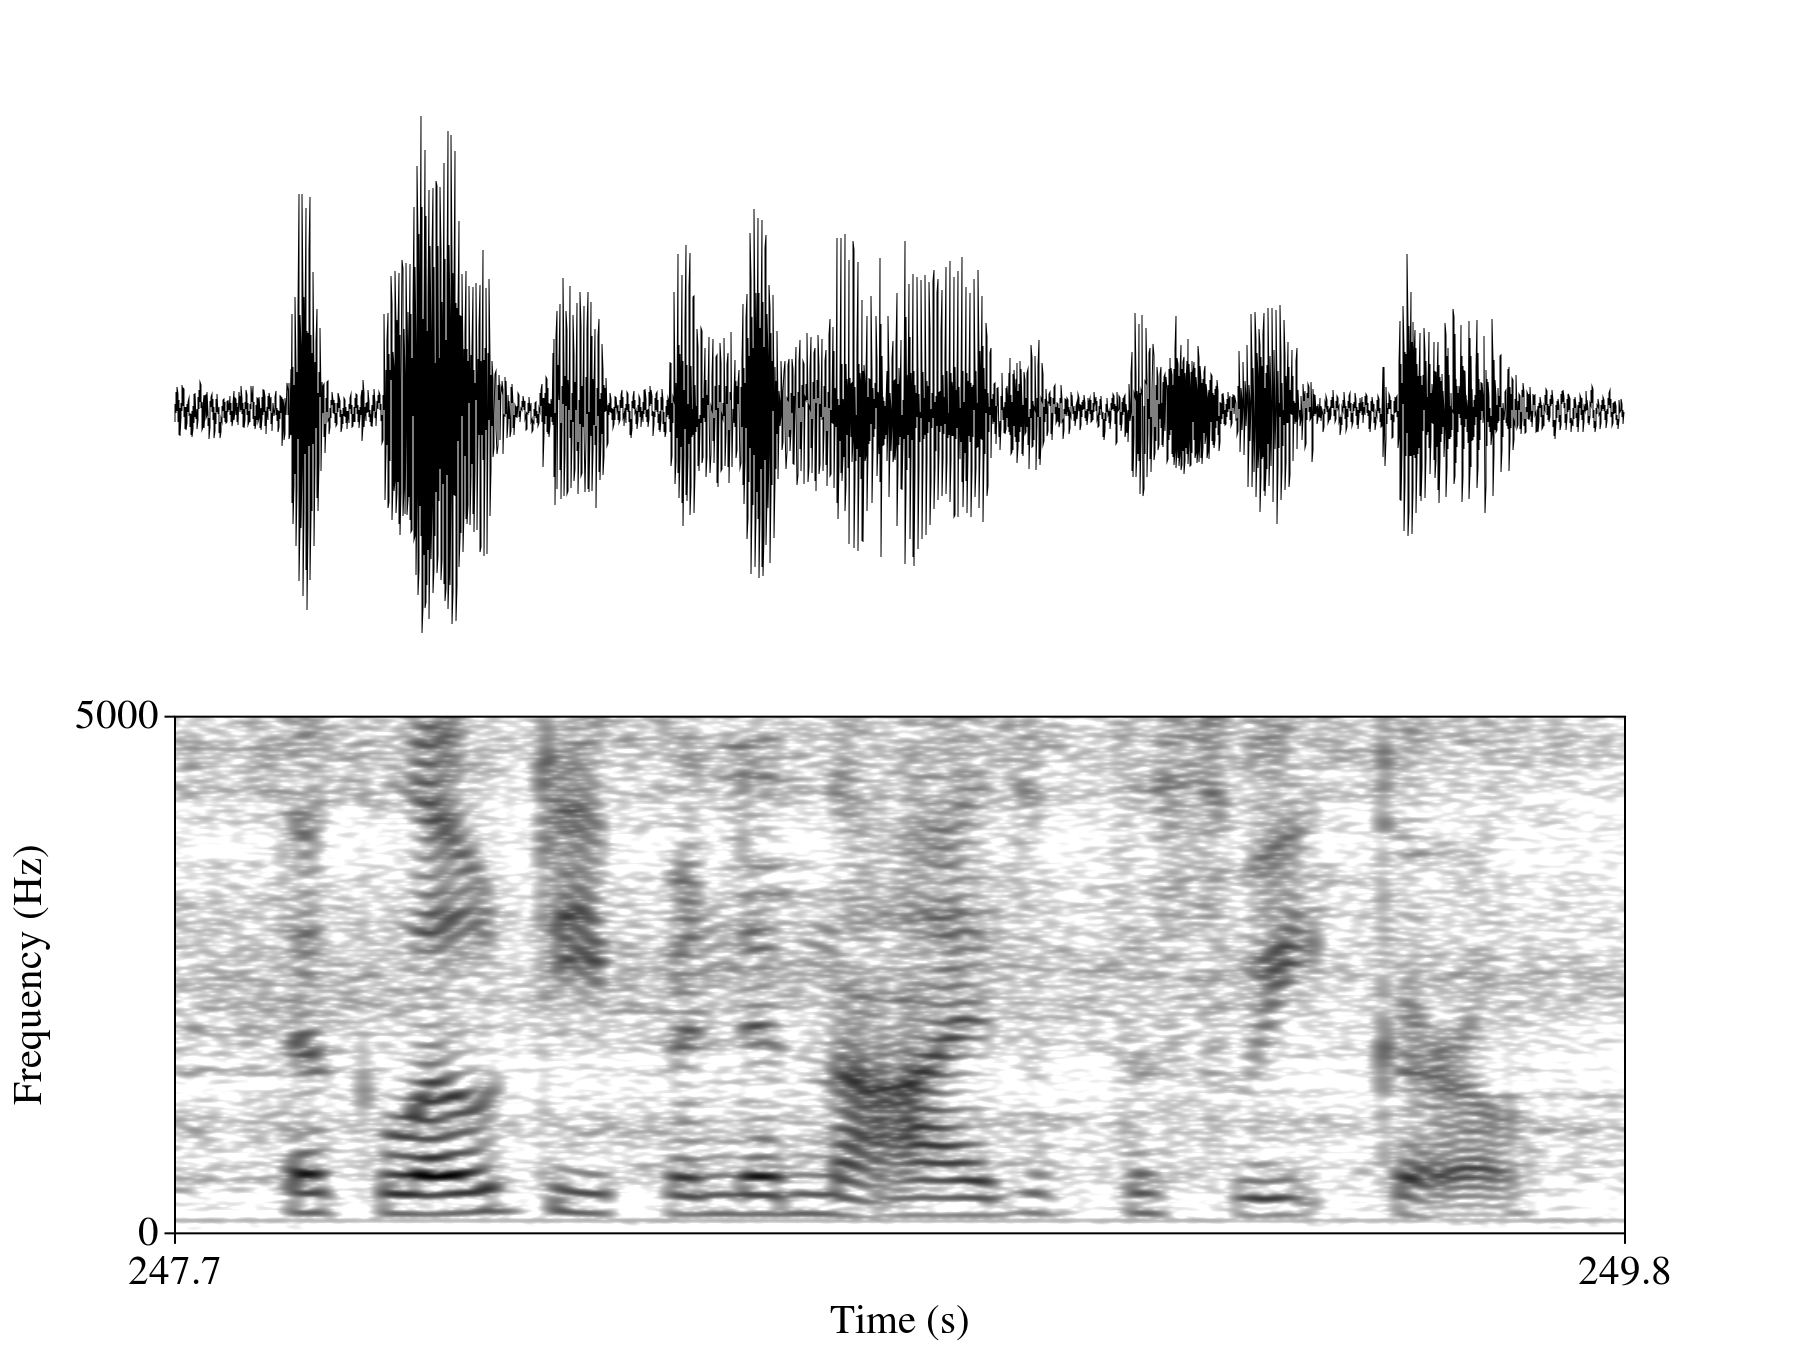
\includegraphics[width=.9\textwidth]{figure/signal-SNR-intro-low.png}
%DIFDELCMD <   %%%
%DIFDELCMD < \caption{%
{%DIFAUXCMD
\DIFdel{A sentence spoken with a high level of background noise, resulting in a }\textit{\DIFdel{low}} %DIFAUXCMD
\DIFdel{SNR.}}
  %DIFAUXCMD
%DIFDELCMD < \label{fig:signal-SNR-intro-low}
%DIFDELCMD < \end{subfigure}
%DIFDELCMD < %%%
%DIFDELCMD < \caption{%
{%DIFAUXCMD
\DIFdel{Waveforms and spectrograms of the sentence ``A rich farm is rare in this sandy waste''.}}
%DIFAUXCMD
%DIFDELCMD < \label{fig:signal-SNR-intro}
%DIFDELCMD < \end{figure}
%DIFDELCMD < %%%
\DIFdelend 

This relationship between speech and any background noise is called the signal to noise ration (SNR).  A complex signal with a higher signal to noise ratio (cf. Fig \ref{fig:signal-SNR-intro-high}) is generally easier to understand, because the amplitude of the speech (the `signal' of interest) is much greater than that of the noise.  Consequently a lower SNR (cf. Fig. \ref{fig:signal-SNR-intro-low}) results in speech that is more difficult to understand, because the amplitude of the speech is close to - or below - the amplitude of the background noise.

This poses a problem for human listeners, but generally is more difficult to deal with in automatic speech recognition (ASR), since the electronic device does not contain a highly-skilled, built-in auditory cortex.  There are a number of ways which have been proposed to deal with noise in a speech signal, both for human and automatic speech recognition.  These will be discussed further in Chapters \ref{chapter3} and \ref{chapter4}.

\section{Overview of Dissertation}\label{ch1:diss-overview}

This report aims to explore a novel method of human speech perception and automatic speech recognition (ASR) in noisy environments.  The method proposes that speech be recorded from the inside of the ear canal of the speaker, slightly transformed, and sent to the human listener or the computer receiver for recognition.  Collecting speech from the ear allows for usage of the human skull and adjacent tissues to passively filter out the noisy environment, leaving only - or mostly - the human speech carrying the intended message.  

The intention of this study is to determine a) if recording human speech from the inside of the ear canal can significantly reduce background noise in a signal, b) if intelligible speech, suitable for communication, can be collected from the inside of the ear canal, c) if humans find speech recorded from the ear canal more intelligible than speech in noisy conditions, and finally d) if ASR systems are able to recognize speech recorded in the ear canal with greater accuracy than speech recorded in noise.

Since currently there is no established corpus of data that contain speech recorded from the inside of the ear canal together with speech simultaneously recorded from the mouth in noisy environments, it was necessary to record speakers in this environment and create a new corpus.  The theory behind the acoustics of recording speech from the ear canal, as well as the process for developing this corpus are described in Chapter \ref{chapter2}, along with a discussion of the recorded speech.  Chapter \ref{chapter3} will outline a human perception experiment, tasking listeners with the transcription of various sentences of speech recorded at the mouth in noise in noise, and recorded from the ear.   Chapter \ref{chapter4} describes the use of this same speech with an ASR system, and its recognition performance.  Chapter \ref{chapter5} will summarize the previous chapters and engage in an overall discussion of the implications of the results, the limitations of the present experiments and methods, and suggestions for future research direction.



% %set_parent(‘/Users/mwilli/Documents/Spring_2017/Dissertation_Document/Dissertation_Working_Directory_Draft/Dissertation_Main.Rnw')
% 
% <<chunk_options, echo=FALSE>>=
% # This is where we set basic knitr options.
% opts_chunk$set(echo=TRUE, message=FALSE, warning = TRUE, cache = FALSE, comment="")
% options(width=75) # This sets how wide the R printout can be.
% @
% 
%  <<setup-child, include=FALSE>>=
%  set_parent('/home/sam/Dissertation/Dissertation_Template/Dissertation_Main_Template/Dissertation_Main.Rnw')
% @
% 
% <<load_libraries, echo=FALSE>>=
% library(tidyr)
% library(dplyr)
% library(ggplot2)
% library(lme4)
% library(lsmeans)
% library(car)
% library(pbkrtest)
% library(xtable)
% library(cowplot)
% library(plyr)
% @



\chapter{Ear-Recorded Speech\label{chapter2}}


\section{Introduction}

The accuracy of automatic speech recognition (ASR) has significantly improved over the past several years; similar, but less dramatic improvements have been made regarding the challenging task of recognizing speech in noisy environments (\cite{zhang:17}).  The performance of the latter still falls below the accuracy that most human listeners achieve.  Even human listeners and the \DIFaddbegin \DIFadd{human }\DIFaddend auditory system has limits \DIFaddbegin \DIFadd{and }\DIFaddend is only able to remove a \DIFdelbegin \DIFdel{limited }\DIFdelend \DIFaddbegin \DIFadd{certain }\DIFaddend amount of noise from a speech signal before that signal becomes completely unintelligible.  The primary issue arises from the fact that speech normally passes from a speaker's mouth into either the ear (human speech perception) or a microphone (ASR), but the passage of speech through the medium of air allows corruption of the signal by noise of unknown loudness and unpredictable source.  

This research proposed eliminating, by and large, the passage of speech through air by recording the speech in an unconventional location - from the inside of the \textit{speaker's} ear canal.  Speech is not only emitted from the oral cavity, but the vibrations also pass throughout the human body.  Using the ear canal as the source of speech adds the benefit that the entrance to the ear canal can be securely occluded behind the microphone (eg. with a noise reduction device such as an ear-plug).  Ambient noise from the air is largely filtered out by both the occlusion device and the human skull.

Due to the very specific nature of the requirements for this study (that the speech data recorded needed to be recorded from the ear), it was necessary to record data from scratch, as the author was not aware of another corpus of ear-recorded speech that existed at the time of this study.  This corpus \DIFdelbegin \DIFdel{contains }\DIFdelend \DIFaddbegin \DIFadd{aimed to collect }\DIFaddend speech recorded from \DIFdelbegin \DIFdel{two microphones simultaneously: one }\DIFdelend \DIFaddbegin \DIFadd{a microphone }\DIFaddend placed at the mouth \DIFdelbegin \DIFdel{, and the other }\DIFdelend \DIFaddbegin \DIFadd{(in noisy and clean environments), and another microphone placed }\DIFaddend at the ear \DIFdelbegin \DIFdel{. The goal for this new corpus is to offer a comparison between these two recording locations. The recognition ability of humans and ASR systems on the ear-recorded speech could also be tested.  Both clean and noisy speech were desired}\DIFdelend \DIFaddbegin \DIFadd{(in the same environments)}\DIFaddend . Owing to the variability that occurs when even the same speaker repeats the same sentence, speech critically needed to be recorded from the two locations simultaneously.  \DIFdelbegin \DIFdel{This }\DIFdelend \DIFaddbegin \DIFadd{The goal for this new corpus is to offer a comparison between these two recording locations, and simultaneously recorded speech }\DIFaddend allows for a more accurate comparison\DIFdelbegin \DIFdel{of the two signals}\DIFdelend \DIFaddbegin \DIFadd{.  The goal for this corpus was to be used for testing humans' and ASR ability to understand speech in noise compared with their ability to understand speech recorded from the ear canal}\DIFaddend .


The initial experiment described in Section \ref{expt1} below was a data collection experiment.  It aimed to create \DIFdelbegin \DIFdel{a small }\DIFdelend \DIFaddbegin \DIFadd{this }\DIFaddend corpus of speech recorded from the ear canal \DIFaddbegin \DIFadd{and from the mouth }\DIFaddend for use in the following two experiments (cf. Chapters \ref{chapter3} and \ref{chapter4}).  The next section explains the theory behind the assumption that usable speech can be collected from the inside of one's ear canal.

\section{Background}



%DIF >  \subsection{Mouth-emitted Speech}
%DIF >  
%DIF >  \begin{wrapfigure}{l}{0.5\textwidth}
%DIF >  \centering
%DIF >    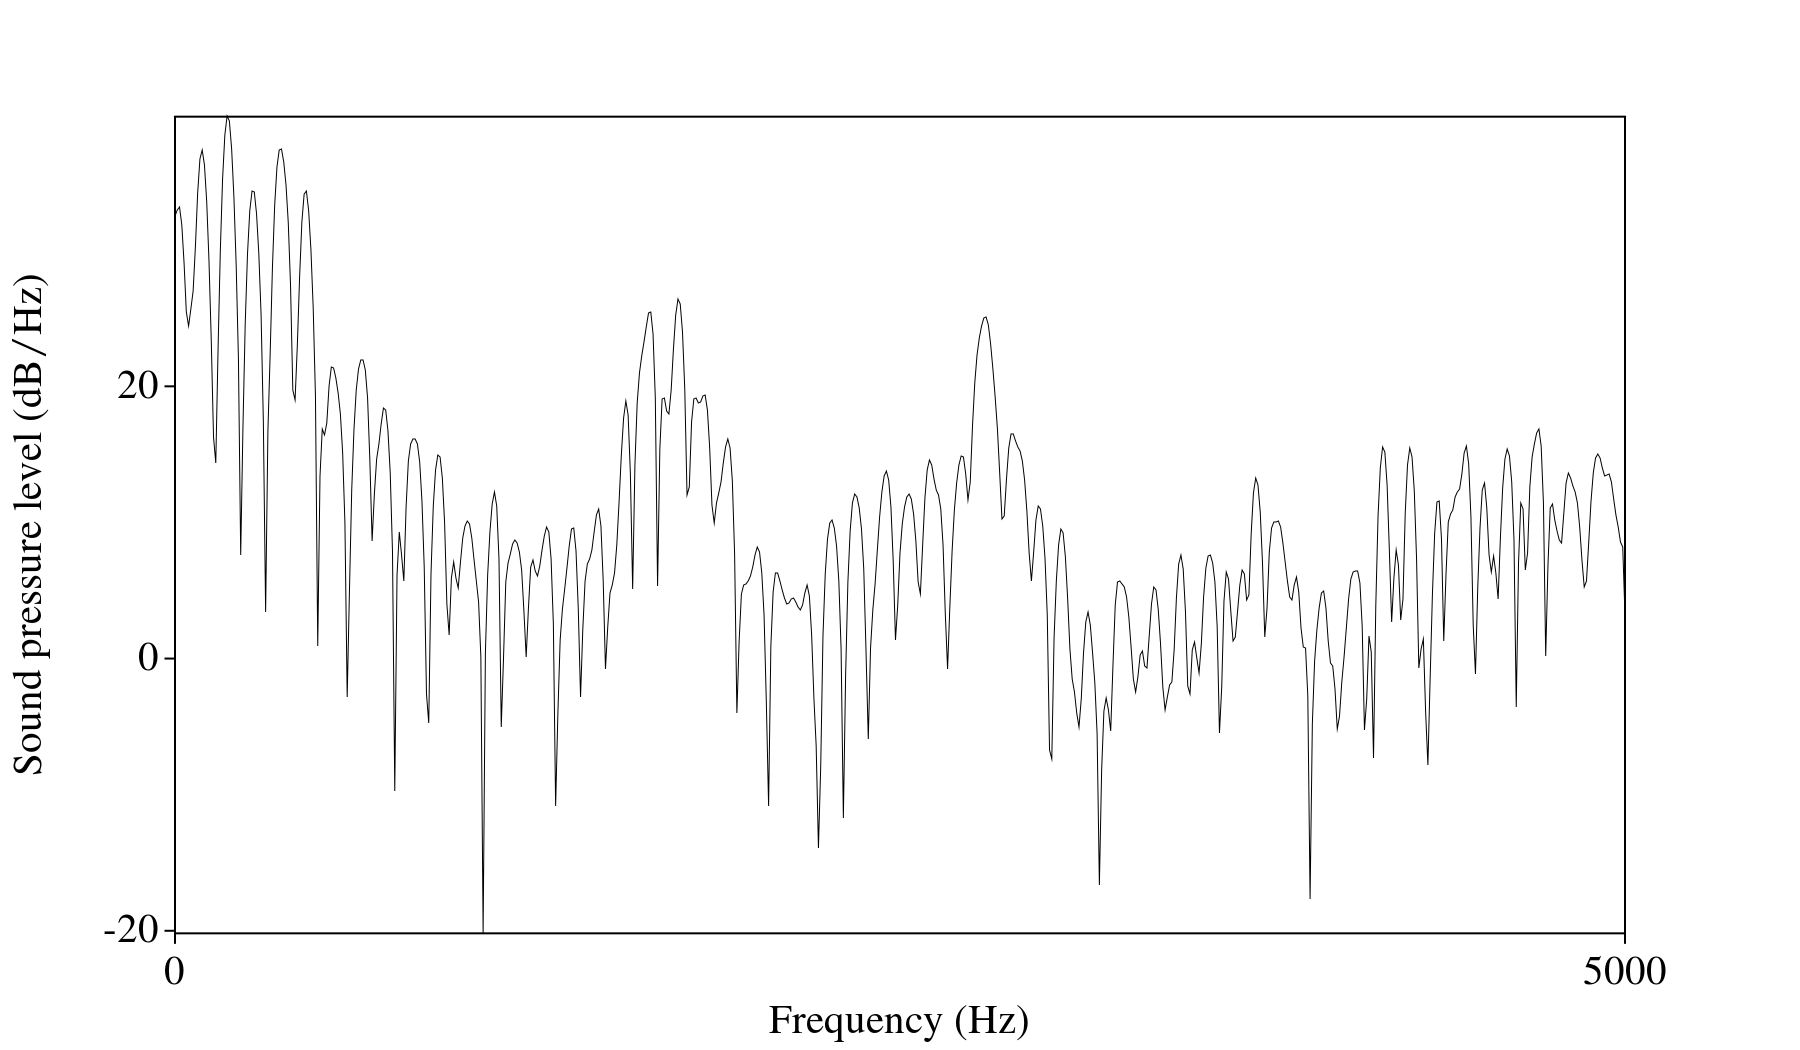
\includegraphics[width=0.5\textwidth]{figure/spctrm5k.png}
%DIF >    \caption{Spectrum of the middle of an /I/ vowel.  Each ``spike'' is a separate ``band'' of frequency, called a harmonic.}
%DIF >    \label{fig:spctrm5k}
%DIF >  \end{wrapfigure}
%DIF >  %
%DIF >  First, it is appropriate to review the acoustic structure of mouth-emitted speech.  Speech could be divided into two primary categories - voiced and unvoiced.  Voiced speech is composed of bands of acoustic energy, called harmonics, located along a frequency spectrum (cf. fig \ref{fig:spctrm5k}).  
%DIF >  %
%DIF >  Certain harmonics will be dampened by the vocal tract, leaving others relatively unfiltered.  A region of harmonics containing more energy are called formants.  The location, shape, and transition over time of these formants (among other more minor features) are what encodes speech information for voiced sounds.  A spectrogram is a graph used to conveniently diagram the amplitude of various frequencies over time (cf. fig \ref{fig:spctgrm1k5k}).
%DIF >  %
%DIF >  \begin{figure}[h!]
%DIF >  \begin{subfigure}{0.95\textwidth}
%DIF >    \centering
%DIF >    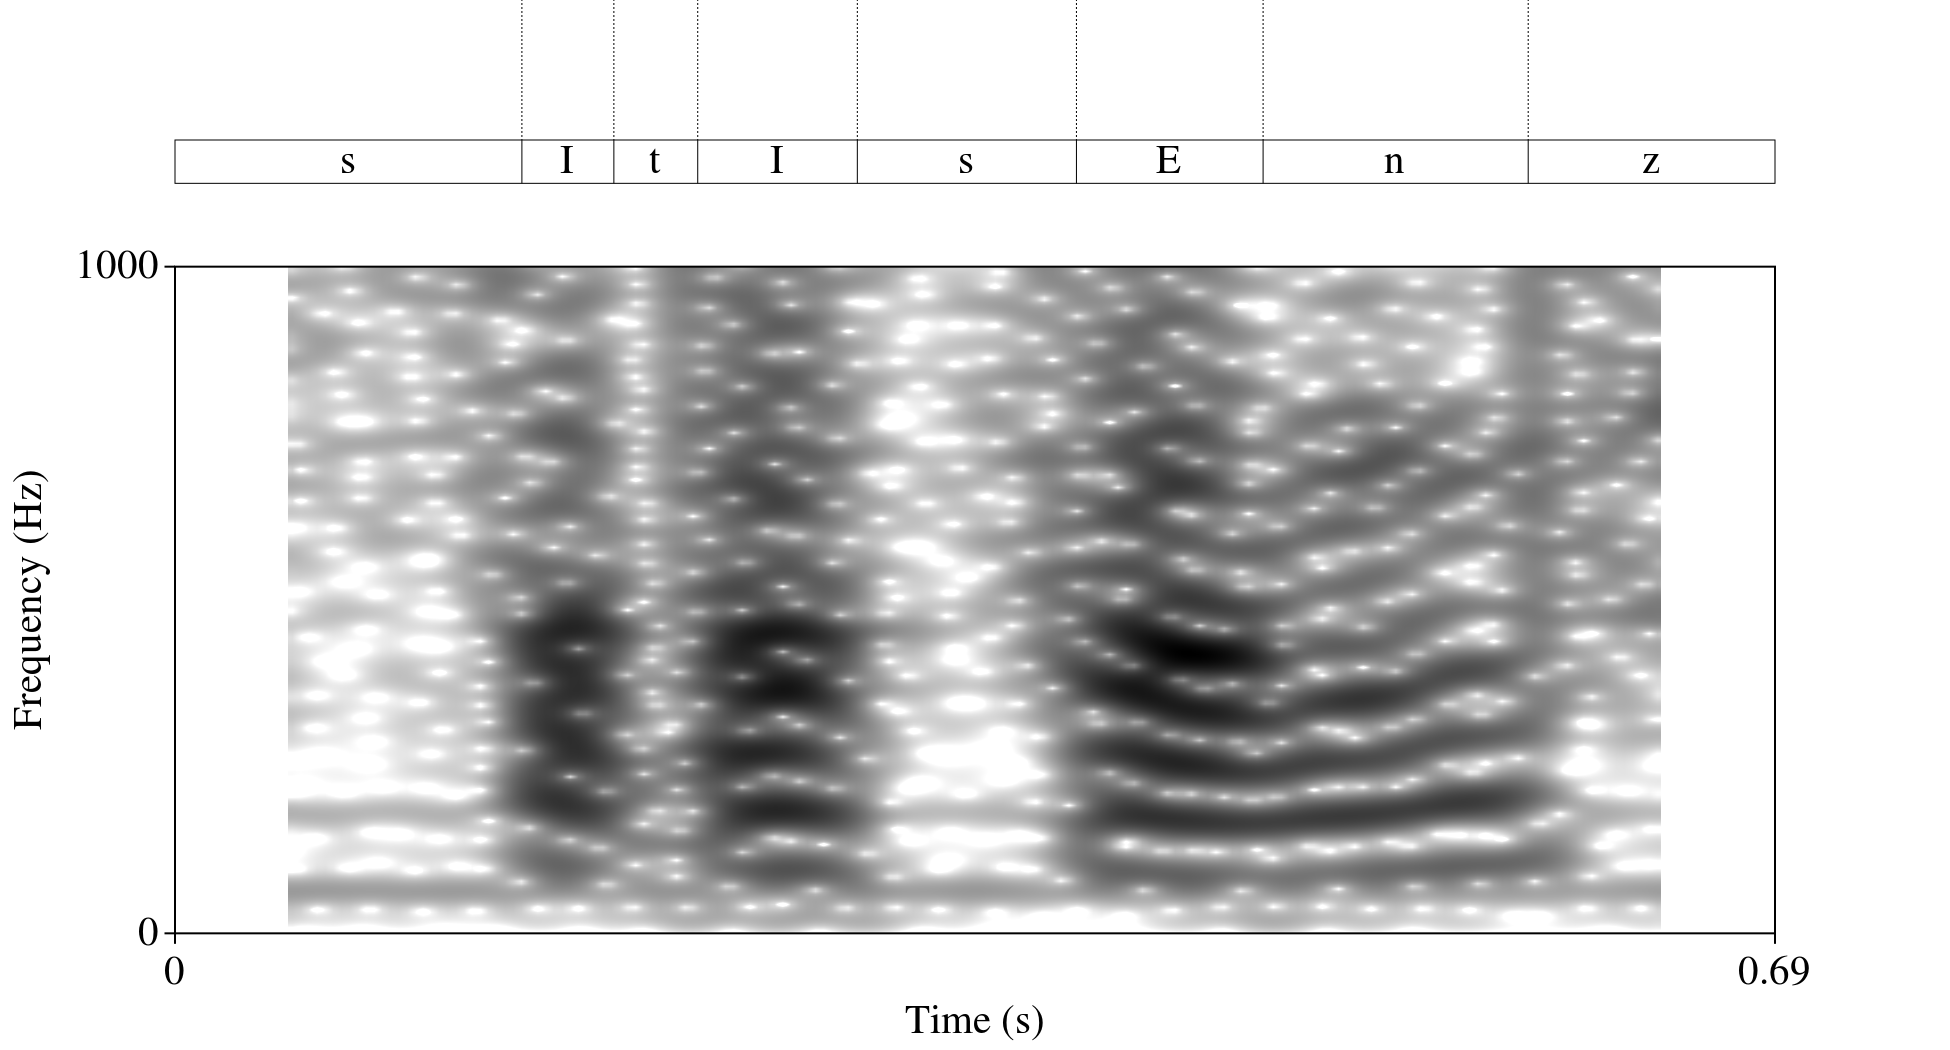
\includegraphics[width=0.95\textwidth]{figure/spctgrm1k.png}
%DIF >    \caption{Zoomed to the 0-1kHz range for better visualization of harmonics.}
%DIF >    \label{fig:spctgrm1k}
%DIF >  \end{subfigure}%
%DIF >  \hfill
%DIF >  \begin{subfigure}{0.95\textwidth}
%DIF >    \centering
%DIF >    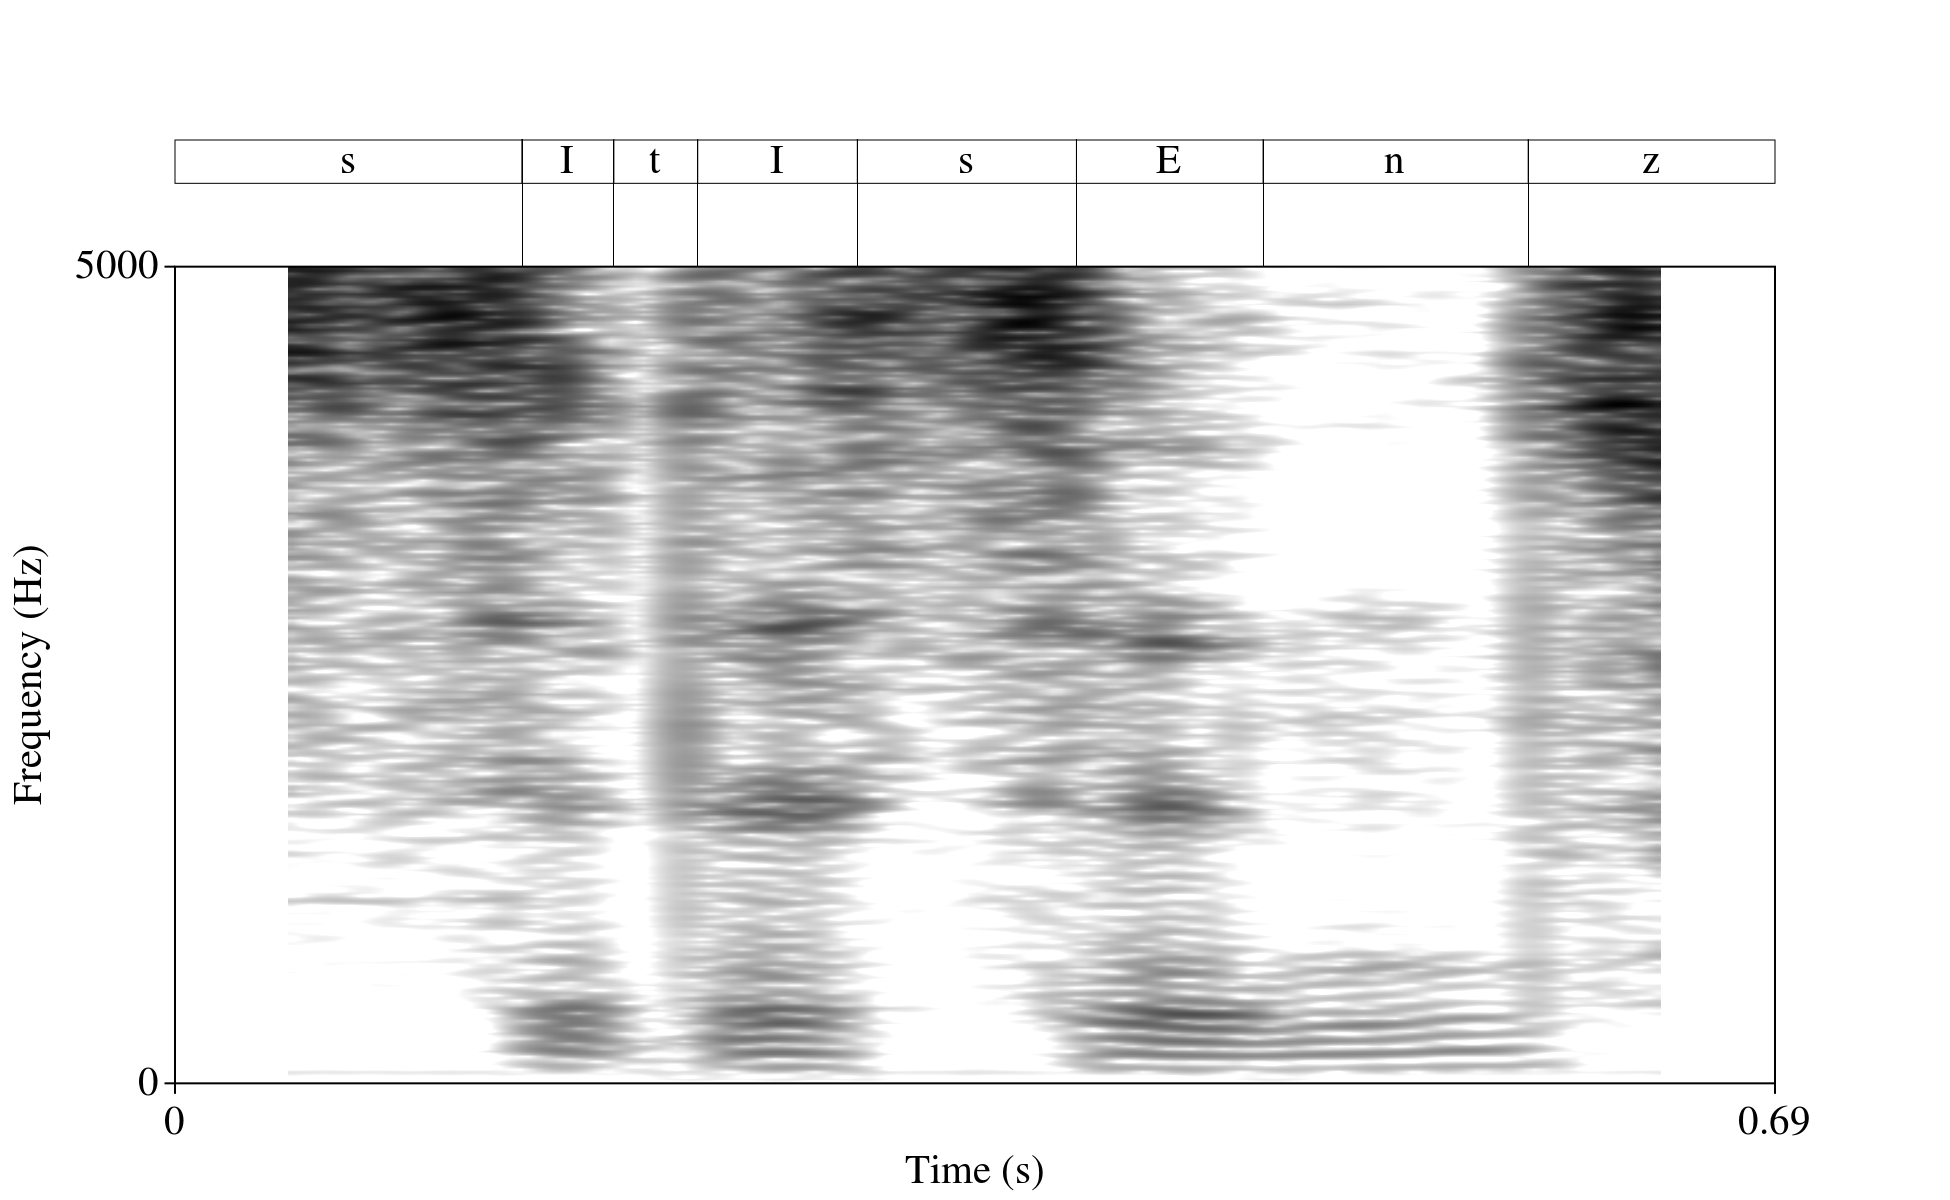
\includegraphics[width=0.95\textwidth]{figure/spctgrm5k.png}
%DIF >    \caption{Zoomed to a more standard 0-5kHz range.}
%DIF >    \label{fig:spctgrm5k}
%DIF >  \end{subfigure}
%DIF >  \caption{Spectrogram of the word ``citizen'' with phonetic transcription above.}
%DIF >  \label{fig:spctgrm1k5k}
%DIF >  \end{figure}
%DIF >  
%DIF >  For unvoiced speech, the information used to recognize and categorize the speech sound is likely found in either the turbulent frication generally centered in higher frequencies cf. fig \ref{fig:spctgrm_s} (although some of the information can be found in lower frequencies), or found in the voiced information in the transitions into and out of the sound (\cite{story:10}).
%DIF >  %
%DIF >  \begin{wrapfigure}{l}{0.5\textwidth}
%DIF >  \centering
%DIF >    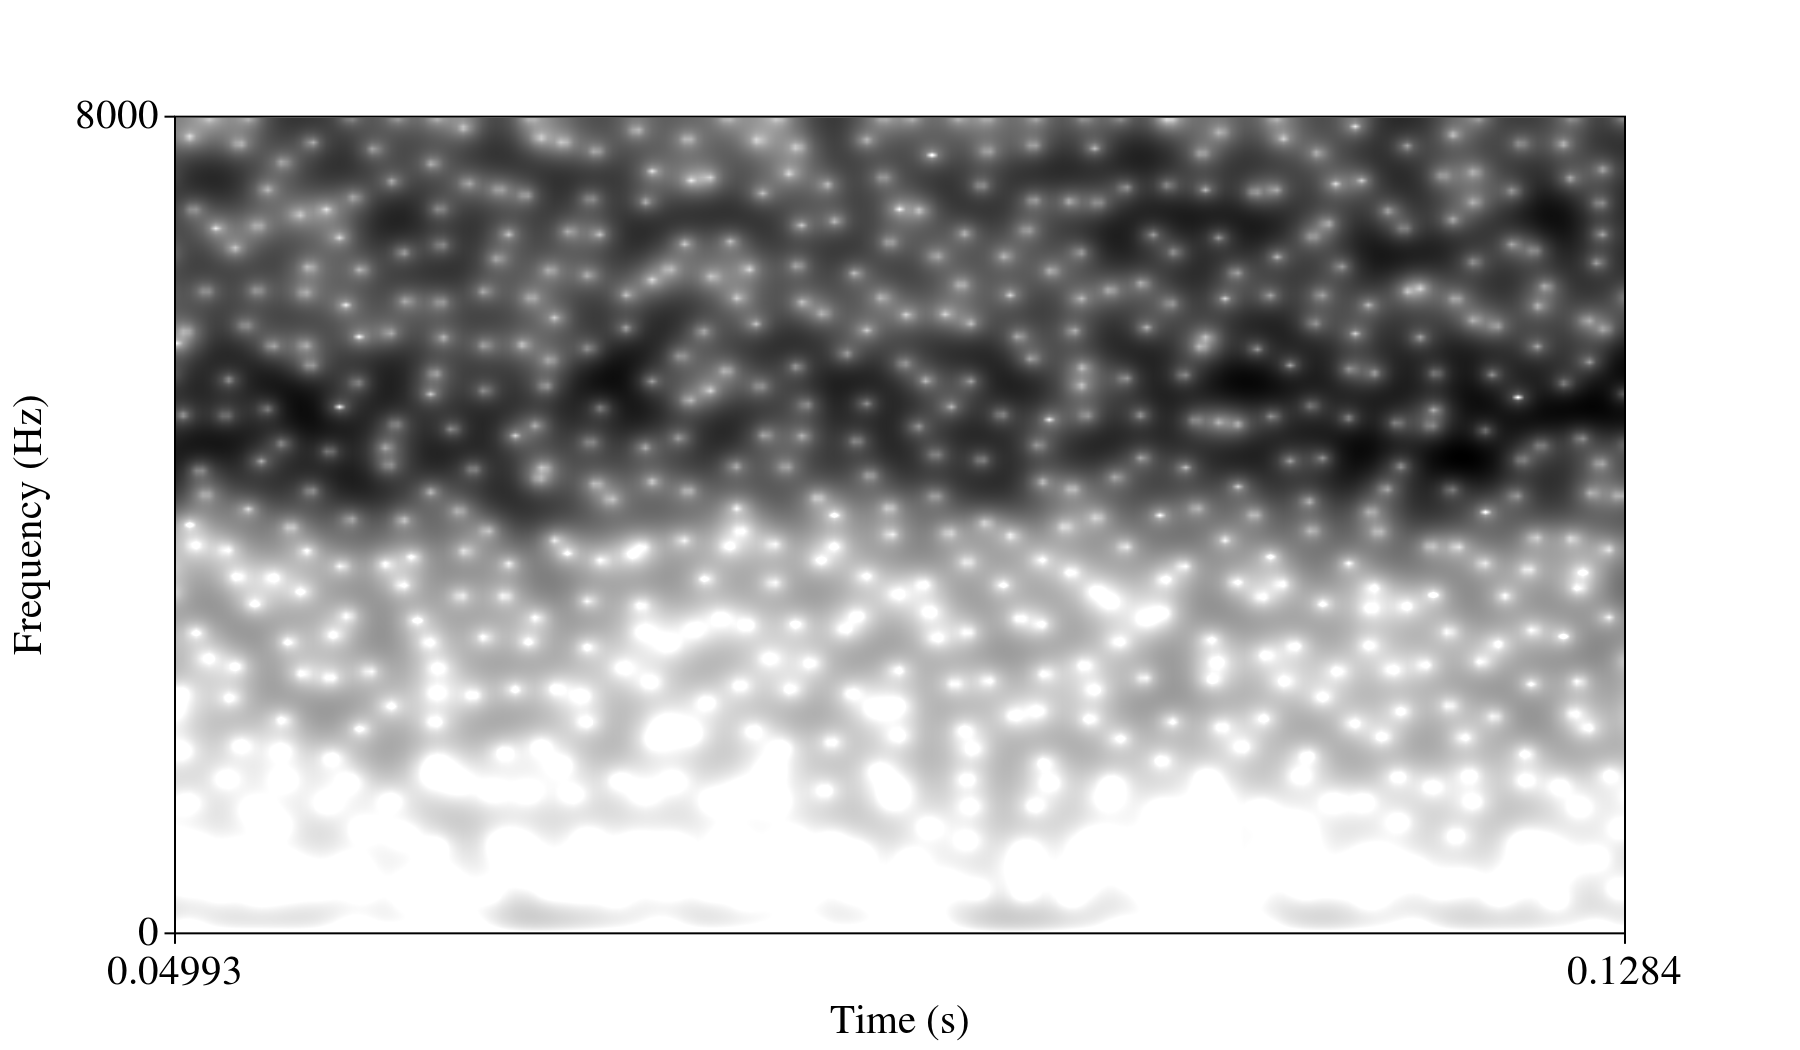
\includegraphics[width=0.5\textwidth]{figure/spctgrm_s.png}
%DIF >    \caption{Spectrum of the initial /s/ in ``citizen''. Zoomed to range of 0-8kHz for visualization of high frequency energy.}
%DIF >    \label{fig:spctgrm_s}
%DIF >  \end{wrapfigure}
\DIFaddbegin 

%DIF >  Discussion about Body/Bone conduction (mechanical)
%DIF >  \subsection{Bone Conduction}

\DIFaddend The speech vibrations of a person's own voice will propagate throughout the head and body\DIFdelbegin \DIFdel{(cf. Fig. \ref{fig:bekesyBodyTransfer}).}\DIFdelend \DIFaddbegin \DIFadd{.%DIF >  (cf. Fig. \ref{fig:bekesyBodyTransfer}).  
}\DIFaddend Of interest for the present study, these waves will pass through the tissue in the head, and enter into the ear canal, where they will be recorded. %DIF >  This brief section will discuss some of the known properties 

%DIF <  \subsection{Mouth-emitted Speech}
%DIF <  
%DIF <  \begin{wrapfigure}{l}{0.5\textwidth}
%DIF <  \centering
%DIF <    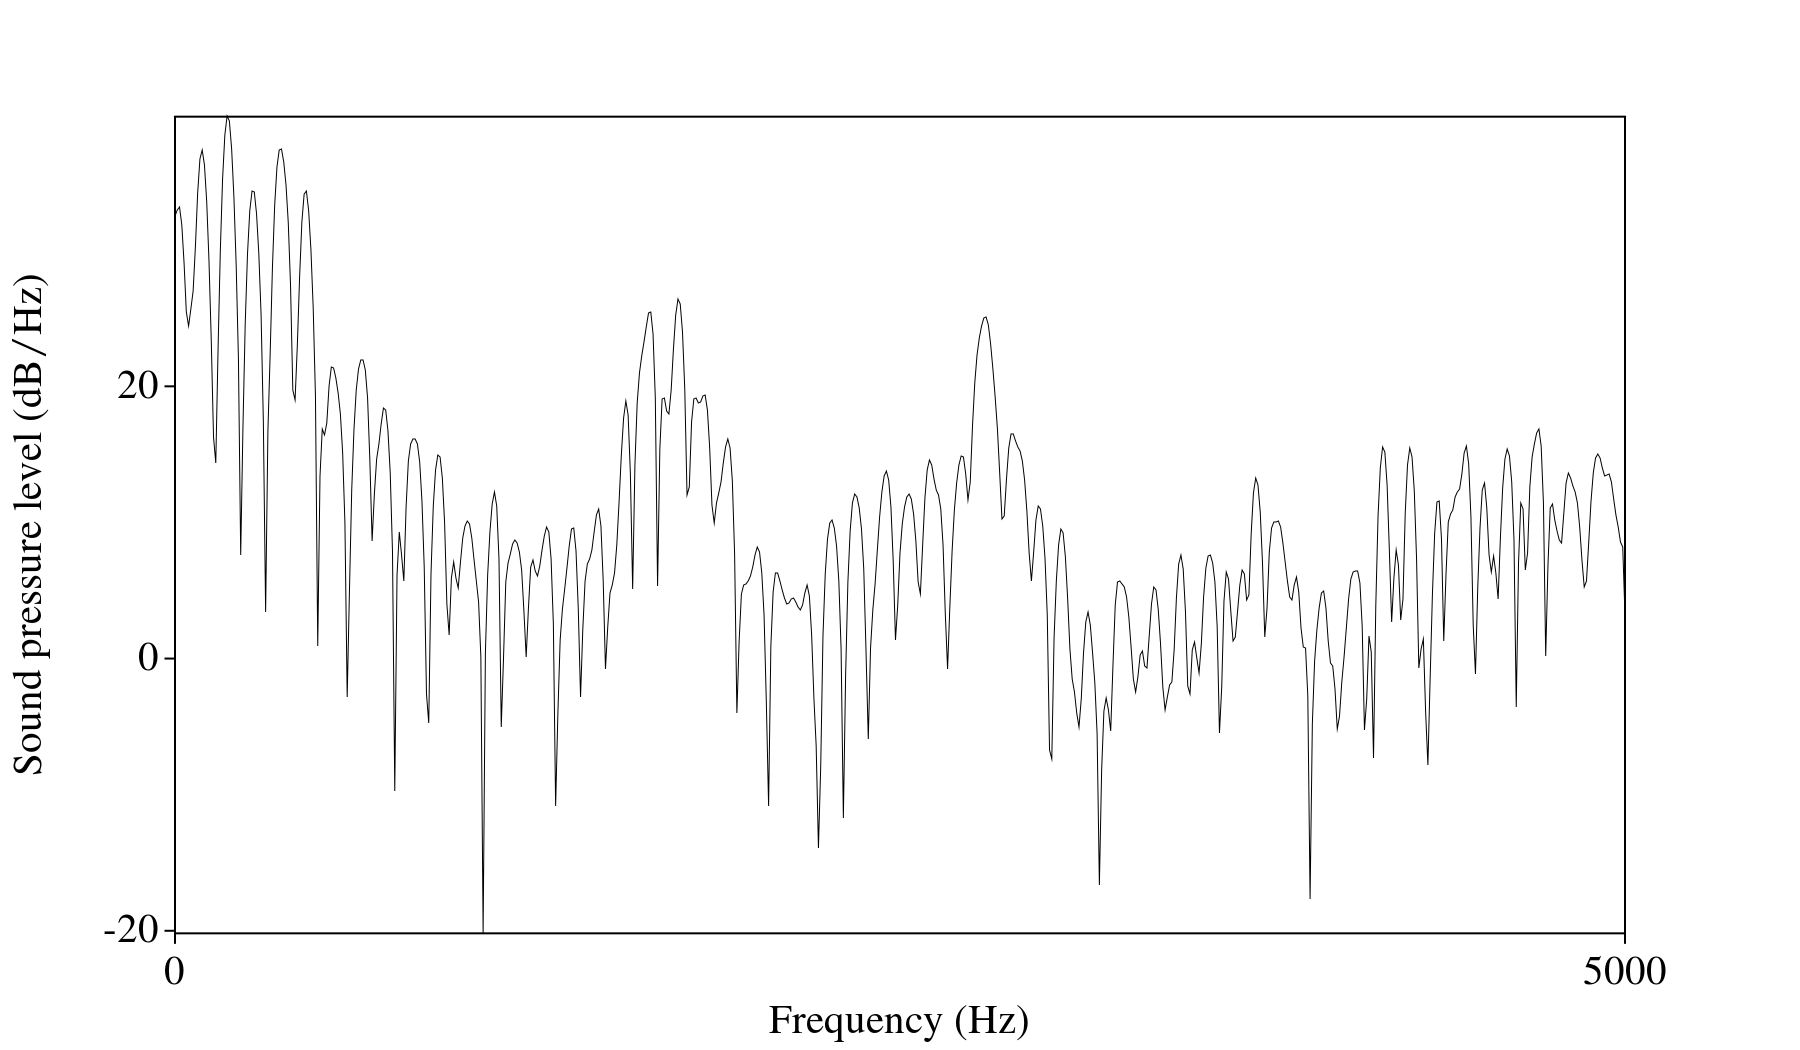
\includegraphics[width=0.5\textwidth]{figure/spctrm5k.png}
%DIF <    \caption{Spectrum of the middle of an /I/ vowel.  Each ``spike'' is a separate ``band'' of frequency, called a harmonic.}
%DIF <    \label{fig:spctrm5k}
%DIF <  \end{wrapfigure}
%DIF <  %
%DIF <  First, it is appropriate to review the acoustic structure of mouth-emitted speech.  Speech could be divided into two primary categories - voiced and unvoiced.  Voiced speech is composed of bands of acoustic energy, called harmonics, located along a frequency spectrum (cf. fig \ref{fig:spctrm5k}).  
%DIF <  %
%DIF <  Certain harmonics will be dampened by the vocal tract, leaving others relatively unfiltered.  A region of harmonics containing more energy are called formants.  The location, shape, and transition over time of these formants (among other more minor features) are what encodes speech information for voiced sounds.  A spectrogram is a graph used to conveniently diagram the amplitude of various frequencies over time (cf. fig \ref{fig:spctgrm1k5k}).
%DIF <  %
%DIF <  \begin{figure}[h!]
%DIF <  \begin{subfigure}{0.95\textwidth}
%DIF <    \centering
%DIF <    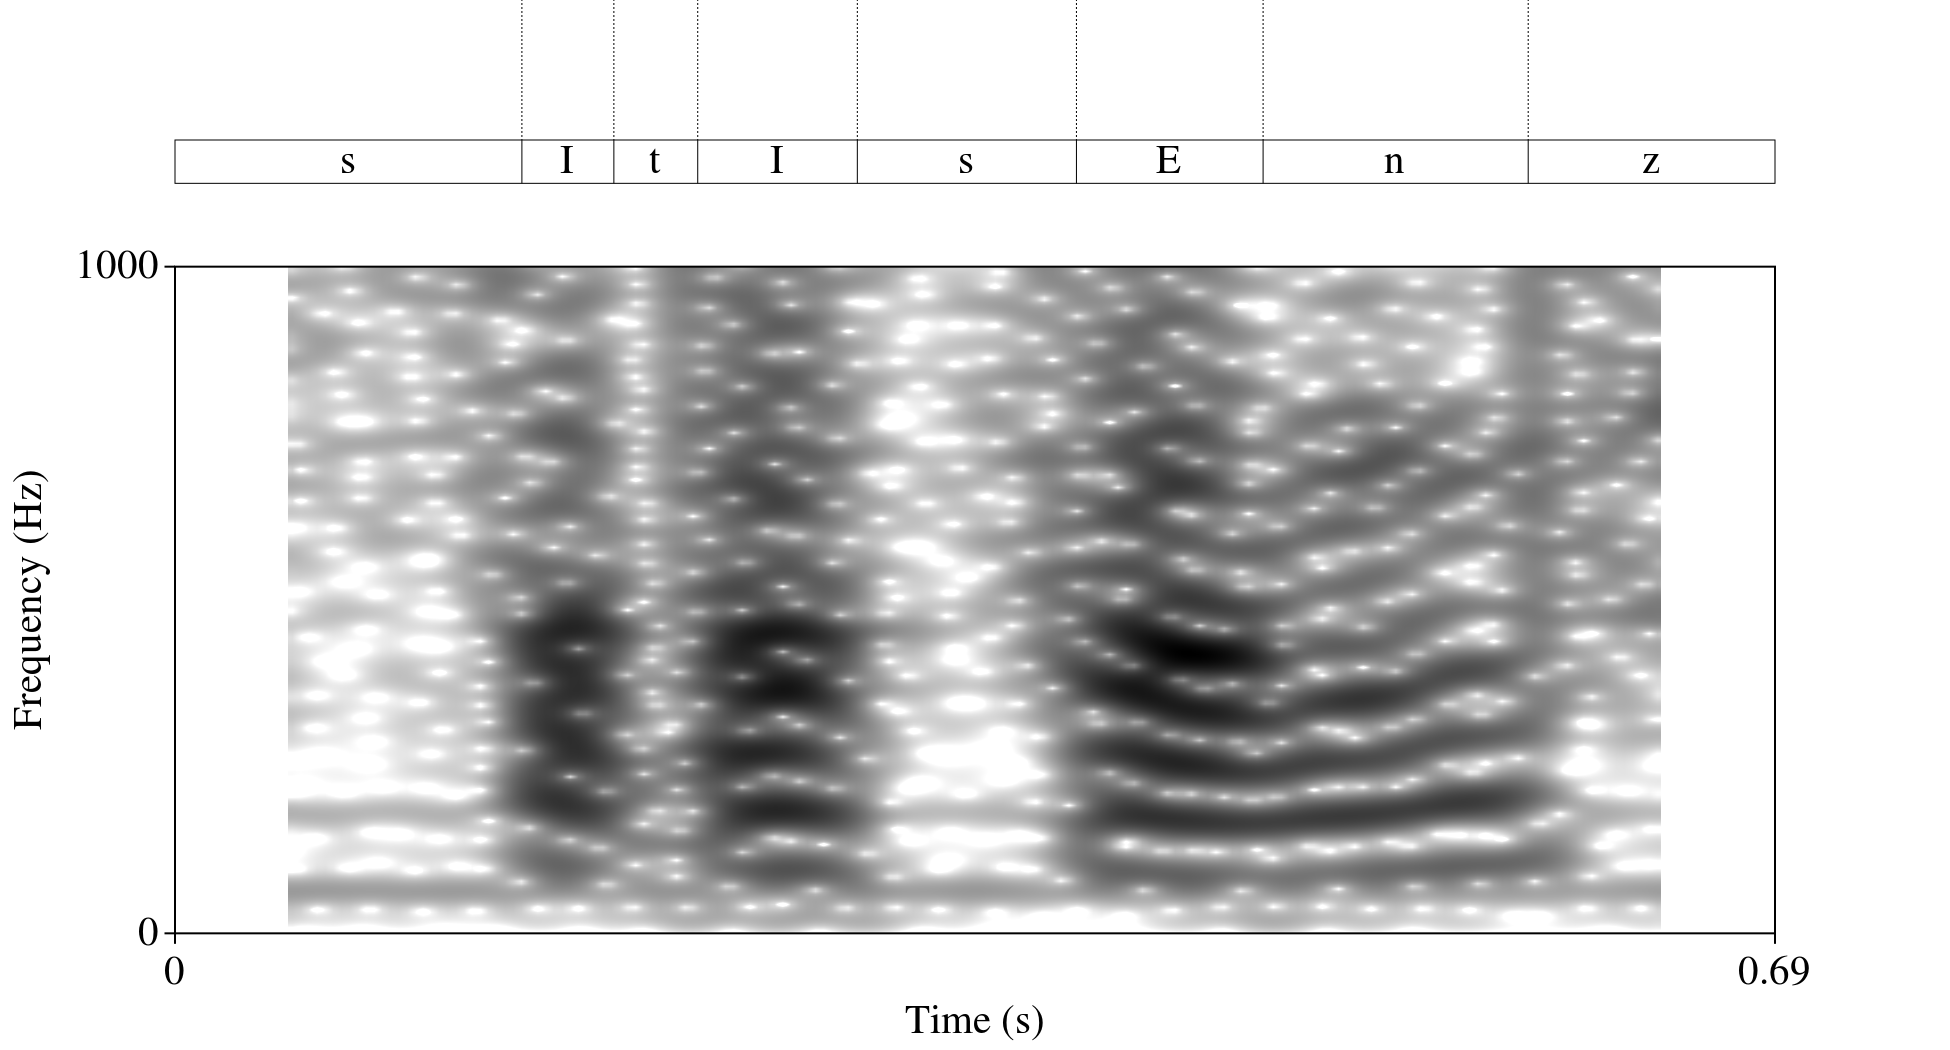
\includegraphics[width=0.95\textwidth]{figure/spctgrm1k.png}
%DIF <    \caption{Zoomed to the 0-1kHz range for better visualization of harmonics.}
%DIF <    \label{fig:spctgrm1k}
%DIF <  \end{subfigure}%
%DIF <  \hfill
%DIF <  \begin{subfigure}{0.95\textwidth}
%DIF <    \centering
%DIF <    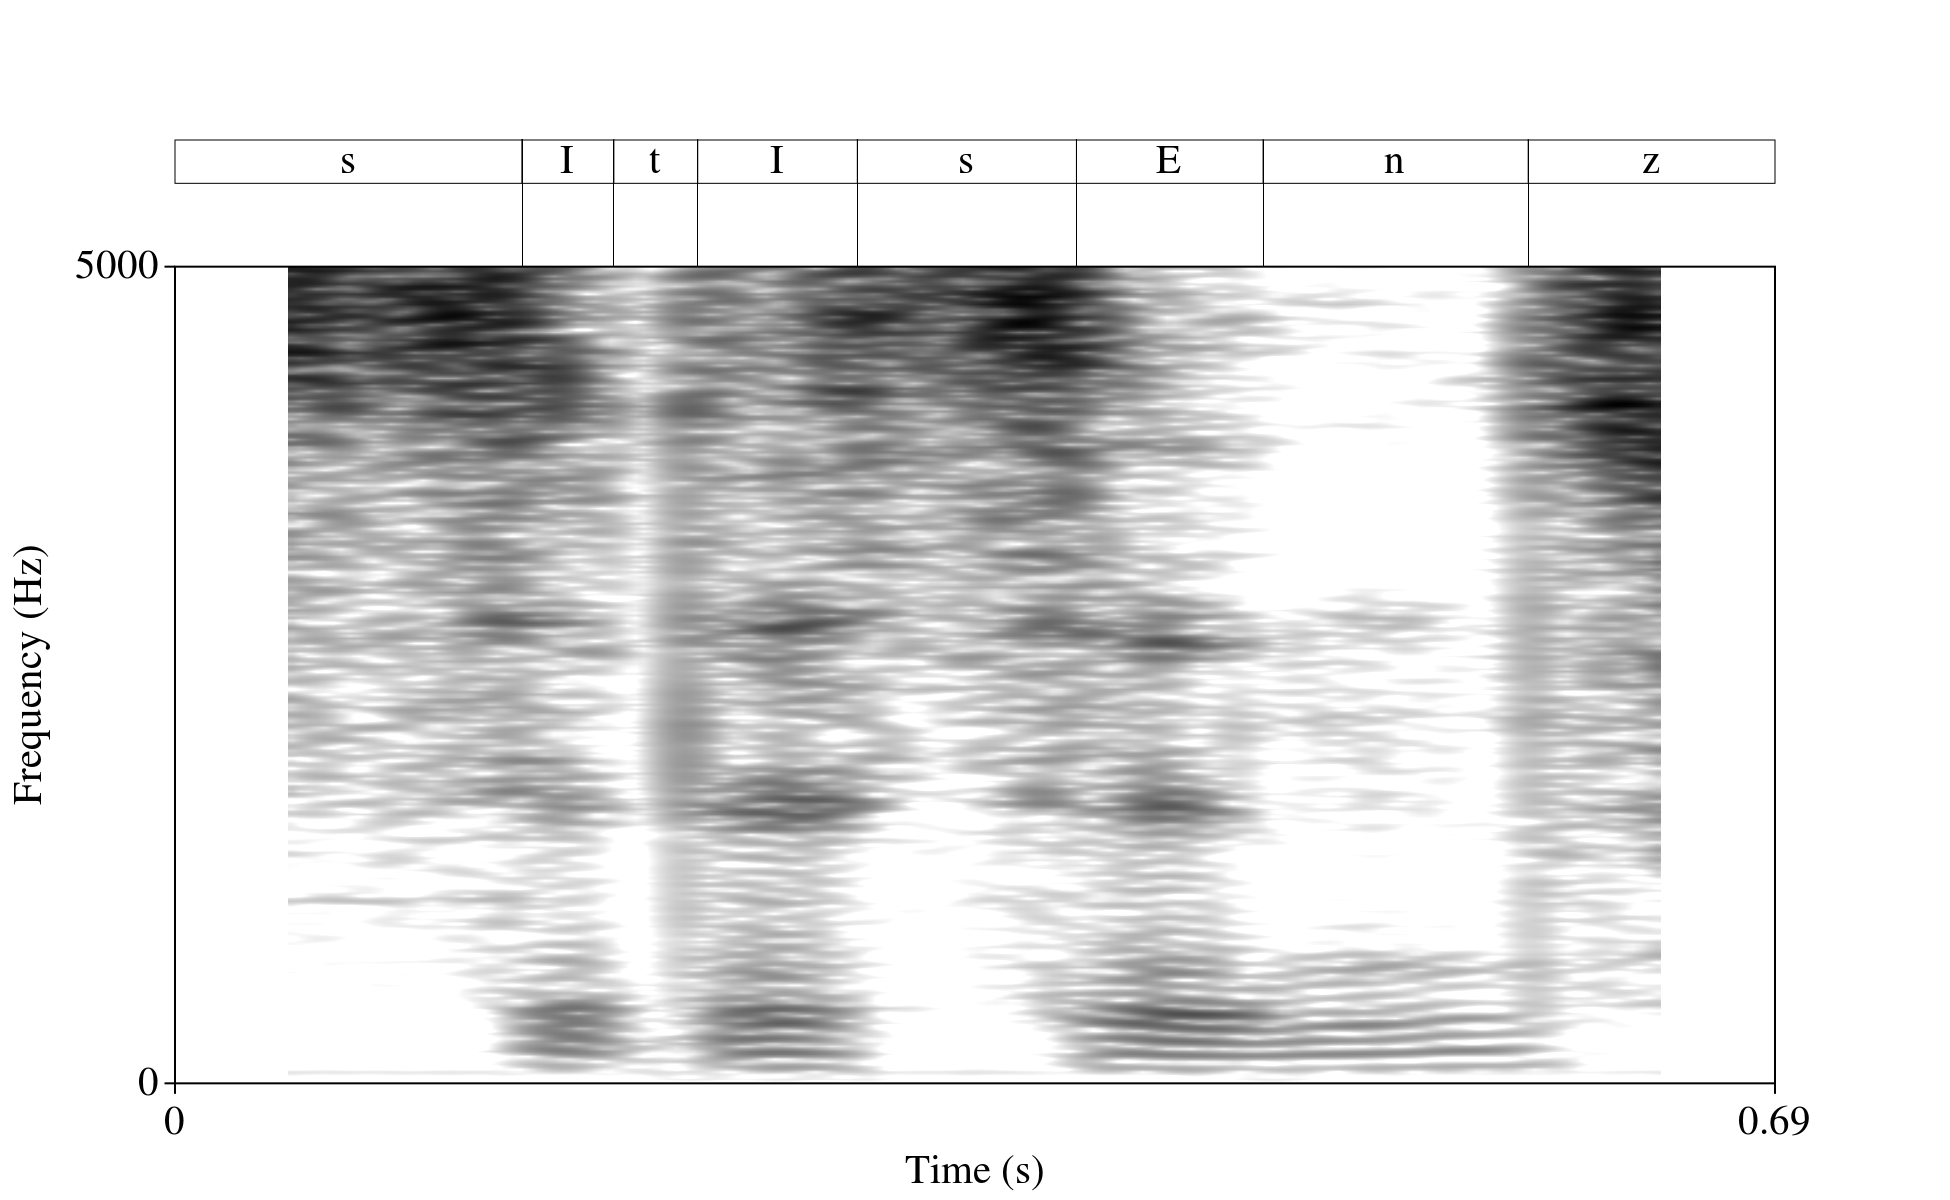
\includegraphics[width=0.95\textwidth]{figure/spctgrm5k.png}
%DIF <    \caption{Zoomed to a more standard 0-5kHz range.}
%DIF <    \label{fig:spctgrm5k}
%DIF <  \end{subfigure}
%DIF <  \caption{Spectrogram of the word ``citizen'' with phonetic transcription above.}
%DIF <  \label{fig:spctgrm1k5k}
%DIF <  \end{figure}
%DIF <  
%DIF <  For unvoiced speech, the information used to recognize and categorize the speech sound is likely found in either the turbulent frication generally centered in higher frequencies cf. fig \ref{fig:spctgrm_s} (although some of the information can be found in lower frequencies), or found in the voiced information in the transitions into and out of the sound (\cite{story:10}).
%DIF <  %
%DIF <  \begin{wrapfigure}{l}{0.5\textwidth}
%DIF <  \centering
%DIF <    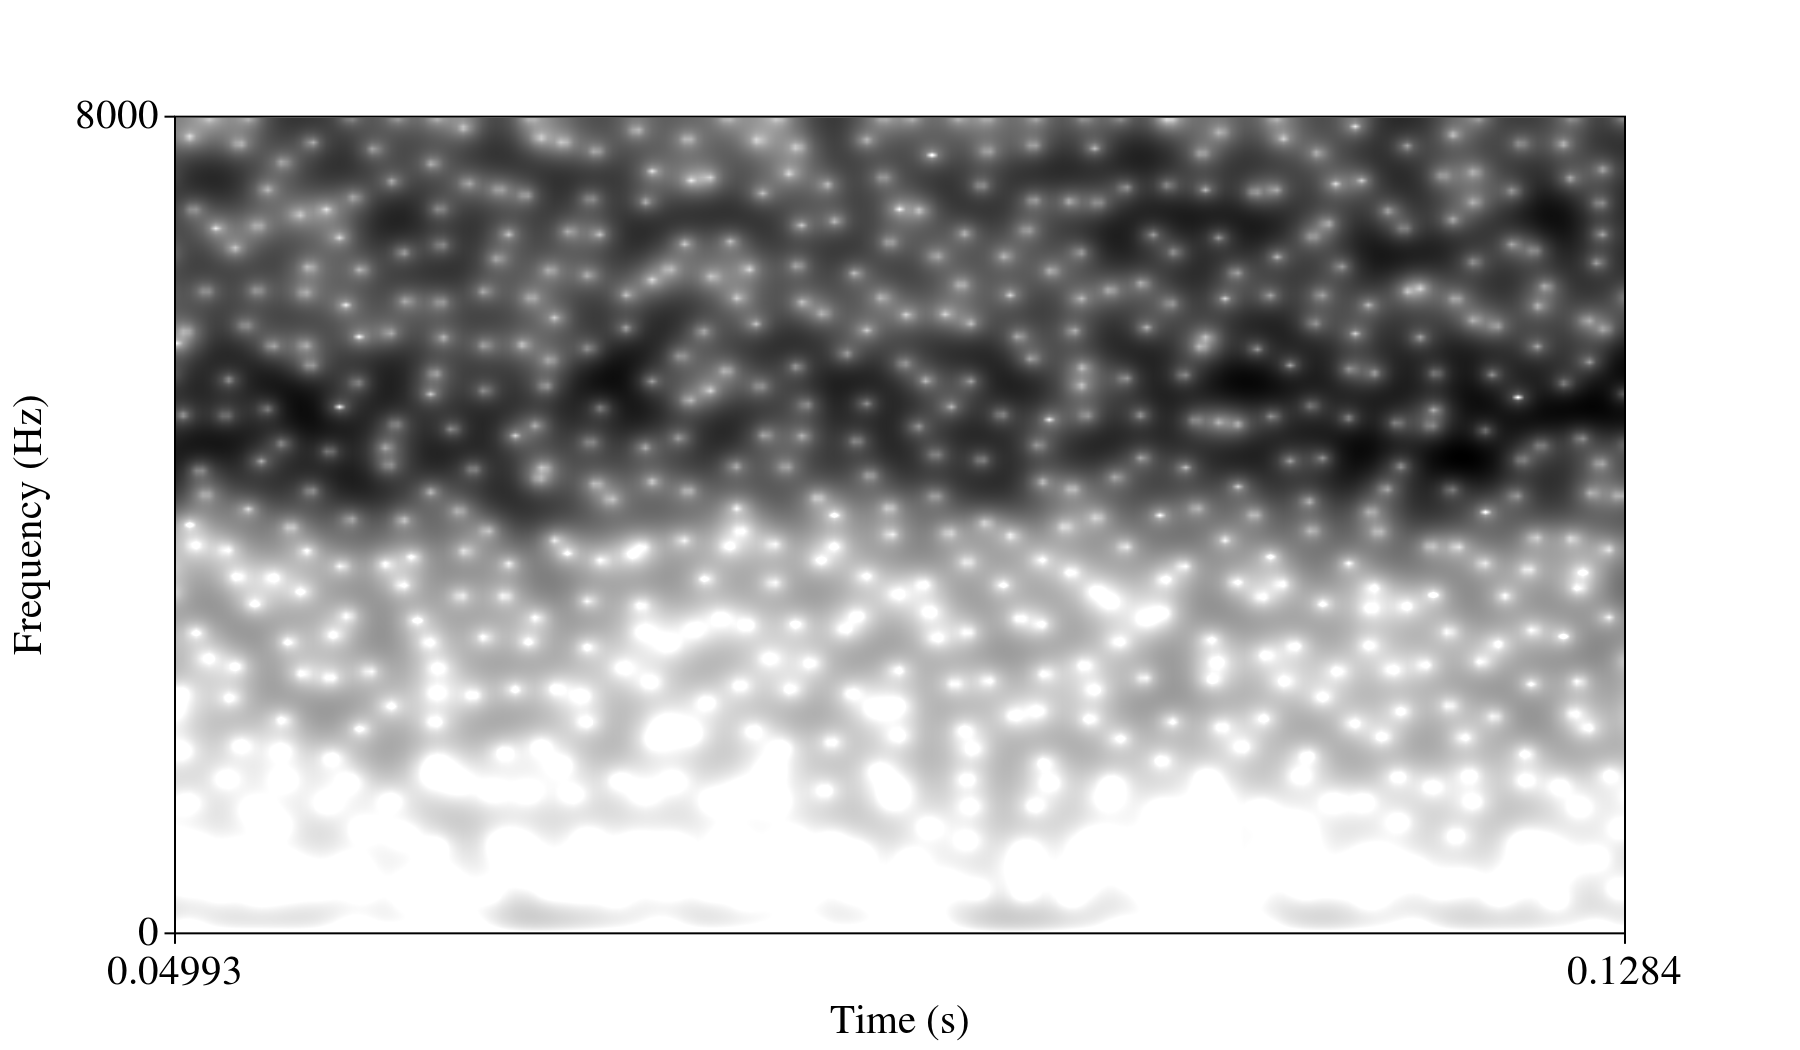
\includegraphics[width=0.5\textwidth]{figure/spctgrm_s.png}
%DIF <    \caption{Spectrum of the initial /s/ in ``citizen''. Zoomed to range of 0-8kHz for visualization of high frequency energy.}
%DIF <    \label{fig:spctgrm_s}
%DIF <  \end{wrapfigure}
\DIFdelbegin %DIFDELCMD < 

%DIFDELCMD < %%%
%DIF <  Discussion about Body/Bone conduction (mechanical)
%DIFDELCMD < \subsection{Bone Conduction}
%DIFDELCMD < %%%
\DIFdelend Bone conduction of acoustic vibrations through a human head has been well studied (cf. \cite{allen:60}, \cite{hakansson:94}, \cite{stenfelt:00}, \cite{reinfeldt:10}, etc); however most of these studies have involved attaching a mechanical vibration device to an animal head or a cadaver skull, or using a vibrating piston on a live human participant, allowing for precise manipulation of the input signal.  
\DIFaddbegin \DIFadd{Many of these early studies mecanical=stimulus studies (most performed on cats or other mammals) do show that the sound generated by bone conduction propagating into the ear canal is dominated by low-frequency noise (\mbox{%DIFAUXCMD
\cite{tonndorf:72}
}%DIFAUXCMD
).
}

\DIFaddend %The acoustic vibrations resulting from the mechanical device positioned on the head propagate to and are recorded by a recording device on a different location on the head.  
% Most of these studies, as well, are focused on audiometric bone conduction, i.e. the propagation of waves through the head and their effect specifically on the cochlea itself, which is not relevant to the present study.
% 
% %One study, \cite{hakansson}, used ``Live'' human subjects .  Titanium implants (pre-existing) for bone-conduction hearing aids anchored in the temporal bone behind the ear were used as the stimulation point for the mechanical vibrators.
% However, some do contain important findings about the general transmission of vibrations through a skull.
%DIF <  Many of the early studies which were performed on cats do show that the sound generated by bone conduction propagating into the ear canal is dominated by low-frequency noise (\cite{tonndorf:72}).  Normally, the open ear acts as a high pass filter, dampening these lower frequencies passing into it via bone conduction.  When occluded, this filter is non existent, and the lower frequencies are more noticeably present (discussed in depth further below). 
%DIF >  Many of these early studies which were performed on cats do show that the sound generated by bone conduction propagating into the ear canal is dominated by low-frequency noise (\cite{tonndorf:72}).  Normally, the open ear acts as a high pass filter, dampening these lower frequencies passing into it via bone conduction.  When occluded, this filter is non existent, and the lower frequencies are more noticeably present (discussed in depth further below). 
%
% Other more recent studies on human subjects have agreed with these findings.  It has also been found that the acoustic response differs significantly depending on the location of the skull that is stimulated\footnote{Typically in these studies it is either the frontal bone or the mastoid process (\cite{bekesy:60}).}.
A few (cf. \cite{bekesy:48}, \cite{hansen:97b}, \cite{porschmann:00}, and \cite{reinfeldt:10}) have investigated bone conduction when the source of vibration (ie. sound) is a person's own voice, not an artificial mechanically-created vibration.  These studies also record \DIFdelbegin \DIFdel{using }\DIFdelend \DIFaddbegin \DIFadd{with }\DIFaddend a microphone at the entrance to a speaker's ear canal, and not via another sensor \DIFdelbegin \DIFdel{on a different side of }\DIFdelend \DIFaddbegin \DIFadd{attached to }\DIFaddend the skull.

The many studies that use a simple mechanically-created vibration as a stimulus do so in part because the use of speech as a source is inherently messy.  This is due to the fact that speech is 
\begin{enumerate*}[label={\alph*)}]
  \item  is not as easily manipulated as a simple mechanically-created vibration,
  \item  contains far more frequency components than a simple mechanically-created vibration, and 
  \item  takes multiple pathways to get to the ear: from the vocal chords, through tissue, and into the ear canal, and also from vibrations in the air all along the vocal tract\footnote{The speech sound is \DIFdelbegin \DIFdel{also }\DIFdelend filtered differently \DIFdelbegin \DIFdel{as it passes }\DIFdelend \DIFaddbegin \DIFadd{at different locations }\DIFaddend along the vocal tract}, through the solid medium of the head\footnote{Although, of course, the head is composed of different tissues with different densities and acoustic resonances}, and back into the medium of air inside the ear canal.
\end{enumerate*}
% 
\DIFdelbegin %DIFDELCMD < \begin{wrapfigure}{l}{0.5\textwidth}
%DIFDELCMD < %%%
%DIF < \begin{figure}
%DIFDELCMD < \centering
%DIFDELCMD <   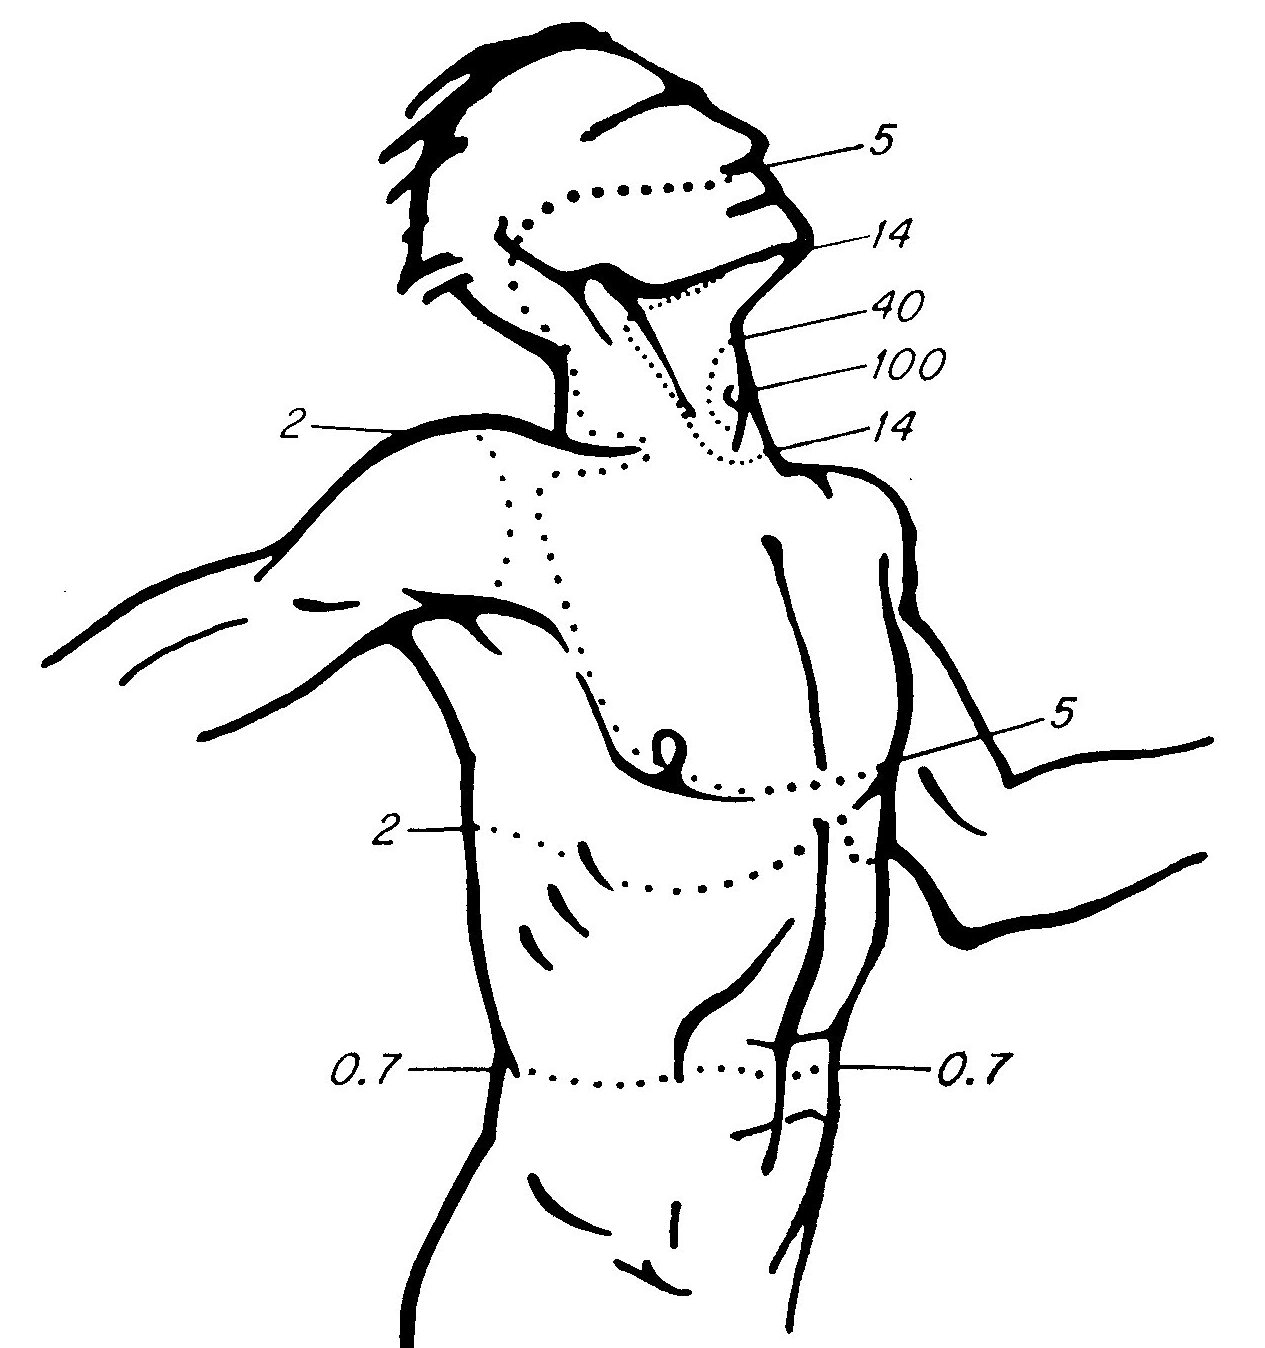
\includegraphics[width=0.5\textwidth]{figure/bekesy60-3b.png}
%DIFDELCMD <   %%%
%DIFDELCMD < \caption{%
{%DIFAUXCMD
\DIFdel{Diagram of the propagation of speech waves throughout the body. Numbers correspond to percentage of the original amplitude of the speech remaining when reaching the marked location. Taken from \mbox{%DIFAUXCMD
\cite{bekesy:60}
}%DIFAUXCMD
.}}
  %DIFAUXCMD
%DIFDELCMD < \label{fig:bekesyBodyTransfer}
%DIFDELCMD < %%%
%DIF < \end{figure}
%DIFDELCMD < \end{wrapfigure}
%DIFDELCMD < %%%
\DIFdelend %DIF >  \begin{wrapfigure}{l}{0.5\textwidth}
%DIF >  %\begin{figure}
%DIF >  \centering
%DIF >    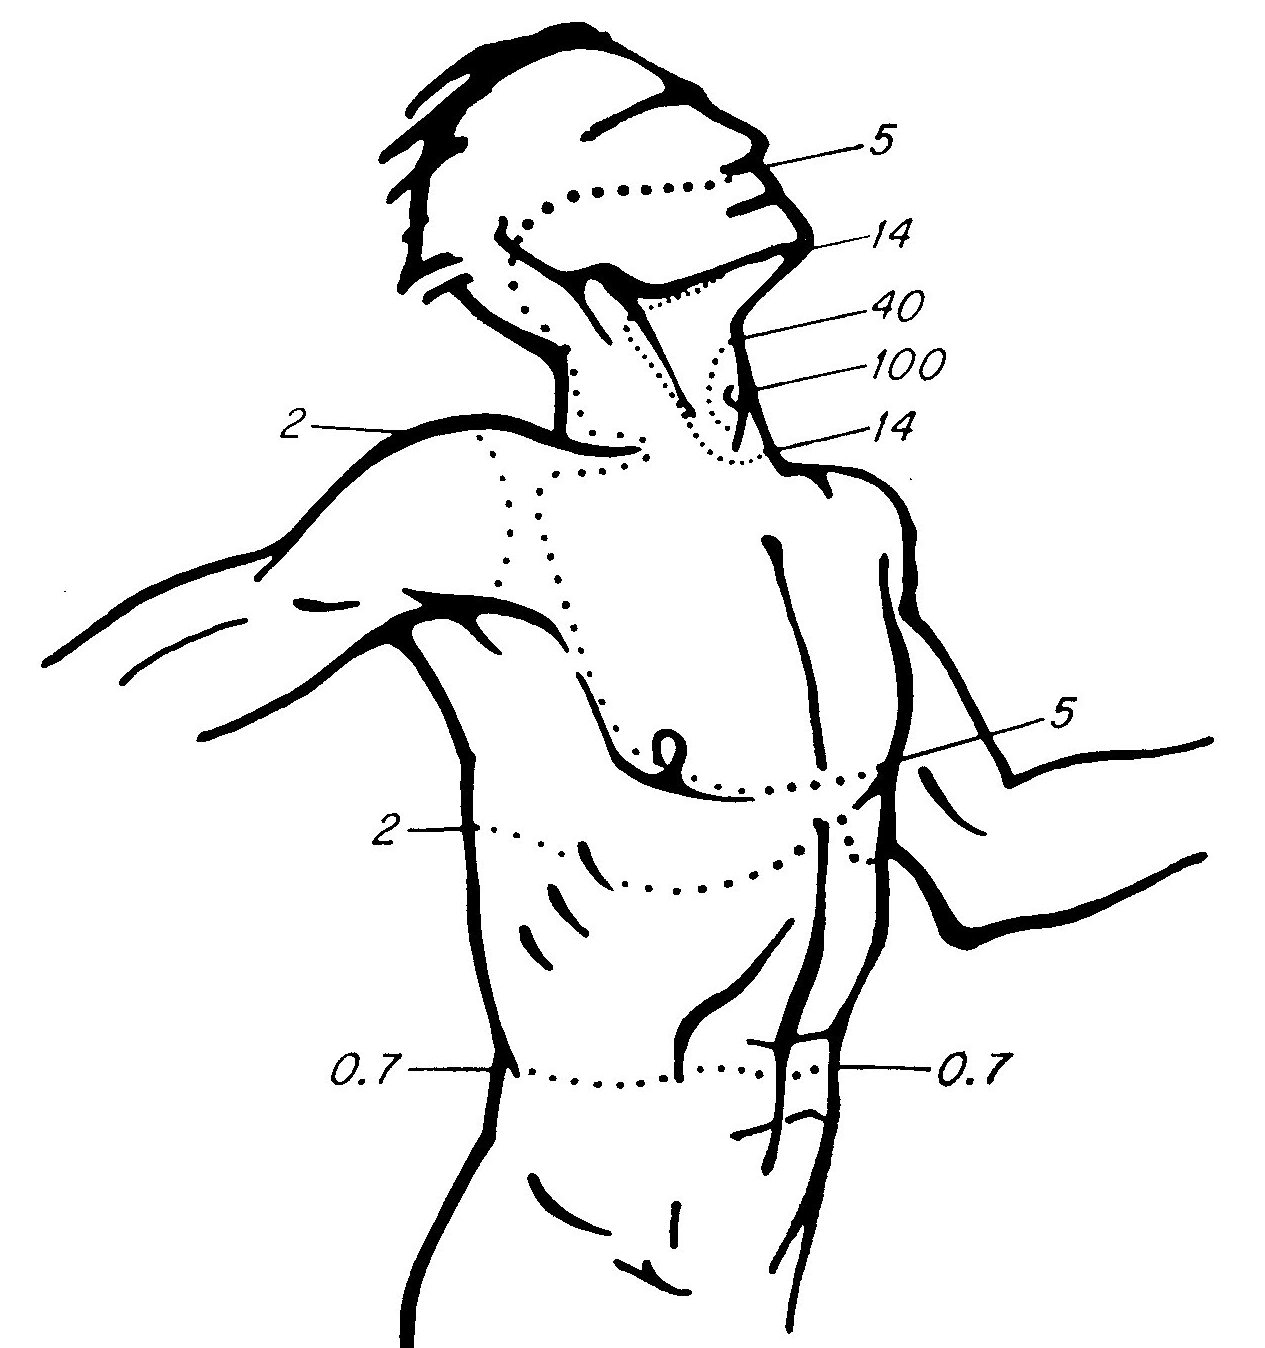
\includegraphics[width=0.5\textwidth]{figure/bekesy60-3b.png}
%DIF >    \caption{Diagram of the propagation of speech waves throughout the body. Numbers correspond to percentage of the original amplitude of the speech remaining when reaching the marked location. Taken from \cite{bekesy:60}.}
%DIF >    \label{fig:bekesyBodyTransfer}
%DIF >  %\end{figure}
%DIF >  \end{wrapfigure}
%
On top of this, the ear canal itself acts as a resonating chamber (\cite{rosen:91}), altering the signal beyond the distortion already caused by the passage through tissue and bone.  


% \subsection{Peripheral Auditory System Anatomy}
% 
% Prior to discussing the resonating characteristics of the ear canal, it is important to become familiar with the basic ear canal anatomy.  The peripheral auditory system is generally grouped into three primary categories, the outer ear, the middle ear, and the inner ear (cf. Figure \ref{fig:ear-anatomy}).  The outer ear includes the pinna, the ear canal tube, and the tympanic membrane (ie. the eardrum).  Air-transmitted vibrations (sound) enter the ear canal through the opening at the pinna.  These then travel along the canal to vibrate the tympanic membrane, which passes the energy to the middle ear.  The middle ear includes the ossicles within the middle ear cavity.  These are a series of very small bones that the vibrational energy travels along, until it is passed into the cochlea in the inner ear.
% 
% The inner ear is composed of the cochlea, the semicircular canals (and vestibule), and the auditory and vestibular nerves.  The semicircular canals, vestibule, and vestibular nerve don't play a part in audition (their primary function regards balance sensitivity).  The cochlea receives the vibrations passed along through the middle ear ossicles.  These vibrations travel through a fluid substance in the cochlea, are sensed by hair cells within the cochlea, and transmitted as electrical pulses to the auditory nerve.
% 
% \begin{figure}[h]
% \centering
%   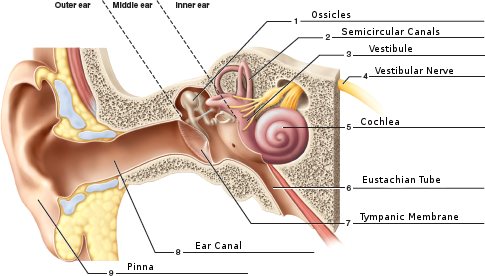
\includegraphics{figure/ear_anatomy.png}
%   \caption{A diagram of the peripheral auditory system, including the outer ear, middle ear, and inner ear, up to the auditory nerve. (Image from \cite{martin:12})}
%   \label{fig:ear-anatomy}
% \end{figure}
% 
% Of interest to this present study is the outer ear.  Typically, as described above, vibrations will enter the ear canal through the opening at the pinna.  However, vibrations from one's own speech are also transmitted via the bone, cartilage, and tissue of the head.  Regardless of source, sound vibrations entering into the ear canal will be altered by the shape of the ear canal, described more below.

% Discussion about EAC resonance Theory
\DIFdelbegin %DIFDELCMD < \subsection{Ear Canal Resonance}
%DIFDELCMD < %%%
\DIFdelend \DIFaddbegin \subsection{Modelling Ear Canal Resonance}
\DIFaddend % \begingroup
\DIFdelbegin \DIFdel{There has been much research on }\DIFdelend \DIFaddbegin \DIFadd{We've discussed that a speech signal can reach the ear canal by passing through bone and tissue.  This section will describe what happens to the signal when it reaches the ear canal. 
}

\DIFadd{There have been many investigations of }\DIFaddend the resonating characteristics and amplitude response of the ear canal.  One such project was performed by \cite{stinson:89}, which studied fifteen human ear canals.  Their aim was to produce a model which could replicate the effect that the ear canal has on acoustics.
One challenge in producing such a model is the considerable variability in the shape of the canal - both between subjects as well as between the right and left ear canal of a single subject (\cite{stinson:89}).  These differences are apparent in curvature, length, volume, and cross-sectional diameter throughout the ear canal.  \cite{stinson:89} created silicon ear molds for each of the ear canals, which were used to generate three different computational models: one following the contours and dimensions of their ear molds exactly, another following the dimensions of the ear mold, but straightening contours and curvatures as if along a central axis, and the third as if the ear canal were a uniform tube with the same length and volume of the ear canal molds and previous models (see Fig. \ref{fig:eac_modelling}).  They noted that most significant differences between these models' spectral predictions of ear canal resonance occur above 6kHz.

%
\begin{figure}[h!]
% \begin{wrapfigure}{L}{0.5\textwidth}
\centering
  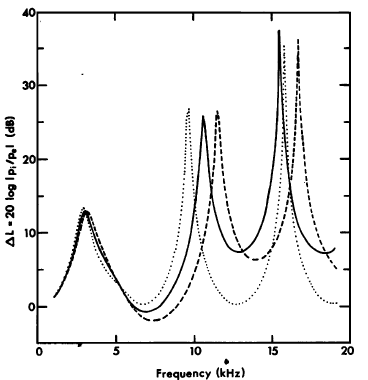
\includegraphics[width=0.4\textwidth]{figure/eac_mod_diffs.png}
  \caption{\cite{stinson:89} diagrams three different models of the ear canal resonance.  The bold line is based on their 3D canal molds from cadavers, the dashed line removes the curvature of the ear canal and acts as if the axis were straight, the dotted line assumes a constant diameter along a straight axis, with the same ear canal volume as the dashed and solid lines.}
  \label{fig:eac_modelling}
% \end{wrapfigure}
\end{figure}
%

\DIFdelbegin \DIFdel{Since much of the acoustic information for distinguishing speech sounds is located below 6kHz, several (cf. \mbox{%DIFAUXCMD
\cite{stinson:89,hansen:97b,stenfelt:07}
}%DIFAUXCMD
) who have made efforts to model the ear canal, have chosen to simply treat it as if it were a uniform tube.  Treating the ear canal model as a uniform tube, as opposed to incorporating the nuances of its diameter and curvature, will not have much effect on the output of a model.
}%DIFDELCMD < 

%DIFDELCMD < %%%
\DIFdelend Another challenge is to obtain the dimensions of the ear canal needed in order to treat it as a uniform tube\DIFaddbegin \DIFadd{, ie the length and diameter}\DIFaddend . Immittance measurements are widely used in audiology, and involve emitting a chirp or tone into a pressurized ear canal.  The chirp then bounces back from the tympanic membrane (assumed to have infinite impedance in a pressurized canal) and can be recorded (\cite{ballachanda:97}, 415): ``The sound pressure developed inside a rigid cavity from a known sound source is directly related to the volume of the cavity".  Therefore, the volume of the ear canal can be inferred for a subject using immittance testing without the need for invasive measurements (eg. using a silicon mold).  Making an assumption about either an `average' diameter or an `average' length of the ear canal would allow for the approximate calculation of the other dimension, given the measured volume. The average length of the ear canal has been cited from \DIFdelbegin \DIFdel{23mm }\DIFdelend \DIFaddbegin \DIFadd{23 mm }\DIFaddend (\cite{rosen:91}) up to approximately \DIFdelbegin \DIFdel{29mm }\DIFdelend \DIFaddbegin \DIFadd{29 mm }\DIFaddend (\cite{stinson:89}) for a straight tube. The average diameter for the ear canal is approximately 7.1 mm (\cite{salvinelli:91}).
%These ear canal dimensions can then be plugged into any one of several models designed to approximate the ear canal dimensions.

\DIFdelbegin %DIFDELCMD < \begin{figure}[h!]
%DIFDELCMD < \centering
%DIFDELCMD <   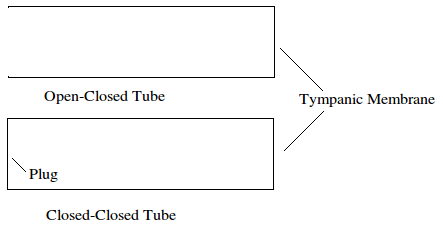
\includegraphics{figure/open-closed-tube.png}
%DIFDELCMD <   %%%
%DIFDELCMD < \caption{%
{%DIFAUXCMD
\DIFdel{A diagram showing an example of an open-closed tube (top) and a closed-closed tube (bottom).  Applied to the case at hand, the closed end (on the right) in both figures would be the tympanic membrane.  The opening at the left (top) is the entrance to the ear canal, which can be plugged (bottom).}}
  %DIFAUXCMD
%DIFDELCMD < \label{fig:open-closed-tube}
%DIFDELCMD < \end{figure}
%DIFDELCMD < 

%DIFDELCMD < %%%
\DIFdel{Once inside }\DIFdelend \DIFaddbegin \DIFadd{Since much of the acoustic information for distinguishing speech sounds is located below 6 kHz, and the various resonance models developed by \mbox{%DIFAUXCMD
\cite{stinson:89}
}%DIFAUXCMD
are very similar below 6 kHz, several (cf. \mbox{%DIFAUXCMD
\cite{stinson:89,hansen:97b,stenfelt:07}
}%DIFAUXCMD
) who have made efforts to model }\DIFaddend the ear canal\DIFdelbegin \DIFdel{with known approximate dimensions, it can either be modeled }\DIFdelend \DIFaddbegin \DIFadd{, have chosen to simply treat it as if it were a uniform tube.  Treating the ear canal model }\DIFaddend as a uniform tube\DIFdelbegin \DIFdel{.  }\DIFdelend \DIFaddbegin \DIFadd{, as opposed to incorporating the nuances of its diameter and curvature, will not have much effect on the output of a model, and greatly simplifies the calcultions.
}

\begin{figure}[h!]
\centering
  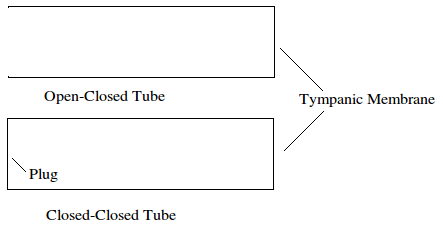
\includegraphics{figure/open-closed-tube.png}
  \caption{\DIFaddFL{A diagram showing an example of an open-closed tube (top) and a closed-closed tube (bottom).  Applied to the case at hand, the closed end (on the right) in both figures would be the tympanic membrane.  The opening at the left (top) is the entrance to the ear canal, which can be plugged (bottom).}}
  \label{fig:open-closed-tube}
\end{figure}

\DIFaddend The acoustics of uniform tubes is usually thought of in terms of an open-open tube, an open-closed tube, or a closed-closed tube.  Each of these have different resonating characteristics. The human vocal tract, for example, is normally modeled as an open-closed tube, where one end (the glottis) is generally considered `closed' for modelling purposes, and the other (the mouth) is generally considered to be `open'.  Similarly, for the human ear, the tympanic membrane represents the `closed' end of the ear canal tube, and the ear canal opening at the concha, or pinna, is the `open' end (cf. Figure \ref{fig:open-closed-tube}).  It can also be modeled as a closed-closed tube if the ear is plugged (cf. Figure \ref{fig:open-closed-tube}). This difference changes the resonance and reverberant structure of the ear canal, and will be discussed further in Section \ref{sec:OEBCspeech}.  

%BC+EC-OE
\DIFdelbegin %DIFDELCMD < \subsection{Ear Canal Resonance on Bone-Conducted Speech}
%DIFDELCMD < %%%
\DIFdelend %DIF >  \subsection{Ear Canal Resonance on Bone-Conducted Speech}

\DIFdelbegin \DIFdel{There have been many studies pertaining to ear canal resonance from bone conducted speech. There }\DIFdelend \DIFaddbegin \DIFadd{The resonances of ear canal can be modeled as if the canal were a uniform tube, without much loss in accuracy.  This has been determined by modelling tones at different frequencies emanating from the entrance of the ear, recorded at the tympanic membrane, and noting the change in resonant frequency. However, there }\DIFaddend are a few \DIFdelbegin \DIFdel{in particular }\DIFdelend (c.f. \cite{bekesy:48}, \cite{porschmann:00}, \cite{reinfeldt:10}) who use real human speech as the sound source\DIFaddbegin \DIFadd{, and bone-conduction as the medium.  This would result is speech }\textit{\DIFadd{not}} \DIFadd{emitted at the entrance to the ear canal, but entering the ear canal through the ear canal walls}\DIFaddend .
%
% The acoustics of uniform tubes is usually thought of in terms of an open-open tube, an open-closed tube, or a closed-closed tube.  Each of these have different resonating characteristics. The human vocal tract, for example, is normally modeled as an open-closed tube, where one end (the glottis) is generally considered `closed' for modelling purposes, and the other (the mouth) is generally considered to be `open'.  Similarly, for the human ear, the tympanic membrane represents the `closed' end of the ear canal tube, and the ear canal opening at the concha, or pinna, is the `open' end (cf. Figure \ref{fig:open-closed-tube}).

\cite{porschmann:00}'s study is generally looking at the \textit{self-perception} of one's own voice, but in order to accomplish this devotes effort to looking at the bone conduction pathway separately.  A general 0.9 kHz resonance (with subsequent harmonic resonances) was found in the collected bone-conduction speech, \DIFdelbegin \DIFdel{with the amplitude gain }\DIFdelend generally present between 0.7 and 1.2 kHz.  This correlates with the 0.8-1.2 kHz range for the first resonance that others (cf. \cite{hakansson:94}) have observed in mechanical-stimulated bone conduction studies. This would mean, in terms of speech, that one would expect to find higher \DIFaddbegin \DIFadd{relative }\DIFaddend amplitudes near the first formant.

However, in this study only two phones were used (/s/ and /z/), and a masking threshold\footnote{The masking threshold technique involves playing a pure tone at different frequencies and amplitudes while the participant is phonating. The participant indicates when the tone becomes audible over their own speech. Knowing the amplitude of the tone allows the researcher to know the amplitude of the speech as one becomes audible over the other. Having this knowledge, the spectrum of speech as it is perceived by the speaker can to be mapped.} technique was used to determine the frequency spectrum of the transfer function of body conduction.  This is admittedly a rather subjective method of determining the spectrum.  

\cite{reinfeldt:10}, \DIFdelbegin \DIFdel{on the other hand, }\DIFdelend use microphones to record the actual sound pressure level (SPL) of both air- and body-conducted speech. Furthermore, \cite{reinfeldt:10} used a more \DIFdelbegin \DIFdel{expansive and }\DIFdelend diverse set of phones.  \DIFdelbegin \DIFdel{While a }\DIFdelend \DIFaddbegin \DIFadd{A }\DIFaddend resonance was found in generally the same frequency region for /s/ (and other phones) as that found by \cite{porschmann:00} (0.7 - 1.2 kHz) \DIFdelbegin \DIFdel{, they discovered some distinct differences, which can be seen in Fig. \ref{BCrelAC}. }\DIFdelend \DIFaddbegin \DIFadd{and \mbox{%DIFAUXCMD
\cite{hakansson:94}
}%DIFAUXCMD
(0.8 - 1.2 kHz). %DIF > , they discovered some distinct differences, which can be seen in Fig. \ref{BCrelAC}. 
}\DIFaddend Between each class that was used - voiceless sounds (/s/, /t/, /k/, and /tj/),  nasals (/m/ and /n/), and vowels (/i/, /e/, /a/, /o/) - a moderately similar frequency response is seen, yet there are some distinctions to note\DIFdelbegin \DIFdel{(see Fig. \ref{BCrelACall}). }\DIFdelend \DIFaddbegin \DIFadd{. %DIF > (see Fig. \ref{BCrelACall}).
}\DIFaddend 

In particular, \DIFdelbegin \DIFdel{as can be seen in Fig. \ref{BCrelAC}, }\DIFdelend %DIF > as can be seen in Fig. \ref{BCrelAC}, 
there is much inter-speaker variation within the body conduction of the same sound.  \DIFdelbegin \DIFdel{While it is difficult to track an individual speaker's relative spectral envelope within the figure, it }\DIFdelend %DIF > While it is difficult to track an individual speaker's relative spectral envelope within the figure, 
\DIFaddbegin \DIFadd{It }\DIFaddend appears that much of this difference, particularly in the lower frequencies, originates from a difference in amplitude, and not necessarily from different resonance locations along the frequency axis.  \DIFdelbegin \DIFdel{It is important to note that both Figs. \ref{BCrelAC} and \ref{BCrelACall} both contain }\textit{\DIFdel{relative}} %DIFAUXCMD
\DIFdel{spectral envelopes - ie. the difference between the air-conducted and body-conducted components of speech, and do not contain an absolute frequency spectrum of body-conducted speech. 
}\DIFdelend %DIF > It is important to note that both Figs. \ref{BCrelAC} and \ref{BCrelACall} both contain \textit{relative} spectral envelopes - ie. the difference between the air-conducted and body-conducted components of speech, and do not contain an absolute frequency spectrum of body-conducted speech. 

Another distinction is that the /e/ vowel has a relatively flat response up to 500 Hz, and dips down to -5 dB around 1kHz.  This is in contrast with the phone /s/, which has a fairly high (yet falling) response below 500 Hz, and does not dip below -5 dB until nearly 4 kHz.  Compared with /e/, the body-conducted to air-conducted ratio for /s/ has a significant downward slope after 2000 Hz.  This is likely due to the fact that there is relatively little energy produced by /s/ in the low frequencies, allowing for a high ratio, which drops as the general energy of the phone increases.  This could indicate that most of the energy produced by a obstruent does not pass through to the ear canal (\cite{reinfeldt:10}).

\DIFdelbegin %DIFDELCMD < \begin{figure}[h!]
%DIFDELCMD < 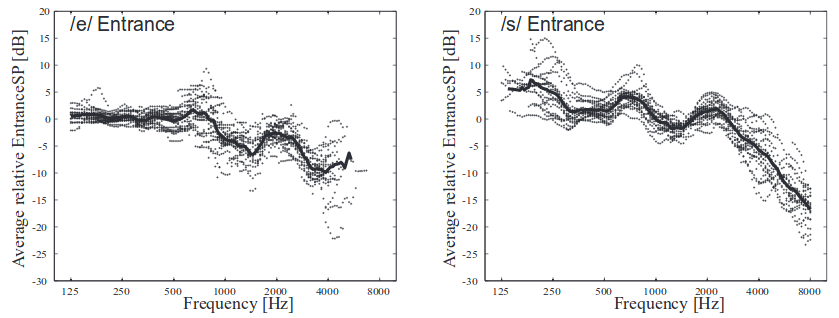
\includegraphics[width=1\textwidth]{figure/BCrelAC_e_s.png}
%DIFDELCMD < %%%
%DIFDELCMD < \caption{%
{%DIFAUXCMD
\DIFdel{The amplitude of Body-Conducted speech relative to the amplitude of Air-Conducted  speech as recorded in the ear canal for the phones /e/ and /s/.  A value of less than zero indicates the amplitude of body-conducted speech is less than that of air-conducted speech, and a value greater than zero indicates a higher amplitude of body-conducted speech than air-conducted speech. The solid line indicates the mean, and the remaining data points are from individual speakers.  The signal was measured from the entrance of an open ear canal.  Taken from \mbox{%DIFAUXCMD
\cite{reinfeldt:10}
}%DIFAUXCMD
.}}
%DIFAUXCMD
%DIFDELCMD < \label{BCrelAC}
%DIFDELCMD < \end{figure}
%DIFDELCMD < %%%
\DIFdelend %DIF >  \begin{figure}[h!]
%DIF >  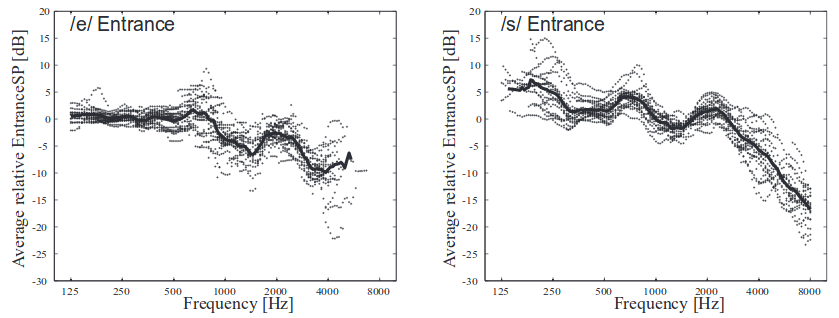
\includegraphics[width=1\textwidth]{figure/BCrelAC_e_s.png}
%DIF >  \caption{The amplitude of Body-Conducted speech relative to the amplitude of Air-Conducted  speech as recorded in the ear canal for the phones /e/ and /s/.  A value of less than zero indicates the amplitude of body-conducted speech is less than that of air-conducted speech, and a value greater than zero indicates a higher amplitude of body-conducted speech than air-conducted speech. The solid line indicates the mean, and the remaining data points are from individual speakers.  The signal was measured from the entrance of an open ear canal.  Taken from \cite{reinfeldt:10}.}
%DIF >  \label{BCrelAC}
%DIF >  \end{figure}

More specific dichotomies can be found between sounds within the same class. For example, the low vowel /a/ is pronounced with a more open mouth vs the relatively closed mouth of the high vowel /i/; consequently, the body-conducted amplitude relative to the air-conducted counterpart was much higher for /i/ than it was for /a/. An assumption could be made from the data that the more open the mouth is, the more energy is transferred to the air-conducted signal\DIFdelbegin \DIFdel{(cf. Fig. \ref{BCrelACall}).}\DIFdelend \DIFaddbegin \DIFadd{.%DIF >  (cf. Fig. \ref{BCrelACall}). 
}\DIFaddend \cite{reinfeldt:10}'s findings are backed by \cite{bekesy:60}, who also \DIFdelbegin \DIFdel{diagrammed }\DIFdelend \DIFaddbegin \DIFadd{noted %DIF > diagrammed 
}\DIFaddend the relative difference in amplitude in the ear canal between the air-conduction and body-conduction of vowels\DIFdelbegin \DIFdel{(cf. Fig. \ref{bekesyPhoneDiff}), }\DIFdelend \DIFaddbegin \DIFadd{, %DIF > (cf. Fig. \ref{bekesyPhoneDiff}), 
}\DIFaddend which also supports this hypothesis.  There was much inter-speaker variability in the previous studies, but the bone-conducted vowels appeared to have the least relative reduction in amplitude are the higher vowels.  Since the functions of other high sonorants (eg. /u/) are not given, we cannot be certain if this is a phone-specific difference, or if it can be generalized to other \DIFdelbegin \DIFdel{sound }\DIFdelend \DIFaddbegin \DIFadd{sounds }\DIFaddend with a [high] articulation in which the tongue is close to the roof of the mouth.  This latter generalization would make sense, as the oral cavity is more `closed\DIFaddbegin \DIFadd{'}\DIFaddend , trapping energy inside the cavity resulting in \DIFdelbegin \DIFdel{move }\DIFdelend \DIFaddbegin \DIFadd{more }\DIFaddend reverberations passing through the head and into the ear canal.
%
\DIFdelbegin %DIFDELCMD < \begin{wrapfigure}{l!}{0.5\textwidth}
%DIFDELCMD < %%%
%DIF <  \begin{figure}
%DIFDELCMD < 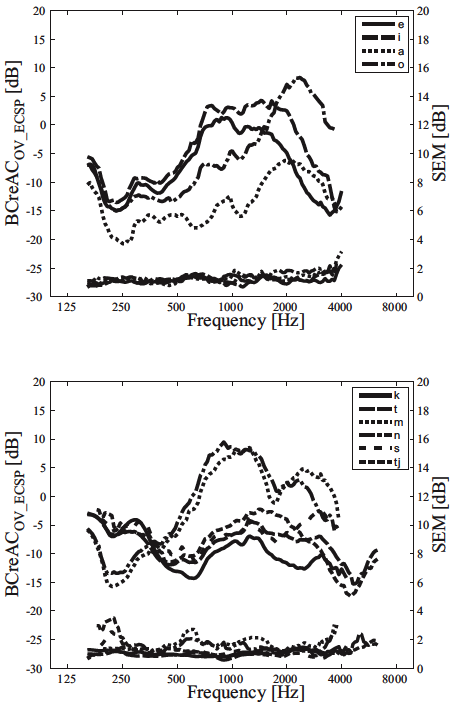
\includegraphics[width=0.45\textwidth]{figure/BC_rel_AC_all.png}
%DIFDELCMD < %%%
%DIFDELCMD < \caption{%
{%DIFAUXCMD
\DIFdel{The mean relative amplitudes (left ordinate) of body conduction relative to air conduction for vowels (top plot) and other sounds (bottom plot).  The set of lines along the bottom of each plot represent the standard error from the mean (SEM), measure on the right ordinate.  Taken from \mbox{%DIFAUXCMD
\cite{reinfeldt:10}
}%DIFAUXCMD
.}}
%DIFAUXCMD
%DIFDELCMD < \label{BCrelACall}
%DIFDELCMD < %%%
%DIF <  \end{figure}
%DIFDELCMD < \end{wrapfigure}
%DIFDELCMD < %%%
\DIFdelend %DIF >  \begin{wrapfigure}{l!}{0.5\textwidth}
%DIF >  % \begin{figure}
%DIF >  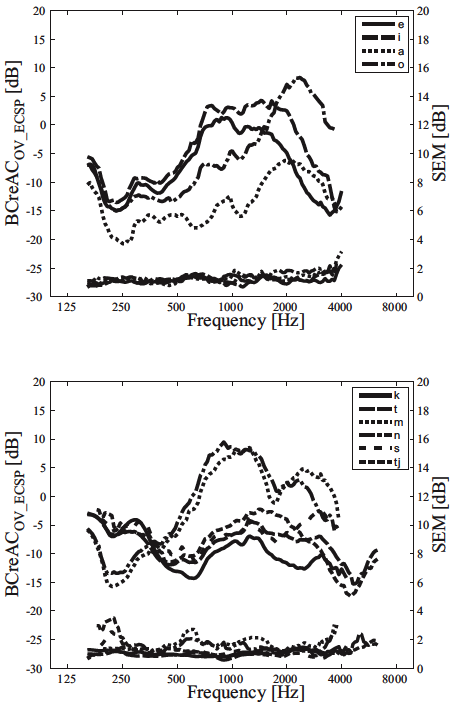
\includegraphics[width=0.45\textwidth]{figure/BC_rel_AC_all.png}
%DIF >  \caption{The mean relative amplitudes (left ordinate) of body conduction relative to air conduction for vowels (top plot) and other sounds (bottom plot).  The set of lines along the bottom of each plot represent the standard error from the mean (SEM), measure on the right ordinate.  Taken from \cite{reinfeldt:10}.}
%DIF >  \label{BCrelACall}
%DIF >  % \end{figure}
%DIF >  \end{wrapfigure}
%
On the surface, it appears that the more energy that is lost to air conduction during the production of low vowels (ie. from a more `open' articulation), the less energy is transferred into the surrounding tissue.
%\footnote{\cite{bekesy:60} does not break down relative amplitude by frequency.}

Here it is important to re-emphasize that these transforms are given as body-conducted amplitude \textit{relative to} air-conducted amplitude for the given phone, and do not reflect the absolute air- and body-conducted amplitude of phones compared with one another.  For example, /a/ is a relatively loud air-conducted sound due to its open articulation, and this loud air-conducted component may cause its \textit{relative} body-conducted component to appear quieter than the other vowels, when in reality it is possible that the body-conducted component of both vowels have the same absolute amplitude.  Neither \cite{bekesy:60} nor \cite{reinfeldt:10} give information about body-conducted components in relation to one another, and so a direct comparison between two bone-conducted phones cannot be conducted.

\DIFdelbegin %DIFDELCMD < \begin{wrapfigure}{R}{0.5\textwidth}
%DIFDELCMD < 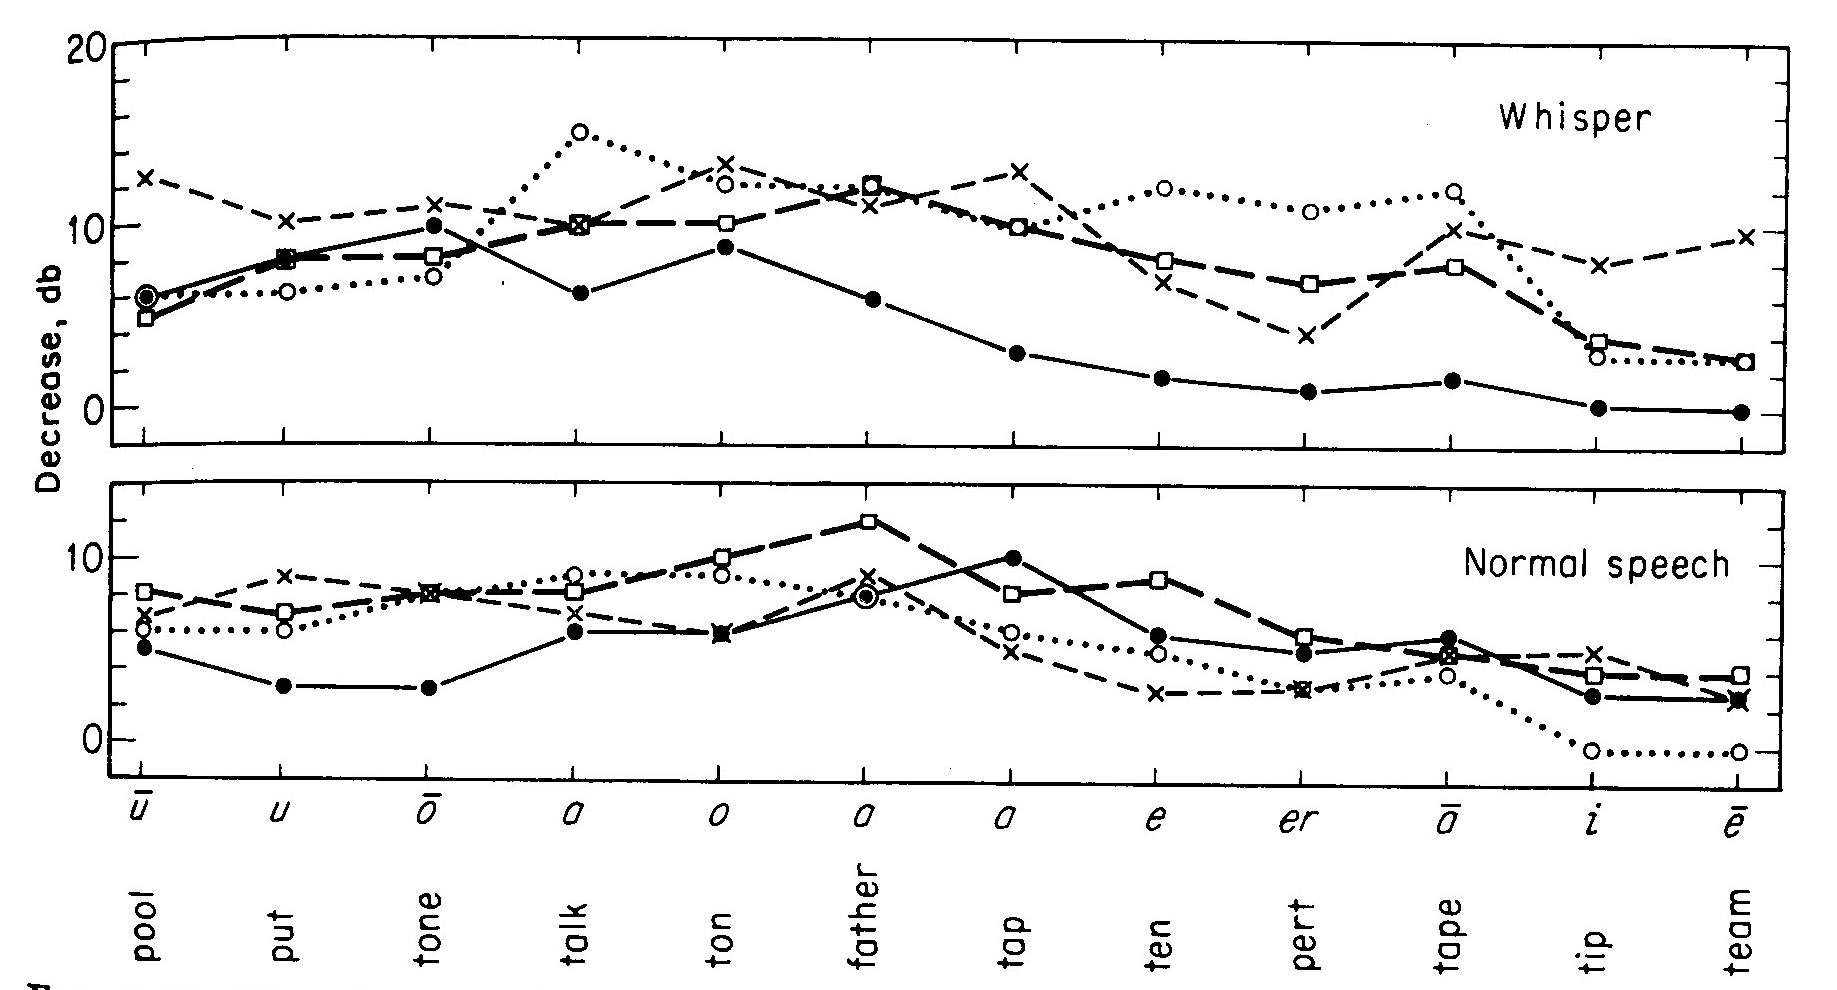
\includegraphics[width=0.5\textwidth]{figure/bekesy60-3.png}
%DIFDELCMD < %%%
%DIFDELCMD < \caption{%
{%DIFAUXCMD
\DIFdel{Demonstrated the different effect on amplitude that closing the ear canal has on the different vowels of English.  Taken from \mbox{%DIFAUXCMD
\cite{bekesy:60}
}%DIFAUXCMD
.}}
%DIFAUXCMD
%DIFDELCMD < \label{bekesyPhoneDiff}
%DIFDELCMD < \end{wrapfigure}
%DIFDELCMD < %%%
\DIFdelend \DIFaddbegin \DIFadd{This section has discussed the resonance of the ear canal, focusing on bone-conducted speech within the ear canal.  The following section will describe the effects that the closure of the ear canal - turning an open-closed tube into a closed-closed tube - has on the resonance of the bone-conducted voice.
}

%DIF >  \begin{wrapfigure}{R}{0.5\textwidth}
%DIF >  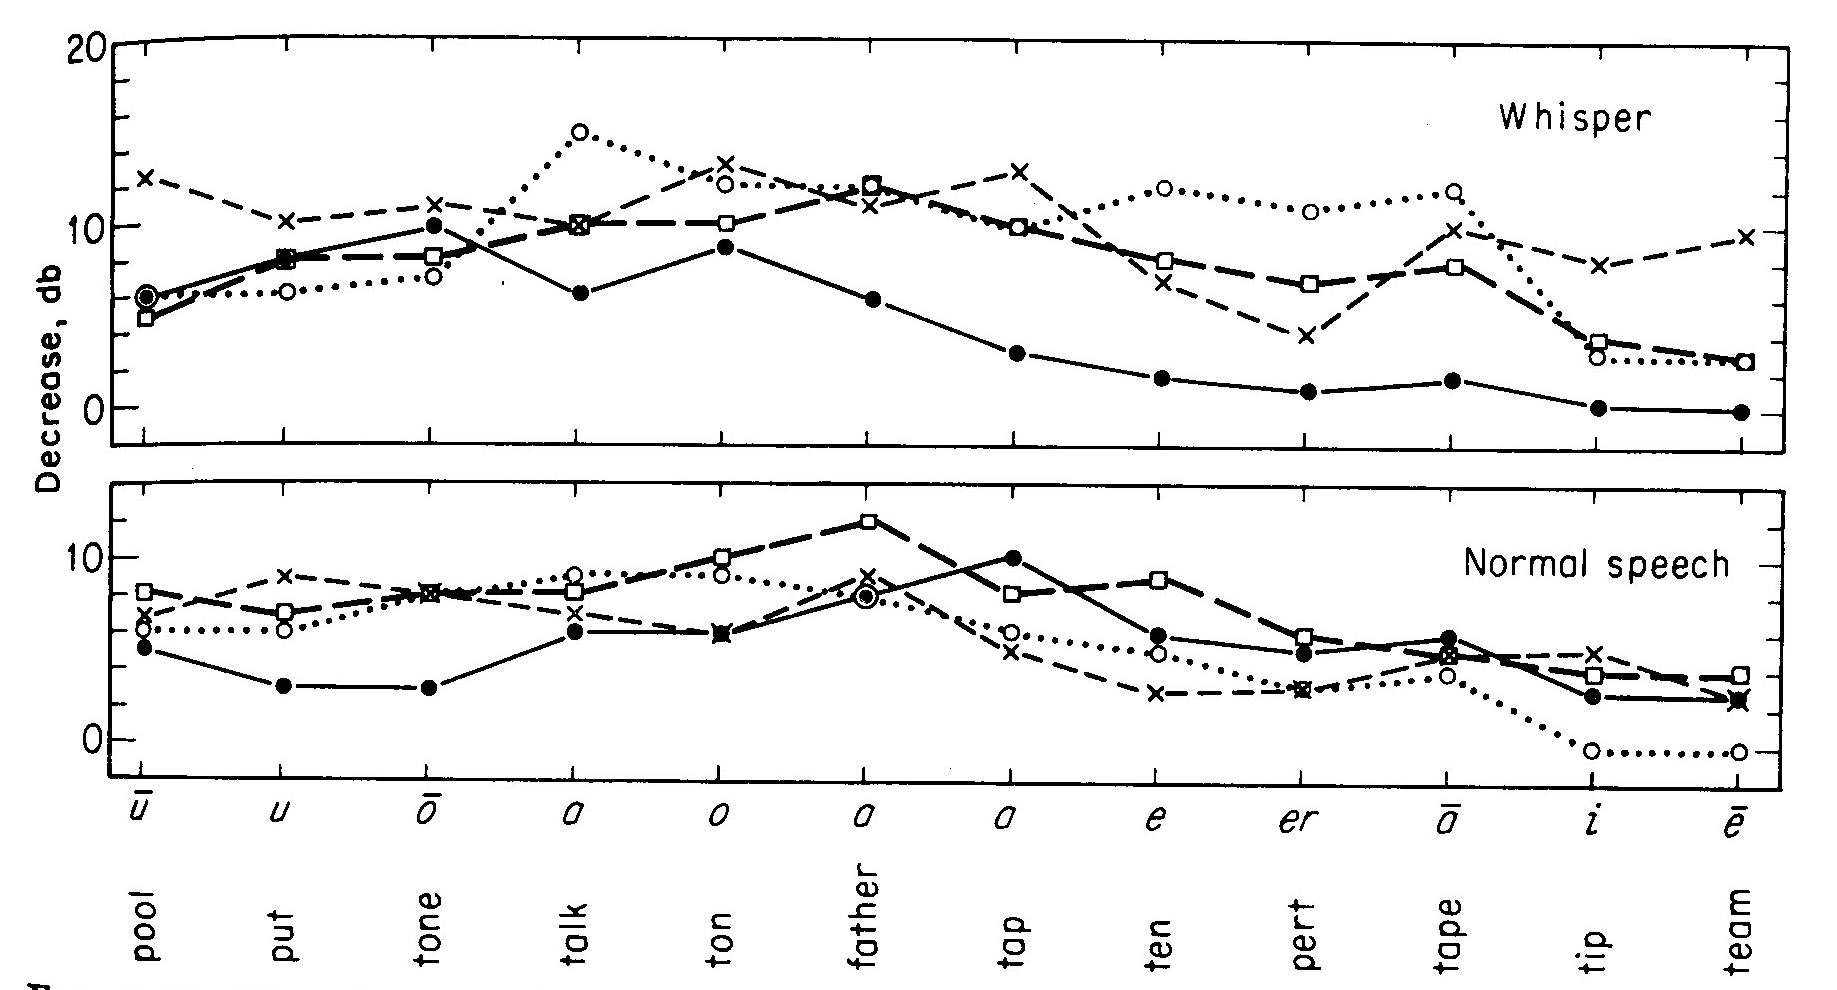
\includegraphics[width=0.5\textwidth]{figure/bekesy60-3.png}
%DIF >  \caption{Demonstrated the different effect on amplitude that closing the ear canal has on the different vowels of English.  Taken from \cite{bekesy:60}.}
%DIF >  \label{bekesyPhoneDiff}
%DIF >  \end{wrapfigure}
\DIFaddend 

%BC+EC+OE% Discussion of the Occlusion Effect
\subsection{The Occlusion Effect on Bone-Conducted Speech}\label{sec:OEBCspeech}



Returning to the notion of tubes, if the ear were to be occluded at its one open end, the ear canal would shift from an open-closed tube to a closed-closed tube, and the frequency response would be altered accordingly.  This phenomenon, first noted by \cite{wheatstone:79}, is termed the occlusion effect (OE).  The occlusion effect (OE) is the change in sound pressure level (SPL) resulting from body-conducted vibrations emanating into, and reverberating within, a \textit{closed} ear canal.  Objectively, inside the ear canal, the sound pressure level at lower frequencies is increased when the ear canal is occluded.  This has been studied extensively (cf. \cite{wheatstone:79,kelly:37,littler:52,tonndorf:66}, among many others).  %Generally, the occlusion effect (OE) results in a great increase in the amplitude of frequencies below 1-2kHz, acting as a low-frequency gain\footnote{This ``gain'' is a result of the transfer of energy from the higher frequencies} and that the amplitude of higher frequencies is dampened (as previously mentioned in the observation in studies of cats (\cite{tonndorf:72}).

\DIFdelbegin \DIFdel{Of }\DIFdelend \DIFaddbegin \DIFadd{This present section focuses on describing the occlusion effect, and what it means for bone conducted speech. Additionally, some factors that could potentially alter the effect of occlusion of the ear canal are mentioned, such as the depth of the occluding device inside the ear canal, the Lombard effect on speaker style, and changes to the size of the ear canal during jaw movement.
}


\DIFadd{Early on, the }\DIFaddend particular focus was \DIFaddbegin \DIFadd{to understand }\DIFaddend the mechanism behind this shift in amplitude to the lower frequencies. \cite{huizing:60} proposed that this `restructuring' of the frequency spectrum was due solely to the change in resonance characteristics of the ear canal when it is occluded.  This proposal is supported \DIFaddbegin \DIFadd{by }\DIFaddend the known physical phenomenon that the occlusion (or lack thereof) of ends of a uniform tube change the resonance properties of the tube. The resonance frequencies of an open-closed tube are proportional to 4x the length of the tube and a closed-closed tube produces resonant frequencies which are proportional to 2x the length of the tube.  Using the known characteristics of tube resonance to describe an occluded ear can partially account for what is observed\DIFdelbegin \DIFdel{; }\DIFdelend \DIFaddbegin \DIFadd{, but }\DIFaddend it largely describes what happens in the upper frequencies (generally above 2 kHz, \cite{stenfelt:03}).  

\cite{tonndorf:66}, through many studies utilizing domestic cats,  discovered the mechanism behind the apparent low-frequency gain.  When the ear canal is open, due to ``the mass-effect of the air column in the ear canal together with the compliance \DIFdelbegin \DIFdel{with the }\DIFdelend \DIFaddbegin \DIFadd{of }\DIFaddend air in the \DIFaddbegin \DIFadd{ear }\DIFaddend canal'' it acts as a high-pass filter, dampening the lower frequencies (\cite{stenfelt:03}, 910).  When the canal is occluded, this high-pass filter is gone, and the formerly filtered low-frequency energy \DIFdelbegin \DIFdel{is present within the canal}\DIFdelend \DIFaddbegin \DIFadd{reappears.  In this sense, it is not the case that the occlusion of the ear canal increases the amplitude of lower frequencies, but it prevents them from being filtered out}\DIFaddend .

%\cite{hansen:97b} and \cite{stenfelt:07} are primarily interested in modelling an occluded EAC, and this study requires the model to be a closed-closed tube - that of an \textit{occluded} ear. The models proposed by \cite{hansen:97b} and \cite{stenfelt:07} take many parameters, yet most can be considered to be either \textbf{too difficult to calculate frequently (- what does this mean? give an example)}, or relatively constant (e.g. the impedance of the middle ear, the speed of sound, etc.).  Both models, however, take the parameters for the length of the EAC, the average cross sectional area or diameter, and the volume of the EAC, which, are highly variable.

 
As with bone conduction in general, most of the research of the occlusion effect (OE) has been conducted using controlled mechanical vibrations.  Using a mechanical stimulus, \cite{bekesy:60} reported that when the ear canal is closed, the increase in amplitude within the canal can be observed up to 2 kHz, and above 2 kHz, the increase in loudness `vanishes' quite suddenly\DIFdelbegin \DIFdel{(cf. Fig. \ref{fig:bekesyOEresponse}). }%DIFDELCMD < 

%DIFDELCMD < %%%
\DIFdel{However, there is a variance in the OE - if using a mechanically-created vibration - depending on the location of stimulation.  This difference is most present in the lower frequencies (\mbox{%DIFAUXCMD
\cite{dean:00}
}%DIFAUXCMD
), where the relative amplitude increase of body-conducted sound versus air-conducted sound appears to be the greatest, but this difference tends to wash out when slightly higher frequencies are reached}\footnote{\DIFdel{\mbox{%DIFAUXCMD
\cite{dean:00}
}%DIFAUXCMD
found that the greatest relative amplitude increase occurs near 250 Hz, but the gain disappears when 1000 Hz is reached.}}%DIFAUXCMD
\addtocounter{footnote}{-1}%DIFAUXCMD
\DIFdelend . %DIF >  (cf. Fig. \ref{fig:bekesyOEresponse}).
\DIFaddbegin 

\DIFaddend There are also differences based on the location of \textit{occlusion} within the ear canal, ie. how deep a plug is placed in the ear canal.  This affects the resonant frequencies that play a part in the shape of the higher frequencies, due to the different depths of plug insertion resulting in `tubes' of different lengths.  Another effect of plug depth is that, the deeper a plug is inserted into the ear canal, the less surface area there is in the canal for acoustic vibrations to enter.  

\cite{dean:00}'s results indicate that the effect of plug depth on the amplitude of a signal does not disappear as frequency increases. The difference in relative amplitude between the different insertion depths is greatest at lower frequencies, with supra-aural earmuffs resulting in the greatest amplitude increase, and the deep inserted ear-plugs with the lowest.  However, at 1 kHz, the shallow-inserted ear-plug has a greater relative amplitude gain than the supra-aural earmuff.  \cite{dean:00} does not mention the explicit depth used for each condition. 


\cite{stenfelt:07} developed a model of an occluded ear using measurements generated from stimulating the skull separately at both the frontal bone and the mastoid process.
%
\DIFdelbegin %DIFDELCMD < \begin{wrapfigure}{r!}{0.5\textwidth}
%DIFDELCMD < 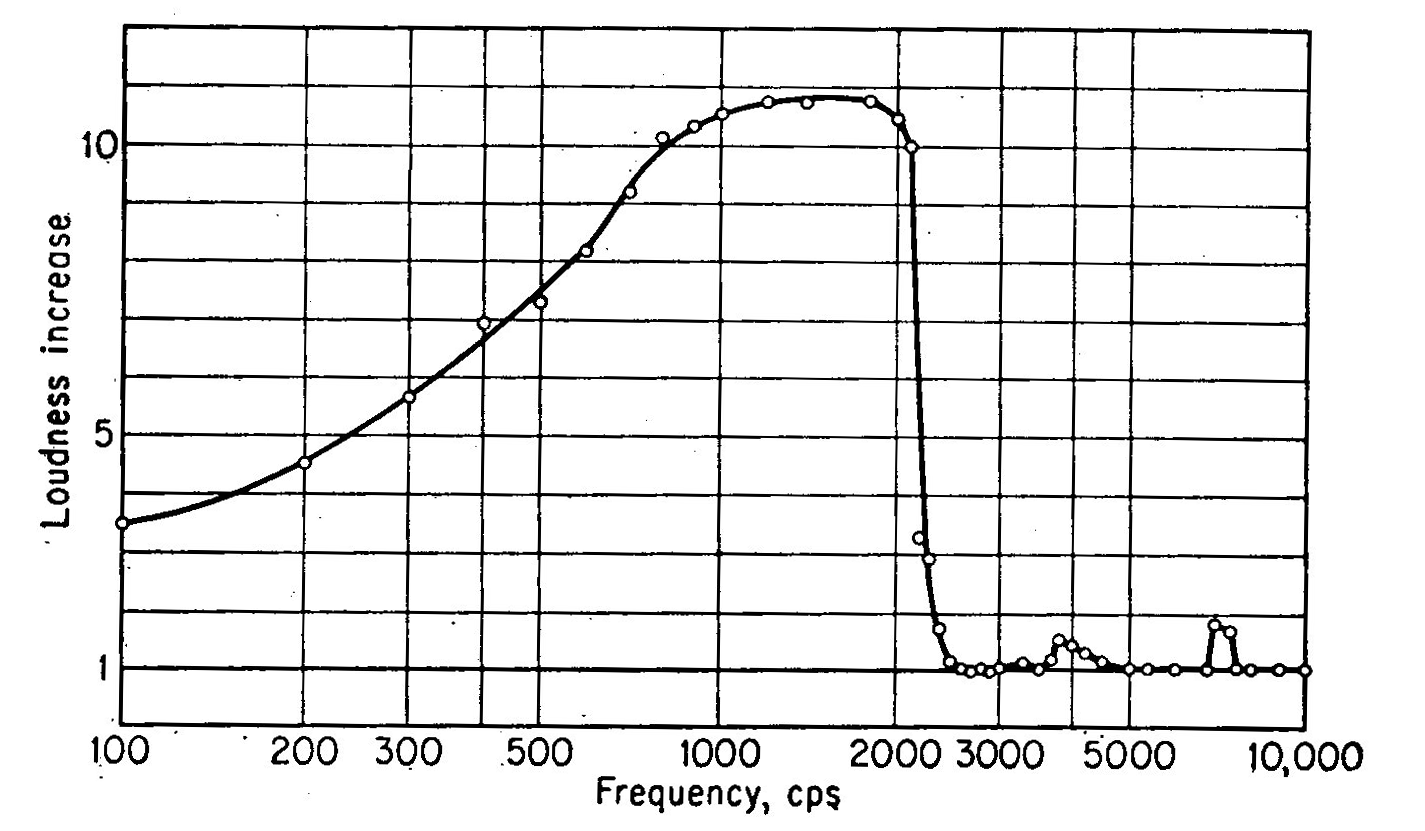
\includegraphics[width=0.5\textwidth]{figure/bekesy60-1.png}
%DIFDELCMD < %%%
%DIFDELCMD < \caption{%
{%DIFAUXCMD
\DIFdel{The frequency response inside the ear canal when taking a mechanical vibration as stimulus to a participant's forehead.  Taken from \mbox{%DIFAUXCMD
\cite{bekesy:60}
}%DIFAUXCMD
.}}
%DIFAUXCMD
%DIFDELCMD < \label{fig:bekesyOEresponse}
%DIFDELCMD < \end{wrapfigure}
%DIFDELCMD < %%%
\DIFdelend %DIF >  \begin{wrapfigure}{r!}{0.5\textwidth}
%DIF >  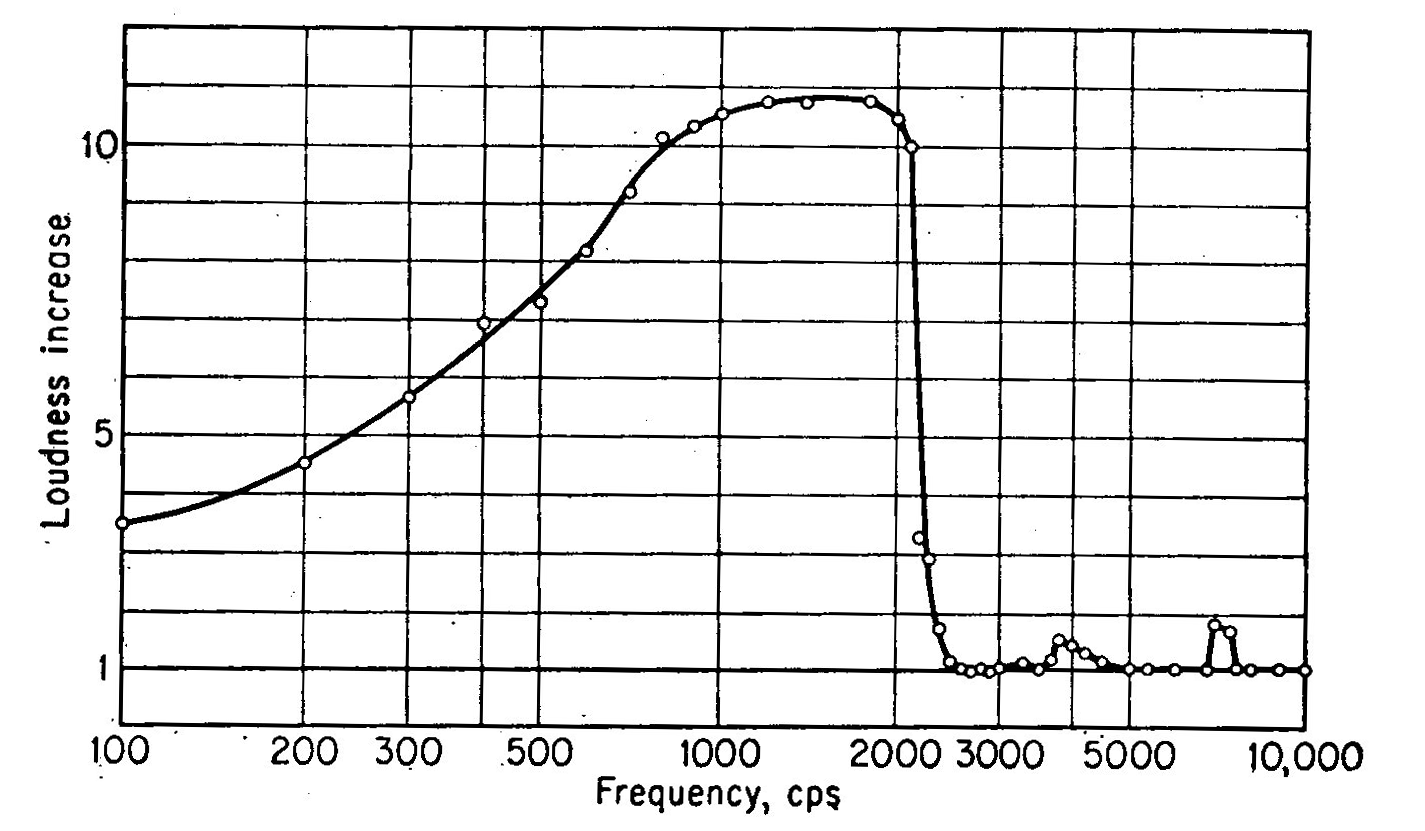
\includegraphics[width=0.5\textwidth]{figure/bekesy60-1.png}
%DIF >  \caption{The frequency response inside the ear canal when taking a mechanical vibration as stimulus to a participant's forehead.  Taken from \cite{bekesy:60}.}
%DIF >  \label{fig:bekesyOEresponse}
%DIF >  \end{wrapfigure}
%
\DIFdelbegin \DIFdel{Each site yielded a slightly different frequency response for the occlusion effect.  Stimulation at the mastoid generally resulted in a greater increase in very low frequencies below 1 kHz.  They also }\DIFdelend \DIFaddbegin \DIFadd{They }\DIFaddend noted that the OE was greatest when using an ear-plug near the opening of the ear canal, as opposed to supra-aural `earmuffs' or a deep-insertion ear-plug, though an OE was noticeable in each condition; this is in direct contrast with \cite{dean:00}\DIFaddbegin \DIFadd{, who found the greatest OE with the supra-aural earmuff}\DIFaddend .  \cite{dean:00} do not mention the size of earmuff used, but \cite{stenfelt:07} report the use of a \DIFdelbegin \DIFdel{large and small }\DIFdelend \DIFaddbegin \DIFadd{`large' and `small' }\DIFaddend earmuff, with the latter providing a greater OE than the former\DIFdelbegin \DIFdel{, though both }\DIFdelend \DIFaddbegin \DIFadd{; both are }\DIFaddend still below that of the shallow-insertion ear-plugs.

With shallow insertion, \cite{stenfelt:07}'s model estimates a gain in amplitude of frequencies below 2 kHz, and dampening of those above; all insertion depths, according to their model, will at minimum, slightly dampen frequencies above 2 kHz.  As the plug is inserted deeper, the damping occurs on lower and lower frequencies. These results contrast slightly with \cite{bekesy:60}'s\DIFdelbegin \DIFdel{in Fig. \ref{fig:bekesyOEresponse} }\DIFdelend %DIF >  in Fig. \ref{fig:bekesyOEresponse} 
in that they predict higher, very low frequencies, as opposed \DIFdelbegin \DIFdel{with }\DIFdelend \DIFaddbegin \DIFadd{to }\DIFaddend \cite{bekesy:60}'s\DIFdelbegin \DIFdel{bell-shaped }\DIFdelend %DIF >  bell-shaped 
resonance around 1-2kHz.

\DIFaddbegin \DIFadd{However, there is a variance in the OE - if using a mechanically-created vibration - depending on the location of stimulation.  This difference is most present in the lower frequencies (\mbox{%DIFAUXCMD
\cite{dean:00}
}%DIFAUXCMD
), where the relative amplitude increase of body-conducted sound versus air-conducted sound appears to be the greatest, but this difference tends to wash out when slightly higher frequencies are reached}\footnote{\DIFadd{\mbox{%DIFAUXCMD
\cite{dean:00}
}%DIFAUXCMD
found that the greatest relative amplitude increase occurs near 250 Hz, but the gain disappears when 1000 Hz is reached.}}\DIFadd{.  Each site in \mbox{%DIFAUXCMD
\cite{stenfelt:07}
}%DIFAUXCMD
's study yielded a slightly different frequency response for the occlusion effect.  Stimulation at the mastoid generally resulted in a greater increase in very low frequencies below 1 kHz.  This is one limitation of using a mechanical stimulus - it cannot be assumed to accurately model the occlusion effect of speech, since the observed effect differs depending on the location of the mechanical sitmulus.
}


\DIFaddend In contrast to the mechanical source studies above, \cite{hansen:97b} tested the OE using one's own voice as the input source.  \DIFdelbegin \DIFdel{\mbox{%DIFAUXCMD
\cite{hansen:97b}
}%DIFAUXCMD
presents a graph comparing three spectra calculated from continuous speech from three separate publications (From \mbox{%DIFAUXCMD
\cite{wimmer:86}
}%DIFAUXCMD
, \mbox{%DIFAUXCMD
\cite{thorup:96}
}%DIFAUXCMD
, and \mbox{%DIFAUXCMD
\cite{may:92}
}%DIFAUXCMD
, Fig. \ref{fig:hansenAverageOEa}).  
%DIF < 
}%DIFDELCMD < \begin{wrapfigure}{r}{0.5\textwidth}
%DIFDELCMD < \begin{subfigure}{0.45\textwidth}
%DIFDELCMD <   \centering
%DIFDELCMD <   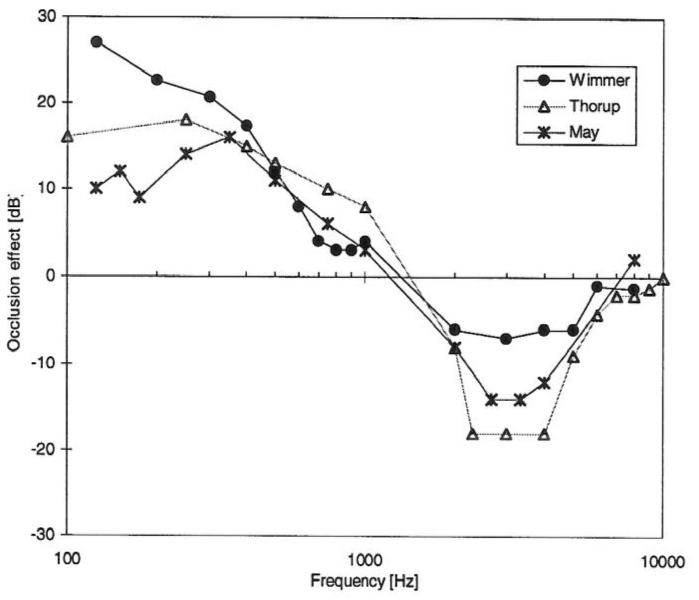
\includegraphics[width=0.8\textwidth]{figure/hansenAverageOE.png}
%DIFDELCMD <   %%%
%DIFDELCMD < \caption{%
{%DIFAUXCMD
}
  %DIFAUXCMD
%DIFDELCMD < \label{fig:hansenAverageOEa}
%DIFDELCMD < \end{subfigure}%%%
\DIFdelend %DIF > \cite{hansen:97b} presents a graph comparing three spectra calculated from continuous speech from three separate publications (From \cite{wimmer:86}, \cite{thorup:96}, and \cite{may:92}, Fig. \ref{fig:hansenAverageOEa}).  
%
\DIFdelbegin %DIFDELCMD < \hfill
%DIFDELCMD < \begin{subfigure}{0.5\textwidth}
%DIFDELCMD <   \begin{subfigure}{0.8\textwidth}
%DIFDELCMD <     \centering
%DIFDELCMD <     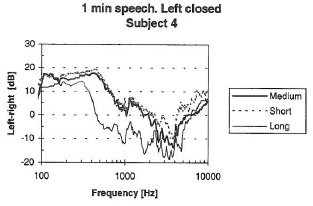
\includegraphics[width=1\textwidth]{figure/Hansen_OE-plot_a.png}
%DIFDELCMD <   \end{subfigure}
%DIFDELCMD <   \begin{subfigure}{0.8\textwidth}
%DIFDELCMD <     \centering
%DIFDELCMD <     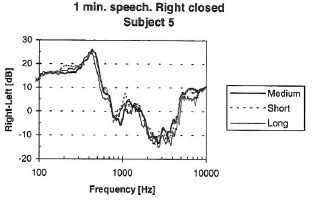
\includegraphics[width=1\textwidth]{figure/Hansen_OE-plot_b.png}
%DIFDELCMD <   \end{subfigure}
%DIFDELCMD <   %%%
%DIFDELCMD < \caption{%
{%DIFAUXCMD
}
  %DIFAUXCMD
%DIFDELCMD < \label{fig:hansenAverageOEb}
%DIFDELCMD < \end{subfigure}
%DIFDELCMD < %%%
%DIFDELCMD < \caption{%
{%DIFAUXCMD
\DIFdel{In (a), three separate measured OE spectra. In (b), OE of two subjects with ear molds extending into the canal at different lengths (\mbox{%DIFAUXCMD
\cite{hansen:97b}
}%DIFAUXCMD
).}}
%DIFAUXCMD
%DIFDELCMD < \label{fig:hansenAverageOE}
%DIFDELCMD < \end{wrapfigure}
%DIFDELCMD < %%%
\DIFdelend %DIF >  \begin{wrapfigure}{r}{0.5\textwidth}
%DIF >  \begin{subfigure}{0.45\textwidth}
%DIF >    \centering
%DIF >    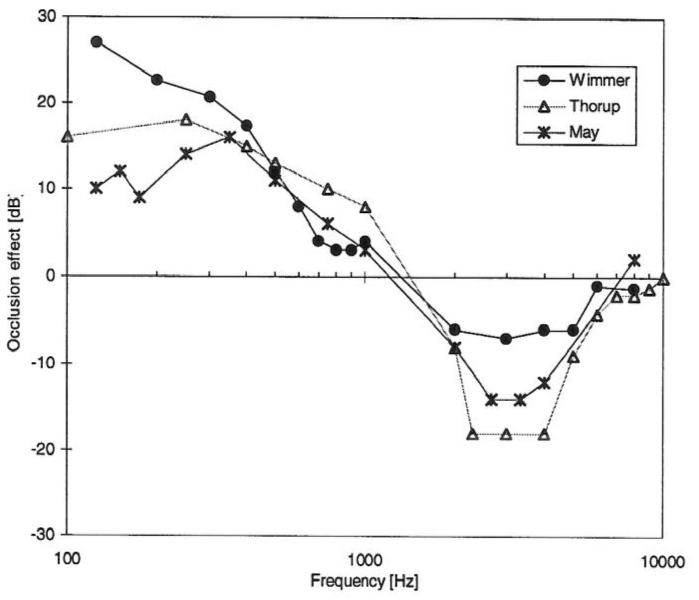
\includegraphics[width=0.8\textwidth]{figure/hansenAverageOE.png}
%DIF >    \caption{ }
%DIF >    \label{fig:hansenAverageOEa}
%DIF >  \end{subfigure}%
%DIF >  \hfill
%DIF >  \begin{subfigure}{0.5\textwidth}
%DIF >    \begin{subfigure}{0.8\textwidth}
%DIF >      \centering
%DIF >      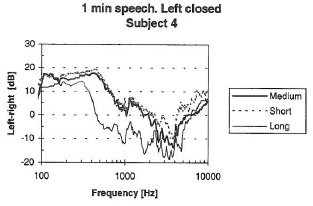
\includegraphics[width=1\textwidth]{figure/Hansen_OE-plot_a.png}
%DIF >    \end{subfigure}
%DIF >    \begin{subfigure}{0.8\textwidth}
%DIF >      \centering
%DIF >      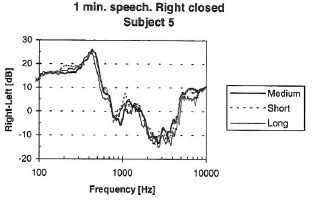
\includegraphics[width=1\textwidth]{figure/Hansen_OE-plot_b.png}
%DIF >    \end{subfigure}
%DIF >    \caption{ }
%DIF >    \label{fig:hansenAverageOEb}
%DIF >  \end{subfigure}
%DIF >  \caption{In (a), three separate measured OE spectra. In (b), OE of two subjects with ear molds extending into the canal at different lengths (\cite{hansen:97b}).}
%DIF >  \label{fig:hansenAverageOE}
%DIF >  \end{wrapfigure}
%
The study conducted its own tests \DIFdelbegin \DIFdel{(seen in Fig. \ref{fig:hansenAverageOEb}), }\DIFdelend %DIF > (seen in Fig. \ref{fig:hansenAverageOEb}), 
which, by and large, agree with \DIFdelbegin \DIFdel{the previous studies .  
These represent the `average' effect of occlusion on speech, and appear to resemble other (mechanical-source) estimations}\DIFdelend %DIF > the 
\DIFaddbegin \DIFadd{previous studies (\mbox{%DIFAUXCMD
\cite{wimmer:86}
}%DIFAUXCMD
, \mbox{%DIFAUXCMD
\cite{thorup:96}
}%DIFAUXCMD
, and \mbox{%DIFAUXCMD
\cite{may:92}
}%DIFAUXCMD
).  \mbox{%DIFAUXCMD
\cite{hansen:97b}
}%DIFAUXCMD
found, among much variation, that there was a substantial increase in amplitude below approximately 1 kHz, which dropped to around 0 dB amplitude increase relative to air-conducted speech, which held steady until approximately 2 kHz.  Between 2 kHz and approximately 5 kHz, there is a large dip, which above 5 kHz appears to result in another increase in amplitude}\DIFaddend .  \cite{hansen:97b} developed a model of the OE which largely agrees with these measurements\DIFaddbegin \DIFadd{, ie. very loud low frequencies, dampened mid-range frequencies, and another increase in frequencies above 5 kHz}\DIFaddend .

The increase in amplitude of the voice in the ear due to occlusion can also influence the manner in which speech is spoken.  This can be seen clearly by the OE's influence on the Lombard effect (\cite{lombard:11,lane:71}).  The Lombard effect is the tendency of humans to speak louder in noise due to noise interrupting the normal feedback loop of speech, ie. speakers do not hear themselves nearly as well in noise as they do normally, and so they speak louder (and clearer) to compensate.  However, recent research by \cite{brungart:12} demonstrated that the Lombard effect disappears when a participant is wearing ear-plugs in a noisy environment.  This is actually due to the presence of the OE, and the increase in amplitude of one's own voice by closing off the entrance to the ear canal.  Instead of an interruption in, or lack of, feedback, the occlusion provides the speaker with much louder feedback.  \cite{brungart:12} found that speakers wearing ear-plugs in a noisy environment actually speak \textit{quieter} than those without ear-plugs, \textit{regardless} of the actual noise-attenuation by the ear-plugs.  This indicates that it isn't necessarily the lack of noise that prompts speakers to \DIFdelbegin \DIFdel{use }\DIFdelend \DIFaddbegin \DIFadd{speak at }\DIFaddend a lower volume\DIFdelbegin \DIFdel{level, but }\DIFdelend \DIFaddbegin \DIFadd{, but rather }\DIFaddend the presence of occlusion and the consequent increase in amplitude of their own voice.

Yet despite an increase in overall amplitude \DIFaddbegin \DIFadd{of the voice}\DIFaddend , the OE does not alter all speech sounds equally.  The studies looking at the OE of human speech result in similar spectral resonances as those dealing with simple mechanical vibrations, except real-speech studies are able to capture the different OE for different kinds of complex sounds in a real speech environment, such as vowels.  



%% Allaying concerns of the effect of jaw movement on the occlusion effect.
\DIFdelbegin \DIFdel{While \mbox{%DIFAUXCMD
\cite{hansen:97b}
}%DIFAUXCMD
found }\DIFdelend \DIFaddbegin \DIFadd{\mbox{%DIFAUXCMD
\cite{hansen:97b}
}%DIFAUXCMD
found several }\DIFaddend phone-specific differences in the occlusion effect (OE)\DIFdelbegin \DIFdel{, it }\DIFdelend \DIFaddbegin \DIFadd{. It }\DIFaddend is ambiguous as to whether the differences are solely due to the differences in the transforms of phones as a result of body conduction (as seen \DIFaddbegin \DIFadd{above }\DIFaddend in \cite{reinfeldt:10}), or if there are sound-specific differences introduced within the ear canal or by the occlusion effect itself.  
Some have posited that variability could critically stem from the placement of the jaw bone during speech next to the external auditory meatus, and as that changes as the jaw moves up and down for `higher' or `lower' phones (eg. /i/ vs /a/). The placement of the jaw bone, as it moves changes the impedance characteristics of the vibration of the mandible against the temporal bone that houses the meatus (\cite{bekesy:60}).  \cite{allen:60} studied the OE on participants with a unilateral resection of the mandible (one side of the jaw has been removed), and found essentially no distinction between the OE in either ear (ie. with a mandibular joint adjacent to the cartilage of the ear canal or without).

Yet, \cite{hansen:97b}) found that a change in shape of the ear canal due to different jaw positions can create an acoustic `leak" between the ear canal wall and the occlusion device; the occlusion effect, obviously, behaves differently when there are different sized `leaks' resulting in different levels of partial occlusion. 
\cite{hansen:97b} diagrams cross sections of the ear canal with the jaw at different positions; between a closed jaw and 5mm of opening, there is relatively little difference between the shapes of the ear canal.  Since \cite{borghese:97} found that the jaw moves relatively little vertical distance during actual speech (max opening approx. 6 mm), it can be assumed that the ear canal changes shape negligibly during normal speech with a snug-fitting occlusion device. 

In summary, \DIFdelbegin \DIFdel{it is important to emphasize the key difference between measurements from an open ear canal and those from an occluded ear canal, which can largely be seen between Figs. \ref{BCrelACall} and \ref{fig:hansenAverageOEa}}\DIFdelend %DIF > it is important to emphasize the key difference between measurements from an open ear canal and those from an occluded ear canal, which can largely be seen between Figs. \ref{BCrelACall} and \ref{fig:hansenAverageOEa}.  
\DIFaddbegin \DIFadd{this section introduced the occlusion effect and its expected frequency response}\DIFaddend .  There is a \DIFdelbegin \DIFdel{massive increase}\DIFdelend \DIFaddbegin \DIFadd{large `increase' }\DIFaddend in the amplitude of the lower frequencies, which is not present from an open-closed ear canal, and a sizable drop in amplitude after 2kHz, which similarly does not seem to manifest itself when the ear canal is not occluded.  \DIFaddbegin \DIFadd{Another rise in amplitude can be seen above 5 kHz.  The jaw movement during speech is negligible, and is not expected to result in any noticeable effect on the OE.  The OE actually results in speakers talking quieter in noise with the ear occluded, because they have louder feedback (ie. the Lombard effect does not occur).  Finally, placement of the occlusion device does matter, as deeper placed plugs result in even greater dampening of mid-range frequencies.
}\DIFaddend 


%CONCLUSION
\subsection{Summary}

The aforementioned studies on \DIFdelbegin \DIFdel{body conduction}\DIFdelend \DIFaddbegin \DIFadd{bone conduction, ear canal resonance, }\DIFaddend and the occlusion effect, as would be expected, have indicated a large amount of inter-person and inter-phoneme variability \DIFdelbegin \DIFdel{, }\DIFdelend and have shown the complexity involved in estimating the effect of body conduction and ear canal reverberance on speech entering the ear canal.  However, the transfer function from the vocal tract to the ear canal does have some standard characteristics, namely, the body and (occluded) ear canal work in conjunction as a low-pass filter on speech, removing many of the higher frequencies which are within range of containing critical components for speech intelligibility.  \DIFaddbegin \DIFadd{The occlusion of the ear canal allows these lower frequencies to be fully realized.
}\DIFaddend 

%CONCLUSION to expt 1 lit review

%There is a possibility that the ear signal might be so low-pass filtered as to dampen the upper frequencies beyond retrieval and to the point that accurate recognition is unlikely.  In this case, there are still several possibilities, one of which will be outlined below.  

%While critical speech information may be lost, there is still critical speech information that will be present in the signal, namely the pitch.  The ear signal could be used to ``clean" a simultaneously recorded signal obtained from the mouth (which includes any ambient noise).  Since the occlusion effect acts as a gain in the low frequencies, the harmonic information of the voice signal can be reliably obtained from the ear signal.  Using this harmonic information, a comb filter (cf. \cite{nehorai:86}) could be developed and applied to the noisy mouth signal (cf. \cite{king:08}, \cite{cai:09}, \cite{jin:10}).  The comb filter acts as a series of narrow bandpass filters at equal (harmonic) intervals; when applied to speech, this can filter out the noise located in-between the harmonics.  

%There are a number of drawbacks with this method, however.  One is that this method primarily is used to recover voiced (harmonic) sounds, and fricatives or other voiceless sounds may not be able to be `cleaned'.  Another is that while speech is generally harmonic-like, it is not a perfectly harmonic signal, and there is a possibility that some of the higher harmonics might be accidentally filtered out.  This is particularly concerning as the higher frequencies are what is missing from the ear-recorded signal in the first place.


The methods described in this section, namely the models and transfer functions used by \cite{hansen:97b}, \cite{stenfelt:07}, and \cite{reinfeldt:10}, predict a general \DIFdelbegin \DIFdel{resonance within a closed ear canal that cause relatively higher amplitude }\DIFdelend \DIFaddbegin \DIFadd{relative emphasis }\DIFaddend in the lower frequencies (below 2 kHz) \DIFaddbegin \DIFadd{when the ear canal is occluded}\DIFaddend , and a drop in frequencies above that range (with a \DIFdelbegin \DIFdel{few exceptions}\DIFdelend \DIFaddbegin \DIFadd{rise above 5 kHz}\DIFaddend ).  With this knowledge, it appears that it may be possible for recoverable speech information to be recorded from inside the ear canal.  While the skull will prevent much ambient noise from reaching a microphone placed in the ear canal, an occlusion device would need to be placed at the opening of the canal to aid in dampening the noise.  This occlusion results in the distortion described above.

This distortion is hypothesized to be, by and large, predictable (\DIFdelbegin \DIFdel{\mbox{%DIFAUXCMD
\cite{reinfeldt:10}
}%DIFAUXCMD
}\DIFdelend \DIFaddbegin \DIFadd{\mbox{%DIFAUXCMD
\cite{hansen:97b,reinfeldt:10}
}%DIFAUXCMD
}\DIFaddend ), unlike ambient noise from the environment which is generally highly variable in both amplitude and form (\cite{zhang:17}). This prediction is that the signal recorded from the ear canal is expected to be heavily low-pass filtered above approximately 2kHz.  Minor transformations, such as pre-emphasizing the higher frequencies, are hypothesized to recover some of the information that is lost, resulting in speech that will perform better than a noisy signal collected at the mouth in both ASR and human speech perception tasks.
Due to this, the technique of substituting potentially unanticipated, variable `environmental' noise with the anticipated `noise' of body conduction and the occlusion effect will allow for greater confidence that a usable signal could be recovered.    

Section \ref{expt1} below describes the specific methods used to collect speech data from the mouth and the ear canal, and the analysis of the collected speech in an attempt to recover an intelligible signal with the knowledge outlined in this section.  These recovered signals were used in human speech perception and ASR experiments in Chapter \ref{chapter3} and \ref{chapter4}, respectively.


\section{Experiment 1: Creating a dataset of ear-recorded speech}\label{expt1}

There are numerous constraints and requirements for the speech recordings necessary for this task, and it was essential to create an original dataset for this study.  This small corpus was used for creating stimuli ASR and human speech perception experiments.  Primarily, an original corpus needed to be created because there is no known dataset of speech in which the recording location is inside the ear canal; speech recorded from this location was the primary focus of these studies.  Secondly, in order to be comparable, the speech at the ear, and the speech at the mouth, needed to be recorded at the same time, in the same conditions.  This was mainly to determine, when comparing the results of ear-recorded and mouth-recorded speech, whether the ear or mouth-recorded speech performed better in the ASR and human speech perception tasks and to avoid potentially confounding variables that would occur if the two sets of speech were recorded separately. This is discussed further in Section \ref{chap2:methods:design} below.

\subsection{Design}
\label{chap2:methods:design}

The goal of this experiment was to create a dataset of recordings, both from the mouth, in noisy conditions, and from inside the ear in the same conditions.  These recordings were needed to test the following (previously mentioned) hypotheses: (a) whether recording speech from the ear, external noise would be completely or largely eliminated, while simultaneously recorded speech from the mouth had a noisy background, (b) whether the speech from the ear was more intelligible and recognizable by an ASR system than noisy speech, and (c) whether the speech from the ear is more intelligible and recognizable by humans than noisy speech. 

In alignment with the CHiME challenge\footnote{The CHiME challenge tasks researchers to improve upon or surpass the performance of a baseline automatic speech recognizer used on noisy speech data.} guidelines, this study uses different types of background noise at different noise levels.  The noises used include the four sounds (bus, caf\'{e}, pedestrian area, \& street) from the \cite{chime:16}, plus a `factory' noise track.  A short portion of the audio with relatively level amplitude was extracted from each sound file to be played in the background.  Relatively level amplitude was used to allow for a more accurate comparison of the different SNR levels. Furthermore, if a sound file varied in amplitude, it would confound the recognition tasks as to whether a certain word is difficult to recognize, or the noise level that occurred at that portion in the sentence was a hindrance to accurate recognition.\footnote{The exact portions of the sounds which were used are available online, along with the rest of the data at http://www.openslr.org/}

Many existing works in ASR and human speech recognition in noise use multiple SNR levels to demonstrate the effectiveness of the technique of noise removal (eg. \cite{braun:16}).  This is generally done by adding a noise signal to already recorded clean speech, giving the researcher acute control over the SNR.  Recording the noise while simultaneously recording the speech was necessary to demonstrate the ability of the ear canal recording location to remove ambient noise.  Due to this need, it was determined that noise would be played from a loudspeaker at pre-determined decibel levels.  

Since human speech is variable in loudness, and amplitude will likely vary between and within speakers, only three, well-spaced noise levels were chosen to allow speakers' various `loudnesses' to fall in the same, broad categories.  Conversational speech is generally around 70 dB, and so the noise levels chosen were 60 dB, 70 dB, and 80 dB.  These were the `averaged' dB levels obtained by averaging over the duration of the sound file.  This would result in approximate SNR conditions of +10 (60 dB), 0 (70 dB), and -10 (80 dB).  A signal with +10 dB SNR is in the range of SNRs where ASR and human listeners have a very high recognition accuracy (cf. \cite{braun:16,gilbert:13}).  A signal with 0 dB SNR occurs in a range in which ASR and human listeners are still able to make out most of a speech signal, but recognition begins to falter.  At -10 dB SNR, recognition performance very noticeably suffers.  As stated before, it was assumed that speakers will vary in how loud they speak, and so actual SNRs were expected to vary.

An amplitude of 80 dB was chosen as a max loudness, rather than a higher noise level to achieve a lower SNR, in order to leave a wide margin between it and any (albeit remote) possibility of hearing damage suffered by participants.  A `clean' (no noise) condition was also utilized for each sentence.  This creates 16 different conditions (5 noise types * 3 noise levels + 1 `clean' condition).  

\subsection{Stimuli}
Thirty sentences were chosen from 3 Harvard Sentence lists\footnote{The `Harvard Sentences' dataset is comprised of 72 lists, each 10 sentences long, where each list of 10 sentences is phonetically balanced, where the proportion of each phone in the list corresponds with it's occurrence in the English language (\cite{harvardSents}).}.  Sentences were chosen from the Harvard Sentence dataset due to being phonetically balanced (the distribution of phonemes in each list proportional to their occurrence in English), to their prolific use in speech science research, and specifically their history of serving as stimuli for many speech corpora (cf. \cite{kabal:02,hu:07}, the latter being a noisy speech corpus).  Lists 14, 28, and 57 were used, and chosen semi-randomly, eliminating lists with potentially unfamiliar or rare words.  Each sentence occurs in all 16 conditions (5 noise types * 3 noise levels + 1 `clean' condition), resulting in 480 total stimuli.

  
\subsection{Equipment}

The experiment took place in a large soundbooth.  To create the artificially noisy environment a Yamaha MS101 III loudspeaker was hooked to an HP ProBook 6470b laptop.  A sound pressure level meter (SPL meter; Larson Davis Model 831) with a PCB Piezotronics Model 377B20 condenser microphone (omnidirectional) was placed 1 meter from the loudspeaker and measured the sound pressure to verify each of the three noise levels for each of the 5 noise types. A Grason-Stadler GSI Typstar Middle Ear Analyzer was used to measure the ear canal volume and test for plug leaks.  Two Countryman B2D directional lavalier microphones with fixed XLR connections were used to record the mouth speech and the ear speech.  These were hooked up to a PreSonus Digital Audio Firebox preamplifier, which was connected via TRS cables to a Zoom H6 Handy Recorder. A pair of 3M Professional Peltor Earmuffs with an noise reduction rating (NRR)) of -30 dB SPL were worn by the participants during the experiment.


\subsection{Participants}
\DIFdelbegin \DIFdel{Twenty participants were used in }\DIFdelend \DIFaddbegin \DIFadd{Seventy-one participants were run for }\DIFaddend this study, \DIFaddbegin \DIFadd{but data from only twenty participants was used, }\DIFaddend ten female and ten male, all \DIFdelbegin \DIFdel{native }\DIFdelend \DIFaddbegin \DIFadd{fluent }\DIFaddend speakers of American English with normal hearing.

\subsection{Procedure}\label{chap2:methods:procedure}

The participants were initially asked a few preliminary demographic questions\footnote{eg. 2nd language (if any), etc. For a list of all information gathered, see Appendix \DIFdelbegin \DIFdel{A}\DIFdelend \ref{appendixA}.}. They were seated in front of the Middle Ear Analyzer.  An otoscope was used to ensure the right ear was mostly free of cerumen, to avoid blocking the microphone off from the rest of the canal and generally impacting the canal with cerumen.  The ear was fitted with an appropriate sized rubber clinical single-use ear tip, into which the Middle Ear Analyzer hose was already plugged.  An \DIFaddbegin \DIFadd{effort was made to ensure a relatively standard depth for the ear plug, as it plug depth has been shown to alter the OE (\mbox{%DIFAUXCMD
\cite{dean:00,stenfelt:07}
}%DIFAUXCMD
), but oftentimes this was not possible, and achieving a proper seal was given a higher priority.
}

\DIFadd{An }\DIFaddend immittance test was performed, which involves playing a tone, and slightly and briefly pressurizing the ear.  The Middle Ear Analyzer checked that the ear-plug solidly sealed off the ear canal in order to be able to build up pressure, and would alert the researcher to a leak if the plug were not securely in place.  This test gave an estimate of the volume in milliliters (mL) of the ear canal and of the middle ear, with precision to a tenth of a mL; additionally, a graph of middle ear function was given, which was checked for normalcy (cf. Appendix \DIFdelbegin \DIFdel{A}\DIFdelend \ref{appendixA}).  The Middle Ear Analyzer gave other measures which were not used in this study.

The distance from the end of the ear-plug to where it was enclosed by the ear canal was measured to determine how far the plug was inserted in the ear canal.
Since the length of the plug is known, this was done by placing a measuring rod against the cavity of the concha to measure how far the plug was sticking out of the ear, from which the insertion depth can be calculated. The decision to treat the cavity of the concha as the `end" of the ear canal was taken from \cite{stenfelt:07}, who made molds of ear canals, and treated the rapid increase in volume (where the cavity of the concha began) as the end to the ear canal.  This measure allowed for the calculation of the depth of insertion of the ear-plug.

\begin{wrapfigure}{R}{0.5\textwidth}
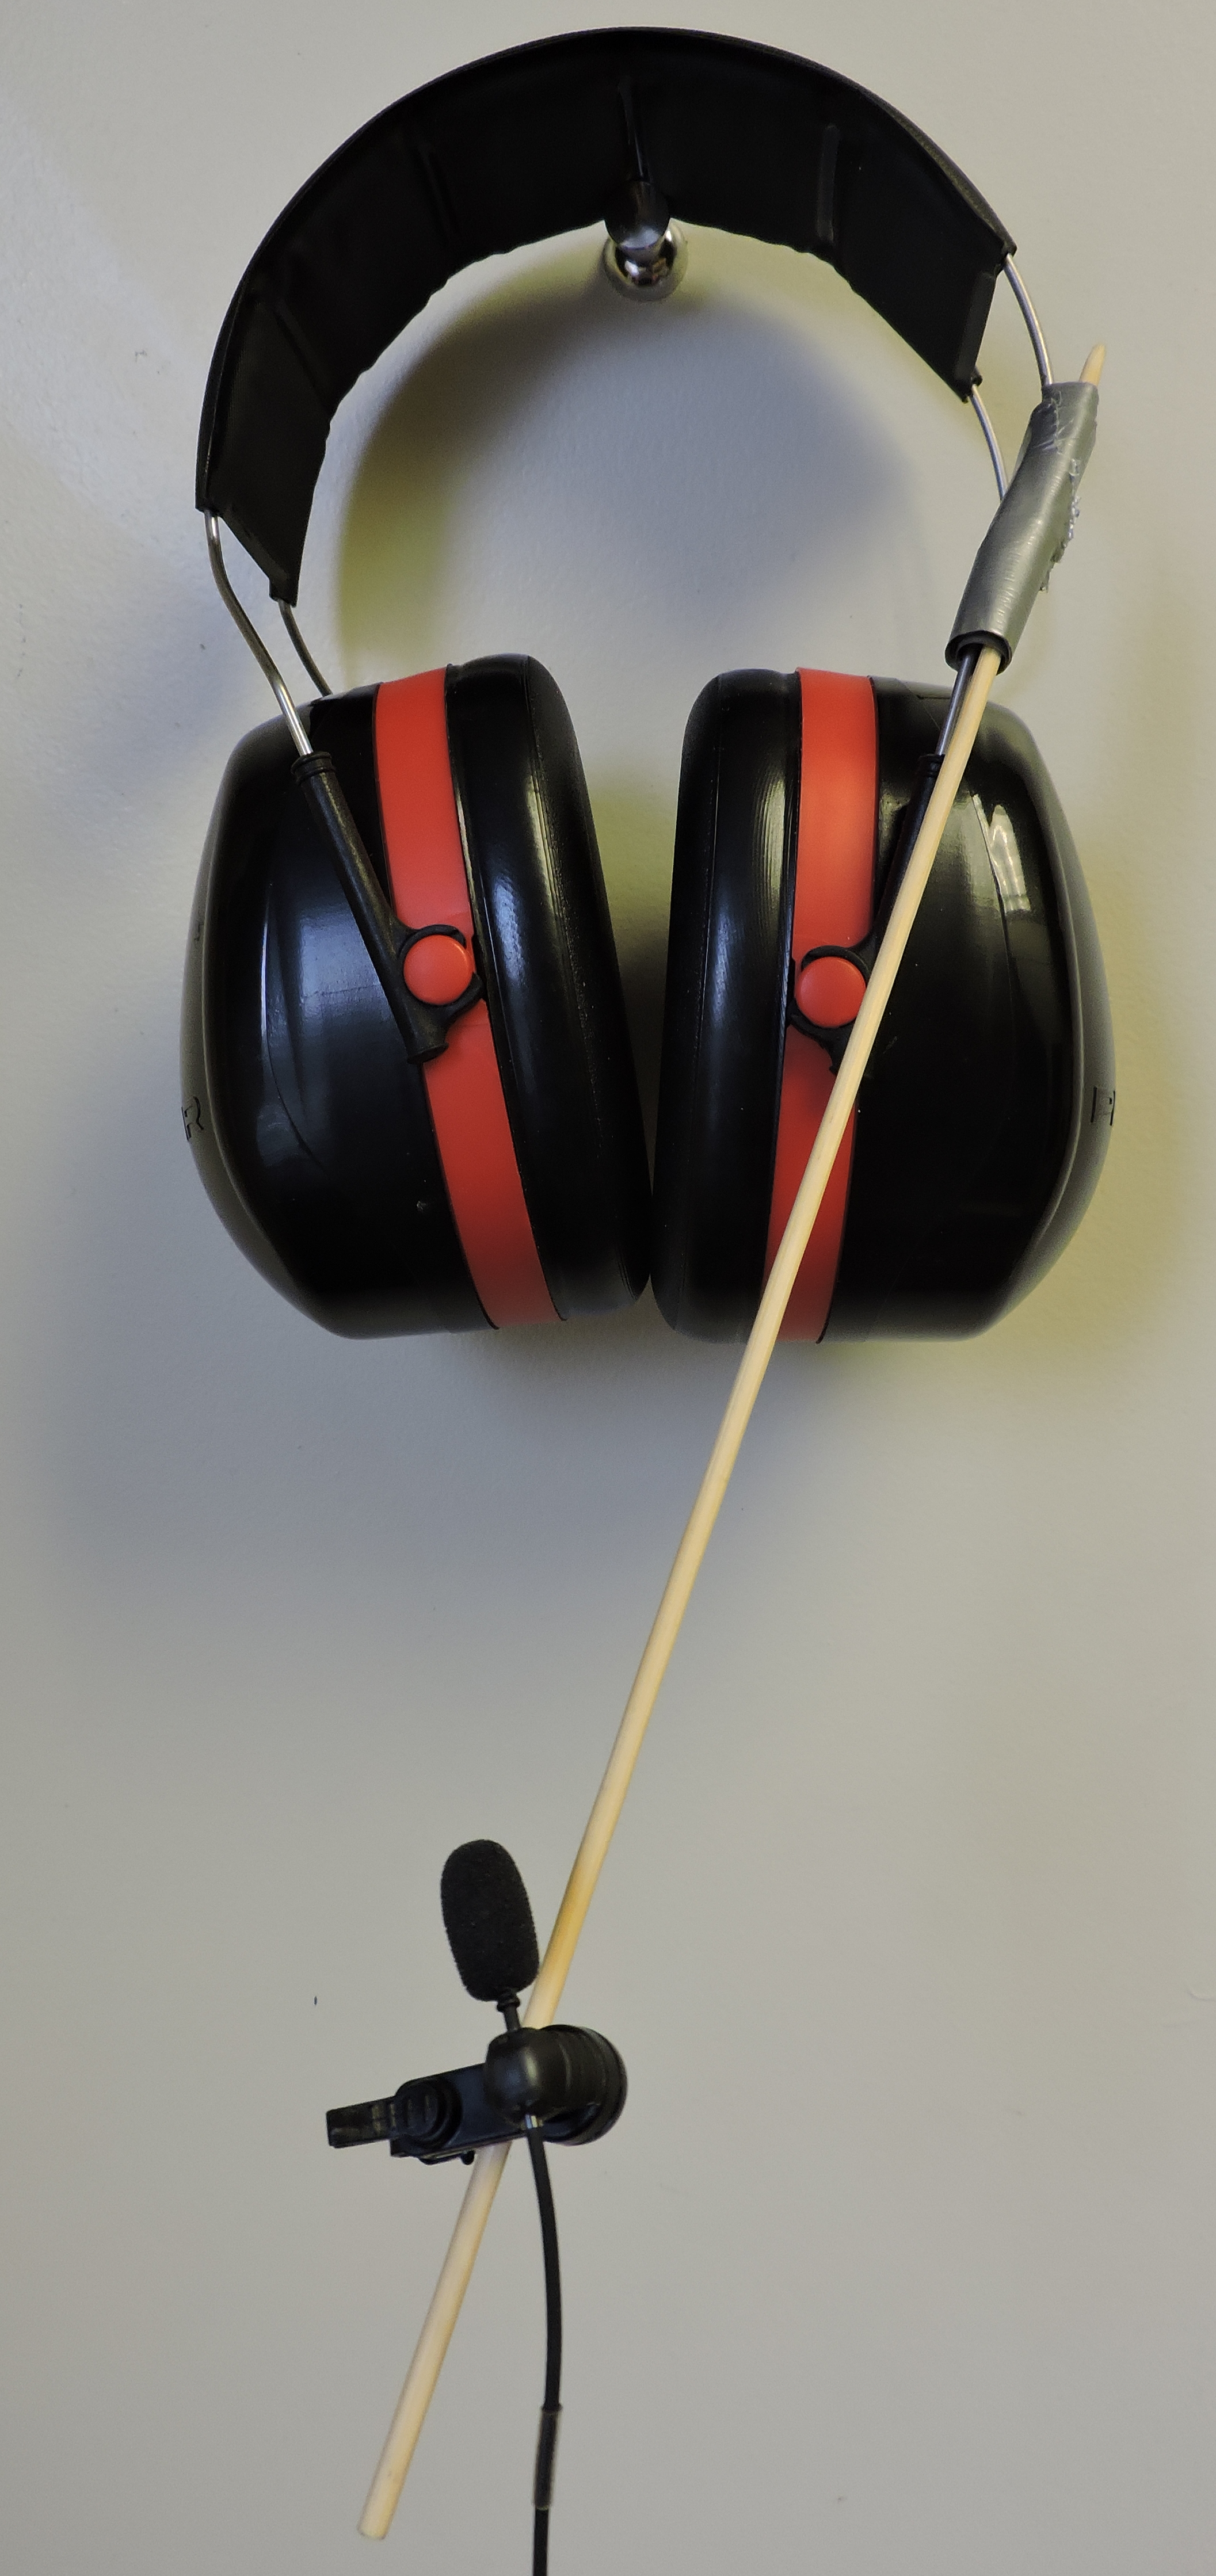
\includegraphics[width=0.5\textwidth]{figure/earmuffSetup.JPG}
\caption{The 3M 30 NRR earmuffs, a wooden rod attached with adhesive tape, and a Countryman B2D directional lavalier microphone directed toward the location of the mouth.}
\label{fig:micInsertPlug}
\end{wrapfigure}

\begin{wrapfigure}{L}{0.5\textwidth}
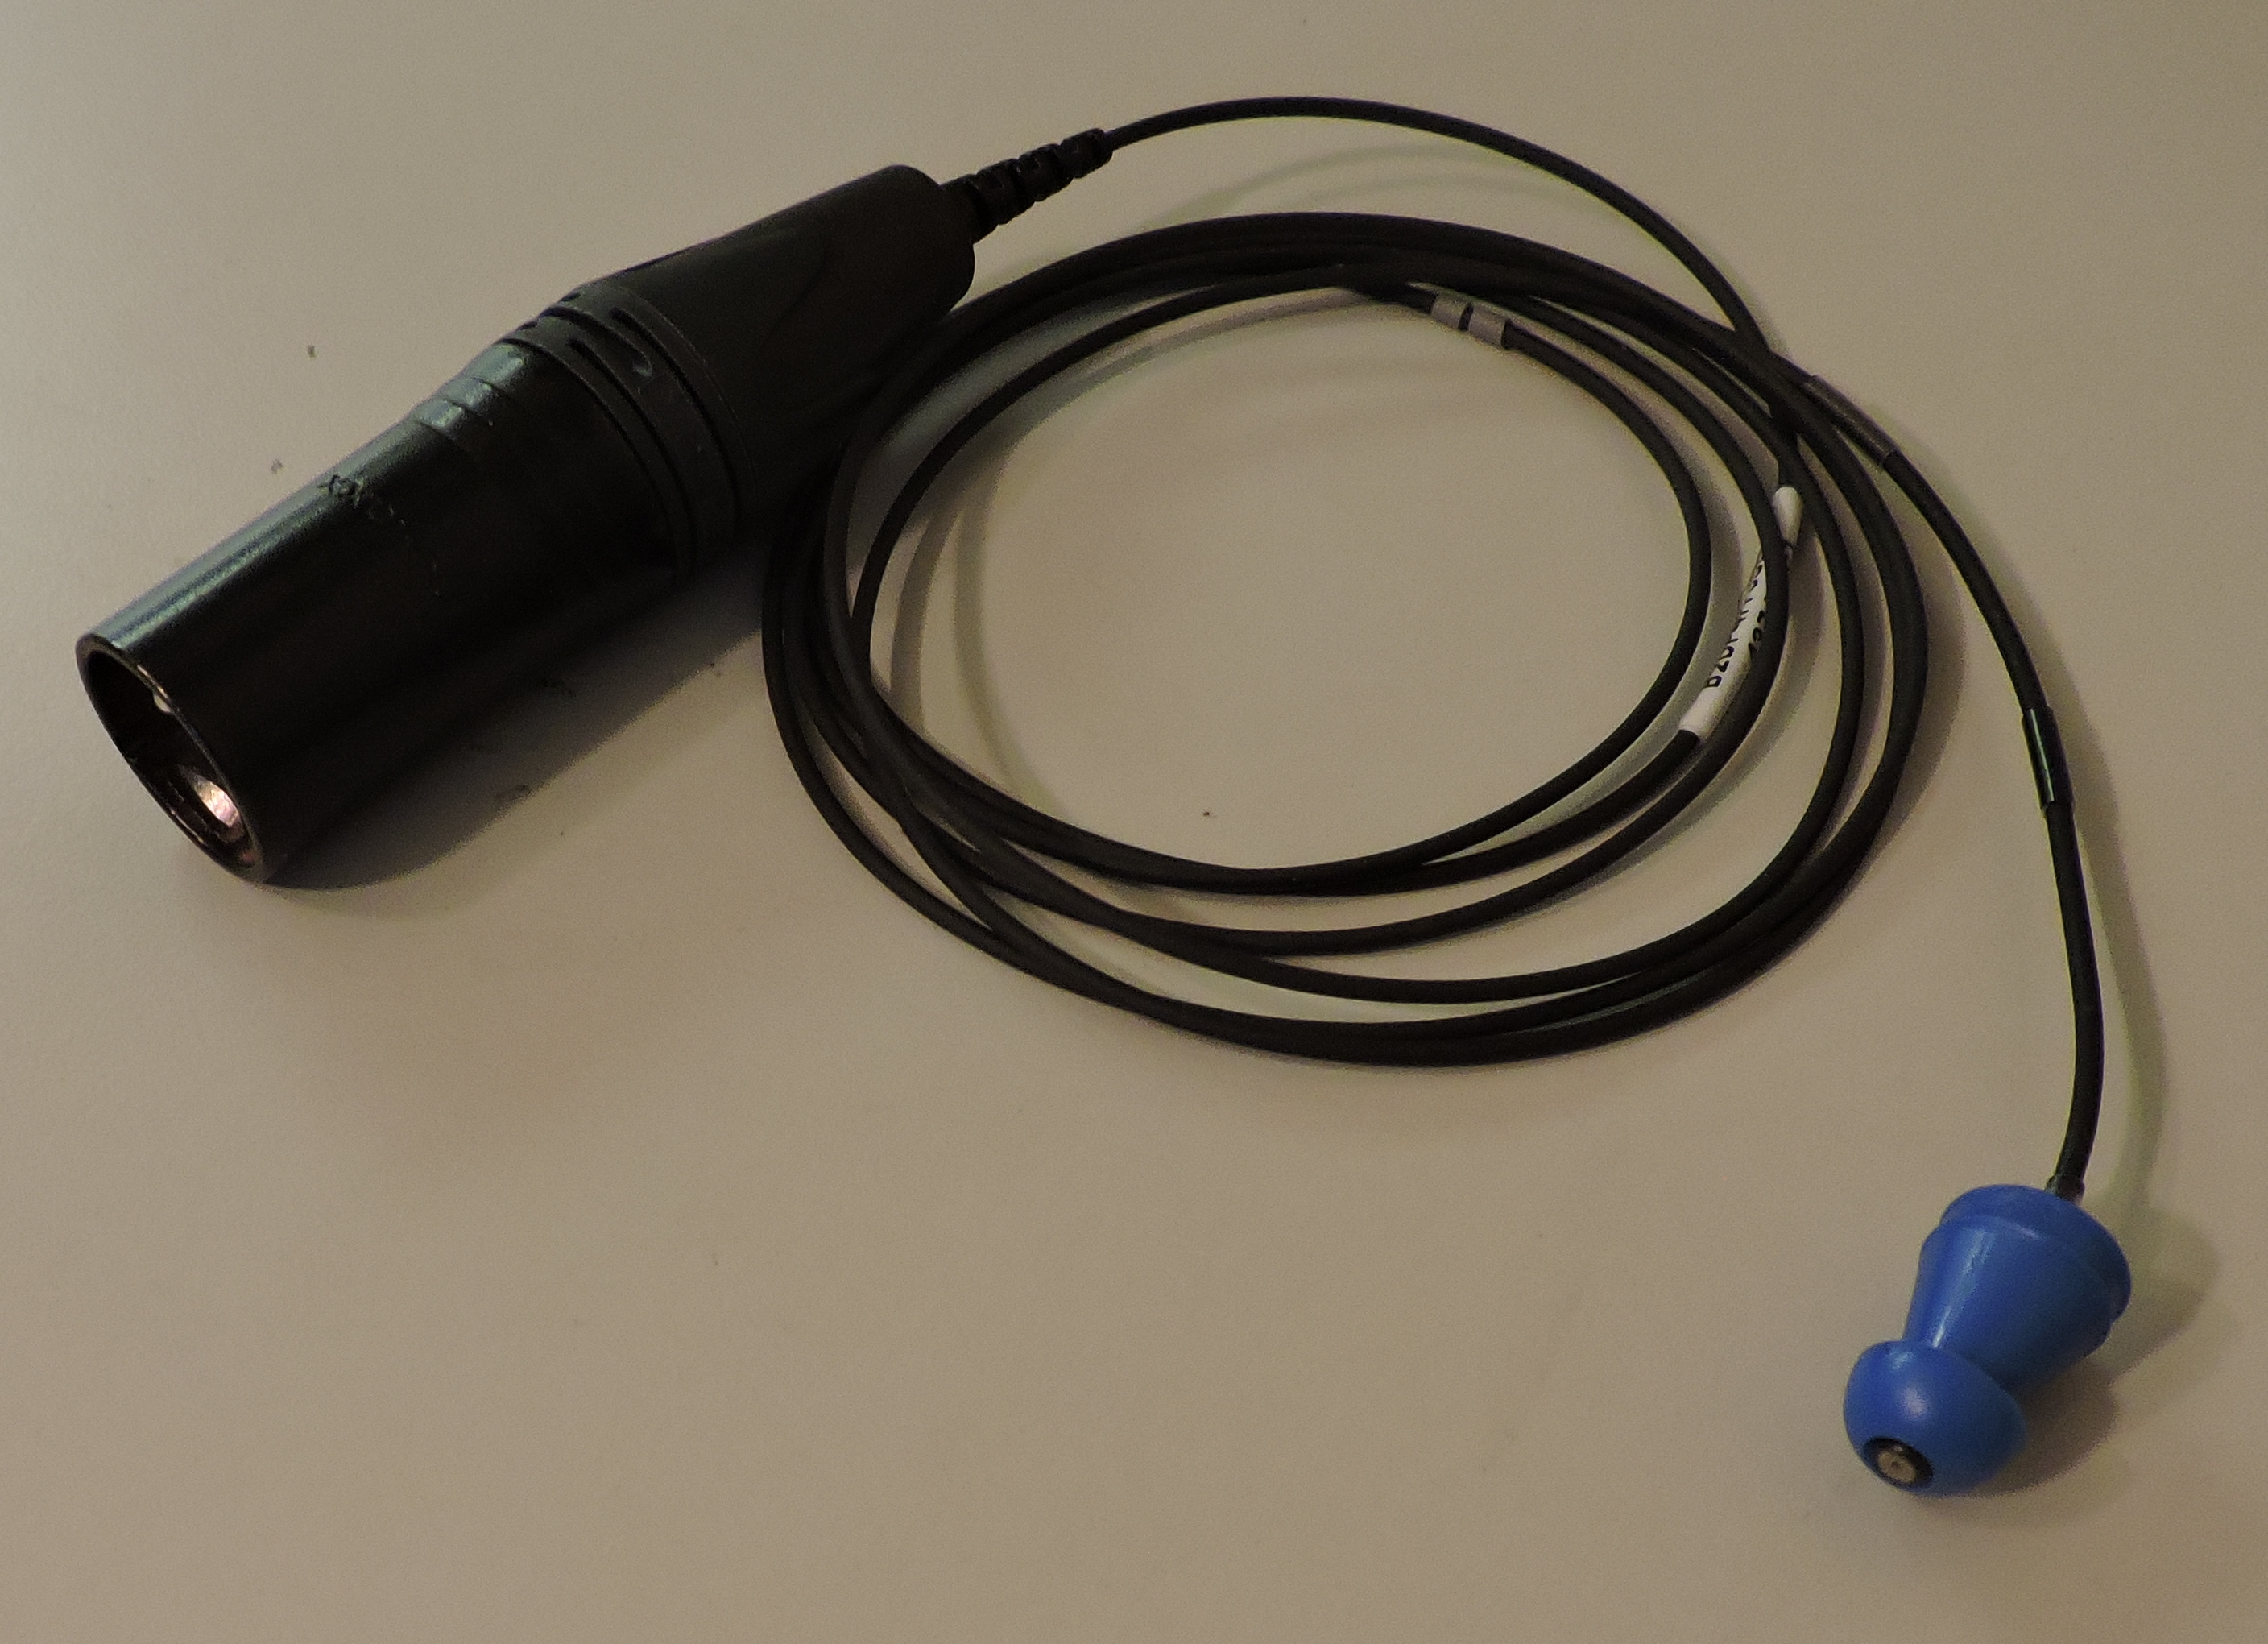
\includegraphics[width=0.5\textwidth]{figure/micInsertPlug.JPG}
\caption{The Countryman B2D directional lavalier microphone, with with the wind-break foam removed, and inserted into a blue ear-plug.}
\label{fig:earmuffSetup}
\end{wrapfigure}

The Middle Ear Analyzer hose was then removed from the ear-plug - which was carefully left in place to ensure a continuous seal.  The participants then moved to a seat located in front of a computer monitor (cf. Fig \ref{fig:overallSetUp} for set-up diagram).  The participants were then instructed as to the proceedings of the rest of the experiment. One of the two microphones was taken, the wind-break foam removed, and was snugly inserted into the ear-plug.  A mark on the microphone cable was used to ensure the end of the microphone was fully inserted to the end of the ear-plug (cf. Fig. \ref{fig:micInsertPlug}).  There were several instances where the microphone was inserted deeper than, or just shy of, the end of the ear-plug; the variance was within +/-2mm depth (cf. Appendix \DIFdelbegin \DIFdel{A}\DIFdelend \ref{appendixA}).  The earmuffs were placed over both ears.  Occasionally, participants had glasses, or thick hair, which may have slightly compromised the seal.  A note was taken of this. \DIFaddbegin \DIFadd{Necessarily, the cord for this microphone also ran from the microphone inside the ear-plug, out underneath the earmuff seal to the pre-amplifier.  This was assumed to not significantly effect the earmuff seal.
}\DIFaddend 

\begin{wrapfigure}{R}{0.5\textwidth}
\includegraphics[width=0.5\textwidth]{figure/overallSetUp.png}
\caption{A diagram of the basic equipment set up for the experiment.  The in-ear microphone is placed under the headphones in the right ear.}
\label{fig:overallSetUp}
\end{wrapfigure}

A wooden rod was attached to the earmuffs, which extended forward, beside the participants' face.  The second microphone was attached to this wooden rod via the lavalier clip at the level of the participants' mouth.  The microphone was directed toward their mouth (cf. Fig \ref{fig:earmuffSetup}).  
The placement of the microphone on the wooden rod was adjusted to be exactly 10cm away from the participants' infra-nasal depression.  At this point, the participants were asked to adjust the placement of their chair so that the microphone on the wooden rod would be approximately 1 meter from the loudspeaker. Due to the length of the experiment ($~$45min), no effort was made to discourage minor shifting in body position.  The loudspeaker was on another table to the right of the participants, perpendicular to the direction of the microphone facing the mouth (cf. Fig. \ref{fig:overallSetUp}).

Both microphones were connected directly to the preamplifier through a fixed (non-changeable) XLR connection.  Both channels were set to the same gain on the preamplifier.  Two TRS cables took each microphone signal from the preamplifier to the recorder.  Both channels were adjusted to appropriate (different) gain levels on the recorder itself to achieve a similar loudness for both signals and prevent clipping.  These adjustments were made once the participants were situated, but before beginning the recording.

Once recording, an in-house computer program was used to display the stimuli sentences on a second monitor and to play the background noises.  For each sentence, the participants saw the clean-condition (no noise) first.  The researcher was in the soundbooth with the participants listening through a pair of headphones connected to the preamplifier.  The participants were asked to repeat the sentence twice to develop a rhythm, at a normal, conversational loudness, with a normal, declarative intonation.  The researcher asked the participants to repeat the sentence again in this condition if the rhythm or intonation of the two sentences did not match, or if the participants stumbled over a word.  Each of the following 15 iterations of the sentence (one for each noise-type/noise-level combination) the participants were instructed to read the sentence aloud only once.  Out of the loudspeaker, placed 1 meter from the participants, each of the background noises were emitted to coincide with an iteration of the sentence.  If the rhythm of the spoken sentence varied noticeably, or if the participant stumbled over a word, the researcher again asked the participants to repeat the sentence for that condition.  The sentences were not randomized, ie. all 16 iterations of a sentence occurred consecutively\footnote{This was done to help the researcher ensure a similar intonation and rhythm for each iteration of the same sentence.}. \textit{Within} each sentence group (after the `clean' condition, which always occurred first), all the noise conditions were randomized. The researcher advanced each stimulus on the display for the participants.

To help the participants notice when a sentence had been advanced - as when wearing the noise reduction earmuffs, participants were often not aware when the noise condition changed - the number of the sentence condition was displayed underneath the stimulus (1-16).  This had the unintended consequence of occasionally producing a mild list-intonation, as participants were aware of the final repetition of a given sentence (ie. the number `16' appeared beneath the sentence). 

After the recording was finished, the participants were asked to complete a short, 4-question survey of their experiences during the experiment.\footnote{cf. Appendix \DIFdelbegin \DIFdel{A}\DIFdelend \ref{appendixA} for coded answers.}  These included:
\begin{enumerate}
  \item{Can you describe your experience with wearing the experimental set-up?}
  \item{Did you find the sound of your voice to be altered, annoying, or uncomfortable?}
  \item{Would you consider wearing such a device if in a noisy workplace or environment in order to communicate?}
  \item{Would you be more inclined to use such a device if earmuffs were not required?}
\end{enumerate}

Participants were instructed to give as much detail in their answers as desired, and to answer truthfully.  The answers to the first question that were provided by participants generally addressed the comfort of the experimental set-up (ie. the ear-mic and earmuffs).  The researcher used the more specific question -``Did you find the experimental set-up (ie. the ear-mic and earmuffs) uncomfortable?'' - to code the answers. The answers were coded using a Likert scale with a range of 1-5, where `5' is `yes - definitely' and `1' is `no - definitely not'.

\DIFdelbegin %DIFDELCMD < \section{Observations of Collected Speech}%%%
\DIFdelend \DIFaddbegin \DIFadd{Sentences were identified and extracted using Praat.  A number of subjects (more than 20) were recorded, but in an attempt to meet a number of conditions, only 20 participants used for analysis in this study.  These conditions included:
}\begin{itemize}
\item{Read all sentences in all conditions (no condition was missed)}
\item{Read all sentences of a given sentence approximately the same}
\item{Fluent speaker of American English (to standardize recognition experiments)}
\item{Plug did not move during experiment}
\item{Ear clean of cerumen}
\item{No potential seal compromise}
\item{Normal Hearing}
\end{itemize}

\DIFadd{It was not possible to satisfy all `requirements' for all speakers, but the first three conditions were met for each of the twenty participants used in the present study.  Survey answers from all participants were used.
}




\section{Discussion and Observations of Collected Speech}\DIFaddend \label{chap2:observations}

Each individual sentence was isolated in each recording with a Praat textgrid and extracted.  This resulted in a sound file for each sentence, for each participant, for both the mouth-recorded and ear-recorded speech.  Figures \ref{spctgrmNarrowMouth_35}, \ref{spctgrmWideMouth_35}, \ref{spctgrmNarrowEar_35}, and \ref{spctgrmWideEar_35} show the narrow and wide band spectrograms for ear- and mouth-recorded speech from participant 35, a female, for a `clean' example of the sentence ``A cramp is no small danger on a swim''.  These two examples are fairly representative of the speech collected from each location.

\DIFdelbegin %DIFDELCMD < \begin{figure}
%DIFDELCMD < %%%
\DIFdelend \DIFaddbegin \begin{figure}[h!]
\DIFaddendFL \centering
\begin{subfigure}{.475\textwidth}
  \centering
  \includegraphics[width=1\linewidth]{figure/spctgrmNarrowMouth_35.pdf}
  \caption{Narrow band spectrogram of speech recorded at the mouth.}
  \label{spctgrmNarrowMouth_35}
\end{subfigure}%
\hfill
\begin{subfigure}{.475\textwidth}
  \centering
  \includegraphics[width=1\linewidth]{figure/spctgrmWideMouth_35.pdf}
  \caption{Wide band spectrogram of speech recorded at the mouth.}
  \label{spctgrmWideMouth_35}
\end{subfigure}
\caption{Both (\ref{spctgrmNarrowMouth_35}) and (\ref{spctgrmWideMouth_35}) are the same sentence, ``A cramp is no small danger on a swim'', spoken by a female participant. This is the exact same sentence spoken at the exact same time as that in Fig. \ref{fig:spect_ear}.}
\label{fig:spect_mouth}
\end{figure}


\begin{figure}[b!]
\centering
\begin{subfigure}{0.475\textwidth}
  \centering
  \includegraphics[width=1\linewidth]{figure/spctgrmNarrowEar_35.pdf}
  \caption{Narrow band spectrogram of speech recorded from inside the ear canal.}
  \label{spctgrmNarrowEar_35}
\end{subfigure}%
\hfill
\begin{subfigure}{0.475\textwidth}
  \centering
  \includegraphics[width=1\linewidth]{figure/spctgrmWideEar_35.pdf}
  \caption{Wide band spectrogram of speech recorded from inside the ear canal.}
  \label{spctgrmWideEar_35}
\end{subfigure}
\caption{Both (\ref{spctgrmNarrowEar_35}) and (\ref{spctgrmWideEar_35}) are the same sentence, ``A cramp is no small danger on a swim'', spoken by a female participant. This is the exact same sentence spoken at the exact same time as that in Fig. \ref{fig:spect_mouth}.}
\label{fig:spect_ear}
\end{figure}


As can be seen, the speech collected at the ear is heavily low-pass filtered, and the mouth speech by itself has much more speech information. However, there are still clear harmonics in the existing range in the ear-recorded speech, and most of the lower two formants can also be seen.  It should be noted that while the two signals - from the mouth and from the ear - appear to have the same loudness, this is due only to the gain adjustment on the recording device during the experiment.  The speech from the ear was consistently \textit{louder} than the speech from the mouth; on a scale of 0-10, the ear microphone gain was normally set anywhere between 2 and 4, while the mouth microphone gain was normally set anywhere between 4 and 6.


A cross-correlation similarity metric used to compare signals was run on each ear-recorded/mouth-recorded pair for each participant speaker (excluding those which contained noise in the background).  The maximum value was obtained for each ear-recorded/mouth-recorded pair, was normalized, and then all values were averaged across speakers.  This is given in Equation \ref{norm_max_xcorr}:
%
\begin{equation}\label{norm_max_xcorr}
\sum_{k=1}^{K} \sum_{u=1}^{U} \dfrac{max(abs(xcorr(S^e_{uk}, S^m_{uk})))}{\sqrt{\sum {S^e_{uk}}^2}*\sqrt{\sum {S^m_{uk}}^2}}
\end{equation}
%
where $K$ is the number of participants, $U$ is the number of utterances, $S^e$ refers to the ear-recorded signal, $S^m$ refers to the mouth-recorded signal, and $xcorr$ is the cross-correlation function. If $S^e_{uk}$ and $S^m_{uk}$ are identical signals, the fractional portion of Equation \ref{norm_max_xcorr} will return a `1'.  The average normalized maximum cross-correlation value for ear-recorded speech compared with mouth-recorded speech is 0.358.

When noise is present, it can be visually observed in Figs. \ref{spctgrmNarrowMouthNoise_35} and \ref{spctgrmNarrowEarNoise_35} that the noise level is lower for ear-recorded speech.  There appears to be some of the louder noise (seen in the mouth-recorded speech in Fig. \ref{spctgrmNarrowMouthNoise_35}) present in the upper frequencies of the ear-recorded speech, but it is significantly dampened and the signal has an overall higher speech to noise ratio (SNR).

It should also be noted that the SNR in Fig. \ref{spctgrmNarrowMouthNoise_35} is much higher than originally intended.  For this particular example, the speech was recorded with an 80dB noise background, with the intent of obtaining a -10dB SNR.  Instead, the SNR for the sentence in Fig. \ref{spctgrmNarrowMouthNoise_35} is +6dB\footnote{The SNR was calculated by using background noises recorded in isolation in the soundbooth.  These were recorded at 60, 70, and 80 dB in the same soundbooth, with the same conditions and set up as a normal recording.  The noisy speech sound file was passed through a Hilbert Envelope, and a threshold was applied in order to extract just the speech data.  The RMS values of both the speech and raw noise vectors were calculated, averaged, and then used in the SNR calculation.  For explicit code, see Appendix \DIFdelbegin \DIFdel{E\ref{appendixE}}\DIFdelend \DIFaddbegin \DIFadd{B\ref{appendixB}}\DIFaddend }.  Unfortunately, this was widespread. This is attributed to a) the participant speaking louder than anticipated, resulting in a higher speech threshold, and b) the directionality of the microphone used eliminated much more background noise than anticipated.

\DIFdelbegin %DIFDELCMD < \begin{figure}
%DIFDELCMD < %%%
\DIFdelend \DIFaddbegin \begin{figure}[h!]
\DIFaddendFL \centering
\begin{subfigure}{0.475\textwidth}
  \centering
  \includegraphics[width=1\linewidth]{figure/spctgrmNarrowMthNoise_35.pdf}
  \caption{Narrow band spectrogram of speech recorded at the mouth, with 80dB `bus' noise playing in the background.}
  \label{spctgrmNarrowMouthNoise_35}
\end{subfigure}%
\hfill
\begin{subfigure}{0.475\textwidth}
  \centering
  \includegraphics[width=1\linewidth]{figure/spctgrmNarrowEarNoise_35.pdf}
  \caption{Narrow band spectrogram of speech recorded inside the ear canal, with 80dB `bus' noise playing in the background.}
  \label{spctgrmNarrowEarNoise_35}
\end{subfigure}
\caption{Both \ref{spctgrmNarrowMouthNoise_35} and \ref{spctgrmNarrowEarNoise_35} were of the sentence ``A cramp is no small danger on a swim'', spoken by a female participant, recorded simultaneously.}
\label{fig:noise_mth_ear}
\end{figure}

In an attempt to see if there was recoverable information in the higher frequencies of the ear signal, the spectrogram range was increased from 5kHz to 20kHz (see Fig. \ref{spctgrmEarNarrow20kHz}). There is certainly acoustic energy that makes it to the higher frequencies, but noticeable harmonic energy is not present, nor does any of the visible acoustic energy appear to correlate with the speech seen in the lower frequencies.  \DIFaddbegin \DIFadd{This contrasts with the results shown in \mbox{%DIFAUXCMD
\cite{hansen:97b}
}%DIFAUXCMD
, which indicated that there was an rise in amplitude above approximately 5 kHz.
}\DIFaddend To be certain, the ear speech was pre-emphasized, seen in Fig. \ref{spctgrmNarrowEarNoisePremp_35}, which seems to confirm the lack of high-frequency speech information. 
\DIFdelbegin %DIFDELCMD < \begin{figure}
%DIFDELCMD < %%%
\DIFdelend \DIFaddbegin \begin{figure}[h!]
\DIFaddendFL \centering
\begin{subfigure}{0.475\textwidth}
  \centering
  \includegraphics[width=1\linewidth]{figure/spctgrmEarNarrow20kHz.pdf}
  \caption{Narrow band spectrogram of ear-recorded speech with 80dB `bus' background noise.}
  \label{spctgrmEarNarrow20kHz}
\end{subfigure}%
\hfill
\begin{subfigure}{0.475\textwidth}
  \centering
  \includegraphics[width=1\linewidth]{figure/spctgrmNarrowEarNoisePremp.pdf}
  \caption{Narrow band spectrogram of ear-recorded speech with 80dB `bus' noise.  The signal has been pre-emphasized.}
  \label{spctgrmNarrowEarNoisePremp_35}
\end{subfigure}
%DIF >  \caption{Narrow band spectrogram of ear-recorded speech from 0-20kHz to look for possible speech information in higher frequencies, of the sentence ``A cramp is no small danger on a swim'' spoken by a female participant. Note, the noise only extends to 8kHz.}
%DIF >  \end{figure}
%DIF >  \begin{figure}
%DIF >  \centering
\DIFaddbeginFL \begin{subfigure}{0.475\textwidth}
  \centering
  \includegraphics[width=1\linewidth]{figure/spctrmEar20k.png}
  \DIFaddendFL \caption{\DIFdelbeginFL \DIFdelFL{Narrow band spectrogram }\DIFdelendFL \DIFaddbeginFL \DIFaddFL{Spectrum }\DIFaddendFL of ear-recorded speech\DIFaddbeginFL \DIFaddFL{; taken }\DIFaddendFL from \DIFdelbeginFL \DIFdelFL{0-20kHz to look for possible speech information in higher frequencies, of }\DIFdelendFL the \DIFdelbeginFL \DIFdelFL{sentence ``A }\DIFdelendFL \DIFaddbeginFL \DIFaddFL{`/\ae/' in `}\DIFaddendFL cramp\DIFdelbeginFL \DIFdelFL{is no small danger on a swim'' spoken by a female participant. Note, the noise only extends to 8kHz}\DIFdelendFL \DIFaddbeginFL \DIFaddFL{'}\DIFaddendFL .}
  \DIFaddbeginFL \label{spctrmEar20kHz}
\end{subfigure}%DIF > 
\hfill
\begin{subfigure}{0.475\textwidth}
  \centering
  \includegraphics[width=1\linewidth]{figure/spctrmEar20k_preemp.png}
  \caption{\DIFaddFL{Spectrum of pre-emphasized ear-recorded speech; taken from the `/\ae/' in `cramp'.}}
  \label{spctrmEar20kPreemp}
\end{subfigure}
\caption{\DIFaddFL{Narrow band spectrograms (\ref{spctgrmEarNarrow20kHz} and \ref{spctgrmNarrowEarNoisePremp_35}) of ear-recorded speech from 0-20 kHz to look for possible speech information in higher frequencies, of the sentence ``A cramp is no small danger on a swim'' spoken by a female participant. Note, the noise only extends to 8kHz. Underneath (\ref{spctrmEar20kHz} and \ref{spctrmEar20kPreemp}) are two spectra from the same speaker and same sentence, normal and pre-emphasized, respectively.}}
\DIFaddendFL \end{figure}
\DIFaddbegin 

\DIFaddend \begin{figure}[b!]
\centering
\begin{subfigure}{0.475\textwidth}
  \centering
  \includegraphics[width=1\linewidth]{figure/spctgrmNarrowEarNoisePrempFiltPremp.pdf}
  \caption{The ear-recorded speech, pre-emphasized, filtered at 2500 Hz with 500Hz slope, and pre-emphasized again.}
  \label{spctgrmNarrowEarNoisePrempFiltPremp_35}
\end{subfigure}%
\hfill
\begin{subfigure}{0.475\textwidth}
  \centering
  \includegraphics[width=1\linewidth]{figure/spctgrmNarrowMthNoise_35.pdf}
  \caption{The noisy spectrogram of the mouth-recorded speech; previously seen in \ref{spctgrmNarrowMouthNoise_35}, repeated here for ease of comparison.}
  \label{spctgrmNarrowMouthNoise_35_compare}
\end{subfigure}
\caption{Narrow band spectrogram of ``A cramp is no small danger on a swim'' recorded at the ear (\ref{spctgrmNarrowEarNoisePrempFiltPremp_35}) and the mouth (\ref{spctgrmNarrowMouthNoise_35_compare}) and spoken by a female participant, with 80dB bus noise in the background.}
\label{fig:ear_pfp}
\end{figure}
It appears that while those fainter harmonics in the lower mid-range frequencies are more pronounced, there is no new speech information in the upper frequencies that makes it past the noise threshold.

This ear-recorded signal was then low-pass filtered at 2500 Hz with a 500 Hz smoothing slope. To further emphasize the higher frequencies in the available range (and to smooth over the 'muffled' attribute a bit), the sound was pre-emphasized a second time (after filtering).  This can be seen in Figure \ref{spctgrmNarrowEarNoisePrempFiltPremp_35}, next to the noisy mouth speech for comparison in Figure \ref{spctgrmNarrowMouthNoise_35_compare}.  The average normalized maximum cross-correlation (Equation \ref{norm_max_xcorr}) was calculated for these transformed ear-recorded signals and the mouth-recorded signals (excluding the signals with noise), which yielded a value of similarity value of 0.674 - an increase of 0.316 over that of the untransformed ear-recorded speech.

\DIFaddbegin \DIFadd{To test this difference statistically, a two-factor, by-subjects mixed design and by-items within-subjects ANOVA was performed, with speaker gender (female, male) and processing level (raw, processed) as the two factors.  Table \ref{tab:anova_data-collection} shows no significant interaction of speaker gender }\textbf{\DIFadd{x}} \DIFadd{processing level and no main effect of speaker gender for the by-subjects ANOVA, though the by-items analysis finds significance.  Both by-subjects and by-items ANOVAs found a significant main effect of processing level.
}




%DIF >  latex table generated in R 3.4.1 by xtable 1.8-2 package
%DIF >  Sun Aug  6 19:13:20 2017
\begin{table}[ht]
\centering
\begin{tabular}{llrrrrl}
  \hline
\DIFaddFL{ANOVA }& \DIFaddFL{Effect }& \DIFaddFL{DFn }& \DIFaddFL{DFd }& \DIFaddFL{F }& \DIFaddFL{p }& \DIFaddFL{* }\\ 
  \hline
\DIFaddFL{S }& \DIFaddFL{speaker}\\\DIFaddFL{SUBSCRIPTNB}{\DIFaddFL{g}}\DIFaddFL{ender }& \DIFaddFL{1 }& \DIFaddFL{18 }& \DIFaddFL{2.49 }& \DIFaddFL{0.13 }&  \\ 
  \DIFaddFL{I }& \DIFaddFL{speaker}\\\DIFaddFL{SUBSCRIPTNB}{\DIFaddFL{g}}\DIFaddFL{ender }& \DIFaddFL{1 }& \DIFaddFL{29 }& \DIFaddFL{96.64 }& \DIFaddFL{0.00 }& \DIFaddFL{* }\\ 
  \DIFaddFL{S }& \DIFaddFL{processing}\\\DIFaddFL{SUBSCRIPTNB}{\DIFaddFL{l}}\DIFaddFL{evel }& \DIFaddFL{1 }& \DIFaddFL{18 }& \DIFaddFL{281.15 }& \DIFaddFL{0.00 }& \DIFaddFL{* }\\ 
  \DIFaddFL{I }& \DIFaddFL{processing}\\\DIFaddFL{SUBSCRIPTNB}{\DIFaddFL{l}}\DIFaddFL{evel }& \DIFaddFL{1 }& \DIFaddFL{29 }& \DIFaddFL{916.81 }& \DIFaddFL{0.00 }& \DIFaddFL{* }\\ 
  \DIFaddFL{S }& \DIFaddFL{speaker}\\\DIFaddFL{SUBSCRIPTNB}{\DIFaddFL{g}}\DIFaddFL{ender:processing}\\\DIFaddFL{SUBSCRIPTNB}{\DIFaddFL{l}}\DIFaddFL{evel }& \DIFaddFL{1 }& \DIFaddFL{18 }& \DIFaddFL{0.72 }& \DIFaddFL{0.41 }&  \\ 
  \DIFaddFL{I }& \DIFaddFL{processing}\\\DIFaddFL{SUBSCRIPTNB}{\DIFaddFL{l}}\DIFaddFL{evel:speaker}\\\DIFaddFL{SUBSCRIPTNB}{\DIFaddFL{g}}\DIFaddFL{ender }& \DIFaddFL{1 }& \DIFaddFL{29 }& \DIFaddFL{31.63 }& \DIFaddFL{0.00 }& \DIFaddFL{* }\\ 
   \hline
\end{tabular}
\caption{\DIFaddFL{ANOVA for by-subjects (S) and by-items (I) analysis of the two-factor, mixed design experiment. `ANOVA' indicates by-subject (S) or by-item (I) analysis, `Effect' lists the factor(s) tested, `DFn' and `DFd' refer to the degrees of freedom numerator and denominator, `F' is the F-score, `p' is the p-value, and `*' marks a significant p-value.}} 
\label{tab:anova_data-collection}
\end{table}



\begin{figure}[h!]

\includegraphics[width=\maxwidth]{figure/All-Factors-Female-1} 

\caption{\DIFaddFL{Comparison of raw ear-recorded speech and `processed' ear-recorded speech at each level of gender.  White bars signify raw ear-recorded speech, and grey bars signify processed ear-recorded speech. All compared data was from the `clean' condition.}}\label{fig:data-collection-viz}
\end{figure}

\DIFadd{The graph in Figure \ref{fig:data-collection-viz} displays the data broken up by processing level and speaker gender.  It is apparent that there is a large increase in correlation between the `clean' mouth-recorded speech and the `clean' ear-recorded speech after the ear-recorded speech was processed.  This indicates that the processing of the speech via pre-emphasis, low-pass filtering, and a second application of pre-emphasis has resulted in speech that is more similar to speech that could be recorded at the mouth.
}

\subsection{Survey Responses}
\DIFaddend The author compiled the coded survey questions\footnote{As mentioned at the end of Section \ref{chap2:methods:procedure}, the actual question in the survey for Question 1 was ``Can you describe your experience with wearing the experimental set-up?'' Responses were coded according to their answer to Question 1 - as it appears in Table \ref{tab:survey-results}} and answers, which are located in Table \ref{tab:survey-results}.

\begin{table}
\centering
\begin{tabular}{ |p{9cm}|M{1.7cm}|M{1.7cm}| } \hline
Question & Mean Response & Mode Response \\ \hline\hline
Did you find wearing the experimental set-up to be uncomfortable?  & 3.59 & 4  \\ \hline
Did you find the sound of your voice to be altered, annoying, or uncomfortable?  & 3.85 & 4   \\ \hline
Would you consider wearing such a device if in a noisy workplace or environment in order to communicate?  & 3.51 & 5  \\ \hline
Would you be more inclined to use such a device if earmuffs were not required?  & 3.86 & 5  \\ \hline
\end{tabular}
\caption{Coded results from the post-experiment survey. Each response was given a Likert scale code of 1-5.}\label{tab:survey-results}
\end{table}

The mean response for each of the questions hovers slightly above the median response of `3'.  Most participants found the recording set-up to be rather uncomfortable; the earmuffs in particular seemed to play a role in the discomfort, as most participants would me more inclined to use the system if earmuffs weren't required.  Participants seem split as to whether they would be willing to use the device in a real-life application (Q3).  The mode is rather high (5) given the mean (3.51), which could be due in part to participant response bias (ie. desiring to provide an `acceptable' response).


%\section{Discussion}

\section{Limitations}
\label{chap2:limitations}

During data collection, there were several issues that affected the quality of speech.  
The particular recorder which was used, when the gain knobs were turned up into the slightly higher range, would produce a low-frequency humming sound (cf. Figure \ref{fig:low_freq_hum}).  This was much more prominent for the mouth-recorded signals, as the gain for this channel was turned up higher.  Since the headphones the researcher used were plugged into the preamplifier, this was not noticed until most participants were already recorded.

\DIFdelbegin %DIFDELCMD < \begin{figure}[h]
%DIFDELCMD < %%%
\DIFdelend \DIFaddbegin \begin{figure}[h!]
\DIFaddendFL \centering
\begin{subfigure}{0.475\textwidth}
  \centering
  \includegraphics[width=1\linewidth]{figure/low_frequency_hum.png}
  \caption{The low frequency hum in the mouth-recorded signal.  It can be seen at 120 Hz and subsequent harmonics with decaying amplitude.}
  \label{fig:low_freq_hum-mouth}
\end{subfigure}%
\hfill
\begin{subfigure}{0.475\textwidth}
  \centering
  \includegraphics[width=1\linewidth]{figure/low_frequency_hum-ear.png}
  \caption{The low frequency hum in the ear-recorded signal. As in Figure \ref{fig:low_freq_hum-mouth}, it can be seen at 120 Hz and subsequent harmonics.\DIFdelbeginFL \DIFdelFL{It is less prominent than in Fig. \ref{fig:low_freq_hum-mouth} due to the gain on the recorder being lower.}\DIFdelendFL }
  \label{fig:low_freq_hum-ear}
\end{subfigure}
\caption{Spectrograms of a low frequency hum introduced by the recorder at 120 Hz and subsequent harmonics in both mouth (Fig. \ref{fig:low_freq_hum-mouth}) and ear (Fig. \ref{fig:low_freq_hum-ear}) recorded signals. The \DIFaddbeginFL \DIFaddFL{hum in Fig. \ref{fig:low_freq_hum-ear} is less prominent than in Fig. \ref{fig:low_freq_hum-mouth} due to the gain on the recorder being lower.  The }\DIFaddendFL range of frequency is 0-1kHz.}
\label{fig:low_freq_hum}
\end{figure}

On a physical level, the ear-plugs which were used are fairly standard audiological silicone ear-plugs, which had a hole in the middle that was the correct size to fit the microphones that were used.  The degree of noise damping these plugs offer is unknown, as they are not inherently designed for noise reduction.  It is very likely that a better NRR ear-plug could be found and used in conjunction with the 30dB NRR earmuffs to achieve a greater noise reduction at even higher noise levels.

As mentioned previously, the primary limitation is that the background noise was not loud enough to be able to fit into the SNR ratios desired (+10 dB SNR, 0 dB SNR, -10 dB SNR).  Instead, what was recorded was an average (across all speakers) of 31, 23, and 12 dB SNR for the 60, 70, and 80 dB condition, respectively; The 60 dB noise condition reached as high as +40 dB SNR, and the lowest 80 dB noise condition SNR was +5 dB. The three noise levels can be seen in the spectrograms in Figure \ref{fig:noise_level_limitation} for the bus background noise.  Note that the noise level can barely be observed in the lowest noise condition in Fig. \ref{fig:limitation_bus_60}.

The three options to remedy this would be to a) ask the participants to speak more quietly, b) increase the volume of the loudspeaker, or c) use omnidirectonal microphones.  Options (a) and (c) are more appealing, as it continues to keep the ambient noise outside the range of amplitude which could possibly damage hearing.  However, in the case of (a), it is difficult for a participant to consciously modify their loudness and keep that consistent for the duration of the experiment; the need to repeat sentences spoken above a certain amplitude would drastically increase the length of time of the experiment.  Additionally, it would be difficult for the researcher monitoring the speech to determine whether or not the speech was an appropriate loudness, particularly with the additive background noise playing at the same time.  

\DIFdelbegin %DIFDELCMD < \begin{figure}[h]
%DIFDELCMD < %%%
\DIFdelend \DIFaddbegin \begin{figure}[h!]
\DIFaddendFL \centering
\begin{subfigure}{0.475\textwidth}
  \centering
  \includegraphics[width=1\linewidth]{figure/spctgrm_cramp_bus_60.png}
  \caption{The sentence ``A cramp is no small danger on a swim'' with bus background noise at 60 dB. SNR for this utterance is +28 dB.}
  \label{fig:limitation_bus_60}
\end{subfigure}%
\hfill
\begin{subfigure}{0.475\textwidth}
  \centering
  \includegraphics[width=1\linewidth]{figure/spctgrm_cramp_bus_70.png}
  \caption{The sentence ``A cramp is no small danger on a swim'' with bus background noise at 70 dB. SNR for this utterance is +19 dB.}
  \label{fig:limitation_bus_70}
\end{subfigure}
%
\begin{center}
\begin{subfigure}{0.475\textwidth}
  \centering
  \includegraphics[width=1\linewidth]{figure/spctgrm_cramp_bus_80.png}
  \caption{The sentence ``A cramp is no small danger on a swim'' with bus background noise at 80 dB. SNR for this utterance is +6 dB.}
  \label{fig:limitation_bus_80}
\end{subfigure}
\end{center}
\caption{Spectrograms of the sentence ``A cramp is no small danger on a swim'' with bus background noise at 60 dB (\ref{fig:limitation_bus_60}), 70 dB(\ref{fig:limitation_bus_60}), and 80 dB (\ref{fig:limitation_bus_60}). The directional microphone filtered out most of the noise in the lower two noise level conditions.}
\label{fig:noise_level_limitation}
\end{figure}

Option (b) - increasing the noise level itself - is less appealing in that it results in a higher risk for hearing damage, despite being the most `authentic' scenario, testing the directional microphones' capabilities at the mouth and ear to eliminate noise.  Given the SNR of +6dB for the 80dB noise condition (with some 80dB noise conditions having upwards of +10dB SNR), this would mean increasing the ambient noise from 80dB to 96-100dB in order to achieve the -10dB SNR that was originally desired.  Even a 0dB SNR would require a +10 dB increase to 90dB ambient noise in order to turn the observed +10dB SNR into 0dB SNR. The risk to participants is substantially mitigated by the use of 30dB NRR earmuffs, however at noises of this magnitude, it would be difficult to find a location which insulated the sound from affecting a significant radius outside the sound booth.  It is also very likely that a different loudspeaker would be required to reach the needed amplitudes without clipping.

Option (c) - using an omnidirectional microphone - does not rely on speakers' ability to modulate their voice, nor does it introduce additional risk by increasing the ambient noise.  The only drawback, as mentioned above, is that the use of an omni-directional microphone results in an unfair comparison between the mouth-recorded speech and ear-recorded speech.  Any real-life application will use a directional microphone at the mouth with the intention of eliminating as much ambient noise as possible.  Nevertheless, this is likely the best option for future research in this area, given the restrictions described above.

\section{Summary}\label{chap2:summary}

Despite some speaker variation, the speech recorded from inside the ear canal contains information up to approximately 2700Hz.  This upper cut-off frequency was in the same range described by the aforementioned literature.  Two, very basic acoustic transformations (pre-emphasis and bandpass filtering) were used in an attempt to create a more intelligible signal from the speech collected at the ear.
%, the heavily lowpass filtered speech becomes remarkably intelligible, considering the location of recording and the minimal post-processing effort required. 

%Given the relatively well-preserved lower frequency speech information that is present in the signal, no further acoustic transformation to these frequencies is deemed necessary\footnote{E.g. such as a spectral subtraction technique based on the frequency responses given in the literature by \cite{hansen:97b} and \cite{reinfeldt:10}, among others.}.  
Limited benefits might be seen from a sound or sound-category specific alteration, particularly among fricative sounds and those with the majority of speech information located in frequencies above 2700Hz.  It seems unlikely though, that spectral subtraction (eg. using the filters proposed by \cite{hansen:97b} and \cite{reinfeldt:10}) or a similar method would offer much additional benefit, as much of the upper frequencies were dampened beyond the existing noise level (c.f. Fig. \ref{spctgrmEarNarrow20kHz}).  However, it is hypothesized, given the transformed data collected at the ear, that enough information is present for the speech to be recognizable.  This hypothesis will be tested in a human perception experiment, described in Chapter \ref{chapter3}, and an ASR experiment, described in Chapter \ref{chapter4}, below.








% %set_parent(‘/Users/mwilli/Documents/Spring_2017/Dissertation_Document/Dissertation_Working_Directory_Draft/Dissertation_Main.Rnw')
% 
% <<chunk_options, echo=FALSE>>=
% # This is where we set basic knitr options.
% opts_chunk$set(echo=TRUE, message=FALSE, warning = FALSE, cache = FALSE, comment="")
% options(width=75) # This sets how wide the R printout can be
%DIF <  
%DIF >  @
% 
%  <<setup-child, include=FALSE>>=
%  set_parent('/home/sam/Dissertation/Dissertation_Template/Dissertation_Main_Template/Dissertation_Main.Rnw')
% @
% 
% <<load_libraries, echo=FALSE>>=
% library(tidyr)
% library(dplyr)
% library(ggplot2)
% library(lme4)
% library(lsmeans)
% library(car)
% library(pbkrtest)
% library(xtable)
% library(cowplot)
% library(plyr)
% library(pander)
% library(memisc)
% @

\chapter{Human Speech Perception of Ear-Recorded speech\label{chapter3}}


\section{Introduction}\label{chap3:introduction}

This chapter \DIFdelbegin \DIFdel{introduces }\DIFdelend \DIFaddbegin \DIFadd{presents }\DIFaddend a human speech perception experiment in which humans' ability to accurately recognize ear-recorded and noisy mouth-recorded speech is compared.  In Chapter \ref{chapter2}, a data collection experiment was run to record speech recorded in both locations (at the mouth and in the ear) simultaneously.  The speech recorded from the ear was modified via pre-emphasis and low-pass filtering in order to make it more intelligible.  Further details about this study can be found in Section \ref{expt1} of Chapter \ref{chapter2}.

In order to judge the usefulness and intelligibility of the modified sounds recorded at the ear, it was necessary to run a human perception task using these recordings as stimuli.  Of primary interest to this task was whether the speech recorded at the ear in a noisy condition (a) had resulted in a sufficient reduction in the ambient noise level, and (b) was markedly more intelligible that speech recorded at the \textit{mouth} in a noisy condition.

\section{Background}\label{chap3:background}

% I need to demonstrate:
%   - Explaining the acoustic structure of speech in noise
%   - Demonstrating why speech in noise is difficult for humans to understand (mechanically? neurologically?)
%   - Explain the average/expected performance of Humans when recognizing speech in noise
%   - Show the variability in ability to understand speech in noise by different speakers.
Human listeners' inability to understand a speech utterance can occur from an information loss that might be caused by any of a host of factors.  For example, information can be lost in the domain of time (eg. an intermittent signal), from loss of intensity (eg. due to distance from the source), as well as the from distortion of the source itself, such as \DIFdelbegin \DIFdel{a speech impediment }\DIFdelend \DIFaddbegin \DIFadd{disordered speech }\DIFaddend (\cite{mattys:12}).  Of particular interest to the present study is the difficulty for human listeners to understand a speech signal due to excessive, additive background noise from sources other than the desired speech signal.

The ability of the human auditory system to hear and differentiate multiple sources of sound from a single pressure wave is often given the term `auditory scene analysis' (\cite{bregman:94}).  The term `scene analysis' was borrowed from the visual domain, implying the separation of a `scene' (be it auditory or visual) into its component objects (again, be they auditory or visual). For the purposes of this study, this background discusses the human auditory ability to find multiple sound sources from a temporal stream of air pressure fluctuations (ie. sound) reaching the tympanic membrane.

To visualize the auditory scene, note the waveform (ie. the graph of air pressure fluctuations) that reaches the tympanic membrane in Figure \ref{fig:animal_singlechannel}.  
%
\begin{wrapfigure}{r!}{0.5\textwidth}
\centering
  \includegraphics[width=0.45\textwidth]{figure/single-channel-animals.png}
  \caption{A waveform composed of multiple sound sources (cf. Fig. \ref{fig:animal_multichannel}).}
  \label{fig:animal_singlechannel}
\end{wrapfigure}
%
It is composed of all environmental sounds contributing to the air pressure fluctuation at the tympanic membrane\footnote{Note that this is for illustration purposes; the waveform will obviously look different when shaped by a given environment and the human ear canal before reaching the tympanic membrane.}.

However, using the framework of auditory scene analysis, the human auditory system is able to separate this input signal into its various sources, or `auditory objects'.  The auditory system separates the above waveform into its actual component sources of human speech \DIFdelbegin \DIFdel{, and }\DIFdelend \DIFaddbegin \DIFadd{as well as }\DIFaddend the sounds of a sheep, cow, and horse, seen in Figure \ref{fig:animal_multichannel}; ``The normal auditory system exhibits a remarkable ability to parse these complex scenes'' (\cite{middlebrooks:17}, 2).

Of course, there reaches a point at which the auditory system fails and can
%
\begin{figure}[h!]
\centering
  \includegraphics[width=0.95\textwidth]{figure/animal_multichannel-w-text.png}
  \caption{The four component waveforms (human speech, sheep, cow, horse), of the combined waveform seen in Figure \ref{fig:animal_singlechannel}.}
  \label{fig:animal_multichannel}
\end{figure}
%
 no longer differentiate all sources. Pertaining to the present research, there reaches a point at which the auditory system cannot recognize the information in a human speech signal when embedded with background noise from one or more additional sources \DIFaddbegin \DIFadd{with similar frequency compositions}\DIFaddend .  The following section reviews the acoustics of speech in noise in more depth .

\subsection{Acoustics of Speech in Noise}
\label{bkgrnd:speech_in_noise}

Speech in noise can be intuitively grouped into two components, the speech (more specifically the voice one is intending to hear) and the noise, called the `masking' element.  Broadly, masking is defined as ``the process by which the threshold of hearing for one sound is raised by the presence of another'' (\cite{ansi:13}, 61).  This masking element is everything \textit{but} the voice\footnote{For the purposes of this paper, the term `voice' will be used throughout to refer to the singular speech source the listener desires to hear out of the masked signal.} (speech signal) that one is interested in, as it was intended to be heard.
%which, as indicated in Chapter \ref{chapter2}, could be of any form or loudness.

The masking process can be broken down into two forms: energetic masking and informational masking.  Energetic masking occurs when the masking element shares the same temporal and frequency elements of the voice.  In a sense, the masked element and the voice `compete' for `space' along the basilar membrane and then the auditory nerve (\cite{brungart:01}), but they also compete for the listener's attention (ie. the listener must concentrate on ignoring the mask, and exclusively listening to the target, (\cite{mattys:12})).  Energetic masking is normally thought to occur primarily in the `lower auditory processes, eg. the cochlea and auditory nerve, though this is not always the case, as described further below.  

Informational masking can be broadly thought of as difficulties relating to memory, linguistic processing, and the like, oftentimes generalized to speech-on-speech noise.  \cite{mattys:10} failed to find informational masking in a cross-linguistic task, and so it is possible that informational masking could be limited to situations in which the masking speech is intelligible. This type of masking is thought to occur primarily in the `higher auditory processes' in the brain.

An instance of both energetic and informational masking can be visualized in a diagram of overlapping speech presented in \cite{middlebrooks:17}, and seen in Figure \ref{fig:sos-masked-spctgrms}. %DIF < 
\DIFdelbegin %DIFDELCMD < \begin{figure}[h!]
%DIFDELCMD < \centering
%DIFDELCMD <   \includegraphics[width=0.95\textwidth]{figure/speech-on-speech_masked_spectrograms.png}
%DIFDELCMD <   %%%
%DIFDELCMD < \caption{%
{%DIFAUXCMD
\DIFdel{Diagrams of different spectograms. (A) The spectogram of two temporally overlapping spoken utterances. (B) The spectogram of the utterance ``three five three four three four two'' colored in blue (C) The spectogram of the sentence ``It's hard to understand two things at once.'' colored in red. (D) The overlap of the two spectograms (B) and (C), with the color green highlighting the areas of energy in frequency and time that overlap. }}
  %DIFAUXCMD
%DIFDELCMD < \label{fig:sos-masked-spctgrms}
%DIFDELCMD < \end{figure}
%DIFDELCMD < %%%
%DIF < 
\DIFdelend Utterance (C) in the figure is the desired `voice', leaving utterance (B) the masking element.  In (D), one can see the voice (red), the areas of masking in which there is direct frequency and temporal overlap (green), and the remainder of the masking speech (blue). Of course this is never so nicely differentiated, and the resulting acoustic information that the auditory system receives can be seen in (A), in which no source is differentiated.  This is primarily a form of energetic masking (competition for lower-level processing), though upper level processing is required to take meaning from the desired voice, which is masked informationally by the competing voice with its own information.
%DIF > 
\DIFaddbegin \begin{figure}[h!]
\centering
  \includegraphics[width=0.95\textwidth]{figure/speech-on-speech_masked_spectrograms.png}
  \caption{\DIFaddFL{Diagrams of different spectograms. (A) The spectogram of two temporally overlapping spoken utterances. (B) The spectogram of the utterance ``three five three four three four two'' colored in blue (C) The spectogram of the sentence ``It's hard to understand two things at once.'' colored in red. (D) The overlap of the two spectograms (B) and (C), with the color green highlighting the areas of energy in frequency and time that overlap. }}
  \label{fig:sos-masked-spctgrms}
\end{figure}
%DIF > 
\DIFaddend 


The five different background noises used in the study described in Chapter \ref{chapter2} (data collection of speech recorded at the ear) energetically mask the voice in the signal.  A small (5 second) portion of the spectrogram of each sound can be seen in Figure \ref{fig:bkgrnd-noises}.  These sounds \DIFdelbegin \DIFdel{don }\DIFdelend \DIFaddbegin \DIFadd{do }\DIFaddend not produce any competing linguistic informational content themselves which mask the desired voice (the `caf\'{e}' noise, seen in Figure \ref{fig:cafe-bkgrnd}, does contain speech babble, none of it intelligible), and so masking occurs by producing energy at the same time as - and in the same frequency range as - the recorded voice.

\begin{figure}[h!]
\begin{subfigure}{0.475\linewidth}
  \centering
  \includegraphics[width=0.9\textwidth]{figure/spctgrm-bus-background.png}
  \caption{Bus background noise.}
  \label{fig:bus-bkgrnd}
\end{subfigure}
\qquad
\begin{subfigure}{0.475\linewidth}
  \centering
  \includegraphics[width=0.9\textwidth]{figure/spctgrm-cafe-background.png}
  \caption{Caf\'{e} background noise.}
  \label{fig:cafe-bkgrnd}
\end{subfigure}%
%\hfill
\\[2ex]
\begin{subfigure}{0.475\linewidth}
  \centering
  \includegraphics[width=0.9\textwidth]{figure/spctgrm-ped-background.png}
  \caption{Pedestrian background noise.}
  \label{fig:ped-bkgrnd}
\end{subfigure}
\qquad
\begin{subfigure}{0.475\linewidth}
  \centering
  \includegraphics[width=0.9\textwidth]{figure/spctgrm-str-background.png}
  \caption{Street background noise.}
  \label{fig:str-bkgrnd}
\end{subfigure}%
%\hfill
\\[2ex]
\begin{center}
\begin{subfigure}{0.475\linewidth}
  \centering
  \includegraphics[width=0.9\textwidth]{figure/spctgrm-fac-background.png}
  \caption{Factory background noise.}
  \label{fig:fac-bkgrnd}
\end{subfigure}
\end{center}
\caption{Example spectograms of the first five seconds of the background noise tracks. Most recorded sentences occurred within these temporal spans.}
\label{fig:bkgrnd-noises}
\end{figure}

Simply because a voice may be `masked' by noise does not necessarily mean that the voice is not heard or understood.  The auditory system employs a number of methods to overcome the masking and interpret the voice; this process is termed the `release from masking' (\cite{middlebrooks:17}).  One such theorized method - the use of humans' built-in binaural hearing - uses both ears to tease apart the different sources, exploiting the very small temporal difference that occurs when different sound sources reach each ear.  
In the example of binaural hearing, it is easy to see that energetic and informational masking are not strictly limited to separate `lower' and `higher' processes, respectively (\cite{durlach:06}).
Binaural hearing is an example of a `higher' process `releasing' energetic masking, as it necessarily requires signals from both ears (ie. the joining of the signals from both auditory nerves) to be used (\cite{hirsh:48}). It makes use of the spatial directionality of the noise(s) from the listener to separate the different sources (\cite{bregman:94}).

There are many other methods theorized to be a part of the auditory system's ability to release energetic masking.  One involves making note of acoustic transitions: ``when [a] sound...changes its properties gradually, [it] is likely to be heard as a single changing sound.  However, when [it] changes...abruptly, [it] tends to be treated as a newly arriving sound, this tendency increasing with the abruptness of the change.'' (\cite{bregman:94}, 5).  The use of fundamental frequency (F0) has also been shown to be an effective tool, presumably to interpret the location of harmonics, and parse apart different sources (eg. two separate, simultaneous vowels with different F0s, (\cite{bird:97})). %Other methods, particularly among informational masking (\cite{middlebrooks:17}), are beyond the scope of this project.

\cite{mattys:12} briefly discussed the concept of `training' in the sense that one can learn to accommodate a particular adverse condition (eg. background noise, signal distortion, etc.) with practice in that area.  This, in theory, allows a listener to identify which methods of release from masking are most effective, and to practice the use of these methods within the specific adverse condition.  Learning is less effective in cases which the degradation is variable or unpredictable between trials, such as with unpredictable background noise.


\subsection{Performance of Human Recognition of Speech in Noise}

Eventually, with enough background noise and masking, the methods listed above for releasing the masking fail and recognition begins to break down.  Under the most simple conditions to measure - steady-state noise - \cite{ding:13} reported that when listening to speech in noise, human self-reported intelligibility ratings did not drop significantly until the SNR reached approximately -3 dB, where intelligibility dropped to about 55\%;  it did not reach 0\% self-reported intelligibility until the signal had -9 dB SNR.

This subjective measure was backed by a study performed by \cite{gilbert:13}, who used the PRESTO corpus (\cite{garofolo:93}) to test sentence intelligibility among 121 native English speakers.  \cite{gilbert:13} found that - similar to \cite{ding:13} - the median score (at the 50th percentile) of speech with a -3dB SNR had about 55\% accuracy.  At +3 dB SNR, the median score increased to approximately 88\% accuracy.

\cite{ding:13} mentioned that there was great inter-speaker variation among the self-reported, subjective perception of intelligibility of an utterance; this was also supported by \DIFdelbegin \DIFdel{\mbox{%DIFAUXCMD
\cite{gilbert:13}
}%DIFAUXCMD
's results }\DIFdelend \DIFaddbegin \DIFadd{the results in \mbox{%DIFAUXCMD
\cite{gilbert:13}
}%DIFAUXCMD
}\DIFaddend . The latter showed that, averaging over all SNR conditions (-5, -3, 0, +3 dB), the variability between speaker's accuracy scores had a range of almost 36\% for a given item.  A retest performed with a subgroup of the original participants on the same dataset yielded a similar (~34\%) range of variability in accuracy.  

\cite{francis:10} discussed how listening to speech in background noise places extra demands on working memory, as does listening to degraded speech (\cite{francis:09}).  The diversion of working memory to acoustic processing can be particularly detrimental to performance when a listener simultaneously works on other \DIFdelbegin \DIFdel{computation}\DIFdelend \DIFaddbegin \DIFadd{computations}\DIFaddend , eg. syntactic and semantic parsing (eg. phrase or sentence recognition \cite{caplan:99}). \cite{tamati:13} tested a group of high-performing \DIFdelbegin \DIFdel{hearers }\DIFdelend \DIFaddbegin \DIFadd{listeners }\DIFaddend of speech in noise against a separate group of low-performing \DIFdelbegin \DIFdel{hearers }\DIFdelend \DIFaddbegin \DIFadd{listeners }\DIFaddend (all had `normal' hearing) using several different working- and short-term memory tasks.  Not surprisingly, the group of listeners who are able to better hear speech in noise also perform statistically better on the working memory tasks.  Working- and short-term memory are by no means the only indicators of perceptual performance.


\subsection{Summary}

Speech in noisy environments presents a challenge for recognition.  Competing acoustic energy from different sources blends together into a single signal that reaches the ear.  The energy from these sources occurs at the same temporal and frequency locations, and can `compete' for space along the auditory pathway.  Energetic masking largely refers to the direct masking of the acoustic energy of the desired voice.  Informational masking largely occurs when there are multiple, intelligible voices that compete for attention.

The auditory system employs many methods to release the desired voice from masking.  These include binaural hearing, the use of acoustic transitions, the use of pitch information, and many others.  Practice recognizing speech in a specific adverse condition allows a listener to improve their recognition accuracy when listening to that adverse condition in the future.  Despite these tools of the auditory system, it is often the case that the background noise is too loud for them to work effectively.  Studies by \cite{ding:13} and \cite{gilbert:13} indicated the range of SNRs in which human speech perception begins to falter substantially.

They also described very high variability in the performance of \DIFdelbegin \DIFdel{of }\DIFdelend participants when listening to speech in noise; other research (eg. \cite{tamati:13}) has suggested that the variability between the working-memory capacity of listeners may in part contribute to the variability in their ability to recognize speech in noise.

The task presented in Section \ref{expt2} below aimed to compare listeners ability to understand speech in noise, recorded from the mouth, with their ability to understand speech recorded at the ear.  The author hypothesized that, despite missing information from the mid- to high-frequency portion of the spectrum, the ear-recorded speech would be sufficiently devoid of noise to provide a significant improvement in recognition over the noisy mouth-recorded speech.  After the primary experiment, two follow-up investigations were conducted, taking advantage of the auditory system's ability to use pitch (F0) information and to benefit from prior exposure to a particular adverse condition.  These studies were designed as pilot studies for future research, and neither contain data from enough participants to run statistics.  Due to this, only potential conclusions could be made, and further study will be needed to fully explore these techniques. 


%Experiment redo

% Rediscuss these (learning directly above, cover briefly) in brief background when introducing secondary studies)
%PERCEPTUAL LEARNING AS IMPETUS FOR READING TRAINING TASK
%FREQUENCY as release of energetic masking AS IMPETUS FOR COMBINATION STIMULI


\DIFdelbegin %DIFDELCMD < \section{Experiment 2: Human Speech Perception in Noise}
%DIFDELCMD < %%%
\DIFdelend \DIFaddbegin \section{Experiment 2: Speech Intelligibility in Noise}
\DIFaddend \label{expt2}

The results from the \cite{ding:13} and \cite{gilbert:13} studies indicated that the 50\% intelligibility threshold (ie. participants correctly identified 50\% of the speech) in their studies occurred at -3 \DIFdelbegin \DIFdel{db }\DIFdelend \DIFaddbegin \DIFadd{dB }\DIFaddend SNR.  The average SNR for the 80 dB noise condition in the Chapter \ref{chapter2} Section \ref{expt1} data collection experiment was +12 dB SNR for the noisy mouth-recorded speech.  This \DIFdelbegin \DIFdel{is }\DIFdelend \DIFaddbegin \DIFadd{was }\DIFaddend 15 dB SNR \textit{above} the 50\% threshold identified by \cite{ding:13} and \cite{gilbert:13}.  At this level of SNR, it \DIFdelbegin \DIFdel{is }\DIFdelend \DIFaddbegin \DIFadd{was }\DIFaddend unlikely that listeners \DIFdelbegin \DIFdel{will }\DIFdelend \DIFaddbegin \DIFadd{would }\DIFaddend encounter much masking from the noise in the signal that \DIFdelbegin \DIFdel{won}\DIFdelend \DIFaddbegin \DIFadd{wouldn}\DIFaddend 't be overcome.

After testing two pilot participants on the speech collected, \DIFdelbegin \DIFdel{the researcher deemed }\DIFdelend \DIFaddbegin \DIFadd{it was clear }\DIFaddend that the speech in the noisy background (described in Chapter \ref{chapter2}) did not have a sufficient SNR to pose a challenge to listeners.  This conclusion was \DIFdelbegin \DIFdel{drawn }\DIFdelend \DIFaddbegin \DIFadd{made }\DIFaddend because the average performance on noisy speech for these two pilot participants (using word error rate (WER)\footnote{The lower the error rate, the more accurate}) was at a very low 10\%.  This utilized only the 80 dB noise condition.  The average \textit{non}-noisy mouth-recorded speech was only slightly more accurate at 7\% word error rate. The cause, \DIFdelbegin \DIFdel{as alluded to before}\DIFdelend \DIFaddbegin \DIFadd{alluded to previously}\DIFaddend , was likely that the SNR ratio was not low enough, explained in more detail in Section \ref{chap2:limitations}.  Due to this, additional stimuli were created from two additional speakers with lower SNRs (cf. Section \ref{chap3:methods:stimuli}).

After the additional stimuli were gathered, a human speech perception experiment was run on the data in order to better understand and compare the ability of the auditory system to accurately comprehend the speech with a noisy background and the speech distorted by passage through the speaker's head, modified with pre-emphasis and low-pass filtering.  As a control, participants \DIFdelbegin \DIFdel{would also listen }\DIFdelend \DIFaddbegin \DIFadd{also listened }\DIFaddend to the normal, clean speech recorded at the mouth.

\subsection{Stimulus Generation}
\label{chap3:methods:stimuli}

To remedy the problem of the noisy speech being \textit{too} intelligible and having a high SNR, 
two additional participants (one male, one female) were recorded following the procedure in the initial data collection experiment presented in Chapter \ref{chapter2}, Section \ref{expt1}.  The list of stimuli was increased to 80 sentences (eight Harvard Sentence lists\footnote{This included the previous three lists, 14, 28, and 57, as well as lists 21, 29, 37, 53, and 68. These additional lists were pseudo-randomly chosen, as were the original three lists, to contain words that would be readily recognizable by the participant population.}) to provide more reaction data from this present experiment.  

To decrease the SNR, during recording the directional microphone was pointed away from the mouth of the participants, and directed toward the loudspeaker (see Fig. \ref{fig:overallSetUp_new}).  This differs from the options for remedying the problem of high SNR listed in Chapter \ref{chapter2} Section \ref{chap2:limitations}.  Of these options, (a) - having the speaker intentionally lower their spoken volume - and (b) - increasing the background noise - were deemed unreliable and impractical.  
%
\begin{wrapfigure}{r}{0.5\textwidth}
\centering
  \includegraphics[width=0.45\textwidth]{figure/overallSetUp_new.png}
  \caption{This is the same setup as described in Chapter \ref{chapter2}, except that the mouth microphone is facing the loudspeaker, rather than the mouth.}
  \label{fig:overallSetUp_new}
\end{wrapfigure}
%
Option (c) - using an omnidirectional microphone - was not considered for this small data collection task due to the lack of availability of omni-directional microphones that fit the size and specification requirements.

Regardless, pointing the directional microphone towards the loudspeaker still resulted in some of the limitations outlined in Section \ref{chap2:limitations} in Chapter \ref{chapter2}.  
It shared the same issue as the omnidirectional microphone, namely that pointing the mouth-microphone toward the loudspeaker, rather than increasing the noise, ignored the fact that the noise level inside the ear canal would likely increase as well with an increase in ambient noise.  Given the alternatives outlined in Section \ref{chap2:limitations}, this was seen as the best available option.  Figures \ref{fig:spectNewMouthNoise} and \ref{fig:spectNewEarNoise} show the new noisy mouth-recorded and ear-recorded speech, respectively.  These are presented along with Figures \ref{fig:spectOldMouthNoise} and \ref{fig:spectOldEarNoise}, the speech collected in the previous experiment in Chapter \ref{chapter2}, for comparison.

\begin{figure}[h!]
\begin{subfigure}{0.45\textwidth}
  \centering
  \includegraphics[width=0.9\textwidth]{figure/spectNewMouthNoise.png}
  \caption{New recording at the mouth with the microphone pointed toward the loudspeaker noise source.}
  \label{fig:spectNewMouthNoise}
\end{subfigure}
\qquad
\begin{subfigure}{0.45\textwidth}
  \centering
  \includegraphics[width=0.9\textwidth]{figure/spectNewEarNoise.png}
  \caption{New recording at the ear; all recording conditions for the ear were the same as in the first group of recordings.}
  \label{fig:spectNewEarNoise}
\end{subfigure}
\\[2ex]
\begin{subfigure}{0.45\textwidth}
  \centering
  \includegraphics[width=0.9\textwidth]{figure/spctgrmNarrowMthNoise_35.pdf}
  \caption{Recording from the first set of experiments (in Chapter \ref{chapter2}), with the microphone pointed toward the speaker's mouth.}
  \label{fig:spectOldMouthNoise}
\end{subfigure}
\qquad
\begin{subfigure}{0.45\textwidth}
  \centering
  \includegraphics[width=0.9\textwidth]{figure/spctgrmNarrowEarNoisePrempFiltPremp.pdf}
  \caption{Recording at the ear from the first set of experiments (in Chapter \ref{chapter2}); all recording conditions for the ear were the same as in the second group of recordings.}
  \label{fig:spectOldEarNoise}
\end{subfigure}
\caption{The sentence ``A cramp is no small danger on a swim''. \DIFdelbeginFL \DIFdelFL{In }\DIFdelendFL \DIFaddbeginFL \DIFaddFL{New recordings in }\DIFaddendFL Figs. \ref{fig:spectNewMouthNoise} and \ref{fig:spectNewEarNoise}, spoken by the male speaker, recorded at the mouth \DIFaddbeginFL \DIFaddFL{and simultaneously at the ear, both }\DIFaddendFL with 80 dB `bus' \DIFaddbeginFL \DIFaddFL{background }\DIFaddendFL noise\DIFdelbeginFL \DIFdelFL{and simultaneously at the ear, respectively}\DIFdelendFL .  \DIFdelbeginFL \DIFdelFL{In }\DIFdelendFL \DIFaddbeginFL \DIFaddFL{Old recordings in }\DIFaddendFL Figs. \ref{fig:spectOldMouthNoise} and \ref{fig:spectOldEarNoise}, spoken by a female speaker, recorded at the mouth with 80 dB `bus' background noise and simultaneously at the ear, respectively.}
\end{figure}

Note that unlike the previous data collection experiment (cf. Chapter \ref{chapter2}, Section \ref{expt1}), there was only one one noise \textit{level} - 80 dB.  Data for the 60 and 70 dB noise level conditions were not collected for these two speakers.  All previously used background noise types (bus, caf\'{e}, pedestrian area, street, factory) were used for this data collection task\DIFdelbegin \DIFdel{as well}\DIFdelend .

The SNR was calculated for the male speaker using the code specified in Chapter \ref{chapter2} Section \ref{chap2:observations}.  This yielded an average value of slightly below +1 dB SNR for the noisy speech recorded with 80 dB background noise.  This was substantially lower than the 80 dB condition in the data collection experiment with an average SNR of +12 dB.  At that time, the female speaker's SNR was not calculated.  This was later (cf. Sections \ref{chap3:discussion}, \ref{chap3:future-research}) deemed to be an obvious mistake, as the female speaker's SNR was much higher than the male speaker's SNR at approximately +8 dB SNR.  It was likely that the female speaker spoke louder than the male speaker during the experiment, which resulted in the difference.


\subsection{Design}
\label{chap3:methods:design}

The experiment had three factors - gender of speaker\footnote{This was included to test if there is an effect of gender of the speaker on listeners' perception in noise or on transmission of speech through the head and into the ear canal, due to the difference in male and female vocal tract and aural anatomy.} \textbf{x} microphone location \textbf{x} noise type - resulting in a 2x2x6 experiment.  There were two genders (female, male), two mic locations (recording at the \DIFdelbegin \DIFdel{ear}\DIFdelend \DIFaddbegin \DIFadd{EAC}\DIFaddend , recording at the mouth), and six noise types (bus, caf\'{e}, pedestrian, street, factory, and no noise (clean)).  Since the ability to understand speech in noise is quite variable between individuals (cf. \cite{ding:13,gilbert:13}), the \DIFdelbegin \DIFdel{design of this experiment was }\DIFdelend \DIFaddbegin \DIFadd{experiment was based on }\DIFaddend a within-subjects \DIFdelbegin \DIFdel{experiment}\DIFdelend \DIFaddbegin \DIFadd{design}\DIFaddend .  This meant that each of the 2x2x6 (ie. 24) conditions needed to be heard by each participant.  The sessions that were re-recorded utilized 80 distinct sentences, which allowed for three sentences to appear in each of the 24 conditions, totaling 72 sentences used in the experiment.  The eight remaining sentences were used as a `training' set intended to get the participants \DIFdelbegin \DIFdel{used }\DIFdelend \DIFaddbegin \DIFadd{accustomed }\DIFaddend to the task itself, rather than to acclimate them to the type of speech that they would hear.

Since a given participant could not hear the same sentence twice without introducing a training confound, and since each sentence was recorded in each of the 24 conditions\footnote{72 distinct sentences * 24 conditions = 1728 total sentence recordings}, this necessitated the use of 24 counter-balanced groups to ensure that each one of the 1728 sentences was heard by at least one participant listener.  For example, items (sentences) 1, 2, and 3 occurred in Condition \#1 (eg. female speaker, mic at the mouth, with bus background noise) in counter-balanced group \#1 for Participant \#1. Participant \#2 saw counter-balanced group \#2, which placed items (sentences) 1, 2, and 3 in Condition \#2 (eg. female speaker, mic at the mouth, with caf\'{e} background noise).  Each three-item (sentence) grouping always appeared together in a condition, ie. item (sentence) groupings always appeared together in a counter-balanced group.  

However, once the sentences were assigned to a particular condition, the order of presentation to each participants was randomized; each participant received a different random stimulus order.  Due to the randomized order, it was more difficult for participants to predict the noise type from one sentence to the next, which was intended to slow down the rate at which participants became familiarized with the noise types.

\subsection{Participants}
\label{chap3:methods:participants}

Twenty-four native speakers of English with self-reported normal hearing participated in the experiment. \DIFaddbegin \DIFadd{These participants did not include anyone with familiarity with the stimuli.  }\DIFaddend Each participant was placed into a separate counter-balanced group, as specified above in Section \ref{chap3:methods:design}.  This left each counter-balanced group with one participant.

\subsection{Equipment}
\label{chap3:methods:equipment}

The experiment was conducted in a soundbooth with a pair of over-the-ear headphones.  The experiment interface utilized in-house developed software.  The software played the stimulus for the listeners and provided a textbox for them to type their answers.  It placed a time limit on their response, and locked in their answer after 18 seconds if the participant had not already advanced to the next stimulus. The software recorded the participants' answer to each stimulus in a log file.  A computer placed outside the soundbooth, whose monitor could be seen from inside the soundbooth, was used to run the software and displayed the textbox for entering responses.

\subsection{Procedure}
\label{chap3:methods:procedure}

The participant was seated in the sound booth in front of a keyboard and computer monitor\footnote{The computer monitor was outside the soundbooth, and did not produce noise interfering with the task.} with a pair of headphones, and was given a set of instructions. They were told that they would hear each utterance only once, and that each utterance contained only real English words; they were told it was possible for a sentence to not be a `complete' sentence \DIFaddbegin \DIFadd{so as to not bias them towards `filling in' words syntactically or semantically}\DIFaddend .  The researcher forewarned them that many of the sentences they would hear would be noisy and difficult to understand. They were instructed to \DIFdelbegin \DIFdel{write }\DIFdelend \DIFaddbegin \DIFadd{type }\DIFaddend all words they heard, even if what was heard did not make syntactic sense, or if the words were not adjacent (eg. if only the first and last words of the sentence were heard). They were given 18 seconds to type their response, beginning at the onset of the utterance audio, before their answer was locked in.

The participant was told that the first set of eight utterances they heard were part of a `training' set intended to familiarize them with the task. The same eight sentences were heard by every participant.  None of the utterances from the training set were used in the analysis.  Once they they finished the initial set, participants were \DIFdelbegin \DIFdel{able to ask }\DIFdelend \DIFaddbegin \DIFadd{asked }\DIFaddend if they had any questions.  Afterwards, they began the primary task in the soundbooth.  They would hear one of the sentences, and type their answer in a text box.  When finished with their answer, they would either click to advance to the next sentence, or, if they ran into the time limit, they were prevented from modifying their answer.  The software prompted them to click another button to advance, and did not advance automatically.

After the experiment, the researcher double checked the participant answers for correct spelling.  Only obvious errors were modified (eg. `teh' to `the', `crakers' to `crackers', `mantle' to `mantel'), while ambiguous errors were left as-is (eg. `blo' was not changed to `block', `finde' was not changed to `fine').  Numbers were also lexicalized (eg. `30' to `thirty').  Punctuation was removed for ease of analysis and calculation of word error rate.


\section{Results}
\label{chap3:results}

\DIFdelbegin %DIFDELCMD < \begin{kframe}
%DIFDELCMD < 

%DIFDELCMD < {\ttfamily\noindent\itshape\color{messagecolor}{\#\# The following objects are masked from mydata (pos = 3):\\\#\# \\\#\#\ \ \ \  group, mic\_location, noise\_type, sentence, sentence\_number,\\\#\#\ \ \ \  speaker\_gender, subject, wer\\\#\# \\\#\# The following objects are masked from mydata (pos = 3):\\\#\# \\\#\#\ \ \ \  group, mic\_location, noise\_type, sentence, sentence\_number,\\\#\#\ \ \ \  speaker\_gender, subject, wer}}
%DIFDELCMD < 

%DIFDELCMD < {\ttfamily\noindent\itshape\color{messagecolor}{\#\# The following objects are masked from mydata (pos = 4):\\\#\# \\\#\#\ \ \ \  group, mic\_location, noise\_type, sentence, sentence\_number,\\\#\#\ \ \ \  speaker\_gender, subject, wer}}
%DIFDELCMD < 

%DIFDELCMD < {\ttfamily\noindent\itshape\color{messagecolor}{\#\# The following objects are masked from mydata (pos = 3):\\\#\# \\\#\#\ \ \ \  group, mic\_location, noise\_type, sentence, sentence\_number,\\\#\#\ \ \ \  speaker\_gender, subject, wer}}
%DIFDELCMD < 

%DIFDELCMD < {\ttfamily\noindent\itshape\color{messagecolor}{\#\# The following objects are masked from mydata (pos = 4):\\\#\# \\\#\#\ \ \ \  group, mic\_location, noise\_type, sentence, sentence\_number,\\\#\#\ \ \ \  speaker\_gender, subject, wer}}
%DIFDELCMD < 

%DIFDELCMD < {\ttfamily\noindent\itshape\color{messagecolor}{\#\# The following objects are masked from mydata (pos = 5):\\\#\# \\\#\#\ \ \ \  group, mic\_location, noise\_type, sentence, sentence\_number,\\\#\#\ \ \ \  speaker\_gender, subject, wer}}
%DIFDELCMD < 

%DIFDELCMD < {\ttfamily\noindent\itshape\color{messagecolor}{\#\# The following objects are masked from mydata (pos = 3):\\\#\# \\\#\#\ \ \ \  group, mic\_location, noise\_type, sentence, sentence\_number,\\\#\#\ \ \ \  speaker\_gender, subject, wer}}
%DIFDELCMD < 

%DIFDELCMD < {\ttfamily\noindent\itshape\color{messagecolor}{\#\# The following objects are masked from mydata (pos = 4):\\\#\# \\\#\#\ \ \ \  group, mic\_location, noise\_type, sentence, sentence\_number,\\\#\#\ \ \ \  speaker\_gender, subject, wer}}
%DIFDELCMD < 

%DIFDELCMD < {\ttfamily\noindent\itshape\color{messagecolor}{\#\# The following objects are masked from mydata (pos = 5):\\\#\# \\\#\#\ \ \ \  group, mic\_location, noise\_type, sentence, sentence\_number,\\\#\#\ \ \ \  speaker\_gender, subject, wer}}
%DIFDELCMD < 

%DIFDELCMD < {\ttfamily\noindent\itshape\color{messagecolor}{\#\# The following objects are masked from mydata (pos = 6):\\\#\# \\\#\#\ \ \ \  group, mic\_location, noise\_type, sentence, sentence\_number,\\\#\#\ \ \ \  speaker\_gender, subject, wer}}
%DIFDELCMD < 

%DIFDELCMD < {\ttfamily\noindent\color{warningcolor}{\#\# Warning: Collapsing data to cell means. *IF* the requested effects are a subset of the full design, you must use the "{}within\_full"{} argument, else results may be inaccurate.}}
%DIFDELCMD < 

%DIFDELCMD < {\ttfamily\noindent\color{warningcolor}{\#\# Warning: You have removed one or more levels from variable "{}noise\_type"{}. Refactoring for ANOVA.}}
%DIFDELCMD < 

%DIFDELCMD < {\ttfamily\noindent\color{warningcolor}{\#\# Warning: Collapsing data to cell means. *IF* the requested effects are a subset of the full design, you must use the "{}within\_full"{} argument, else results may be inaccurate.}}
%DIFDELCMD < 

%DIFDELCMD < {\ttfamily\noindent\color{warningcolor}{\#\# Warning: You have removed one or more levels from variable "{}noise\_type"{}. Refactoring for ANOVA.}}\end{kframe}
%DIFDELCMD < 

%DIFDELCMD < %%%
\DIFdelend The word error rate (WER) for each \DIFdelbegin \DIFdel{(spell-checked) response }\DIFdelend \DIFaddbegin \DIFadd{response (after obvious typographical errors were fixed) }\DIFaddend for each participant was calculated. The code for the WER calculation can be found in Appendix B\ref{appendixB}

A 3-way, within-subjects ANOVA was performed with the collected data - 72 sentences from each of the 24 participants. Factors included the gender (of the speaker of the pre-recorded stimulus; male, female), the recording (mic) location (at the mouth, at the ear), and background noise type (no noise, bus, caf\'{e}, pedestrian area, street, factory) - 2\textbf{x}2\textbf{x}6 design.  WER was the dependent variable.  An ANOVA was chosen to test for statistical significance over an LME due to the large number of conditions in the study; the reported results from the ANOVA were much more concise, whereas the LME would have required a substantial amount of re-leveling comparison tests.  

By-subjects ($S$) and by-items ($I$) ANOVAs were performed (cf. Table \ref{tab:anova1}). Mauchley's Test for Sphericity\footnote{Sphericity assumes that the variance of the differences between all pairs of conditions is the same; sphericity is violated when this is not the case.} was conducted, both for the by-subjects and by-items ANOVAs.  Significant sphericity violations were found for the main effect of noise type, and the interaction of speaker gender and noise type.  These were corrected for using a Greenhouse-Geisser test, but they resulted in no change to statistical significance.  The values below incorporate the corrections.

% ($F_1$($by_subj_ez_anova$ANOVA$DFn[6]$,$by_subj_ez_anova$ANOVA$DFd[6]$) = $by_subj_ez_anova$ANOVA$F[6]$, $p>0.1$; $F_1$($by_items_ez_anova$ANOVA$DFn[6]$,$by_items_ez_anova$ANOVA$DFd[6]$) = $by_items_ez_anova$ANOVA$F[6]$, $p>0.05$)

The main effects of all three factors were significant (cf. Table \ref{tab:anova1}).  Two, two-way interactions were significant: speaker gender \textbf{x} mic location, and noise-type \textbf{x} mic location. The two way interaction between speaker gender and noise type was not significant, nor was the three-way interaction between speaker gender, mic location, and noise type.


% latex table generated in R 3.4.1 by xtable 1.8-2 package
%DIF <  Mon Aug  7 18:50:35 2017
%DIF >  Tue Aug 15 09:27:47 2017
\begin{table}[ht]
\centering
\begin{tabular}{llrrrrl}
  \hline
ANOVA & Effect & DFn & DFd & F & p & * \\ 
  \hline
S & speaker\_gender & 1 & 23 & 6.69 & 0.02 & * \\ 
  I & speaker\_gender & 1 & 71 & 4.01 & 0.05 & * \\ 
  S & noise\_type & 5 & 115 & 84.83 & 0.00 & * \\ 
  I & noise\_type & 5 & 355 & 103.50 & 0.00 & * \\ 
  S & mic\_location & 1 & 23 & 155.07 & 0.00 & * \\ 
  I & mic\_location & 1 & 71 & 354.53 & 0.00 & * \\ 
  S & speaker\_gender:noise\_type & 5 & 115 & 0.55 & 0.74 &  \\ 
  I & speaker\_gender:noise\_type & 5 & 355 & 0.52 & 0.76 &  \\ 
  S & speaker\_gender:mic\_location & 1 & 23 & 18.53 & 0.00 & * \\ 
  I & speaker\_gender:mic\_location & 1 & 71 & 21.36 & 0.00 & * \\ 
  S & noise\_type:mic\_location & 5 & 115 & 55.53 & 0.00 & * \\ 
  I & noise\_type:mic\_location & 5 & 355 & 71.03 & 0.00 & * \\ 
  S & speaker\_gender:noise\_type:mic\_location & 5 & 115 & 1.61 & 0.16 &  \\ 
  I & speaker\_gender:noise\_type:mic\_location & 5 & 355 & 1.86 & 0.10 &  \\ 
   \hline
\end{tabular}
\caption{ANOVA for by-subjects (S) and by-items (I) analysis of the three-factor, within-subjects experiment. \DIFaddbeginFL \DIFaddFL{Columns: }\DIFaddendFL `ANOVA' indicates by-subject (S) or by-item (I) analysis, `Effect' lists the factor(s) tested, `DFn' and `DFd' refer to the degrees of freedom numerator and denominator, `F' is the F-score, `p' is the p-value, and `*' marks a significant p-value.} 
\label{tab:anova1}
\end{table}



% Mauchley's Test for Sphericity\footnote{Sphericity assumes that the variance of the differences between all pairs of conditions is the same; sphericity is violated when this is not the case.} was conducted, both for the by-subjects and by-items ANOVAs.  Significant sphericity violations were found for the main effect of noise type, and the interaction of speaker gender and noise type, as can be seen in Tables \ref{tab:anova1_subj_sph_test} and \ref{tab:anova1_item_sph_test}. 
% 
% <<ANOVA1_sphericity_test, echo=FALSE, results='asis'>>=
% print(xtable(by_subj_ez_anova$`Mauchly's Test for Sphericity`, label="tab:anova1_subj_sph_test", caption="Sphericity test for the by-subjects ANOVA."), include.rownames=FALSE)
% print(xtable(by_item_ez_anova$`Mauchly's Test for Sphericity`, label="tab:anova1_item_sph_test", caption="Sphericity test for the by-items ANOVA."), include.rownames=FALSE)
% by_subj_ez_anova$`Sphericity Corrections`$HFe <- NULL
% by_item_ez_anova$`Sphericity Corrections`$HFe <- NULL
% by_subj_ez_anova$`Sphericity Corrections`$`p[HF]` <- NULL
% by_item_ez_anova$`Sphericity Corrections`$`p[HF]` <- NULL
% by_subj_ez_anova$`Sphericity Corrections`$`p[HF]<.05` <- NULL
% by_item_ez_anova$`Sphericity Corrections`$`p[HF]<.05` <- NULL
% @
% 
% The corrections for sphericity were performed using a Greenhouse-Geisser test, for both by-subjects (Table \ref{tab:anova1_subj_sph_corr}) and by-items (Table \ref{tab:anova1_item_sph_corr}) ANOVAs.  Neither resulted in a change to any prior finding.
% 
% <<ANOVA1_sphericity_corr, echo=FALSE, results='asis'>>=
% print(xtable(by_subj_ez_anova$`Sphericity Corrections`, label="tab:anova1_subj_sph_corr", caption="Sphericity corrections for the by-subjects ANOVA."), include.rownames=FALSE)
% print(xtable(by_item_ez_anova$`Sphericity Corrections`, label="tab:anova1_item_sph_corr", caption="Sphericity corrections for the by-subjects ANOVA."), include.rownames=FALSE)
% @
% Noting the sphericity violations involving the noise type condition, the data was viewed in the box plots in Figures \ref{fig:anova1_noise_boxplot}, \ref{fig:anova1_noiseXspkr_boxplot}, and \ref{fig:anova1_noiseXmic_boxplot}.
% When viewing the simple effects of noise in Figure \ref{fig:anova1_noise_boxplot}, it is apparent (and intuitive) that the no-noise condition differs distinctly from the other noise types.
% 
% This holds true when viewing the interaction of speaker gender \textbf{x} noise type in 
% %
% \begin{wrapfigure}{l!}{0.5\textwidth}
% <<boxplot_noise, echo=FALSE, results='asis'>>=
% par(mar=c(7,5,0,0))
% boxplot(wer~noise_type,col=c("white","lightgray"),mydata, las=2, names=c("No Noise","Bus","Cafe","Pedestrian","Street","Factory"),ylab="WER", cex.axis=1.5, cex.lab=2.0)
% @
% \caption{Boxplot displaying the average word error rate (WER) averaged over each participant for every noise type. WER is the variable on the y-axis, and noise type is on the x-axis.}
% \label{fig:anova1_noise_boxplot}
% \end{wrapfigure}
% %
% Figure \ref{fig:anova1_noiseXspkr_boxplot} and the interaction of noise type \textbf{x} mic location in Figure \ref{fig:anova1_noiseXmic_boxplot}.  The conditions in which there is no noise present differ noticeably from those with noise; this can visually be seen even in the condition in which the speech was recorded at the ear. This is likely the root of the sphericity violations.
% 
% %\begin{wrapfigure}{L}{1\textwidth}
% \begin{figure}[h!]
% <<boxplot_noiseXspkr, echo=FALSE, results='asis'>>=
% boxplot(wer~noise_type*speaker_gender,col=c("white","lightgray"),mydata, names=c("Female\nNo Noise","Female\nBus","Female\nCafe","Female\nPedestrian","Female\nStreet","Female\nFactory","Male\nNo Noise","Male\nBus","Male\nCafe","Male\nPedestrian","Male\nStreet","Male\nFactory"),ylab="WER",las=2)
% @
% \caption{Boxplot displaying the average word error rate (WER) averaged over each participant for the interaction of every noise type by the speaker gender. WER is the variable on the y-axis, and noise type by speaker gender is on the x-axis.}
% \label{fig:anova1_noiseXspkr_boxplot}
% \end{figure}
% 
% \begin{figure}[h!]%{L}{\textwidth}
% <<boxplot_noiseXmic, echo=FALSE, results='asis'>>=
% boxplot(wer~noise_type*mic_location,col=c("white","lightgray"),mydata, names=c("Ear\nNo Noise","Ear\nBus","Ear\nCafe","Ear\nPedestrian","Ear\nStreet","Ear\nFactory","Mouth\nNo Noise","Mouth\nBus","Mouth\nCafe","Mouth\nPedestrian","Mouth\nStreet","Mouth\nFactory"),ylab="WER",las=2)
% @
% \caption{Boxplot displaying the average word error rate (WER) averaged over each participant for the interaction of every noise type by the mic location. WER is the variable on the y-axis, and noise type by mic location is on the x-axis.}
% \label{fig:anova1_noiseXmic_boxplot}
% \end{figure}


The factor of speaker gender was split, and two two-way ANOVA were calculated for each level of speaker gender (female, male) with factors of noise type and microphone location.  Both by-subjects and by-items ANOVA, for both female and male speakers, found the noise type \textbf{x} microphone location interaction significant and both main effects of noise type and microphone location significant, with $p<0.005$ in all conditions.  The simple effects of microphone location were calculated, for each combination of speaker gender and noise type, and all were found to be significant, with $p<0.005$ in all conditions.  The simple effects of noise type were calculated.  For all female gender conditions (mic at the ear and at the mouth), and for the male gender condition with the microphone at the mouth, all effects are significant with $p<0.005$.  However, for the male gender condition with the microphone at the ear, there was no significant effect of noise, including the `no noise' condition ($F_{subj}(5,115)=2.01, p>0.05$; $F_{item}(5,355)=2.25, p<0.05$).

Since there is a statistical difference in the main effect of noise, and since the `no noise' condition is expected to contain different WERs from the other noise conditions, another ANOVA was calculated with the `no noise' level of noise type removed.  This was to test for statistical difference only in noise conditions containing actual noise (and any resulting interaction). This modified ANOVA is a 2 \textbf{x} 2 \textbf{x} 5 design, with the noise type factor only having 5 levels (with the `no noise' condition removed from the noise type factor).  As before, the values below include Greenhouse-Geisser corrections for Sphericity violations for noise type, but this resulted in no change to any significant values.

There are significant main effects of noise type and mic location (cf. Table \ref{tab:anova2}).  The main effect of speaker gender is only significant in the by-subjects ANOVA, but is not significant in the by-items ANOVAs.  There are two significant two-way interactions of speaker gender \textbf{x} mic location and noise type \textbf{x} mic location, but no significant interaction of speaker gender \textbf{x} noise type, and no significant three-way interaction.  

% latex table generated in R 3.4.1 by xtable 1.8-2 package
%DIF <  Mon Aug  7 18:50:36 2017
%DIF >  Tue Aug 15 09:27:47 2017
\begin{table}[ht]
\centering
\begin{tabular}{llrrrrl}
  \hline
ANOVA & Effect & DFn & DFd & F & p & * \\ 
  \hline
S & speaker\_gender & 1 & 23 & 5.26 & 0.03 & * \\ 
  I & speaker\_gender & 1 & 71 & 3.46 & 0.07 &  \\ 
  S & noise\_type & 4 & 92 & 5.95 & 0.00 & * \\ 
  I & noise\_type & 4 & 284 & 6.92 & 0.00 & * \\ 
  S & mic\_location & 1 & 23 & 215.08 & 0.00 & * \\ 
  I & mic\_location & 1 & 71 & 515.73 & 0.00 & * \\ 
  S & speaker\_gender:noise\_type & 4 & 92 & 0.60 & 0.66 &  \\ 
  I & speaker\_gender:noise\_type & 4 & 284 & 0.55 & 0.70 &  \\ 
  S & speaker\_gender:mic\_location & 1 & 23 & 16.68 & 0.00 & * \\ 
  I & speaker\_gender:mic\_location & 1 & 71 & 20.62 & 0.00 & * \\ 
  S & noise\_type:mic\_location & 4 & 92 & 6.00 & 0.00 & * \\ 
  I & noise\_type:mic\_location & 5 & 355 & 71.03 & 0.00 & * \\ 
  S & speaker\_gender:noise\_type:mic\_location & 4 & 92 & 1.14 & 0.34 &  \\ 
  I & speaker\_gender:noise\_type:mic\_location & 4 & 284 & 1.35 & 0.25 &  \\ 
   \hline
\end{tabular}
\caption{ANOVA for by-subjects (S) and by-items (I) analysis of the three-factor, within-subjects experiment; the level of `no noise' has been removed from the noise type factor. \DIFaddbeginFL \DIFaddFL{Columns: }\DIFaddendFL `ANOVA' indicates by-subject (S) or by-item (I) analysis, `Effect' lists the factor(s) tested, `DFn' and `DFd' refer to the degrees of freedom numerator and denominator, `F' is the F-score, `p' is the p-value, and `*' marks a significant p-value.} 
\label{tab:anova2}
\end{table}


As before, the factor of gender was split, and two two-way ANOVAs were run for the factors of noise type and microphone location, at each level of speaker gender (female, male).  The ANOVA with the male data \DIFdelbegin \DIFdel{has }\DIFdelend \DIFaddbegin \DIFadd{had }\DIFaddend significant main effects of noise and microphone location, with $p<0.005$ in all conditions, but there was no significant interaction of noise type and microphone location ($F_{subj}(4,92)=1.54, p>0.1$; $F_{item}(4,284)=2.11, p>0.05$).  The ANOVA for the female data contained a significant main effect of microphone location ($F_{subj}(1,23)=107.31, p<0.001$; $F_{item}(1,71)=130.26, p<0.001$) and a significant interaction of microphone location \textbf{x} noise type ($F_{subj}(4,92)=5.2, p<0.005$; $F_{item}(4,284)=3.51, p<0.001$), but no main effect of noise type ($F_{subj}(4,92)=2.63, p>0.05$; $F_{item}(4,284)=2.66, p<0.05$).

The simple effects for microphone location were calculated, and as before, all were significant with $p<0.005$.  The simple effects of noise were calculated, and there were significant effects of noise type for both levels of gender with the microphone at the mouth, $p<0.005$.  However, there were no significant effects of noise (again, this test excludes the `no noise' condition) for either gender when the microphone was placed in the ear (female: ($F_{subj}<1; F_{item}<1$); male: ($F_{subj}(4,92)=1.06, p>0.1$; $F_{item}(4,284)=1.10, p>0.1$)).


% 
% Again, Mauchley's Test for Sphericity was conducted, resulting only in a significant sphericity violation in the by-subjects ANOVA for noise (cf. Tables \ref{tab:anova2_subj_sph_test} and \ref{tab:anova2_item_sph_test}).  This was corrected with a Greenhouse-Geisser test, which resulted, again, in no changes to the determinations of statistical significance indicated in the ANOVAs in Tables \ref{tab:anova2_by_subj} and \ref{tab:anova2_by_item}.
% <<ANOVA2_sphericity_test, echo=FALSE, results='asis'>>=
% print(xtable(by_subj_ez_anova2$`Mauchly's Test for Sphericity`, label="tab:anova2_subj_sph_test", caption="Sphericity test for the by-subjects ANOVA with the `no noise' condition removed."), include.rownames=FALSE)
% print(xtable(by_item_ez_anova2$`Mauchly's Test for Sphericity`, label="tab:anova2_item_sph_test", caption="Sphericity test for the by-items ANOVA with the `no noise' condition removed."), include.rownames=FALSE)
% by_subj_ez_anova2$`Sphericity Corrections`$HFe <- NULL
% by_item_ez_anova2$`Sphericity Corrections`$HFe <- NULL
% by_subj_ez_anova2$`Sphericity Corrections`$`p[HF]` <- NULL
% by_item_ez_anova2$`Sphericity Corrections`$`p[HF]` <- NULL
% by_subj_ez_anova2$`Sphericity Corrections`$`p[HF]<.05` <- NULL
% by_item_ez_anova2$`Sphericity Corrections`$`p[HF]<.05` <- NULL
% @
% 
% 
% %(cf. Tables \ref{tab:anova2_subj_sph_corr} and \ref{tab:anova2_item_sph_corr}).
% 
% % # <<ANOVA2_sphericity_corr, echo=FALSE, results='asis'>>=
% % # print(xtable(by_subj_ez_anova2$`Sphericity Corrections`, label="tab:anova2_subj_sph_corr", caption="Sphericity corrections for the by-subjects ANOVA with the ``no noise'' condition removed."), include.rownames=FALSE)
% % # print(xtable(by_item_ez_anova2$`Sphericity Corrections`, label="tab:anova2_item_sph_corr", caption="Sphericity corrections for the by-items ANOVA with the ``no noise'' condition removed."), include.rownames=FALSE)
% % # @




\section{Discussion}\label{chap3:discussion}

% Points to hit here:
% X- Ear speech is more easily recognized than noisy speech from the mouth (print bar graph of mic loc simple effects)
% X- There is still a main effect of noise even when 'no noise' is removed, print bar graph w/ no 'no noise' and discuss simple effects
% X- Touch on 'near-significance' of speaker gender, how it isn't as near significant as it appears - likely an SNR effect (print graph).
% - Discuss noiseXmic interation data, re-print graph
% X-- Mention differences in mouth noise performance which come out in this interaction, medians ranging from approximately 60% (factory) to near 90% (bus); reference noise spectograms, give possible explanation
% X-- Non-noisy mouth speech is still the most easily recognized - median of zero - but non-noisy ear-speech does well for itself with a median nearing 15% WER.
% X-- There still appears to be a noticeable difference between ear-no noise and ear-noisy speech (some noise must get through), but no noticeable difference between noises within ear-speech category; nevertheless, median noisy ear-speech recognition appears to hover near 30% WER.
% X-- Comment on how this is evidence for ''predictable'' noise that is (more or less) non-varying between noise types.
% X- Look at longitudinal effects
% -- Surveys - add in later
% X- Move on to limitations
% -- Mention not all sound files had normalized amplitude - some were quite louder than others, which may be an explanation for some of the observed variability.
% -- Mention the computer screen distraction.


The primary hypotheses from Chapter \ref{chapter2} included (a) that the signal recorded from the ear, pre-emphasized, filtered, and pre-emphasized again, would be intelligible by human listeners, and (b) that it would be more intelligible than speech with a noisy background, ie. that environmental noise would have very little effect on the signal.  The results in Section \ref{chap3:results} above show a statistical difference between the WERs of the sentence transcriptions of the speech recorded in every \DIFdelbegin \DIFdel{simple }\DIFdelend \DIFaddbegin \DIFadd{single }\DIFaddend effect of microphone location in every condition, ie. recognition of speech recorded form the ear canal is statistically different than the recognition of speech recorded at the mouth in the tested conditions.  This can be seen more clearly in the graphs containing all levels of data, Figures \ref{fig:female-split} and \ref{fig:male-split}.  The noisy (non-clean) speech recorded at the ear has a significantly lower transcription WER than the noisy speech recorded at the mouth, splitting over all noise conditions.  This finding seems to validate hypothesis (b), that noise has does not have as much of an effect on the ear-recorded signal as it does on the mouth recorded signal.

There is a significant simple effect of microphone location at the level of `no noise', as well.  The effect goes in the opposite direction, as the clean ear-recorded speech has a \textit{higher} WER than the clean mouth-recorded speech.  This appears to give a partial validation of hypothesis (a); while the ear-recorded speech is intelligible by human listeners, is is not \textit{as} intelligible as mouth-recorded speech with little or no noise.

Out of all condition combinations in Figures \ref{fig:female-split} and \ref{fig:male-split}, the WER front-runner is quite clearly the speech recorded at the mouth with no background noise.  There was never any doubt that this would be the case, as speech with a \textit{relatively} high SNR is the sort of speech whereby most communication occurs (ie. not with consistent 80 dB background noise, nor with significantly low-pass filtered speech).  The median WER is, unsurprisingly, 0\%, though there is some variance from perfect perception; some errors do occasionally occur. The ear-recorded speech in a clean environment manages to also achieve a respectable transcription WER median of approximately 15\% for both the male- and female-spoken stimuli, with a lower quartile boundary at 0\% WER and an upper quartile boundary of approximately 35\% WER.


\begin{figure}[h!]
\DIFaddbeginFL \centering
\textbf{\DIFaddFL{Female Speech}}
\DIFaddendFL 

\includegraphics[width=\maxwidth]{figure/All-Factors-Female-1} 

\caption{Comparison of ear-recorded and mouth-recorded speech at every level of noise type, for the female-spoken stimuli.  White bars signify ear-recorded speech, and grey bars signify mouth-recorded speech.}\label{fig:female-split}
\end{figure}

\begin{figure}[h!]
\DIFaddbeginFL \centering
\textbf{\DIFaddFL{Male Speech}}
\DIFaddendFL 

\includegraphics[width=\maxwidth]{figure/All-Factors-Male-1} 

\caption{Comparison of ear-recorded and mouth-recorded speech at every level of noise type, for the male-spoken stimuli.  White bars signify ear-recorded speech, and grey bars signify mouth-recorded speech.}\label{fig:male-split}
\end{figure}

% 0Discuss Mic vs Ear results basic

Despite being more similar than their mouth recorded counterparts, there is still an observable difference between the ear recorded speech with no noise, and ear recorded speech in noisy conditions.  Most noise conditions recorded from the ear achieve a lower quartile boundary near 0\%, but the upper quartile boundary for most nears 60\% WER.  The median WER for noise conditions generally falls at or slightly below 30\%. 
Even though there is a higher WER than the ear-recorded no-noise condition, the ear-recorded speech in noise appears to be quite consistent across noise categories.  This is very different from the mouth-recorded speech in noise, which vary considerably between noise conditions. Again, this trends toward supporting hypothesis (b), that noise presence and noise type will have a statistically greater effect on mouth-recorded speech than ear-recorded speech.

% 1Discuss significant interaction of noise and mic, and significant simple effect of noise for all mic locs except ear for male
These observations are backed by the statistical results.  There was also a statistical interaction of noise type \textbf{x} microphone location, and this remained even when the `clean' condition was removed from the dataset, except the interaction \DIFdelbegin \DIFdel{disappears }\DIFdelend \DIFaddbegin \DIFadd{disappeared }\DIFaddend when only the male-spoken data \DIFdelbegin \DIFdel{is }\DIFdelend \DIFaddbegin \DIFadd{was }\DIFaddend tested after being split by gender.  In looking at the simple effect of noise for the mouth-recorded level of microphone location, there \DIFdelbegin \DIFdel{is }\DIFdelend \DIFaddbegin \DIFadd{was }\DIFaddend a statistical difference for both genders, both when the `clean' condition \DIFdelbegin \DIFdel{is }\DIFdelend \DIFaddbegin \DIFadd{was }\DIFaddend left in the analysis as well as when it \DIFdelbegin \DIFdel{is }\DIFdelend \DIFaddbegin \DIFadd{was }\DIFaddend removed.  This is \DIFdelbegin \DIFdel{both }\DIFdelend clear in Figures \ref{fig:female-split} and \ref{fig:male-split}\DIFdelbegin \DIFdel{and intuitive}\DIFdelend ; different types of noise with different qualities \DIFdelbegin \DIFdel{will }\DIFdelend affect recognition in different ways.  This can be contrasted with the simple effects of noise for both genders at the ear (excluding the `clean' condition); there \DIFdelbegin \DIFdel{is }\DIFdelend \DIFaddbegin \DIFadd{was }\DIFaddend no statistical difference in recognition (WER) across the levels of noise when the the speech was recorded from the ear.  This \DIFdelbegin \DIFdel{indicates }\DIFdelend \DIFaddbegin \DIFadd{indicated }\DIFaddend that while a noise presence hampers transcription ability and increases WER in ear-recorded conditions, the varying qualities of the different background noises were dampened to the point of having a significantly lesser effect than that which occurs in the mouth-recorded speech.

For the male-spoken data, this trend continued when the `clean' condition was included in the analysis.  There was no simple effect of noise, ie. no statistical difference between any of the noise levels, including `clean' speech, when the speech was recorded at the ear.  This \DIFdelbegin \DIFdel{differs }\DIFdelend \DIFaddbegin \DIFadd{differed }\DIFaddend from the recognition of the female-spoken speech, which \DIFdelbegin \DIFdel{finds }\DIFdelend \DIFaddbegin \DIFadd{found }\DIFaddend a statistical difference of noise type when the `clean' condition \DIFdelbegin \DIFdel{is }\DIFdelend \DIFaddbegin \DIFadd{was }\DIFaddend included versus when it \DIFdelbegin \DIFdel{is }\DIFdelend \DIFaddbegin \DIFadd{was }\DIFaddend not.  This \DIFdelbegin \DIFdel{indicates }\DIFdelend \DIFaddbegin \DIFadd{indicated }\DIFaddend that some level of noise must be present in the ear-recorded signal in order for a statistical difference to be elicited.  It is worth noting that the female speaker's hair introduced a potential compromise to the seal of the earmuffs used in the experiment (cf. Appendix \ref{appendixA}), which may be able to explain the gender difference. Emphasizing what \DIFdelbegin \DIFdel{is }\DIFdelend \DIFaddbegin \DIFadd{was }\DIFaddend written above, there \DIFdelbegin \DIFdel{is }\DIFdelend \DIFaddbegin \DIFadd{was }\DIFaddend still no difference of noise type when the `clean' condition \DIFdelbegin \DIFdel{is }\DIFdelend \DIFaddbegin \DIFadd{was }\DIFaddend removed from the analysis.  \DIFaddbegin \DIFadd{This broadly indicated that the presence of noise has an effect (at least for the female speaker), but that the different types of noise did not have any effect.
}\DIFaddend 

Regarding the simple effects of noise at the mouth, as previously mentioned, there \DIFdelbegin \DIFdel{are }\DIFdelend \DIFaddbegin \DIFadd{were }\DIFaddend statistical effects found for both genders, regardless of whether `clean' speech \DIFdelbegin \DIFdel{is }\DIFdelend \DIFaddbegin \DIFadd{was }\DIFaddend included in the analysis.  This \DIFdelbegin \DIFdel{demonstrates }\DIFdelend \DIFaddbegin \DIFadd{demonstrated }\DIFaddend that the different noise types have different effects on human speech recognition.  The exact reasons why performance \DIFdelbegin \DIFdel{differs }\DIFdelend \DIFaddbegin \DIFadd{differed }\DIFaddend for different levels of noise \DIFdelbegin \DIFdel{is }\DIFdelend \DIFaddbegin \DIFadd{was }\DIFaddend not a primary concern of this study.  The different levels were primarily included to test the above effect, ie. \textit{whether} performance differs with noise type when speech is recorded at the mouth (it \DIFdelbegin \DIFdel{does}\DIFdelend \DIFaddbegin \DIFadd{did}\DIFaddend ), and \textit{whether} it differs for different noise types when recorded at the ear (it \DIFdelbegin \DIFdel{does }\DIFdelend \DIFaddbegin \DIFadd{did }\DIFaddend not).   Visually, in Figures \ref{fig:female-split} and \ref{fig:male-split}, the bus noise condition \DIFdelbegin \DIFdel{appears }\DIFdelend \DIFaddbegin \DIFadd{appeared }\DIFaddend to be the most difficult background noise from which to parse speech, and the factory background noise appears to be the easiest.  Further analysis of these particular differences \DIFdelbegin \DIFdel{is }\DIFdelend \DIFaddbegin \DIFadd{was }\DIFaddend not pursued.



% 4Talking about Speaker Gender X Mic Loc interaction, and different dB SNR.  Highlight the differences in the plots above, especially the clean condition
A statistical interaction of speaker gender \textbf{x} mic location \DIFdelbegin \DIFdel{is }\DIFdelend \DIFaddbegin \DIFadd{was }\DIFaddend found in both ANOVAs, with the `clean' noise condition and without.  
Looking at the boxplots in Figures \ref{fig:female-split} and \ref{fig:male-split}, it can be visualized that gender affects the recognition of speech at each of the recording locations differently (in the ear, in front of the mouth).  Based on this plot, it would appear that the female ear-recorded speech offers less intelligibility \textit{benefit} over the speech recorded at the mouth, while the male voice offers more benefit. It was previously mentioned that one possibility for the drop in performance of the female, ear-recorded speech was that there was a potential earmuff seal compromise due to the participant's hair.  

It is also very possible that ear-recorded speech by females does not result in as high of recognition performance as that of male-speech.  One simple hypothesis is that there are fewer harmonics in female-speech than in male-speech below the low-pass filter cutoff\DIFdelbegin \DIFdel{.  It may }\DIFdelend \DIFaddbegin \DIFadd{, resulting in less speech information.  Along the same line, this particular cut-off was low enough to potentially eliminate part of the third formant for some sounds in female speech.  It might }\DIFaddend also be due to differences in the anatomy of the head\DIFdelbegin \DIFdel{, although it is }\DIFdelend \DIFaddbegin \DIFadd{; however, it was }\DIFaddend unlikely due to ear canal size, as the size of the outer ear canal recorded for both speakers was \DIFdelbegin \DIFdel{rather }\DIFdelend \DIFaddbegin \DIFadd{relatively }\DIFaddend similar (male speaker: 1.4 mL; female speaker: 1.6 mL)\footnote{Cf. Appendix \ref{appendixA}}.  These have potential implications for hypothesis (a), that speech recorded at the ear is intelligible, and this difference should be investigated further.
%
% \begin{wrapfigure}{R}{0.5\textwidth}
% <<Mic-location_simple, echo=FALSE, results='asis'>>=
% par(mar=c(4,5,0,0))
% boxplot(wer~mic_location,col=c("white","lightgray"),mydata, names=c("Ear-Recorded","Mouth-Recorded"),ylab="WER", cex.axis=1.5, cex.lab=2.0)
% @
% \caption{Simple effects of Microphone Location.}
% \label{fig:mic_loc_simple}
% \end{wrapfigure}
%

There is also a difference between both genders for speech recorded at the mouth.
However, recall that - in the instance of these two particular speakers - gender is confounded with SNR.  The average female speaker's SNR for noisy, mouth-recorded speech was higher than the male speaker's SNR for noisy, mouth-recorded speech.  As previously mentioned in Section \ref{chap3:methods:design}, the only noise level used for the stimuli in this task was 80 dB; this was constant for both participants, and so it was likely that the female participant spoke louder than the male participant.  The male speaker averaged less than +1 dB SNR and the female speaker averaged over +8 dB SNR, using the SNR calculation script mentioned previously in Section \ref{chap2:observations} and found in Appendix B\ref{appendixB}.

This difference in SNR likely partially contributed to the observed statistical interaction.  If the SNR is high (as it was for the noisy, mouth-recorded female speech), the human auditory system can utilize the methods it has to `release the masking' in an effective manner.  The likelihood that the observed statistical difference was caused by the two speakers' differing SNRs makes sense, as the major difference in listener performance between the two speaker genders occurs within the noisy, mouth-recorded speech (cf. Figs. \ref{fig:female-split} and \ref{fig:male-split}).  \DIFaddbegin \DIFadd{This increase in SNR would have had a greater effect for mouth-recorded speech, but not as much for EAC-recorded speech.  A higher SNR should have led to greater intelligibility for EAC-recorded speech as well, but the opposite is seen.  }\DIFaddend Unfortunately, as gender is confounded with SNR, this can only be speculated.



% A closer look at the main effect of noise-type, excluding the level of `no noise', can be seen in Figure \ref{fig:noise-type_non-no-noise_main}.
% 
% The difference here is not nearly as stark as that seen within the microphone location distinction in Figure \ref{fig:mic_loc_simple}.  Still, there is a observable difference, particularly between the bus background noise (with the highest relative WER) and the factory background noise (with the lowest relative WER).
% 
% Referring back to Figure \ref{fig:bkgrnd-noises}, containing the spectograms of the background noises in Section \ref{bkgrnd:speech_in_noise}, it appears that the bus noise (cf. Figure \ref{fig:fac-bkgrnd}) contains bands in the frequency spectrum that contain higher amplitude.
% This may adversely affect a person's ability to parse the harmonics and/or formants from the desired speech. 
% 
% Again referring to Figure \ref{fig:bkgrnd-noises}, it is unclear, however, why the caf\'{e} background noise, among the other noises, has a relatively lower WER, since it also contains many more prominent bands of frequency from speaker babble. 
% Similarly, it is difficult to observe much difference between the factory background noise and the pedestrian background noise, despite the pedestrian noise having a higher upper bound.
% 
% To see if any more apparent differences can be found, Figure \ref{fig:noiseXmic2} shows the noise type factor split between the two levels of mic location, displaying what was originally seen above in Figure \ref{fig:anova1_noiseXmic_boxplot}.  
%
% \begin{wrapfigure}{l}{0.5\textwidth}
% <<spkr-gender_mic-location_interaction, echo=FALSE, results='asis'>>=
% par(mar=c(8,5,0,0))
% boxplot(wer~mic_location*speaker_gender,col=c("white","lightgray"),mydata2, names=c("Female\nEar-Rec.","Female\nMouth-Rec.","Male\nEar-Rec.","Male\nMouth-Rec."),ylab="WER", cex.axis=1.5, cex.lab=2.0, las=2)
% @
% \caption{Interaction between speaker gender and microphone location.}
% \label{fig:spkr-genXmic-loc}
% \end{wrapfigure}
%
% When only looking at the noise as it occurs in the mouth-recorded condition, the differences between the levels of noise become much more stark.  In particular, the difference between the bus noise (high WER) and factory noise (relatively lower WER) greatly expands. 

% This distinction reaches as low as a median of approximately 60\% WER for the factory background noise conditions, and a median of nearly 90\% WER for the bus background noise.  The variance within noise conditions also differs, with the bus noise containing less variance (upper quartile 100\% WER, lower quartile ~68\% WER) than the factory noise condition (upper quartile ~90\% WER, lower quartile ~30\% WER).  The remaining noise conditions are more similar to one another, and fall in between the two, with median WERs hovering near 80\%.  The bus noise, as seen in Figure \ref{fig:bkgrnd-noises}, seems to contain very prominent frequency bands within the frequency range that is important for speech; it is possible that this plays a role in its noticeably higher WER.
% 
% The differences between the transcription WERs of the caf\'{e}, pedestrian, and street noises have expanded slightly, but still hover fairly close together in between the bus and factory performances. No explanation is proposed for the reason for these apparent divergences.


% %
% \begin{wrapfigure}{l}{0.5\textwidth}
% <<Noise-type_simple, echo=FALSE, results='asis'>>=
% par(mar=c(7,5,0,0))
% noiseless_data <- subset(mydata, noise_type!=0)
% #par(mar=c(6,5,2,2))
% boxplot(wer~droplevels(noise_type),col=c("white","lightgray"),noiseless_data, names=c("Bus","Cafe","Pedestrian","Street","Factory"),ylab="WER",las=2, cex.axis=1.5, cex.lab=2.0)
% @
% \caption{Simple effects of Noise Type, excluding the level of `no noise'.}
% \label{fig:noise-type_non-no-noise_main}
% \end{wrapfigure}
% %




Since the ability to recognize ear-recorded speech, even in noise, is quite consistent across different noise types, the conditions are right for the auditory system to be `trained' on the distorted ear-recorded speech, as discussed in Section \ref{chap3:background} and by \cite{mattys:12}, among others.  Training, in theory, would increase the learners' recognition of the ear-recorded speech with additional exposure, further increasing the WER improvement seen with ear-recorded speech.


% \begin{figure}[h!]
% <<boxplot_noiseXmic2, echo=FALSE, results='asis'>>=
% boxplot(wer~noise_type*mic_location,col=c("white","lightgray"),mydata, names=c("Ear\nNo Noise","Ear\nBus","Ear\nCafe","Ear\nPedestrian","Ear\nStreet","Ear\nFactory","Mouth\nNo Noise","Mouth\nBus","Mouth\nCafe","Mouth\nPedestrian","Mouth\nStreet","Mouth\nFactory"),ylab="WER",las=2)
% @
% \caption{Boxplot displaying the average word error rate (WER) averaged over each participant for the interaction of every noise type by the mic location. WER is the variable on the y-axis, and noise type by mic location is on the x-axis.}
% \label{fig:noiseXmic2}
% \end{figure}

To visualize whether the performance of participants generally improves over time, scatterplots graph participant's chronological performance with mouth-recorded and ear-recorded speech over the course of the experiment in Figures \ref{fig:linear_performance_m} and \ref{fig:linear_performance_e}. 
%
\begin{figure}[ht]%{L}{0.5\textwidth}
\DIFaddbeginFL \centering
\textbf{\DIFaddFL{Regression over Chronological Performance}}
\DIFaddendFL \begin{subfigure}{0.47\textwidth}

\includegraphics[width=\maxwidth]{figure/line_graph_chrono_m-1} 

\caption{Scatterplot of all participants' WER values for responses to speech recorded at the mouth \textbf{and} in noise.}
\label{fig:linear_performance_m}
\end{subfigure}
%\hfill
\begin{subfigure}{0.47\textwidth}%{L}{0.5\textwidth}

\includegraphics[width=\maxwidth]{figure/line_graph_chrono-1} 

\caption{Scatterplot of all participants' WER values for responses to speech recorded at the ear.}
\label{fig:linear_performance_e}
\end{subfigure}
\caption{\DIFaddbeginFL \DIFaddFL{A linear regression line fit to a plot of WER (y-axis) and stimulus in chronological order (x-axis).  }\DIFaddendFL The x-axis is the order of the responses; \DIFdelbeginFL \DIFdelFL{eg}\DIFdelendFL \DIFaddbeginFL \DIFaddFL{ie}\DIFaddendFL . `1\DIFaddbeginFL \DIFaddFL{' }\DIFaddendFL on the x-axis is the first response given by the participants.  \DIFdelbeginFL \DIFdelFL{The x-axis only corresponds to order of response, and does }\DIFdelendFL \DIFaddbeginFL \DIFaddFL{This is }\DIFaddendFL not \DIFdelbeginFL \DIFdelFL{indicate the specific noise type or }\DIFdelendFL \DIFaddbeginFL \DIFaddFL{broken down by }\DIFaddendFL gender \DIFdelbeginFL \DIFdelFL{of the speaker.  A line was fitted to the data using linear regression}\DIFdelendFL \DIFaddbeginFL \DIFaddFL{or noise-type}\DIFaddendFL .}
\end{figure}
%
Linear regression models were fit onto the mouth-recorded data (slope=$-0.0048728$, $R^2$=$0.0175763$, $p<0.001$), and the ear-recorded data (slope=$-0.0016076$, $R^2$=$0.003146$, $p>0.05$). 

It is important to note the linear scales both for both axes, particularly the y-axis, as an explanation for why the slope values themselves are so small (ie. the y-axis range is from \textit{0.0} to \textit{1.2}).  The primary take away from both graphs and both fitted regression models in Figures \ref{fig:linear_performance_m} and \ref{fig:linear_performance_e} is that participants' recognition ability seems to improve statistically over the course of the experiment for mouth-recorded (noisy) speech, but not ear-recorded speech.  It could be possible that there are statistical gains by the noisy speech simply due to greater room for improvement, but it could also be due to the presence of high frequency speech information in the signal which leads to better recognition. The mouth-recorded speech beneath the noise is `normal', containing full frequency information that the participant would be accustomed to listening for, and if participants are able to use any training received to release the noise mask, this improvement over time is the expected effect.  However, as already seen, the overall performance on noisy, mouth recorded speech still falls well below that of ear-recorded speech, even at the chronological end of the experiment (cf. Figs. \ref{fig:linear_performance_m} and \ref{fig:linear_performance_e}).

%Of particular interest for the goals of this study, is the fact that - although very modest - there is improvement in recognition of ear-recorded speech that appears to correlate with an increase in exposure time to the ear-recorded speech.  That is, as more ear-recorded speech is heard, participants see modest gains in their ability to correctly recognize and transcribe it.  
One potential reason that there may not have been a statistical `training' effect for ear-recorded speech over the course of the experiment is that the participant was not given feedback or the correct answer.  It has been shown (\cite{davis:05}) that such feedback can improve and speed up the training process when listeners are able to correctly identify what was said.  This will be discussed further in Section \ref{chap3:follow-up-expts} below, and a follow up investigation will be conducted pertaining to this.


\section{Follow-up Investigations}
\label{chap3:follow-up-expts}

To expand on the previous study, two additional investigations were performed to give insights into possible future research directions.  The impetus for the first investigation was \cite{bird:97}, which demonstrated that fundamental frequency (F0) is a tool used by the auditory system to separate a desired source from masking noise.  This follow up proposed to recombine the very clear, lower frequencies from the ear-recorded speech with the `noisy' upper frequencies recorded at the mouth.  

The hypothesis was that the auditory system would use the clear fundamental frequency harmonic information in the lower frequencies to extract the upper harmonics out of the noise.  Accuracy was predicted to improve over that of the low-pass filtered, `muffled', ear speech (which many participants subjectively observed to be annoying and difficult to understand), as more high frequency information \DIFdelbegin \DIFdel{will be }\DIFdelend \DIFaddbegin \DIFadd{was }\DIFaddend present and available for listeners' auditory systems.  This speech sacrificed the advantage of being completely or nearly `noise-free', to sound more natural.  Additionally, since the ear-recorded speech consisted of very clean harmonics, it was hypothesized that this speech, combined with the higher frequency mouth recorded speech in the `clean' condition, would perform equally to its mouth-recorded counterpart in the `clean' condition. This is referred to throughout as the `F0' investigation.

The second investigation was based on the concept of `training' discussed earlier.  This presumed that the auditory system can learn to adapt to understand speech in a degraded signal better with experience.  According to \cite{mattys:12}, significant learning has occurred with even a small number of training trials.  \cite{davis:05} demonstrated that during training, successful recognition of a degraded signal, more than unsuccessful recognition of a degraded signal, helped participants recognize a similar signal later on.  
Based on the implications of these findings, a short story was read aloud and recorded from inside the ear canal; this served as training for participants in a follow-up investigation.  Since the type of distortion from the ear-recorded signal was regular and predictable, it was hypothesized that those who have listened to the training story would perform better on ear-recorded speech than those who had not received training (ie. those in the primary study). This is referred to throughout as the `training' investigation.

These two investigations \DIFaddbegin \DIFadd{were designed as pilot studies for future research, and }\DIFaddend did not contain \DIFdelbegin \DIFdel{a full (24) }\DIFdelend \DIFaddbegin \DIFadd{the }\DIFaddend number of subjects \DIFaddbegin \DIFadd{required }\DIFaddend to place each participant into \DIFdelbegin \DIFdel{a }\DIFdelend \DIFaddbegin \DIFadd{one of the 24 }\DIFaddend counter-balanced \DIFdelbegin \DIFdel{group as these were designed as pilot studies for future research}\DIFdelend \DIFaddbegin \DIFadd{groups}\DIFaddend .  Therefore no statistical analysis was conducted for either investigation.  %In light of this, these could be thought of as `pilot' studies for future research.  
Because there were no individual statistical results, and because the two studies were primarily of interest when compared with the results from the primary study, the methods sections (Sections \ref{F0-methods} and \ref{training-methods}) for both studies are consecutive, and any discussion of results is withheld until Section \ref{chap3:glob_discussion}.

% for the participants in this follow-up investigation to listen to prior to completing the experiment itself. This speech will be modified in the same manner as the ear-recorded speech in the primary study (pre-emphasized, low-pass filtered 0 to 2.5 kHz with a 500 Hz slope, and pre-emphasized).  This recording did not combine the ear-recorded speech with the higher frequencies of the mouth recorded speech (as in the `F0' investigation above).  This brief story will serve as a training for participants in preparation for the actual task. 


\section{`F0' Investigation Methods}
\label{F0-methods}

\subsection{Stimuli}\label{F0-stimuli}

The stimuli used for this investigation consisted of the same 80 Harvard Sentences produced by the same speakers in the primary study above (Section \ref{expt3}).
No modification was performed to the sentences recorded at the mouth.  For the sentences recorded at the ear, the same modifications as before (pre-emphasis, low-pass filtering from 0 to 2.5 kHz with a 500 Hz slope, and a second pre-emphasis) were performed, but afterwards, the simultaneously recorded speech from the mouth was filtered and combined with the ear-recorded speech.  The speech from the mouth was bandpass filtered between 3.0 kHz and 8.0 kHz, with a 500Hz slope \DIFaddbegin \DIFadd{on either side (note, the mouth-recorded speech was already filtered at 0-8 kHz)}\DIFaddend .  

This allowed for an overlap of the frequencies from the mouth-recorded speech and the low-pass filtered ear-recorded speech.  The two signals were converted to a stereo signal, and then combined into a mono signal.  This resulted in relatively clean speech below approximately 2.7 kHz, and noisy speech above approximately 2.7 kHz, as seen in Figure \ref{fig:combined-signal}.

\begin{figure}[h]
\centering
  \includegraphics[width=\textwidth]{figure/combined-signal_labeled.png}
  \caption{A spectrogram of the sentence ``A cramp is no small danger on a swim''.  The low-pass filtered ear-recorded signal (0 - 2.5 kHz with a 500 Hz slope) was combined with the simultaneous [noisy] mouth signal, which was bandpass filtered at a higher frequency \DIFaddbeginFL \DIFaddFL{(3 - 8 kHz with a 500 Hz slope)}\DIFaddendFL .  The arrow indicates the location of overlap, above which the mouth-recorded signal is dominant, and below which the ear-recorded signal is dominant.}
  \label{fig:combined-signal}
\end{figure}
%

\subsection{Participants}
There were five native speakers of English with self-reported normal hearing who participated in this investigation.  

\subsection{Procedure}
The procedure of this task was exactly the same as the initial perception experiment (Section \ref{chap3:methods:procedure}), with the exception of the stimulus modification, described in Section \ref{F0-stimuli} above.


% \subsection{`F0' Results and Discussion}
% \label{chap3:F0_discussion}

%\begin{wrapfigure}{L}{0.75\textwidth}


\DIFdelbegin %DIFDELCMD < \begin{kframe}
%DIFDELCMD < 

%DIFDELCMD < {\ttfamily\noindent\itshape\color{messagecolor}{\#\# The following objects are masked from mydata (pos = 3):\\\#\# \\\#\#\ \ \ \  group, mic\_location, noise\_type, sentence, sentence\_number,\\\#\#\ \ \ \  speaker\_gender, subject, wer}}
%DIFDELCMD < 

%DIFDELCMD < {\ttfamily\noindent\itshape\color{messagecolor}{\#\# The following objects are masked from mydata (pos = 4):\\\#\# \\\#\#\ \ \ \  group, mic\_location, noise\_type, sentence, sentence\_number,\\\#\#\ \ \ \  speaker\_gender, subject, wer}}
%DIFDELCMD < 

%DIFDELCMD < {\ttfamily\noindent\itshape\color{messagecolor}{\#\# The following objects are masked from mydata (pos = 5):\\\#\# \\\#\#\ \ \ \  group, mic\_location, noise\_type, sentence, sentence\_number,\\\#\#\ \ \ \  speaker\_gender, subject, wer}}
%DIFDELCMD < 

%DIFDELCMD < {\ttfamily\noindent\itshape\color{messagecolor}{\#\# The following objects are masked from mydata (pos = 6):\\\#\# \\\#\#\ \ \ \  group, mic\_location, noise\_type, sentence, sentence\_number,\\\#\#\ \ \ \  speaker\_gender, subject, wer}}
%DIFDELCMD < 

%DIFDELCMD < {\ttfamily\noindent\itshape\color{messagecolor}{\#\# The following objects are masked from mydata (pos = 7):\\\#\# \\\#\#\ \ \ \  group, mic\_location, noise\_type, sentence, sentence\_number,\\\#\#\ \ \ \  speaker\_gender, subject, wer}}
%DIFDELCMD < 

%DIFDELCMD < {\ttfamily\noindent\itshape\color{messagecolor}{\#\# The following objects are masked from F0data (pos = 3):\\\#\# \\\#\#\ \ \ \  group, mic\_location, noise\_type, sentence, sentence\_number,\\\#\#\ \ \ \  speaker\_gender, subject, wer}}
%DIFDELCMD < 

%DIFDELCMD < {\ttfamily\noindent\itshape\color{messagecolor}{\#\# The following objects are masked from mydata (pos = 4):\\\#\# \\\#\#\ \ \ \  group, mic\_location, noise\_type, sentence, sentence\_number,\\\#\#\ \ \ \  speaker\_gender, subject, wer}}
%DIFDELCMD < 

%DIFDELCMD < {\ttfamily\noindent\itshape\color{messagecolor}{\#\# The following objects are masked from mydata (pos = 5):\\\#\# \\\#\#\ \ \ \  group, mic\_location, noise\_type, sentence, sentence\_number,\\\#\#\ \ \ \  speaker\_gender, subject, wer}}
%DIFDELCMD < 

%DIFDELCMD < {\ttfamily\noindent\itshape\color{messagecolor}{\#\# The following objects are masked from mydata (pos = 6):\\\#\# \\\#\#\ \ \ \  group, mic\_location, noise\_type, sentence, sentence\_number,\\\#\#\ \ \ \  speaker\_gender, subject, wer}}
%DIFDELCMD < 

%DIFDELCMD < {\ttfamily\noindent\itshape\color{messagecolor}{\#\# The following objects are masked from mydata (pos = 7):\\\#\# \\\#\#\ \ \ \  group, mic\_location, noise\_type, sentence, sentence\_number,\\\#\#\ \ \ \  speaker\_gender, subject, wer}}
%DIFDELCMD < 

%DIFDELCMD < {\ttfamily\noindent\itshape\color{messagecolor}{\#\# The following objects are masked from mydata (pos = 8):\\\#\# \\\#\#\ \ \ \  group, mic\_location, noise\_type, sentence, sentence\_number,\\\#\#\ \ \ \  speaker\_gender, subject, wer}}
%DIFDELCMD < 

%DIFDELCMD < {\ttfamily\noindent\itshape\color{messagecolor}{\#\# The following objects are masked from F0data (pos = 3):\\\#\# \\\#\#\ \ \ \  group, mic\_location, noise\_type, sentence, sentence\_number,\\\#\#\ \ \ \  speaker\_gender, subject, wer}}
%DIFDELCMD < 

%DIFDELCMD < {\ttfamily\noindent\itshape\color{messagecolor}{\#\# The following objects are masked from F0data (pos = 4):\\\#\# \\\#\#\ \ \ \  group, mic\_location, noise\_type, sentence, sentence\_number,\\\#\#\ \ \ \  speaker\_gender, subject, wer}}
%DIFDELCMD < 

%DIFDELCMD < {\ttfamily\noindent\itshape\color{messagecolor}{\#\# The following objects are masked from mydata (pos = 5):\\\#\# \\\#\#\ \ \ \  group, mic\_location, noise\_type, sentence, sentence\_number,\\\#\#\ \ \ \  speaker\_gender, subject, wer}}
%DIFDELCMD < 

%DIFDELCMD < {\ttfamily\noindent\itshape\color{messagecolor}{\#\# The following objects are masked from mydata (pos = 6):\\\#\# \\\#\#\ \ \ \  group, mic\_location, noise\_type, sentence, sentence\_number,\\\#\#\ \ \ \  speaker\_gender, subject, wer}}
%DIFDELCMD < 

%DIFDELCMD < {\ttfamily\noindent\itshape\color{messagecolor}{\#\# The following objects are masked from mydata (pos = 7):\\\#\# \\\#\#\ \ \ \  group, mic\_location, noise\_type, sentence, sentence\_number,\\\#\#\ \ \ \  speaker\_gender, subject, wer}}
%DIFDELCMD < 

%DIFDELCMD < {\ttfamily\noindent\itshape\color{messagecolor}{\#\# The following objects are masked from mydata (pos = 8):\\\#\# \\\#\#\ \ \ \  group, mic\_location, noise\_type, sentence, sentence\_number,\\\#\#\ \ \ \  speaker\_gender, subject, wer}}
%DIFDELCMD < 

%DIFDELCMD < {\ttfamily\noindent\itshape\color{messagecolor}{\#\# The following objects are masked from mydata (pos = 9):\\\#\# \\\#\#\ \ \ \  group, mic\_location, noise\_type, sentence, sentence\_number,\\\#\#\ \ \ \  speaker\_gender, subject, wer}}
%DIFDELCMD < 

%DIFDELCMD < {\ttfamily\noindent\itshape\color{messagecolor}{\#\# The following objects are masked from F0data (pos = 3):\\\#\# \\\#\#\ \ \ \  group, mic\_location, noise\_type, sentence, sentence\_number,\\\#\#\ \ \ \  speaker\_gender, subject, wer}}
%DIFDELCMD < 

%DIFDELCMD < {\ttfamily\noindent\itshape\color{messagecolor}{\#\# The following objects are masked from F0data (pos = 4):\\\#\# \\\#\#\ \ \ \  group, mic\_location, noise\_type, sentence, sentence\_number,\\\#\#\ \ \ \  speaker\_gender, subject, wer}}
%DIFDELCMD < 

%DIFDELCMD < {\ttfamily\noindent\itshape\color{messagecolor}{\#\# The following objects are masked from F0data (pos = 5):\\\#\# \\\#\#\ \ \ \  group, mic\_location, noise\_type, sentence, sentence\_number,\\\#\#\ \ \ \  speaker\_gender, subject, wer}}
%DIFDELCMD < 

%DIFDELCMD < {\ttfamily\noindent\itshape\color{messagecolor}{\#\# The following objects are masked from mydata (pos = 6):\\\#\# \\\#\#\ \ \ \  group, mic\_location, noise\_type, sentence, sentence\_number,\\\#\#\ \ \ \  speaker\_gender, subject, wer}}
%DIFDELCMD < 

%DIFDELCMD < {\ttfamily\noindent\itshape\color{messagecolor}{\#\# The following objects are masked from mydata (pos = 7):\\\#\# \\\#\#\ \ \ \  group, mic\_location, noise\_type, sentence, sentence\_number,\\\#\#\ \ \ \  speaker\_gender, subject, wer}}
%DIFDELCMD < 

%DIFDELCMD < {\ttfamily\noindent\itshape\color{messagecolor}{\#\# The following objects are masked from mydata (pos = 8):\\\#\# \\\#\#\ \ \ \  group, mic\_location, noise\_type, sentence, sentence\_number,\\\#\#\ \ \ \  speaker\_gender, subject, wer}}
%DIFDELCMD < 

%DIFDELCMD < {\ttfamily\noindent\itshape\color{messagecolor}{\#\# The following objects are masked from mydata (pos = 9):\\\#\# \\\#\#\ \ \ \  group, mic\_location, noise\_type, sentence, sentence\_number,\\\#\#\ \ \ \  speaker\_gender, subject, wer}}
%DIFDELCMD < 

%DIFDELCMD < {\ttfamily\noindent\itshape\color{messagecolor}{\#\# The following objects are masked from mydata (pos = 10):\\\#\# \\\#\#\ \ \ \  group, mic\_location, noise\_type, sentence, sentence\_number,\\\#\#\ \ \ \  speaker\_gender, subject, wer}}
%DIFDELCMD < 

%DIFDELCMD < {\ttfamily\noindent\itshape\color{messagecolor}{\#\# The following objects are masked from F0data (pos = 3):\\\#\# \\\#\#\ \ \ \  group, mic\_location, noise\_type, sentence, sentence\_number,\\\#\#\ \ \ \  speaker\_gender, subject, wer}}
%DIFDELCMD < 

%DIFDELCMD < {\ttfamily\noindent\itshape\color{messagecolor}{\#\# The following objects are masked from F0data (pos = 4):\\\#\# \\\#\#\ \ \ \  group, mic\_location, noise\_type, sentence, sentence\_number,\\\#\#\ \ \ \  speaker\_gender, subject, wer}}
%DIFDELCMD < 

%DIFDELCMD < {\ttfamily\noindent\itshape\color{messagecolor}{\#\# The following objects are masked from F0data (pos = 5):\\\#\# \\\#\#\ \ \ \  group, mic\_location, noise\_type, sentence, sentence\_number,\\\#\#\ \ \ \  speaker\_gender, subject, wer}}
%DIFDELCMD < 

%DIFDELCMD < {\ttfamily\noindent\itshape\color{messagecolor}{\#\# The following objects are masked from F0data (pos = 6):\\\#\# \\\#\#\ \ \ \  group, mic\_location, noise\_type, sentence, sentence\_number,\\\#\#\ \ \ \  speaker\_gender, subject, wer}}
%DIFDELCMD < 

%DIFDELCMD < {\ttfamily\noindent\itshape\color{messagecolor}{\#\# The following objects are masked from mydata (pos = 7):\\\#\# \\\#\#\ \ \ \  group, mic\_location, noise\_type, sentence, sentence\_number,\\\#\#\ \ \ \  speaker\_gender, subject, wer}}
%DIFDELCMD < 

%DIFDELCMD < {\ttfamily\noindent\itshape\color{messagecolor}{\#\# The following objects are masked from mydata (pos = 8):\\\#\# \\\#\#\ \ \ \  group, mic\_location, noise\_type, sentence, sentence\_number,\\\#\#\ \ \ \  speaker\_gender, subject, wer}}
%DIFDELCMD < 

%DIFDELCMD < {\ttfamily\noindent\itshape\color{messagecolor}{\#\# The following objects are masked from mydata (pos = 9):\\\#\# \\\#\#\ \ \ \  group, mic\_location, noise\_type, sentence, sentence\_number,\\\#\#\ \ \ \  speaker\_gender, subject, wer}}
%DIFDELCMD < 

%DIFDELCMD < {\ttfamily\noindent\itshape\color{messagecolor}{\#\# The following objects are masked from mydata (pos = 10):\\\#\# \\\#\#\ \ \ \  group, mic\_location, noise\_type, sentence, sentence\_number,\\\#\#\ \ \ \  speaker\_gender, subject, wer}}
%DIFDELCMD < 

%DIFDELCMD < {\ttfamily\noindent\itshape\color{messagecolor}{\#\# The following objects are masked from mydata (pos = 11):\\\#\# \\\#\#\ \ \ \  group, mic\_location, noise\_type, sentence, sentence\_number,\\\#\#\ \ \ \  speaker\_gender, subject, wer}}\end{kframe}
%DIFDELCMD < 

%DIFDELCMD < %%%
\DIFdelend % \caption{Using the data from the five participants who performed the experiment using the speech in which the higher frequencies were added back in from the noisy mouth-recorded speech.  Boxplot displaying the average word error rate (WER) averaged over each participant for every noise type. WER is the variable on the y-axis, and noise type is on the x-axis.}
% \label{fig:F0_noise_boxplot}
% \end{wrapfigure}

% \begin{figure}%{L}{\textwidth}
% <<F0_boxplot_noiseXspkr, echo=FALSE, results='asis'>>=
% boxplot(wer~noise_type*speaker_gender,col=c("white","lightgray"),F0data, names=c("Female\nNo Noise","Female\nBus","Female\nCafe","Female\nPedestrian","Female\nStreet","Female\nFactory","Male\nNo Noise","Male\nBus","Male\nCafe","Male\nPedestrian","Male\nStreet","Male\nFactory"),ylab="WER",las=2)
% @
% \caption{Using the data from the five participants who performed the experiment using the speech in which the higher frequencies were added back in from the noisy mouth-recorded speech.  Boxplot displaying the average word error rate (WER) averaged over each participant for the interaction of every noise type by the speaker gender. WER is the variable on the y-axis, and noise type by speaker gender is on the x-axis.}
% \label{fig:F0_noiseXspkr_boxplot}
% \end{figure}

% \begin{figure}[h!]%{L}{\textwidth}
% <<F0_boxplot_noiseXmic, echo=FALSE, results='asis'>>=
% par(mar=c(6,4,0,0))
% boxplot(wer~noise_type*mic_location,col=c("white","lightgray"),F0data, names=c("Ear\nNo Noise","Ear\nBus","Ear\nCafe","Ear\nPedestrian","Ear\nStreet","Ear\nFactory","Mouth\nNo Noise","Mouth\nBus","Mouth\nCafe","Mouth\nPedestrian","Mouth\nStreet","Mouth\nFactory"),ylab="WER",las=2)
% @
% \caption{Using the data from the five participants who performed the task using the speech in which the higher frequencies were added back in from the noisy mouth-recorded speech.  Boxplot displaying the average word error rate (WER) averaged over each participant for the interaction of every noise type by the mic location. WER is the variable on the y-axis, and noise type by mic location is on the x-axis.}
% \label{fig:F0_noiseXmic_boxplot}
% \end{figure}
% 
% Since there were only five participants in this follow-up investigation, no actual statistics were run to test for significance.  The results here are to be used in a basic comparison of possible directions these altered methods may be able to take future research.
% 
% The boxplot in Figure \ref{fig:F0_noiseXmic_boxplot} demonstrates the interaction of most interest, that of noise-type and microphone location, as identified by the ANOVAs performed on the primary experiment above.  No change was made to any of the presented mouth-recorded speech signals, so, as is observed, one would not expect there to be any change to listeners' ability to recognize these signals (outside of expected inter-speaker variation).
% 
% It is interesting to note that the primary difference between the clean ear-recorded speech and the `noisy' ear-recorded speech appears to be the extent of the variation in the upper quartile and whiskers.  Based on what is seen here, if this follow up study were to be extended carried out in a full study, one would expect there to be a dramatic difference between the noisy speech recorded at the mouth, and the speech recorded at the ear.
% Further discussion concerning the comparison of these results with those of the primary study and the `training' study can be found below in Section \ref{chap3:glob_discussion}.
% %
% \begin{wrapfigure}{L}{0.5\textwidth}
% <<F0spkr-gender_mic-location_interaction, echo=FALSE, results='asis'>>=
% boxplot(wer~speaker_gender*mic_location,col=c("white","lightgray"),F0data, names=c("Female\nEar-Recorded","Female\nMouth-Recorded","Male\nEar-Recorded","Male\nMouth-Recorded"),ylab="WER")
% @
% \caption{Interaction between speaker gender and microphone location.}
% \label{fig:F0_spkr-genXmic-loc}
% \end{wrapfigure}
% %


\section{`Training' Investigation Methods}
\label{training-methods}

\subsection{Stimuli}

The exact same stimuli from the primary experiment were used in this study. No modification was made to the speech signals, such as the one used for the `F0' investigation explained in Section \ref{F0-methods} above.

\subsection{Participants}

There were four native speakers of English with self-reported normal hearing who participated in this follow up investigation.

\subsection{Design}

This investigation aimed to test if `training' the participants on ear-recorded speech prior to the experiment resulted in an improvement in recognition during the experiment.  The training used is a `read-along' short story - `Peter Rabbit', by Beatrix Potter.  To obtain a recording of the story, a new speaker was recorded from the ear canal (using the same experimental set-up as described in Sections \ref{chap2:methods:procedure} and \ref{chap3:methods:procedure}).  No microphone was needed to record the speech from the mouth, and there was no background noise emitted during the recording.  

The recorded story, as was presented to the participants, had a total length of approximately 5 minutes and 13 seconds.  The recorded story underwent the same transformations as the ear-recorded stimuli in the primary study (ie. pre-emphasis, low-pass filtering\footnote{low-pass filter of 0-2500Hz with a 500Hz slope.}, and pre-emphasis again).  The participants would be presented with a typed transcript of the story with which to follow along.  This provided real-time recognition feedback and offered ample chance for `successful' recognition of the degraded ear-recorded signal (cf. \cite{davis:05}).

\subsection{Procedure}

The participants entered the sound booth and were presented with a transcript of the short story and were asked to listen to the audio (ear-recorded narration) and read along.  After the `training' session, the participants conducted the task as was done in the other studies (cf. Sections \ref{chap3:methods:procedure} and \ref{F0-methods}).

% \subsection{`Training' Results and Discussion}


\DIFdelbegin %DIFDELCMD < \begin{kframe}
%DIFDELCMD < 

%DIFDELCMD < {\ttfamily\noindent\itshape\color{messagecolor}{\#\# The following objects are masked from F0data (pos = 3):\\\#\# \\\#\#\ \ \ \  group, mic\_location, noise\_type, sentence, sentence\_number,\\\#\#\ \ \ \  speaker\_gender, subject, wer}}
%DIFDELCMD < 

%DIFDELCMD < {\ttfamily\noindent\itshape\color{messagecolor}{\#\# The following objects are masked from F0data (pos = 4):\\\#\# \\\#\#\ \ \ \  group, mic\_location, noise\_type, sentence, sentence\_number,\\\#\#\ \ \ \  speaker\_gender, subject, wer}}
%DIFDELCMD < 

%DIFDELCMD < {\ttfamily\noindent\itshape\color{messagecolor}{\#\# The following objects are masked from F0data (pos = 5):\\\#\# \\\#\#\ \ \ \  group, mic\_location, noise\_type, sentence, sentence\_number,\\\#\#\ \ \ \  speaker\_gender, subject, wer}}
%DIFDELCMD < 

%DIFDELCMD < {\ttfamily\noindent\itshape\color{messagecolor}{\#\# The following objects are masked from F0data (pos = 6):\\\#\# \\\#\#\ \ \ \  group, mic\_location, noise\_type, sentence, sentence\_number,\\\#\#\ \ \ \  speaker\_gender, subject, wer}}
%DIFDELCMD < 

%DIFDELCMD < {\ttfamily\noindent\itshape\color{messagecolor}{\#\# The following objects are masked from F0data (pos = 7):\\\#\# \\\#\#\ \ \ \  group, mic\_location, noise\_type, sentence, sentence\_number,\\\#\#\ \ \ \  speaker\_gender, subject, wer}}
%DIFDELCMD < 

%DIFDELCMD < {\ttfamily\noindent\itshape\color{messagecolor}{\#\# The following objects are masked from mydata (pos = 8):\\\#\# \\\#\#\ \ \ \  group, mic\_location, noise\_type, sentence, sentence\_number,\\\#\#\ \ \ \  speaker\_gender, subject, wer}}
%DIFDELCMD < 

%DIFDELCMD < {\ttfamily\noindent\itshape\color{messagecolor}{\#\# The following objects are masked from mydata (pos = 9):\\\#\# \\\#\#\ \ \ \  group, mic\_location, noise\_type, sentence, sentence\_number,\\\#\#\ \ \ \  speaker\_gender, subject, wer}}
%DIFDELCMD < 

%DIFDELCMD < {\ttfamily\noindent\itshape\color{messagecolor}{\#\# The following objects are masked from mydata (pos = 10):\\\#\# \\\#\#\ \ \ \  group, mic\_location, noise\_type, sentence, sentence\_number,\\\#\#\ \ \ \  speaker\_gender, subject, wer}}
%DIFDELCMD < 

%DIFDELCMD < {\ttfamily\noindent\itshape\color{messagecolor}{\#\# The following objects are masked from mydata (pos = 11):\\\#\# \\\#\#\ \ \ \  group, mic\_location, noise\_type, sentence, sentence\_number,\\\#\#\ \ \ \  speaker\_gender, subject, wer}}
%DIFDELCMD < 

%DIFDELCMD < {\ttfamily\noindent\itshape\color{messagecolor}{\#\# The following objects are masked from mydata (pos = 12):\\\#\# \\\#\#\ \ \ \  group, mic\_location, noise\_type, sentence, sentence\_number,\\\#\#\ \ \ \  speaker\_gender, subject, wer}}
%DIFDELCMD < 

%DIFDELCMD < {\ttfamily\noindent\itshape\color{messagecolor}{\#\# The following objects are masked from perc\_data (pos = 3):\\\#\# \\\#\#\ \ \ \  group, mic\_location, noise\_type, sentence, sentence\_number,\\\#\#\ \ \ \  speaker\_gender, subject, wer}}
%DIFDELCMD < 

%DIFDELCMD < {\ttfamily\noindent\itshape\color{messagecolor}{\#\# The following objects are masked from F0data (pos = 4):\\\#\# \\\#\#\ \ \ \  group, mic\_location, noise\_type, sentence, sentence\_number,\\\#\#\ \ \ \  speaker\_gender, subject, wer}}
%DIFDELCMD < 

%DIFDELCMD < {\ttfamily\noindent\itshape\color{messagecolor}{\#\# The following objects are masked from F0data (pos = 5):\\\#\# \\\#\#\ \ \ \  group, mic\_location, noise\_type, sentence, sentence\_number,\\\#\#\ \ \ \  speaker\_gender, subject, wer}}
%DIFDELCMD < 

%DIFDELCMD < {\ttfamily\noindent\itshape\color{messagecolor}{\#\# The following objects are masked from F0data (pos = 6):\\\#\# \\\#\#\ \ \ \  group, mic\_location, noise\_type, sentence, sentence\_number,\\\#\#\ \ \ \  speaker\_gender, subject, wer}}
%DIFDELCMD < 

%DIFDELCMD < {\ttfamily\noindent\itshape\color{messagecolor}{\#\# The following objects are masked from F0data (pos = 7):\\\#\# \\\#\#\ \ \ \  group, mic\_location, noise\_type, sentence, sentence\_number,\\\#\#\ \ \ \  speaker\_gender, subject, wer}}
%DIFDELCMD < 

%DIFDELCMD < {\ttfamily\noindent\itshape\color{messagecolor}{\#\# The following objects are masked from F0data (pos = 8):\\\#\# \\\#\#\ \ \ \  group, mic\_location, noise\_type, sentence, sentence\_number,\\\#\#\ \ \ \  speaker\_gender, subject, wer}}
%DIFDELCMD < 

%DIFDELCMD < {\ttfamily\noindent\itshape\color{messagecolor}{\#\# The following objects are masked from mydata (pos = 9):\\\#\# \\\#\#\ \ \ \  group, mic\_location, noise\_type, sentence, sentence\_number,\\\#\#\ \ \ \  speaker\_gender, subject, wer}}
%DIFDELCMD < 

%DIFDELCMD < {\ttfamily\noindent\itshape\color{messagecolor}{\#\# The following objects are masked from mydata (pos = 10):\\\#\# \\\#\#\ \ \ \  group, mic\_location, noise\_type, sentence, sentence\_number,\\\#\#\ \ \ \  speaker\_gender, subject, wer}}
%DIFDELCMD < 

%DIFDELCMD < {\ttfamily\noindent\itshape\color{messagecolor}{\#\# The following objects are masked from mydata (pos = 11):\\\#\# \\\#\#\ \ \ \  group, mic\_location, noise\_type, sentence, sentence\_number,\\\#\#\ \ \ \  speaker\_gender, subject, wer}}
%DIFDELCMD < 

%DIFDELCMD < {\ttfamily\noindent\itshape\color{messagecolor}{\#\# The following objects are masked from mydata (pos = 12):\\\#\# \\\#\#\ \ \ \  group, mic\_location, noise\_type, sentence, sentence\_number,\\\#\#\ \ \ \  speaker\_gender, subject, wer}}
%DIFDELCMD < 

%DIFDELCMD < {\ttfamily\noindent\itshape\color{messagecolor}{\#\# The following objects are masked from mydata (pos = 13):\\\#\# \\\#\#\ \ \ \  group, mic\_location, noise\_type, sentence, sentence\_number,\\\#\#\ \ \ \  speaker\_gender, subject, wer}}
%DIFDELCMD < 

%DIFDELCMD < {\ttfamily\noindent\itshape\color{messagecolor}{\#\# The following objects are masked from perc\_data (pos = 3):\\\#\# \\\#\#\ \ \ \  group, mic\_location, noise\_type, sentence, sentence\_number,\\\#\#\ \ \ \  speaker\_gender, subject, wer}}
%DIFDELCMD < 

%DIFDELCMD < {\ttfamily\noindent\itshape\color{messagecolor}{\#\# The following objects are masked from perc\_data (pos = 4):\\\#\# \\\#\#\ \ \ \  group, mic\_location, noise\_type, sentence, sentence\_number,\\\#\#\ \ \ \  speaker\_gender, subject, wer}}
%DIFDELCMD < 

%DIFDELCMD < {\ttfamily\noindent\itshape\color{messagecolor}{\#\# The following objects are masked from F0data (pos = 5):\\\#\# \\\#\#\ \ \ \  group, mic\_location, noise\_type, sentence, sentence\_number,\\\#\#\ \ \ \  speaker\_gender, subject, wer}}
%DIFDELCMD < 

%DIFDELCMD < {\ttfamily\noindent\itshape\color{messagecolor}{\#\# The following objects are masked from F0data (pos = 6):\\\#\# \\\#\#\ \ \ \  group, mic\_location, noise\_type, sentence, sentence\_number,\\\#\#\ \ \ \  speaker\_gender, subject, wer}}
%DIFDELCMD < 

%DIFDELCMD < {\ttfamily\noindent\itshape\color{messagecolor}{\#\# The following objects are masked from F0data (pos = 7):\\\#\# \\\#\#\ \ \ \  group, mic\_location, noise\_type, sentence, sentence\_number,\\\#\#\ \ \ \  speaker\_gender, subject, wer}}
%DIFDELCMD < 

%DIFDELCMD < {\ttfamily\noindent\itshape\color{messagecolor}{\#\# The following objects are masked from F0data (pos = 8):\\\#\# \\\#\#\ \ \ \  group, mic\_location, noise\_type, sentence, sentence\_number,\\\#\#\ \ \ \  speaker\_gender, subject, wer}}
%DIFDELCMD < 

%DIFDELCMD < {\ttfamily\noindent\itshape\color{messagecolor}{\#\# The following objects are masked from F0data (pos = 9):\\\#\# \\\#\#\ \ \ \  group, mic\_location, noise\_type, sentence, sentence\_number,\\\#\#\ \ \ \  speaker\_gender, subject, wer}}
%DIFDELCMD < 

%DIFDELCMD < {\ttfamily\noindent\itshape\color{messagecolor}{\#\# The following objects are masked from mydata (pos = 10):\\\#\# \\\#\#\ \ \ \  group, mic\_location, noise\_type, sentence, sentence\_number,\\\#\#\ \ \ \  speaker\_gender, subject, wer}}
%DIFDELCMD < 

%DIFDELCMD < {\ttfamily\noindent\itshape\color{messagecolor}{\#\# The following objects are masked from mydata (pos = 11):\\\#\# \\\#\#\ \ \ \  group, mic\_location, noise\_type, sentence, sentence\_number,\\\#\#\ \ \ \  speaker\_gender, subject, wer}}
%DIFDELCMD < 

%DIFDELCMD < {\ttfamily\noindent\itshape\color{messagecolor}{\#\# The following objects are masked from mydata (pos = 12):\\\#\# \\\#\#\ \ \ \  group, mic\_location, noise\_type, sentence, sentence\_number,\\\#\#\ \ \ \  speaker\_gender, subject, wer}}
%DIFDELCMD < 

%DIFDELCMD < {\ttfamily\noindent\itshape\color{messagecolor}{\#\# The following objects are masked from mydata (pos = 13):\\\#\# \\\#\#\ \ \ \  group, mic\_location, noise\_type, sentence, sentence\_number,\\\#\#\ \ \ \  speaker\_gender, subject, wer}}
%DIFDELCMD < 

%DIFDELCMD < {\ttfamily\noindent\itshape\color{messagecolor}{\#\# The following objects are masked from mydata (pos = 14):\\\#\# \\\#\#\ \ \ \  group, mic\_location, noise\_type, sentence, sentence\_number,\\\#\#\ \ \ \  speaker\_gender, subject, wer}}
%DIFDELCMD < 

%DIFDELCMD < {\ttfamily\noindent\itshape\color{messagecolor}{\#\# The following objects are masked from perc\_data (pos = 3):\\\#\# \\\#\#\ \ \ \  group, mic\_location, noise\_type, sentence, sentence\_number,\\\#\#\ \ \ \  speaker\_gender, subject, wer}}
%DIFDELCMD < 

%DIFDELCMD < {\ttfamily\noindent\itshape\color{messagecolor}{\#\# The following objects are masked from perc\_data (pos = 4):\\\#\# \\\#\#\ \ \ \  group, mic\_location, noise\_type, sentence, sentence\_number,\\\#\#\ \ \ \  speaker\_gender, subject, wer}}
%DIFDELCMD < 

%DIFDELCMD < {\ttfamily\noindent\itshape\color{messagecolor}{\#\# The following objects are masked from perc\_data (pos = 5):\\\#\# \\\#\#\ \ \ \  group, mic\_location, noise\_type, sentence, sentence\_number,\\\#\#\ \ \ \  speaker\_gender, subject, wer}}
%DIFDELCMD < 

%DIFDELCMD < {\ttfamily\noindent\itshape\color{messagecolor}{\#\# The following objects are masked from F0data (pos = 6):\\\#\# \\\#\#\ \ \ \  group, mic\_location, noise\_type, sentence, sentence\_number,\\\#\#\ \ \ \  speaker\_gender, subject, wer}}
%DIFDELCMD < 

%DIFDELCMD < {\ttfamily\noindent\itshape\color{messagecolor}{\#\# The following objects are masked from F0data (pos = 7):\\\#\# \\\#\#\ \ \ \  group, mic\_location, noise\_type, sentence, sentence\_number,\\\#\#\ \ \ \  speaker\_gender, subject, wer}}
%DIFDELCMD < 

%DIFDELCMD < {\ttfamily\noindent\itshape\color{messagecolor}{\#\# The following objects are masked from F0data (pos = 8):\\\#\# \\\#\#\ \ \ \  group, mic\_location, noise\_type, sentence, sentence\_number,\\\#\#\ \ \ \  speaker\_gender, subject, wer}}
%DIFDELCMD < 

%DIFDELCMD < {\ttfamily\noindent\itshape\color{messagecolor}{\#\# The following objects are masked from F0data (pos = 9):\\\#\# \\\#\#\ \ \ \  group, mic\_location, noise\_type, sentence, sentence\_number,\\\#\#\ \ \ \  speaker\_gender, subject, wer}}
%DIFDELCMD < 

%DIFDELCMD < {\ttfamily\noindent\itshape\color{messagecolor}{\#\# The following objects are masked from F0data (pos = 10):\\\#\# \\\#\#\ \ \ \  group, mic\_location, noise\_type, sentence, sentence\_number,\\\#\#\ \ \ \  speaker\_gender, subject, wer}}
%DIFDELCMD < 

%DIFDELCMD < {\ttfamily\noindent\itshape\color{messagecolor}{\#\# The following objects are masked from mydata (pos = 11):\\\#\# \\\#\#\ \ \ \  group, mic\_location, noise\_type, sentence, sentence\_number,\\\#\#\ \ \ \  speaker\_gender, subject, wer}}
%DIFDELCMD < 

%DIFDELCMD < {\ttfamily\noindent\itshape\color{messagecolor}{\#\# The following objects are masked from mydata (pos = 12):\\\#\# \\\#\#\ \ \ \  group, mic\_location, noise\_type, sentence, sentence\_number,\\\#\#\ \ \ \  speaker\_gender, subject, wer}}
%DIFDELCMD < 

%DIFDELCMD < {\ttfamily\noindent\itshape\color{messagecolor}{\#\# The following objects are masked from mydata (pos = 13):\\\#\# \\\#\#\ \ \ \  group, mic\_location, noise\_type, sentence, sentence\_number,\\\#\#\ \ \ \  speaker\_gender, subject, wer}}
%DIFDELCMD < 

%DIFDELCMD < {\ttfamily\noindent\itshape\color{messagecolor}{\#\# The following objects are masked from mydata (pos = 14):\\\#\# \\\#\#\ \ \ \  group, mic\_location, noise\_type, sentence, sentence\_number,\\\#\#\ \ \ \  speaker\_gender, subject, wer}}
%DIFDELCMD < 

%DIFDELCMD < {\ttfamily\noindent\itshape\color{messagecolor}{\#\# The following objects are masked from mydata (pos = 15):\\\#\# \\\#\#\ \ \ \  group, mic\_location, noise\_type, sentence, sentence\_number,\\\#\#\ \ \ \  speaker\_gender, subject, wer}}
%DIFDELCMD < 

%DIFDELCMD < {\ttfamily\noindent\itshape\color{messagecolor}{\#\# The following objects are masked from perc\_data (pos = 3):\\\#\# \\\#\#\ \ \ \  group, mic\_location, noise\_type, sentence, sentence\_number,\\\#\#\ \ \ \  speaker\_gender, subject, wer}}
%DIFDELCMD < 

%DIFDELCMD < {\ttfamily\noindent\itshape\color{messagecolor}{\#\# The following objects are masked from perc\_data (pos = 4):\\\#\# \\\#\#\ \ \ \  group, mic\_location, noise\_type, sentence, sentence\_number,\\\#\#\ \ \ \  speaker\_gender, subject, wer}}
%DIFDELCMD < 

%DIFDELCMD < {\ttfamily\noindent\itshape\color{messagecolor}{\#\# The following objects are masked from perc\_data (pos = 5):\\\#\# \\\#\#\ \ \ \  group, mic\_location, noise\_type, sentence, sentence\_number,\\\#\#\ \ \ \  speaker\_gender, subject, wer}}
%DIFDELCMD < 

%DIFDELCMD < {\ttfamily\noindent\itshape\color{messagecolor}{\#\# The following objects are masked from perc\_data (pos = 6):\\\#\# \\\#\#\ \ \ \  group, mic\_location, noise\_type, sentence, sentence\_number,\\\#\#\ \ \ \  speaker\_gender, subject, wer}}
%DIFDELCMD < 

%DIFDELCMD < {\ttfamily\noindent\itshape\color{messagecolor}{\#\# The following objects are masked from F0data (pos = 7):\\\#\# \\\#\#\ \ \ \  group, mic\_location, noise\_type, sentence, sentence\_number,\\\#\#\ \ \ \  speaker\_gender, subject, wer}}
%DIFDELCMD < 

%DIFDELCMD < {\ttfamily\noindent\itshape\color{messagecolor}{\#\# The following objects are masked from F0data (pos = 8):\\\#\# \\\#\#\ \ \ \  group, mic\_location, noise\_type, sentence, sentence\_number,\\\#\#\ \ \ \  speaker\_gender, subject, wer}}
%DIFDELCMD < 

%DIFDELCMD < {\ttfamily\noindent\itshape\color{messagecolor}{\#\# The following objects are masked from F0data (pos = 9):\\\#\# \\\#\#\ \ \ \  group, mic\_location, noise\_type, sentence, sentence\_number,\\\#\#\ \ \ \  speaker\_gender, subject, wer}}
%DIFDELCMD < 

%DIFDELCMD < {\ttfamily\noindent\itshape\color{messagecolor}{\#\# The following objects are masked from F0data (pos = 10):\\\#\# \\\#\#\ \ \ \  group, mic\_location, noise\_type, sentence, sentence\_number,\\\#\#\ \ \ \  speaker\_gender, subject, wer}}
%DIFDELCMD < 

%DIFDELCMD < {\ttfamily\noindent\itshape\color{messagecolor}{\#\# The following objects are masked from F0data (pos = 11):\\\#\# \\\#\#\ \ \ \  group, mic\_location, noise\_type, sentence, sentence\_number,\\\#\#\ \ \ \  speaker\_gender, subject, wer}}
%DIFDELCMD < 

%DIFDELCMD < {\ttfamily\noindent\itshape\color{messagecolor}{\#\# The following objects are masked from mydata (pos = 12):\\\#\# \\\#\#\ \ \ \  group, mic\_location, noise\_type, sentence, sentence\_number,\\\#\#\ \ \ \  speaker\_gender, subject, wer}}
%DIFDELCMD < 

%DIFDELCMD < {\ttfamily\noindent\itshape\color{messagecolor}{\#\# The following objects are masked from mydata (pos = 13):\\\#\# \\\#\#\ \ \ \  group, mic\_location, noise\_type, sentence, sentence\_number,\\\#\#\ \ \ \  speaker\_gender, subject, wer}}
%DIFDELCMD < 

%DIFDELCMD < {\ttfamily\noindent\itshape\color{messagecolor}{\#\# The following objects are masked from mydata (pos = 14):\\\#\# \\\#\#\ \ \ \  group, mic\_location, noise\_type, sentence, sentence\_number,\\\#\#\ \ \ \  speaker\_gender, subject, wer}}
%DIFDELCMD < 

%DIFDELCMD < {\ttfamily\noindent\itshape\color{messagecolor}{\#\# The following objects are masked from mydata (pos = 15):\\\#\# \\\#\#\ \ \ \  group, mic\_location, noise\_type, sentence, sentence\_number,\\\#\#\ \ \ \  speaker\_gender, subject, wer}}
%DIFDELCMD < 

%DIFDELCMD < {\ttfamily\noindent\itshape\color{messagecolor}{\#\# The following objects are masked from mydata (pos = 16):\\\#\# \\\#\#\ \ \ \  group, mic\_location, noise\_type, sentence, sentence\_number,\\\#\#\ \ \ \  speaker\_gender, subject, wer}}\end{kframe}
%DIFDELCMD < 

%DIFDELCMD < %%%
\DIFdelend % \caption{Using the data from the four participants who performed the training task in which they listened and read along to a story prior to the experiment.  Boxplot displaying the average word error rate (WER) averaged over each participant for every noise type. WER is the variable on the y-axis, and noise type is on the x-axis.}
% \label{fig:perc_noise_boxplot}
% \end{wrapfigure}

% \begin{wrapfigure}{L}{\textwidth}
% <<perc_boxplot_noiseXspkr, echo=FALSE, results='asis'>>=
% boxplot(wer~noise_type*speaker_gender,col=c("white","lightgray"),perc_data, names=c("Female\nNo Noise","Female\nBus","Female\nCafe","Female\nPedestrian","Female\nStreet","Female\nFactory","Male\nNo Noise","Male\nBus","Male\nCafe","Male\nPedestrian","Male\nStreet","Male\nFactory"),ylab="WER",las=2)
% @
% \caption{Using the data from the four participants who performed the training task in which they listened and read along to a story prior to the experiment.  Boxplot displaying the average word error rate (WER) averaged over each participant for the interaction of every noise type by the speaker gender. WER is the variable on the y-axis, and noise type by speaker gender is on the x-axis.}
% \label{fig:perc_noiseXspkr_boxplot}
% \end{wrapfigure}

% \begin{figure}[h!]
% <<perc_boxplot_noiseXmic, echo=FALSE, results='asis'>>=
% par(mar=c(6,4,0,0))
% boxplot(wer~noise_type*mic_location,col=c("white","lightgray"),perc_data, names=c("Ear\nNo Noise","Ear\nBus","Ear\nCafe","Ear\nPedestrian","Ear\nStreet","Ear\nFactory","Mouth\nNo Noise","Mouth\nBus","Mouth\nCafe","Mouth\nPedestrian","Mouth\nStreet","Mouth\nFactory"),ylab="WER",las=2)
% @
% \caption{Using the data from the four participants who performed the training task in which they listened and read along to a story prior to the experiment. Boxplot displaying the average word error rate (WER) averaged over each participant for the interaction of every noise type by the mic location. WER is the variable on the y-axis, and noise type by mic location is on the x-axis.}
% \label{fig:perc_noiseXmic_boxplot}
% \end{figure}
% 
% As stated in the discussion of the `F0' investigation in Section \ref{chap3:F0_discussion}, there are too few participants to run actual statistics on the results of this follow up investigation, and so implications here should be taken lightly and used to prepare further future research in this area. The only difference between this investigation and the primary study are that the participants in this task heard a 5 minute, 13 second `training' story beforehand, recorded from the story narrator's ear.
% 
% The boxplot in Figure \ref{fig:perc_noiseXmic_boxplot} displays the interaction of noise type and microphone location, which was a statistical interaction in the primary experiment.  It can be seen that the relationship between ear- and noisy mouth-recorded speech appear to remain the same; as expected the ear-recorded speech continues to be more easily recognized than speech recorded at the mouth in noise.  Further discussion continues below.



\subsection{Discussion of All Investigations}
\label{chap3:glob_discussion}

Looking into the differences between the primary study and the two follow-up studies, Figures \ref{fig:female-all} and \ref{fig:male-all} split the results by gender into female-speaker and male-speaker data, respectively.  Given that no change was actually made to the audio of the mouth-recorded speech between these different experiments, there is expected to be no substantial observable difference between the three studies, in each condition, which is largely what is seen.  There is, of course, variation among the WERs on mouth-recorded signals, but this is not expected to be significant if tested statistically.  It is possible that the study involving the training task, exposing listeners to degraded speech, would help `train' their auditory system to be more perceptive overall, but this is not expected to result in significant benefit.




\begin{figure}[h!]
\DIFaddbeginFL \centering
\textbf{\DIFaddFL{Female Speech}}
\DIFaddendFL 

\includegraphics[width=\maxwidth]{figure/boxplot_noiseXmicXall_female-1} 

\caption{Boxplot displaying the average word error rate (WER) averaged over each participant for the interaction of every noise type by the mic location, for all three studies; this is data for only recognition on utterances by the female speaker. WER is the variable on the y-axis, and noise type by mic location is on the x-axis. (`P'\DIFdelbeginFL \DIFdelFL{,}\DIFdelendFL \DIFaddbeginFL \DIFaddFL{=}\DIFaddendFL gray\DIFdelbeginFL \DIFdelFL{,}\DIFdelendFL \DIFaddbeginFL \DIFaddFL{=}\DIFaddendFL `Primary' study); (`F0'\DIFdelbeginFL \DIFdelFL{,}\DIFdelendFL \DIFaddbeginFL \DIFaddFL{=}\DIFaddendFL green\DIFdelbeginFL \DIFdelFL{,}\DIFdelendFL \DIFaddbeginFL \DIFaddFL{=}\DIFaddendFL `F0' study); (`T'\DIFdelbeginFL \DIFdelFL{,}\DIFdelendFL \DIFaddbeginFL \DIFaddFL{=}\DIFaddendFL blue\DIFdelbeginFL \DIFdelFL{,}\DIFdelendFL \DIFaddbeginFL \DIFaddFL{=}\DIFaddendFL `Training' study); (`E'\DIFdelbeginFL \DIFdelFL{,}\DIFdelendFL \DIFaddbeginFL \DIFaddFL{=}\DIFaddendFL lighter color\DIFdelbeginFL \DIFdelFL{,}\DIFdelendFL \DIFaddbeginFL \DIFaddFL{=}\DIFaddendFL `Ear-recorded'); (`M'\DIFdelbeginFL \DIFdelFL{,}\DIFdelendFL \DIFaddbeginFL \DIFaddFL{=}\DIFaddendFL darker color\DIFdelbeginFL \DIFdelFL{,}\DIFdelendFL \DIFaddbeginFL \DIFaddFL{=}\DIFaddendFL `Mouth-recorded')\DIFdelbeginFL \DIFdelFL{. }\DIFdelendFL \DIFaddbeginFL \DIFaddFL{; (}\DIFaddendFL `\DIFdelbeginFL \DIFdelFL{EH}\DIFdelendFL \DIFaddbeginFL \DIFaddFL{H}\DIFaddendFL ' = Ear-recorded \DIFaddbeginFL \DIFaddFL{Hybrid speech }\DIFaddendFL with reintroduction of high frequencies \DIFdelbeginFL \DIFdelFL{(}\DIFdelendFL from mouth-recorded speech).}
\label{fig:female-all}
\end{figure}

\begin{figure}[h!]
\DIFaddbeginFL \centering
\textbf{\DIFaddFL{Male Speech}}
\DIFaddendFL 

\includegraphics[width=\maxwidth]{figure/boxplot_noiseXmicXall_male-1} 

\caption{Boxplot displaying the average word error rate (WER) averaged over each participant for the interaction of every noise type by the mic location, for all three studies; this is data for only recognition on utterances by the male speaker. WER is the variable on the y-axis, and noise type by mic location is on the x-axis. (`P'\DIFdelbeginFL \DIFdelFL{,}\DIFdelendFL \DIFaddbeginFL \DIFaddFL{=}\DIFaddendFL gray\DIFdelbeginFL \DIFdelFL{,}\DIFdelendFL \DIFaddbeginFL \DIFaddFL{=}\DIFaddendFL `Primary' study); (`F0'\DIFdelbeginFL \DIFdelFL{,}\DIFdelendFL \DIFaddbeginFL \DIFaddFL{=}\DIFaddendFL green\DIFdelbeginFL \DIFdelFL{,}\DIFdelendFL \DIFaddbeginFL \DIFaddFL{=}\DIFaddendFL `F0' study); (`T'\DIFdelbeginFL \DIFdelFL{,}\DIFdelendFL \DIFaddbeginFL \DIFaddFL{=}\DIFaddendFL blue\DIFdelbeginFL \DIFdelFL{,}\DIFdelendFL \DIFaddbeginFL \DIFaddFL{=}\DIFaddendFL `Training' study); (`E'\DIFdelbeginFL \DIFdelFL{,}\DIFdelendFL \DIFaddbeginFL \DIFaddFL{=}\DIFaddendFL lighter color\DIFdelbeginFL \DIFdelFL{,}\DIFdelendFL \DIFaddbeginFL \DIFaddFL{=}\DIFaddendFL `Ear-recorded'); (`M'\DIFdelbeginFL \DIFdelFL{,}\DIFdelendFL \DIFaddbeginFL \DIFaddFL{=}\DIFaddendFL darker color\DIFdelbeginFL \DIFdelFL{,}\DIFdelendFL \DIFaddbeginFL \DIFaddFL{=}\DIFaddendFL `Mouth-recorded')\DIFdelbeginFL \DIFdelFL{. }\DIFdelendFL \DIFaddbeginFL \DIFaddFL{; (}\DIFaddendFL `\DIFdelbeginFL \DIFdelFL{EH}\DIFdelendFL \DIFaddbeginFL \DIFaddFL{H}\DIFaddendFL ' = Ear-recorded \DIFaddbeginFL \DIFaddFL{Hybrid speech }\DIFaddendFL with reintroduction of high frequencies \DIFdelbeginFL \DIFdelFL{(}\DIFdelendFL from mouth-recorded speech).}
\label{fig:male-all}
\end{figure}


The performance on ear-recorded speech in the `F0' study (green boxes; light=ear-recorded, dark=mouth-recorded) could have potentially improved or worsened, as upper frequencies were reintroduced, but additional noise was also introduced.  However, the performance on ear-recorded speech from the `training' study (blue boxes; light=ear-recorded, dark=mouth-recorded) was not be expected to be higher than that of the primary study (gray boxes; light=ear-recorded, dark=mouth-recorded), because the stimuli in both studies are exactly the same.  

There \DIFdelbegin \DIFdel{are }\DIFdelend \DIFaddbegin \DIFadd{were }\DIFaddend variances in the recognition of ear-recorded speech in the different conditions, and an increased variance between the individual levels of noise type.  This could in part be due to the addition of noise into the `F0' signals along with the higher frequency, but it would not be expected to affect the data from the `training' study as there was not a significant effect in the primary study (again, the stimuli in these two studies was exactly the same).  Variances aside, the `Training' study \DIFdelbegin \DIFdel{seems to result in }\DIFdelend \DIFaddbegin \DIFadd{seemed to obtain }\DIFaddend essentially the same results \DIFaddbegin \DIFadd{as }\DIFaddend the primary study.  A full-fledged study with more participants is certainly needed to be able to make any inferences about the benefits of this particular training procedure, but the results shown here \DIFdelbegin \DIFdel{do }\DIFdelend \DIFaddbegin \DIFadd{did }\DIFaddend not indicate much improvement.  There are a number of potential factors that may have, or could in the future affect the ability of listeners to fully benefit from the training offered.  

While unlikely a major component, a single, different (male) voice was used for the training story in this follow-up study.  It \DIFdelbegin \DIFdel{is }\DIFdelend \DIFaddbegin \DIFadd{was }\DIFaddend possible that the use of only one voice did not provide listeners with an adequate variety of vocal variations to make proper inferences about the distortion.  It is also important to consider the use of at least one male and at least one female voice during training, to avoid a potential gender effect.

Additionally, while for this task full attention was assumed, it is uncertain how much actual attention participants were devoting to listening to the training story.  Rather than a `read-along' training task, a more interactive task may capture more attention than passive listening and reading.  The interactive task could be structured as a forced decision task, providing multiple choice answers to an ear recorded sentence they hear.  Alternatively, it could be structured (as in the experiment itself) to force listeners to `fill-in-the-blank' with what they thought was spoken, then provide listeners with the feedback in the form of the answer.  

Regardless of the training task employed, the listener should be given the ability to replay the same sound multiple times, which was not done in the present training task.  The length of time in a `read-along' training task, or the number of training sentences in an interactive training task, would also likely have an effect on sentence recognition during the experiment.  This should be determined more carefully than was done in the above experiment.

% \begin{figure}[h!]
% <<boxplot_noiseXmicXall_ear, echo=FALSE, results='asis'>>=
% 
% alldata1 <- subset(alldata, mic_location!=1)
% par(mar=c(6,4,0,0))
% boxplot(wer~noise_type*droplevels(mic_location)*style,col=c("white","lightgray"),alldata1, las=2, names=c("No Noise.P","Bus.P","Cafe.P","Pedestrian.P","Street.P","Factory.P","No Noise.F","Bus.F","Cafe.F","Pedestrian.F","Street.F","Factory.F","No Noise.T","Bus.T","Cafe.T","Pedestrian.T","Street.T","Factory.T"),ylab="WER",las=2)
% @
% \caption{Boxplot displaying the average word error rate (WER) averaged over each participant for the interaction of every noise type by the mic location, for all three studies. Only data from ear-recorded speech is shown.  WER is the variable on the y-axis, and noise type by mic location is on the x-axis. P = `Primary' study; F = `F0' study; T = `Training' study}
% \label{fig:ALLXperc_noiseXmic_ear_boxplot}
% \end{figure}


The `F0' experiment, also displayed in Figures \ref{fig:female-all} and \ref{fig:male-all}, appears to have only marginally more promise than the primary study or the training study.  It would be expected that the `clean' ear-recorded condition would perform much better under this transformation, since \textit{clean} upper frequency information is being added back into the signal (ie. there is no additional noise being added, only information that was previously lost).  This is largely observed, and for the data for the male-speaker in this condition, recognition nearly matched that of the clean, mouth-recorded signal in the primary study.

In the conditions in which there is noise, it was uncertain whether there would be benefit - and if so, to what degree - of re-incorporating noisy upper frequencies.  There did not seem to be a decrease in recognition accuracy for ear-recorded speech in this study, but the only substantial benefit occurred with the female-speaker data, for caf\'{e} and street background noises.  While for every other noise type (except the male speaker's caf\'{e} background), the median WER is lower for the `F0' study data than for that of the primary study, the difference between the two does not seem visually substantial.

There is often important \DIFdelbegin \DIFdel{(though, perhaps, not critical) }\DIFdelend speech information above the approximately 2.7 kHz low-pass cutoff imposed on the stand-alone ear-recorded speech.  This would be expected, as a standard bandpassed signal for a telephone reaches up to 3.5 kHz (compared with approx. 2.7 kHz), and there are still those who have difficulty with its intelligibility\DIFaddbegin \footnote{\DIFadd{Furthermore, with telephone bandwidth speech, the fundamental frequency of speech is cut off (as the lower range for the bandwidth is 0.3 kHz).}}\DIFaddend .  The noisy upper frequencies which were added back into the ear-recorded signal contain this important information, but it is also accompanied by unpredictable noise.  There is some promise that this benefited recognition, but the improvement seen here is \DIFdelbegin \DIFdel{only }\DIFdelend marginal.

Further investigation, of course, is still needed, as these preliminary WERs from the F0 study are from only five listeners.  Additionally, this method is still (albeit to a lesser degree) at the mercy of the ambient noise, and one would expect that as the SNR decreases (ie. as the noise level increases), this method will become less effective, and the auditory system poorer at extracting the high frequency speech information from the noise.  The range of SNRs at which this method becomes ineffective, as well statistically demonstrating its effectiveness in general, will need to be determined with future research.

\subsection{Future Research}\label{chap3:future-research}

There are several limitations that were noted during the experiment.  The first is the very low number of participants (only one) per counter-balanced group.  Despite this, the statistics were able to demonstrate a significant effect.  In similar future research, more participants should be used to adequately fill each counter-balanced group.  The author hypothesizes that the results of any such experiment will still be significant.  

A participant indicated another limitation during discussion after the experiment had completed.  While it likely has only a minor effect, it has interesting ties to the literature.  This participant (including several others), stated that they found the task particularly difficult due to the computer monitor in front of them.  The participant reported that it was difficult to focus on recognition of the stimulus due to the competing visual stimulus of the computer monitor.

This is in line with what was found in \cite{francis:09} and \cite{francis:10} concerning working memory and perception; in this instance staring at the computer monitor and resulting visual stimulation proved to be a distraction and overloaded the working memory of the participant, which was already overloaded by trying to interpret the noisy and degraded speech.  It was remarkable that several participants commented that the computer monitor proved to be a distraction.  This diversion of working memory may have had a detrimental effect on recognition (cf. \cite{caplan:99}), though it is unlikely that this aspect of the experiment can be avoided.

An additional limitation, realized partway through the experiment, was that not all of the sound files had a normalized amplitude.  This is an experimenter error; all stimuli underwent an amplitude normalization process, and correct normalization was not adequately verified. There were some utterance files in which the amplitude of the sound was much lower than the norm, and some in which this amplitude was much greater than the norm.  This occurred seemingly randomly throughout all conditions, and likely resulted in more variance towards the higher WERs and poorer performance on these sentences with `abnormal' amplitudes.  Furthermore, the difference in SNR between the two speakers introduced a confound within the `speaker gender' factor.  Ensuring a relatively equal SNR between all speakers' stimuli in the future will avoid this issue.

Additionally, as stated earlier in Sections \ref{chap2:limitations} and \ref{chap3:methods:stimuli}, the method of recording these stimuli to achieve a higher SNR ratio\footnote{Recall, the microphone in front of the mouth was pointed towards the loudspeaker for the stimuli in this study} may have artificially increased some of the differences seen between the noisy speech recorded at the mouth and the same speech recorded at the ear.  Since there still appears to be some noise that reaches the microphone at the ear\footnote{There is a statistical difference between the noisy conditions at the ear and the non-noise condition at the ear for the female speaker. It is possible this difference resulted from a leak in the seal of the earmuff for this speaker (cf. Section \ref{chap3:discussion}).}, this may have had a detrimental effect on listener's performance on these sentences.  Future research could avoid this by increasing the ambient noise using a capable loudspeaker with appropriate hearing protection for both participant and researcher, and in a location where the surrounding environment can be insulated from this level of noise (cf. Section \ref{chap2:limitations} for more details).


% \section{Survey Results}

% # <<survey_results_load, echo=FALSE, results='asis'>>=
% # exp2_data1 <- read.csv("/home/sam/Dissertation/exp2_data.csv")
% # exp2_data2 <- read.csv("/home/sam/Dissertation/exp2_inelligible_data.csv")
% # 
% # exp2_data <- rbind(exp2_data1,exp2_data2)
% # 
% # exp2_data$difficult[exp2_data$difficult == "y"] <- "yes"
% # exp2_data$difficult[exp2_data$difficult == "s"] <- "somewhat"
% # exp2_data$difficult[exp2_data$difficult == "n"] <- "no"
% # 
% # exp2_data$nois_muff[exp2_data$nois_muff == "n"] <- "noisy"
% # exp2_data$nois_muff[exp2_data$nois_muff == "b"] <- "both"
% # exp2_data$nois_muff[exp2_data$nois_muff == "m"] <- "muffled"
% # 
% # exp2_data$muff_annoy[exp2_data$muff_annoy == "y"] <- "yes"
% # exp2_data$muff_annoy[exp2_data$muff_annoy == "s"] <- "somewhat"
% # exp2_data$muff_annoy[exp2_data$muff_annoy == "n"] <- "no"
% # 
% # ggplot(exp2_data$nois_muff, aes(x=variable)) + geom_bar()
% # @

% The 24 participants in the primary study were asked 3 questions, (a) ``Overall did you find the task difficult?'', (b) ``Which did you find more difficult, the noisy speech or the `muffled' speech?'', and (c) ``Would you find it uncomfortable/annoying to listen to the muffled speech for an extended period?''.  Qualitative answers were given, which were then coded into different categories by a researcher.  Regarding question (a), 18 participants found the task to be difficult, while 8 found it to be \textit{somewhat} difficult.  No one responded that the task was easy.  
% 
% For question (b), the `muffled' speech refers to the ear-recorded speech, which the participants were unaware was recorded from the ear.  There were 14 responses which deemed the noisy speech more difficult to understand and 10 responses that deemed the muffled speech more difficult to understand.  Two respondants reported that both were equally difficult.  This is particularly interesting, because while subjectively responses were relatively split between the two recording locations (noisy speech from the mouth, and `muffled' speech from the ear), every single participant had a lower WER for the ear-recorded speech compared to their WER for the noisy, mouth-recorded speech.  This means that their subjective judgement of overall intelligibility did not match their sentence-for-sentence recognition performance.
% 
% Question (c), however, shows a one-sided agreement similar to question (a); 18 participants reported that they would find it annoying or uncomfortable to listen to the `muffled' ear-recorded speech for an extended period of time.  There were 5 respondants who reported it would only be \textit{somewhat} annoying/uncomfortable, and 3 respondants who said it would not be uncomfortable to listen to the `muffled' speech.  The 8 participants who answered ``somewhat'' or ``no'' for question (c) do not necessarily correspond with the 8 participants who answered ``somewhat'' in question (a).
% 
% This same survey was completed by the four participants in the ``perceptual-learning'' investigation.  Question (a) resulted in 3 ``yes'' answers and 1 ``somewhat'' answer.  Question (b) yielded 3 participants who believed the noisy speech was more difficult to understand, and 1 participant who thought the `muffled' speech was more difficult.  All four participants reported that they would find it annoying or uncomfortable to listen to the muffled speech for longer periods of time.  These answers are given despite the training task they performed, listening and reading a story in which the narration was recorded from the speaker's ear.  Similar to the preliminary results seen in Figure \ref{}, the training seems to have had no effect on listener's ability to understand, or comfort with, speech recorded from the ear.


\section{Conclusion}

In summary, speech recorded at the ear, via the process described in Chapter \ref{chapter2} does appear to be intelligible by human listeners, despite being severely low-pass filtered.  More-so, it is more intelligible than simultaneously recorded speech at the mouth in noise, although mouth-recorded speech without background noise is still obviously the easiest to understand.  Speaker gender significantly interacted with microphone location, but this is likely due to differences in the SNR for each speaker, rather than their gender.  

The additional follow-up study using training to help listeners become more accustomed to the ear-recorded speech did not demonstrate much performance over training.  The study which recombined the high frequency information from the mouth-recorded speech with the low-pass filtered ear-recorded speech indicates, at best, marginal improvement over low-pass filtered ear-recorded signals by themselves.

It is important to emphasize that the results from both the follow-up studies were not statistically tested, simply because they did not contain enough participants to run statistics.  Future research should expand on these preliminary results, conducting more thorough and statistical experimentation\DIFdelbegin \footnote{\DIFdel{Speech data from this experiment can be found at http://www.openslr.org/}}%DIFAUXCMD
\addtocounter{footnote}{-1}%DIFAUXCMD
\DIFdelend .  There are certainly more stimulus modifications to explore that exploit the auditory system's innate ability to release it from the masking of ambient noise.


% \documentclass[dissertation,copyright]{uathesis}
% %DIF LATEXDIFF DIFFERENCE FILE
% %DIF DEL chapter_4_old.tex   Tue Jul 18 10:08:39 2017
% %DIF ADD chapter_4.tex       Wed Jul 26 23:39:30 2017
% \usepackage[]{graphicx}\usepackage[]{color}
% %% maxwidth is the original width if it is less than linewidth
% %% otherwise use linewidth (to make sure the graphics do not exceed the margin)
% \makeatletter
% \def\maxwidth{ %
%   \ifdim\Gin@nat@width>\linewidth
%     \linewidth
%   \else
%     \Gin@nat@width
%   \fi
% }
% \makeatother
% 
% \definecolor{fgcolor}{rgb}{0.345, 0.345, 0.345}
% \newcommand{\hlnum}[1]{\textcolor[rgb]{0.686,0.059,0.569}{#1}}%
% \newcommand{\hlstr}[1]{\textcolor[rgb]{0.192,0.494,0.8}{#1}}%
% \newcommand{\hlcom}[1]{\textcolor[rgb]{0.678,0.584,0.686}{\textit{#1}}}%
% \newcommand{\hlopt}[1]{\textcolor[rgb]{0,0,0}{#1}}%
% \newcommand{\hlstd}[1]{\textcolor[rgb]{0.345,0.345,0.345}{#1}}%
% \newcommand{\hlkwa}[1]{\textcolor[rgb]{0.161,0.373,0.58}{\textbf{#1}}}%
% \newcommand{\hlkwb}[1]{\textcolor[rgb]{0.69,0.353,0.396}{#1}}%
% \newcommand{\hlkwc}[1]{\textcolor[rgb]{0.333,0.667,0.333}{#1}}%
% \newcommand{\hlkwd}[1]{\textcolor[rgb]{0.737,0.353,0.396}{\textbf{#1}}}%
% \let\hlipl\hlkwb
% 
% \usepackage{framed}
% \makeatletter
% \newenvironment{kframe}{%
%  \def\at@end@of@kframe{}%
%  \ifinner\ifhmode%
%   \def\at@end@of@kframe{\end{minipage}}%
%   \begin{minipage}{\columnwidth}%
%  \fi\fi%
%  \def\FrameCommand##1{\hskip\@totalleftmargin \hskip-\fboxsep
%  \colorbox{shadecolor}{##1}\hskip-\fboxsep
%      % There is no \\@totalrightmargin, so:
%      \hskip-\linewidth \hskip-\@totalleftmargin \hskip\columnwidth}%
%  \MakeFramed {\advance\hsize-\width
%    \@totalleftmargin\z@ \linewidth\hsize
%    \@setminipage}}%
%  {\par\unskip\endMakeFramed%
%  \at@end@of@kframe}
% \makeatother
% 
% \definecolor{shadecolor}{rgb}{.97, .97, .97}
% \definecolor{messagecolor}{rgb}{0, 0, 0}
% \definecolor{warningcolor}{rgb}{1, 0, 1}
% \definecolor{errorcolor}{rgb}{1, 0, 0}
% \newenvironment{knitrout}{}{} % an empty environment to be redefined in TeX
% 
% \usepackage{alltt}
% \newcommand{\SweaveOpts}[1]{}  % do not interfere with LaTeX
% \newcommand{\SweaveInput}[1]{} % because they are not real TeX commands
% \newcommand{\Sexpr}[1]{}       % will only be parsed by R
% 
% 
% %\documentclass[dissertation,CC-BY]{uathesis}
% %\documentclass[dissertation,CC-BY-SA]{uathesis}
% %documentclass[dissertation,CC-BY-ND]{uathesis}
% %\documentclass[thesis]{uathesis}
% %\documentclass[document]{uathesis}
% 
% % Package Usage
% % These are the packages that we need
% \usepackage{booktabs}
% \usepackage{graphicx}
% \usepackage{natbib}			% natbib is available on most systems, and is
% 					% terribly handy.
% 					
% %May need to remove! Trying to fix nocite{*} biblography problem:
% 					% If you want to use a different Bibliography package, 
% 					% you should be able to, just change this
% 					% and the \bibliographystyle command below.  Be warned
% 					% that you may need to do a little hacking to get
% 					% the REFERENCES item to show up in your TOC.
% 
% % Compatibility with the AASTEX package 
% % of the American Astronomical Society.
% %\usepackage{deluxetable}		% Allows use of AASTEX deluxe tables
% %\usepackage{aastex_hack}		% Allows other AASTEX functionality.
% 
% % These are other packages that you might find useful.
% % For controlling the fonts, see
% % http://www.math.uiuc.edu/~hartke/computer/latex/survey/survey.html
% % The following is a nice font set:
% %\usepackage{mathtime}			% Times for letters; Belleek math.
% %
% \usepackage{wrapfig}
% %DIF 90-98d90
% %DIF < 
% %DIF < \newenvironment{lydiawrapfigure}
% %DIF <  {%
% %DIF < %  \setlength{\intextsep}{0pt}% <--- Wrong!
% %DIF <   \setlength{\columnsep}{15pt}%
% %DIF <   \wrapfloat{figure}%
% %DIF <  }
% %DIF <  {\endwrapfloat}
% %DIF <  
% %DIF -------
% \usepackage{caption}
% \usepackage{subcaption}
% \usepackage{tipa}
% \usepackage{color,soul}
% \usepackage{url}
% \usepackage{blindtext}
% \usepackage[inline]{enumitem}
% \usepackage{breakurl}
% \usepackage{mathtools}
% %DIF 108c99-126
% %DIF < \usepackage{amsmath}			% AMS Math (advanced math typesetting)
% %DIF -------
% \usepackage{amsmath} %DIF > 
% \usepackage{array} %DIF > 
% \newcolumntype{P}[1]{>{\centering\arraybackslash}p{#1}} %DIF > 
% \newcolumntype{M}[1]{>{\centering\arraybackslash}m{#1}} %DIF > 
%  %DIF > 
% % \usepackage[normalem]{ulem} %DIF > 
% % \usepackage{xyling,comment}			% AMS Math (advanced math typesetting) %DIF > 
% % includecomment{delall} %DIF > 
% % %\excludecomment{delall} %DIF > 
% %  %DIF > 
% % %default: don't show edits %DIF > 
% %  %DIF > 
% % \newcommand{\add}[1]{#1} %DIF > 
% % \newcommand{\del}[1]{} %DIF > 
% % \newcommand{\delni}[1]{} %DIF > 
% % \newcommand{\addtab}{} %DIF > 
% %  %DIF > 
% % %block to show edits controlled by include/exclude-comment above %DIF > 
% % \begin{delall} %DIF > 
% % %added stuff %DIF > 
% % \renewcommand{\add}[1]{\textcolor{blue}{#1}} %DIF > 
% % %added table %DIF > 
% % \renewcommand{\addtab}{\color{blue}} %DIF > 
% % %deleted stuff %DIF > 
% % \renewcommand{\del}[1]{\textcolor{red}{\sout{#1}}} %DIF > 
% % \renewcommand{\delni}[1]{\noindent\textcolor{red}{\sout{#1}}} %DIF > 
% % \end{delall} %DIF > 
%  %DIF > 
% %DIF -------
% %\usepackage{lscape}			% Used for making fitting large tables in by putting them landscape
% %\usepackage{refs}			
% %
% % If you are using hyper-ref (recommended), this command must go after all 
% % other package inclusions (from the hyperref package documentation).
% % The purpose of hyperref is to make the PDF created extensively
% % cross-referenced.
% 
% %Also works! Change dvips to driverfallback=dvips.
% \usepackage[driverfallback=dvips,bookmarks,colorlinks=true,urlcolor=black,linkcolor=black,citecolor=black]{hyperref}
% 
% 
% %Works!
% %\usepackage[pdftex,bookmarks,colorlinks=true,urlcolor=black,linkcolor=black,citecolor=black]{hyperref}
% %HERE IS THE THING THAT NEEDS TO CHANGE TO GET LATEX TO WORK WITH RSTUDIO. USE pdftex instead of dvips.
% 
% % Set up some values.
% \completetitle{Working Title: An approach to automatic and human speech recognition using ear-recorded speech.}
% \fullname{Samuel John Charles Johnston}			% Grad college wants your full name here.
% \degreename{Doctor of Philosophy}	% Title of your degree.
% %DIF PREAMBLE EXTENSION ADDED BY LATEXDIFF
% %DIF UNDERLINE PREAMBLE %DIF PREAMBLE
% \RequirePackage[normalem]{ulem} %DIF PREAMBLE
% \RequirePackage{color}\definecolor{RED}{rgb}{1,0,0}\definecolor{BLUE}{rgb}{0,0,1} %DIF PREAMBLE
% \providecommand{\DIFaddtex}[1]{{\protect\color{blue}\uwave{#1}}} %DIF PREAMBLE
% \providecommand{\DIFdeltex}[1]{{\protect\color{red}\sout{#1}}}                      %DIF PREAMBLE
% %DIF SAFE PREAMBLE %DIF PREAMBLE
% \providecommand{\DIFaddbegin}{} %DIF PREAMBLE
% \providecommand{\DIFaddend}{} %DIF PREAMBLE
% \providecommand{\DIFdelbegin}{} %DIF PREAMBLE
% \providecommand{\DIFdelend}{} %DIF PREAMBLE
% %DIF FLOATSAFE PREAMBLE %DIF PREAMBLE
% \providecommand{\DIFaddFL}[1]{\DIFadd{#1}} %DIF PREAMBLE
% \providecommand{\DIFdelFL}[1]{\DIFdel{#1}} %DIF PREAMBLE
% \providecommand{\DIFaddbeginFL}{} %DIF PREAMBLE
% \providecommand{\DIFaddendFL}{} %DIF PREAMBLE
% \providecommand{\DIFdelbeginFL}{} %DIF PREAMBLE
% \providecommand{\DIFdelendFL}{} %DIF PREAMBLE
% %DIF END PREAMBLE EXTENSION ADDED BY LATEXDIFF
% %DIF PREAMBLE EXTENSION ADDED BY LATEXDIFF
% %DIF HYPERREF PREAMBLE %DIF PREAMBLE
% \providecommand{\DIFadd}[1]{\texorpdfstring{\DIFaddtex{#1}}{#1}} %DIF PREAMBLE
% \providecommand{\DIFdel}[1]{\texorpdfstring{\DIFdeltex{#1}}{}} %DIF PREAMBLE
% %DIF END PREAMBLE EXTENSION ADDED BY LATEXDIFF
% 
% \begin{document}
% %set_parent(‘/Users/mwilli/Documents/Spring_2017/Dissertation_Document/Dissertation_Working_Directory_Draft/Dissertation_Main.Rnw')



 



\chapter{Automatic Speech Recognition of Ear-Recorded Speech\DIFdelbegin %DIFDELCMD < \label{chapter3}%%%
\DIFdelend \DIFaddbegin \label{chapter4}\DIFaddend }


\section{Introduction}\DIFaddbegin \label{chap4:introduction}
\DIFaddend 

The automatic recognition of human speech by a computer has been a subject of interest spanning decades.  Humans first and foremost communicate their ideas via speech and human language, and teaching computers to be able to take verbal instructions would make interaction with them much easier for a majority of the population, particularly the elderly and disabled.  Since this task has been a subject of much study for over half a century, and is only recently gaining much success, it is important to briefly discuss these successes and the challenges that still remain.

%Despite these successes, challenges still remain when there is noise in the signal (\cite{zhang:17}).  As before, it is important to understand the mechanics and acoustics of why this proves to be a challenge for automatic speech recognition (ASR), and traditional methods of dealing with this as well as more modern techniques.

% Insert bit about it being still not perfect?
The present study proposes a new technique to be used in the advancement of noise-robust automatic speech recognition (ASR).
The experiment in Chapter \DIFdelbegin \DIFdel{2}\DIFdelend \ref{chapter2} collected ear-recorded speech data, which aimed to overcome the difficulty of accurately perceiving speech in a noisy environment, for recognition both by computer (ASR) or by human speech perception.  This collected data will be used in an experiment utilizing the standard open-source ASR system Kaldi (\cite{povey:11}) with the standard, freely-available acoustic model developed from the LibriSpeech corpus (\cite{panayotov:15}).

\section{Background}
\DIFdelbegin %DIFDELCMD < \label{chap3:background}
%DIFDELCMD < %%%
\DIFdelend \DIFaddbegin \label{chap4:background}
\DIFaddend 

% Things to hit on:
% - Base-level Acoustics-to-Features
% - Traditional general ASR mechanics?
% - Current methods of ASR (Cutajar + more recent)
% - Outline problem of noise in the signal
% - Traditional methods of filtering noise out of the signal
% - Previous methods of ASR in noise
% -- Issues with these traditional methods (of removing noise and ASR in noise)
% - Current methods of ASR in noise (Li 2014, and more current)
% -- Multiple Microphones and Beamforming
% -- Other methods??  Look at current CHiME challenge papers
% - Try to find continued issue with electronically identifying speech in noise
% - Emphasize unpredictability of noise, and unknown amplitude - how ear-recorded speech may be able to `protect' against this unpredicatability

%DIF <  The basics of the acoustics of speech was discussed at the beginning of Chapter 2\ref{chapter2}.  As a recap, speech contains voiced and voiceless sounds.  The voiceless sounds are generally produced by turbulence - air moving rapidly through a small openning in the vocal tract.  The voiced sounds are more complex, and contain harmonics (acoustic energy focused in very narrow bands of frequency).  Certain harmonics (out of the full set of harmonics in the voiced signal) contain more energy than the other harmonics; these regions in the frequency spectrum with harmonics containing greater energy are called formants, and this is where much of the speech information comes from.
%DIF >  The basics of the acoustics of speech was discussed at the beginning of Chapter \ref{chapter2}.  As a recap, speech contains voiced and voiceless sounds.  The voiceless sounds are generally produced by turbulence - air moving rapidly through a small openning in the vocal tract.  The voiced sounds are more complex, and contain harmonics (acoustic energy focused in very narrow bands of frequency).  Certain harmonics (out of the full set of harmonics in the voiced signal) contain more energy than the other harmonics; these regions in the frequency spectrum with harmonics containing greater energy are called formants, and this is where much of the speech information comes from.
% 
% The human auditory system does a remarkable job of finding these acoustic features and interpreting them, but a computer does not have an inherent auditory system and (as of now) needs to be told what to look for.  Simply put, via a microphone, computers receive a series of digits (numbers) which correspond to the amount of pressure at a given point in time.  
% %
% \begin{wrapfigure}{L}{0.5\textwidth}
% \centering
% \includegraphics[width=0.45\textwidth]{figure/single-channel-animals.png}
%   \caption{A waveform graph representing the high and low pressure fluctuations that comprise sound.}
%   \label{fig:waveform}
% \end{wrapfigure}

While there are more than 30 years of research involving ASR, and nearly as many working with speech in noisy environments, it is impossible to mention all or even most developed techniques within this very brief overview.  Therefore, the discussion will involve only several areas of research in noise-robust ASR that pertain to the present study.

Equation \ref{eq:basic} is often used to represent the combination of speech and noise,
\begin{equation}\label{eq:basic}
x * h + n = y
\end{equation}
where $x$ is the clean speech signal, $h$ is any convolution (eg. room reverberation, microphone channel warp, etc.) of the original speech signal, $n$ is additive noise, and $y$ is the noisy speech signal.  In addition, the phase of the component signals contributing to the resulting signal $y$ also has an effect.  Taking phase into account means that additive noise is not always simply additive, as energy at frequencies with competing phases could cancel each other out to varying degrees, depending on phase.  While there is some research that does take phase into account and demonstrates that by doing so, more accurate noise removal can be achieved, attempting to model phase adds significant complexity, and the - albeit problematic (many researchers admit) - assumption is frequently made that phase plays no role (\cite{li:14}).  

%Multi-style training, what it is (training with multiple types of noise) - it is ineffective.  Older - paper cited was written in 1987. \cite{li:14}, \cite{lippmann:87}.

The categorization of noise-robustness techniques utilized by hundreds of researchers over the years is difficult, but, broadly, two domains can be outlined (\cite{li:14,zhang:17}).  The first is the \DIFdelbegin \DIFdel{``}\DIFdelend \DIFaddbegin \DIFadd{`}\DIFaddend feature-space\DIFdelbegin \DIFdel{'' }\DIFdelend \DIFaddbegin \DIFadd{' }\DIFaddend domain, which focuses on front-end processing of the signal $y$ itself.  The second group utilizes the \DIFdelbegin \DIFdel{``model space'' }\DIFdelend \DIFaddbegin \DIFadd{`model-space' }\DIFaddend domain, or the back-end processing that modifies the acoustic model to account for any noise in the signal $y$.  Feature space is the part of the ASR process where an acoustic vector is transformed into `features' describing salient parts the acoustic signal that the ASR model will receive as input.  Model space, consequently, then, comes after feature space in the ASR process, and encompasses the acoustic model parameters, methods of training the model, etc.  

Noise can be accounted for in either the feature space domain or the model space domain, or both.  In the feature domain, noise is dealt with, and the signal is enhanced, prior to sending the features to the acoustic model for recognition.  These modifications are made without altering the acoustic model parameters, resulting in low computation cost.  In the model space, acoustic parameters themselves can be modified in accordance with the noisy signal.  This generally results in high computation cost when training the acoustic model.  There is normally a trade-off between the two domains: one of computation efficiency and performance. Model space alterations often yielding higher performance improvement, while feature space alterations are less computationally intensive (\cite{li:14}).
Advances in neural network technology have also lent itself to application in noise-robust ASR.  These have provided additional methods of tackling the problem.

\subsection{Feature Space Domain}

In the feature space domain of noise-robust ASR processing, there are a number of broad techniques, including (a) noise-resistant features, (b) feature normalization, and  (c) feature compensation.  Noise resistant features are, quite simply, features in the acoustic signal which are not sensitive to environmental changes.  Many researchers have proposed many methods of signal derivation that incorporate features of the human auditory system, including Perceptual Linear Prediction (PLP, \cite{hermansky:85}), introducing the \DIFdelbegin \DIFdel{``auditory spectrum'' }\DIFdelend \DIFaddbegin \DIFadd{`auditory spectrum' }\DIFaddend and explicit formant information into ASR processing, and Relative Spectral processing (RASTA) applied to PLP (\cite{hermansky:92}), making PLP less sensitive to slow varying speech information and more sensitive to the more rapid-varying transitions of speech, which is important in human speech perception (\cite{willi:17}).  \cite{kim:99} attempts to model functions of the cochlea and auditory nerve. These methods are quite effective at dealing with short-term, stationary, additive noise (\cite{zhang:17}).  More recent methods include SPARK (\cite{fazel:12}, 1369), which is ``neurobiologically inspired'' by ``auditory receptive fields'' and ``local competitive behavior'', and that proposed by \cite{moritz:15}, which emulates the amplitude modulation found in mammalian auditory cortexes.  These are just a selection of methods incorporating biologically based noise resistant features, which generally outperform \DIFdelbegin \DIFdel{``vanilla'' }\DIFdelend \DIFaddbegin \DIFadd{`vanilla' }\DIFaddend MFCC methods. The fact that these features can be quite complex to generate, and the parameters difficult to set, makes it hard to utilize a combination of them, preventing widespread usage and incorporation with other techniques.  A straightforward relation between the cleaned features and noisy speech is also difficult to derive due to the complexity involved in the feature calculation (\cite{li:14}).

Feature normalization (b) generally involves normalizing cepstral feature vectors in the form of cepstral mean normalization (CMN) and cepstral mean and variance normalization (CMVN).  CMN involves finding the mean values out of all cepstral vectors (\cite{atal:74}).  All cepstral vectors are then normalized, such that the mean cepstral value becomes zero.  CMN primarily eliminates reverberation and channel-related distortion, but signals with noise and no channel distortion also see improvement (\cite{droppo:08}).  CMVN takes the mean and normalizes it together with the co-variance of the cepstral vectors, yielding improved performance on speech data with additive noise (\cite{viikki:98}).
These methods do not work in real-time, however, as they require cepstral vectors from the entire utterance in order to calculate means and variances.

Feature compensation (c) actually attempts to remove the noise from the noisy speech signal, allowing for use of traditional features. Spectral subtraction (\cite{boll:79} is an intuitive method of removing noise by taking a small window of the waveform, turning the linear signal into the spectral domain, and subtracting an existing or estimated noise spectrum $n$ from a noisy speech spectrum $y$, leaving a spectrum of clean speech $x$.  This is then converted back into the time domain, and the process is repeated all along the waveform.  Spectral subtraction often estimates the noise by looking at sections of the observed signal that do not contain speech information.  

This method still has several problems (\cite{li:14}). First and foremost, the location of speech in the signal in a noisy environment is difficult to detect, which consequently affects the ability to accurately compute a noise average. It also requires relatively stationary, slow-variation noise; noise that changes quickly can have a different average spectrum during the portion of the signal containing speech than the portion of the signal in which the noisy spectrum was calculated.  Furthermore, this is only an average of the noise, and not exactly the noise itself.  This subtraction of the average can inadvertently have an additive noise effect by producing extraneous acoustic artifacts in the \DIFdelbegin \DIFdel{``clean'' }\DIFdelend \DIFaddbegin \DIFadd{`clean' }\DIFaddend signal which were not there to begin with (\cite{berouti:79}).

Wiener filtering (\cite{lim:79}) is another method used to remove noise from a signal.  As opposed to spectral subtraction, however, this is a linear filter that works without the need to convert the signal into spectra.  However, this method also requires an estimation of the noise.  Furthermore, it does not do well in very low SNR environments, as it generally results in suppression and dampening of the entire signal, and not just the noise (\cite{li:14}).

More standard, is the \DIFdelbegin \DIFdel{``}\DIFdelend \DIFaddbegin \DIFadd{`}\DIFaddend advanced front-end\DIFdelbegin \DIFdel{'' }\DIFdelend \DIFaddbegin \DIFadd{' }\DIFaddend (AFE) ensemble proposed in \cite{etsi:02}.  It yields more than 50\% improvement over standard MFCC features alone, and has become a frequent baseline for comparison in noisy ASR research.  It is composed of three separate `tools': two-stage Mel-warped Wiener filtering, SNR-dependent waveform processing, and blind equalization (cf. \cite{agarwal:99,macho:02,macho:01,mauuary:98}).

Most of the heavy work of the AFE ensemble is performed by the Mel-warped Wiener filtering (\cite{agarwal:99,li:14}).  This filter differs from the more standard Wiener filter in that it uses the Mel-frequency power spectrum in the Wiener filter calculations, as opposed to the linear signal, the result of which is then converted back into the time domain.  The filter is applied once, and then a second time to remove residual noise.  SNR-dependent waveform processing (SDWP, \cite{macho:01}) assumes that the noise remains relatively constant, whereas the speech signal causes variation in the amplitude of the signal.  SDWP uses this assumption to dampen portions of the signal with a relatively constant and low SNR compared with the high SNR (ie, speech-less versus speech-bearing) portions of the signal, which are amplified.  Blind equalization serves to eliminate convolutional (eg. reverberant) distortion from the signal (\cite{mauuary:98}).

Considered to be the best \DIFdelbegin \DIFdel{``general purpose'' }\DIFdelend \DIFaddbegin \DIFadd{`general-purpose' }\DIFaddend noise-removal tool (\cite{zhang:17}, 4) using traditional (non-neural network) techniques, the minimum mean square error (MMSE) magnitude modulation estimator (MME) was developed by \cite{paliwal:12}, and based on the acoustic modulation estimator (AME) first proposed by \cite{ephraim:84}.  The approach utilizes the spectral modulation magnitude domain, rather than the spectral frequency domain (as is used in the AME method), which is where much of its success originates.

\subsection{Feature Space Domain: Neural Networks}

Broadly, there are two primary categories of utilizing neural networks to account for noisy speech: \DIFdelbegin \DIFdel{``mapping methods'' and ``masking methods'' }\DIFdelend \DIFaddbegin \DIFadd{`mapping methods' and `masking methods' }\DIFaddend (\cite{zhang:17}).  Mapping methods involve finding the non-linear function that maps the noisy speech to the clean speech.  In neural network terms, the noisy speech is the input to some type of neural network (eg. Deep Neural Network (NN), Convolutional NN, Recurrent NN, etc.) and the (intended) output is an approximation of the clean speech.  Due to the complexity of speech in the temporal domain, the input to the neural network usually comes from one of the higher-processed input transformations, such as from the spectral or cepstral domains.

Masking-based approaches work similarly to a traditional filter, albeit learned via a neural network. A method using an `Ideal Ratio Mask' will use a neural network to learn the ratio (value between 0 and 1) of the presence of clean speech to noise.  %The neural network then ``learns'' this masking ratio value that can be applied to the noisy speech signal $y$ to ideally return the clean speech $x$ as output.  
This process is most beneficial when using spectral or cepstral features as inputs.  These calculated masking ratio values are then multiplied element-wise to each spectral or cepstral feature (from the noisy signal $y$) at every time index, returning the estimation of the clean speech $x$ as output (\cite{zhang:17}).


% Model Space
\subsection{Model Space Domain}

The description of model space domain compensation techniques will be brief, as this is not the focus of the present study.  This form of compensation usually involves adapting an existing acoustic model (presumably trained on relatively clean speech) to enable recognition of more noisy features.  Variations of maximum likelihood linear regression (MLLR, \cite{leggetter:95}) are often used to adjust the %gaussian component vector 
model means and co-variance parameters to account for differences in the signal that is introduced by noise.  There are many variations and extensions of MLLR; one such variation, feature-space MLLR, or fMLLR, actually moves MLLR application into the feature domain (\cite{gales:98}).  

There are also a few model-based approaches using neural networks for noise-robust ASR.  Most widely used is multi-condition training (\cite{seltzer:13,zhang:17}), which, similar to multi-style training originally developed by \cite{lippman:87}, uses a collection of training data that exhibits a wide range of noise conditions.  Another technique, similar to methods used in non-neural network approaches, involves adapting the already trained acoustic model with a small subset of noisy data.  However, as doing so can inadvertently result in significant overfitting, \cite{mirsamadi:15} have developed a technique unique to neural networks that - instead of slightly adjusting all weights, adds an additional layer to the neural network with its own weights.  This largely avoids the issue of overfitting, while increasing the model's robustness to noise.

\cite{weninger:13}, among many others, also combine the modifications in the feature space domain with modifications in the model space domain, referred to as joint model training.  Broadly, this takes the form of using the feature-based noise removal techniques to output feature-enhanced data which is then used as training data itself for the acoustic model.

\subsection{Microphone Arrays}

There are also techniques that employ multiple microphones as a method of source-separation to extract the speech source from any extraneous noise sources. Beamforming (\cite{veen:88}), for example, has become a central technique to using microphone arrays for source separation (\cite{hori:15,zhang:17}).
The direction of arrival of the different sound sources is calculated, taking into account the distance between the two (or more) microphones, and the time of arrival of the different sources in each signal recorded by each microphone.  Recent work (cf. \cite{heymann:15,sivasankaran:15,heymann:16}) has also employed neural networks to aid and enhance the beamforming process . 

\subsection{Summary}

Most research over the past few decades has focused on feature space domain modifications.  This is likely due to the intensive computation required by many model space domain techniques.  Leading feature-space techniques include MMSE-MME (\cite{paliwal:12}) and AFE (\cite{etsi:02}). %which is often used as a standard baseline for comparison with new feature space modifications.  
Model space domain approaches include adjusting the acoustic model parameters, often using a form of MLLR (\cite{leggetter:95}), which can also take the form of fMLLR in the feature space domain.  In the last few years, the advent of neural networks has seen further improvement in both feature and model space domains.  Other recent approaches have combined feature and model space modifications (joint model training), and the use of multiple microphones into a microphone input array has also become more mainstream. The recent CHiME challenges (\cite{chime:16}) have incorporated the use of multi-channel ASR input as well as single channel input as part of its task.

Most of these employed feature and model space techniques that are used to account for noise are still forced to make estimations about noise type, SNR, and noise location in the signal.  As would be expected, as SNR decreases, and as noise becomes more variable (non-stationary), these methods begin to falter.  Chapter \DIFdelbegin \DIFdel{2\ref{chapter2} proposes }\DIFdelend \DIFaddbegin \DIFadd{\ref{chapter2} proposed }\DIFaddend a method of collecting speech in noisy environments (recording speech from the inside of the ear canal) that is hypothesized to be largely immune to noise type and the stationarity (or lack thereof) of noise.  It does not require any noise estimation or inference.  It would be classified as a form of feature-space modification, affecting the signal in the temporal domain before it even reaches the microphone.  The only drawback encountered is that the speech in the recorded signal is heavily low-pass filtered, where the highest speech frequencies observed in the signal are generally found near 2.7 kHz.

The only processing performed after the signal is recorded is pre-emphasis and low-pass filtering, which could be easily built into the recording mechanism itself.  It is hypothesized that this method of passive noise removal via recording speech from the ear canal, plus the minimal modification of pre-emphasis and low-pass filtering, will demonstrate similar gains over noisy speech achieved by many of the other techniques described above.


% Another tool used is the exploitation of any prior knowledge about the distortion (\cite{li:14}); this is prior knowledge that is utilized during the training stage, not knowledge about the noise during the testing stage.  Some methods include learning the mapping between noisy and non-noisy pairs of acoustic signals.  This mapping is then extended to novel noisy utterances during testing.  This is used in feature domain space to enhance a noisy speech feature to then send to the model.  
% 
% Other methods utilze mutliple acoustic models, each trained on data from different environments and different noises and different SNRs.  The means and covariance matrices of each of these models are stored, and during recognition, the most appropriate model is chosen to use to decode the signal in question.  Either of these tactics, though, do require prior knowledge about the noise.  As with multi-style training, explained above, it is very difficult to ensure that all noises, SNRs, etc, are adequately accounted for during training in order to be prepared for what is seen during testing.
% 
% 
% %Implicit vs Explicit Distortion Modelling
% 
% Explicit distortion modelling uses a ``physical model'' which allows for high performance with few distortion parameters. An example of an explicit distortion model would be spectral subtraction, discussed earlier.  It seems obvious that spectral subtraction, when matched with an agreeable signal that best utilizes its noise removal abilities, would result in more accurate speech recognition.  Consequently, other noise reduction methods that \textit{explicitly} specify the distortion tend to perform well.
%
%
% \textbf{For examples of what this distortion model actually is, go to the primary literature:}
% Y. Zhao and B. H. Juang, “A comparative study of noise estimation
% algorithms for VTS-based robust speech recognition,” in
% Proc. Inter-
% speech
% , 2010, pp. 2090–2093.
% J.Li,L.Deng,D.Yu,Y.Gong,
% andA.Acero,“Hi
% gh-performance
% HMM adaptation with joint compensation of additive and convolutive
% distortions via vector Taylor series,” in
% Proc. ASRU
% , 2007, pp. 65–70.
% [132] J.Li,L.Deng,D.Yu,Y.Gong,andA.Acero,“Auni
% fi
% ed framework of
% HMM adaptation with joint compensation of additive and convolutive
% distortions,”
% Comput., Speech, Lang.
% , vol. 23, no. 3, pp. 389–405, 2009.






 




% For noise-robust ASR utilizing multiple microphones, refer to any of the following:
% T.Virtanen,R.Singh,andB.Raj
% , Techniques for noise robustness in
% automatic speech recognition
% .  New York, NY, USA: Wiley, 2012. OR
% 
% [31] S. Makino, T.-W. Lee, and H. Sawada
% , Blind Speech Separation
% .
% New York, NY, USA: Springer, 2007.
% [32] J. Benesty, M. M. Sondhi, and Y. Huang
% , Springer Handbook of Speech
% Processing
% .  New York, NY, USA: Springer, 2007.
% [33] P. A. Naylor and N. D. Gaubitch
% , Speech Dereverberation
% .New
% York, NY, USA: Springer, 2010.
% 
% ALSO
% 
% [41] T. Yoshioka and T. Nakatani, “Noise model transfer: Novel approach
% to robustness against nonstationary noise,”
% IEEE Trans. Audio, Speech,
% Lang. Process.
% , vol. 21, no. 10, pp. 2182–2192, Oct. 2013
% 
% AND
% 
% [42] M.Souden,S.Araki,K.Kinoshita,T.Nakatani,andH.Sawada,“A
% multichannel mmse-based framework for speech source separation and
% noise reduction,”
% IEEE Trans. Audio, Speech, Lang. Process.
% ,vol.21,
% no. 9, pp. 1913–1928, Sep. 2013.





\DIFdelbegin %DIFDELCMD < \section{Experiment 2: ASR of Ear-Recorded and Noisy Mouth-Recorded Speech}
%DIFDELCMD < %%%
\DIFdelend \DIFaddbegin \section{Experiment 3: ASR of Ear-Recorded and Noisy Mouth-Recorded Speech}\label{expt3}
\DIFaddend 

While there are many proposed techniques, discussed in Section \DIFdelbegin \DIFdel{\ref{chap3:background}}\DIFdelend \DIFaddbegin \DIFadd{\ref{chap4:background}}\DIFaddend , that have been used to modify the acoustic features of noisy speech, or to modify the acoustic model to compensate for noise, noise-robust ASR is still imperfect and requires additional advances to ASR technology (\cite{zhang:17}).  This particular study proposes the new technique of using speech recorded from the inside of the ear canal.  This would be classified as a feature space modification in the temporal domain, prior to any processing.  Rather than using significant computation to achieve the noise reduction, this study employs purely passive mechanisms (ie. tissues in the head, earplug, \DIFdelbegin \DIFdel{ear muffs}\DIFdelend \DIFaddbegin \DIFadd{earmuffs}\DIFaddend ) to reduce noise.  

As described previously in Chapter \DIFdelbegin \DIFdel{2}\DIFdelend \ref{chapter2}, very simple signal enhancement techniques (ie. pre-emphasis and band-pass filtering)\footnote{These are simple enough to be hard-wired into an electrical chip to be performed in real-time, requiring no actual computation.} are then applied to the recorded signal to produce an enhanced signal with relatively little noise and one that is very similar (below 2.7 kHz) to what could be recorded at the mouth \DIFaddbegin \DIFadd{in absence of noise}\DIFaddend .

\subsection{Stimuli}
\DIFaddbegin \label{chap4:methods:stimuli}
\DIFaddend 

Recordings from twenty speakers, ten male and ten female, from the data collection experiment in Chapter \DIFdelbegin \DIFdel{2\ref{chapter2} comprises }\DIFdelend \DIFaddbegin \DIFadd{\ref{chapter2} comprised }\DIFaddend the test data for this experiment.  This included 30 distinct sentences from each speaker, each with 5 different noise conditions (bus, cafe, pedestrian, street, factory) with 3 different noise levels (60dB, 70dB, 80dB), plus an additional `clean' (no noise) condition.  This \DIFdelbegin \DIFdel{results }\DIFdelend \DIFaddbegin \DIFadd{resulted }\DIFaddend in 16 iterations of each distinct sentence (30), for each microphone location (2), \DIFdelbegin \DIFdel{resulting }\DIFdelend \DIFaddbegin \DIFadd{which resulted }\DIFaddend in 960 utterances for each of 20 speakers, totaling 19200 test utterances.  There \DIFdelbegin \DIFdel{are }\DIFdelend \DIFaddbegin \DIFadd{were }\DIFaddend 9600 ear-recorded utterances (6 hours, 55 minutes)\footnote{Time estimates are calculated from an average utterance duration of ~2.6 seconds}, 9000 mouth-recorded noisy utterances (6 hours, 30 minutes), and 600 mouth-recorded clean utterances (26 minutes).

Two additional datasets were used.  One was recorded from the mouth with the intention to obtain speech with a lower SNR - described in Chapter \DIFdelbegin \DIFdel{4\ref{chapter4}, Section \ref{chap4:methods:stimuli}}\DIFdelend \DIFaddbegin \DIFadd{\ref{chapter3}, Section \ref{chap3:methods:stimuli}}\DIFaddend .  The other was the dataset (recorded at the same time) of ear signals combined with the mouth signals from the dataset above; the low-frequency ear-recorded signal was combined with the high-frequency components of the mouth-recorded signal, described in Chapter \DIFdelbegin \DIFdel{4\ref{chapter4}}\DIFdelend \DIFaddbegin \DIFadd{\ref{chapter3}}\DIFaddend , Section \ref{F0-methods}.
For these two datasets, each contained two speakers, one male and one female.  The dataset of speech combined from ear- and mouth-recorded signals contains 80 distinct utterances, each repeated 5 times (the `clean' speech condition was removed) by each of 2 speakers, totaling 800 utterances.  The dataset of speech recorded at the mouth in noisy conditions contains 80 distinct utterances, each repeated 5 times (again, the `clean' speech condition was removed) by each of 2 speakers, totaling 800 utterances.  These datasets were recorded simultaneously at the ear and at the mouth, from the same two speakers.

\DIFdelbegin %DIFDELCMD < \subsection{Design}
%DIFDELCMD < %%%
\DIFdelend \DIFaddbegin \subsection{Design and Procedure}
\label{chap4:methods:design}
\DIFaddend 

The existing deep neural network (DNN) acoustic model trained on 960 hours of speech from the LibriSpeech corpus (published and described in \cite{panayotov:15}) was used to test the collected data.  As described in \cite{panayotov:15}, the 960 hours of data, collected from the audio transcripts of books from the LibriVox website, was divided into two groups - `clean' and `other'.  This designation was chosen by preliminarily running an acoustic model trained on Wall Street Journal data (WSJ, \cite{paul:92}) on the LibriSpeech utterances. The set was split down the middle, with the half containing lower WERs designated at the `clean' set, and those with higher WERs designated as the `other' set.  Data from both sets were used in training the LibriSpeech acoustic model.

Additionally, the ASR setup utilized the language models from \cite{panayotov:15}, trained on the LibriSpeech corpus.  To verify the current set-up of the acoustic and language models, the \DIFdelbegin \DIFdel{experimenter }\DIFdelend \DIFaddbegin \DIFadd{author }\DIFaddend performed a replication of \cite{panayotov:15}'s experiment using LibriSpeech's \DIFdelbegin \DIFdel{``}\DIFdelend \DIFaddbegin \DIFadd{`}\DIFaddend test-clean\DIFdelbegin \DIFdel{'' and ``}\DIFdelend \DIFaddbegin \DIFadd{' and `}\DIFaddend test-other\DIFdelbegin \DIFdel{'' }\DIFdelend \DIFaddbegin \DIFadd{' }\DIFaddend datasets.  Afterwards, the \DIFdelbegin \DIFdel{experimenter used the the }\DIFdelend same acoustic and language models \DIFaddbegin \DIFadd{were used }\DIFaddend to recognize the speech data collected for this study described in Chapter \DIFdelbegin \DIFdel{2}\DIFdelend \ref{chapter2}. This primarily tested the performance between the ear-recorded and noisy mouth-recorded speech, but also between the different noise conditions and noise levels.  The \DIFdelbegin \DIFdel{experimenter }\DIFdelend \DIFaddbegin \DIFadd{author }\DIFaddend also tested the data collected for, and described in \DIFdelbegin \DIFdel{Chater 4\ref{chapter4}}\DIFdelend \DIFaddbegin \DIFadd{Chapter \ref{chapter3}}\DIFaddend , containing very noisy mouth-recorded data and the data combination of mouth- and ear-recorded speech.
%DIF < It is likely that, due to the ear-recorded speech only containing information below 3 kHz, that the existing acoustic model in its current state will have poor recognition of these sentences, and quite possibly will not outperform the noisy speech using the LibriSpeech models, particularly due to the relatively high SNR noisy speech.  
\DIFaddbegin \DIFadd{It is likely that, due to the ear-recorded speech only containing information below 3 kHz, that the existing acoustic model in its current state will have poor recognition of these sentences, and quite possibly will not outperform the noisy speech using the LibriSpeech models, particularly due to the relatively high SNR noisy speech.
}

\DIFadd{A common method of improving ASR performance on speech with different characteristics (eg. in noise, with different dialects, etc.) is to train the ASR acoustic model on speech in that domain.  This also mimics the process utilized by the human auditory system to `adapt' its acoustic model to better recognize an adverse condition using `training'; this was used in the human speech perception task described in Chapter \ref{chapter3} and Section \ref{sec:chap3-review}.  Rather than recording enough ear-recorded speech to train a model, the a subset of 75 hours of the 100-hour dataset from the LibriSpeech corpus was used.  The speech in this dataset was lowpassed with the exact same filter used on the ear-recorded speech - 2.5 kHz with a 500 Hz slope.  A speaker-adapted GMM-HMM model was trained on this data.  Due to resource constraints, computationally and otherwise, only the subset of the 100-hour dataset was used (not 960 hour), and a DNN model was not trained from the GMM model.
}

\DIFadd{Furthermore, the ear-recorded stimuli were modified for a final test.  This combined the pre-emphasized, ear-recorded speech, which is lowpass filtered to 2.5 kHz with a 500 Hz slope, with the simultaneous speech recorded at the mouth, which was bandpass filtered from 3.0 kHz to 8.0 kHz, with a 500 Hz slope in either direction}\footnote{\DIFadd{The mouth-recorded speech was already lowpass filtered to 8.0 kHz.}}\DIFadd{. This same transformation was performed on the ear-recorded stimuli for a follow-up human speech perception task in Chapter \ref{chapter3}.  The motivation behind this transformation is that it will re-introduce some high-frequency speech information which is not present in the ear-recorded signal alone.
}\DIFaddend 

%Due to this assumption, 


%Both the ear-recorded and noisy mouth data will then be enhanced using the well-established advanced front end (AFE, \cite{etsi:02}) technique, and will be retested on the same, unchanged acoustic model.

%DIF < A common practice in ASR research is to use a relatively small subset of data to adapt an existing acoustic model to better fit the style of data currently being used.  As additional training was used on a subset of human listeners in the experiment in Chapter 4\ref{chapter4} Section \ref{}, this training will be used in an attempt to modify the acoustic model to better recognize the ear-recorded speech.  The same DNN LibriSpeech acoustic model will be adapted with ear-recorded, low-pass filtered additional utterances (not from the 30 test sentences, nor from any of the speakers being tested).  A total of 50 distinct sentences repeated in 5 noise conditions from 4 additional speakers were used for adaptation of the acoustic model, totalling 1000 utterances used for adaptation.  The total duration of these utterances combined is approximately 44 minutes. The same 19200 utterances from the same 20 speakers were used again as test data.
%DIF > A common practice in ASR research is to use a relatively small subset of data to adapt an existing acoustic model to better fit the style of data currently being used.  As additional training was used on a subset of human listeners in the experiment in Chapter 3\ref{chapter3} Section \ref{}, this training will be used in an attempt to modify the acoustic model to better recognize the ear-recorded speech.  The same DNN LibriSpeech acoustic model will be adapted with ear-recorded, low-pass filtered additional utterances (not from the 30 test sentences, nor from any of the speakers being tested).  A total of 50 distinct sentences repeated in 5 noise conditions from 4 additional speakers were used for adaptation of the acoustic model, totalling 1000 utterances used for adaptation.  The total duration of these utterances combined is approximately 44 minutes. The same 19200 utterances from the same 20 speakers were used again as test data.



\subsection{Results}
\DIFaddbegin \label{chap4:results}
\DIFaddend 

\DIFdelbegin \DIFdel{The experimenter used }\DIFdelend LibriSpeech test data \DIFdelbegin \DIFdel{on the configured }\DIFdelend \DIFaddbegin \DIFadd{was used on the existing }\DIFaddend acoustic and language models specified above \DIFaddbegin \DIFadd{to verify the Kaldi ASR system was configured correctly}\DIFaddend .  Table \ref{tab:sanity-check} demonstrates that accuracy \DIFdelbegin \DIFdel{similar to }\DIFdelend \DIFaddbegin \DIFadd{near }\DIFaddend the published results was achieved, and the acoustic and language model \DIFdelbegin \DIFdel{set up }\DIFdelend \DIFaddbegin \DIFadd{set-up }\DIFaddend was verified.

\begin{table}[h]
\begin{center}
\begin{tabular}{| c || c | c | c | c |} \hline
Language Models & Clean Publ. & Clean Repl. & Other Publ. & Other Repl. \\ \hline\hline
3-gram, thresh. 3e-7 & 8.02 & 9.15 & 19.41 & 23.76 \\ \hline
3-gram, thresh. 1e-7 & 7.21 & 8.20 & 17.66 & 21.55 \\ \hline
3-gram, unpruned & 5.74 & 6.50 & 14.77 & 18.37 \\ \hline
4-gram, unpruned & 5.51 & 6.20 & 13.97 & 17.53 \\ \hline
\end{tabular}
\end{center}
\caption{The `Language Models' column specifies the Language Model (LM) used in each row; two LMs are simply the 3-gram model which was pruned to the specified threshold.  `Publ.' columns list the performance listed in the published paper, and `Repl.' columns contain the replication performance achieved in the present study.  `Clean' and `Other' refer to the clean (2707 utterances) and `noisy' (5968 utterances) LibriSpeech test datasets. All LMs utilize the 960-hour LibriSpeech DNN acoustic model.  All values are given as WER.}\label{tab:sanity-check}
\end{table}

The \DIFdelbegin \DIFdel{experimenter }\DIFdelend \DIFaddbegin \DIFadd{author }\DIFaddend then used data collected in the present study, described in Chapter \DIFdelbegin \DIFdel{2}\DIFdelend \ref{chapter2} with the same acoustic and language models.  Table \ref{tab:basic-run} shows these results.  This table combines all noisy speech at the mouth into a single `Noisy Mouth' category and all speech collected at the ear into a single `Ear Speech' category.

\begin{table}[h]
\begin{center}
\begin{tabular}{| c || c | c | c |} \hline
Language Models & Clean Mouth & Noisy Mouth & Ear Speech \\ \hline\hline
3-gram, prune thresh. 3e-7 & 16.74 & 51.04 & 84.10 \\ \hline
3-gram, prune thresh. 1e-7 & 14.01 & 49.11 & 83.55 \\ \hline
3-gram, unpruned & 9.52 & 44.49 & 82.29 \\ \hline
4-gram, unpruned & 9.38 & 44.31 & 82.47 \\ \hline
\end{tabular}
\end{center}
\caption{The `Language Models' column specifies the Language Model (LM) used in each row; two LMs are simply the 3-gram model which was pruned to the specified threshold.  \DIFdelbeginFL \DIFdelFL{``}\DIFdelendFL \DIFaddbeginFL \DIFaddFL{`}\DIFaddendFL Clean Mouth\DIFdelbeginFL \DIFdelFL{'' }\DIFdelendFL \DIFaddbeginFL \DIFaddFL{' }\DIFaddendFL includes only the sentences recorded at the mouth with no noise, versus \DIFdelbeginFL \DIFdelFL{``}\DIFdelendFL \DIFaddbeginFL \DIFaddFL{`}\DIFaddendFL Noisy Mouth\DIFdelbeginFL \DIFdelFL{''}\DIFdelendFL \DIFaddbeginFL \DIFaddFL{'}\DIFaddendFL , which includes all other [noisy] sentences recorded at the mouth. \DIFdelbeginFL \DIFdelFL{``}\DIFdelendFL \DIFaddbeginFL \DIFaddFL{`}\DIFaddendFL Ear Speech\DIFdelbeginFL \DIFdelFL{'' }\DIFdelendFL \DIFaddbeginFL \DIFaddFL{' }\DIFaddendFL contains all ear-recorded utterances.  All LMs utilize the 960-hour LibriSpeech DNN acoustic model.  All values are given as WER.}\label{tab:basic-run}
\end{table}

\DIFaddbegin \DIFadd{A simple comparison of clean mouth-recorded speech and the simultaneous (clean) ear-recorded speech is located in Table \ref{tab:clean-wers}.
}

\begin{table}[h]
\begin{center}
\begin{tabular}{| c | c |} \hline
 \DIFaddFL{Mouth-Recorded, Clean }& \DIFaddFL{Ear-Recorded, Clean }\\ \hline\hline
 \DIFaddFL{9.38 }& \DIFaddFL{79.30 }\\ \hline
\end{tabular}
\end{center}
\caption{\DIFaddFL{A comparison of ASR performance on mouth-recorded speech and ear-recorded speech with no background noise. These values are obtained from the highest-performing (4-gram) language model, utilizing the 960-hour LibriSpeech DNN acoustic model - both trained using the LibriSpeech corpus.  All values are give as WER.}}\label{tab:clean-wers}
\end{table}

\DIFaddend Table \ref{tab:split-wer-noise} separates out the noisy mouth-recorded speech \DIFdelbegin \DIFdel{into its }\DIFdelend \DIFaddbegin \DIFadd{and ear-recorded speech into the }\DIFaddend different noise types and noise levels.

\begin{table}[h]
\begin{center}
\DIFdelbeginFL %DIFDELCMD < \begin{tabular}{| c || c | c | c | c | c || c |} %%%
\DIFdelendFL \DIFaddbeginFL \begin{tabular}{| c || c | c | c | c | c | c | c | c | c | c | c | c |} \DIFaddendFL \hline
      &  \multicolumn{2}{|c|}{Bus}  &  \multicolumn{2}{|c|}{Cafe}  &  \multicolumn{2}{|c|}{Ped.}  &  \multicolumn{2}{|c|}{Street} \DIFaddendFL &  \multicolumn{2}{|c|}{Factory}  \\ \hline
      & \DIFdelbeginFL \DIFdelFL{Totals }\DIFdelendFL \DIFaddbeginFL \DIFaddFL{Mth }& \DIFaddFL{Ear }& \DIFaddFL{Mth }& \DIFaddFL{Ear }& \DIFaddFL{Mth }& \DIFaddFL{Ear }& \DIFaddFL{Mth }& \DIFaddFL{Ear }& \DIFaddFL{Mth }& \DIFaddFL{Ear }\DIFaddendFL \\ \hline\hline
60 dB & \DIFdelbeginFL \DIFdelFL{21.51 }\DIFdelendFL \DIFaddbeginFL \DIFaddFL{21.5 }\DIFaddendFL & \DIFdelbeginFL \DIFdelFL{20.33 }\DIFdelendFL \DIFaddbeginFL \DIFaddFL{81.1 }\DIFaddendFL & \DIFdelbeginFL \DIFdelFL{18.64 }\DIFdelendFL \DIFaddbeginFL \DIFaddFL{20.3 }\DIFaddendFL & \DIFdelbeginFL \DIFdelFL{19.05 }\DIFdelendFL \DIFaddbeginFL \DIFaddFL{82.1 }\DIFaddendFL & \DIFdelbeginFL \DIFdelFL{17.93 }\DIFdelendFL \DIFaddbeginFL \DIFaddFL{18.6 }\DIFaddendFL & \DIFdelbeginFL \textbf{\DIFdelFL{19.49}} %DIFAUXCMD
\DIFdelendFL \DIFaddbeginFL \DIFaddFL{81.5 }& \DIFaddFL{19.0 }& \DIFaddFL{81.4 }& \DIFaddFL{17.9 }& \DIFaddFL{80.6  }\DIFaddendFL \\ \hline
70 dB & \DIFdelbeginFL \DIFdelFL{41.74 }\DIFdelendFL \DIFaddbeginFL \DIFaddFL{41.7 }\DIFaddendFL & \DIFdelbeginFL \DIFdelFL{32.93 }\DIFdelendFL \DIFaddbeginFL \DIFaddFL{81.8 }\DIFaddendFL & \DIFdelbeginFL \DIFdelFL{32.02 }\DIFdelendFL \DIFaddbeginFL \DIFaddFL{32.9 }\DIFaddendFL & \DIFdelbeginFL \DIFdelFL{36.49 }\DIFdelendFL \DIFaddbeginFL \DIFaddFL{80.6 }\DIFaddendFL & \DIFdelbeginFL \DIFdelFL{29.96 }\DIFdelendFL \DIFaddbeginFL \DIFaddFL{32.0 }\DIFaddendFL & \DIFdelbeginFL \textbf{\DIFdelFL{34.63}} %DIFAUXCMD
\DIFdelendFL \DIFaddbeginFL \DIFaddFL{82.7 }& \DIFaddFL{36.4 }& \DIFaddFL{82.0 }& \DIFaddFL{29.9 }& \DIFaddFL{81.8  }\DIFaddendFL \\ \hline
80 dB & \DIFdelbeginFL \DIFdelFL{88.20 }%DIFDELCMD < & %%%
\DIFdelFL{73.39 }%DIFDELCMD < & %%%
\DIFdelFL{75.64 }\DIFdelendFL \DIFaddbeginFL \DIFaddFL{88.2 }\DIFaddendFL & \DIFdelbeginFL \DIFdelFL{85.00 }\DIFdelendFL \DIFaddbeginFL \DIFaddFL{83.0 }\DIFaddendFL & \DIFdelbeginFL \DIFdelFL{71.43 }\DIFdelendFL \DIFaddbeginFL \DIFaddFL{73.3 }\DIFaddendFL & \DIFdelbeginFL \textbf{\DIFdelFL{78.73}} %DIFAUXCMD
%DIFDELCMD < \\ \hline\hline
%DIFDELCMD < %%%
\DIFdelFL{Totals }\DIFdelendFL \DIFaddbeginFL \DIFaddFL{82.6 }\DIFaddendFL & \DIFdelbeginFL \textbf{\DIFdelFL{50.48}} %DIFAUXCMD
\DIFdelendFL \DIFaddbeginFL \DIFaddFL{75.6 }\DIFaddendFL & \DIFdelbeginFL \textbf{\DIFdelFL{42.22}} %DIFAUXCMD
\DIFdelendFL \DIFaddbeginFL \DIFaddFL{85.0 }\DIFaddendFL & \DIFdelbeginFL \textbf{\DIFdelFL{42.10}} %DIFAUXCMD
\DIFdelendFL \DIFaddbeginFL \DIFaddFL{85.0 }\DIFaddendFL & \DIFdelbeginFL \textbf{\DIFdelFL{46.85}} %DIFAUXCMD
\DIFdelendFL \DIFaddbeginFL \DIFaddFL{85.7 }\DIFaddendFL & \DIFdelbeginFL \textbf{\DIFdelFL{39.77}} %DIFAUXCMD
\DIFdelendFL \DIFaddbeginFL \DIFaddFL{71.4 }\DIFaddendFL & \DIFdelbeginFL \textbf{\DIFdelFL{44.28}\footnote{\DIFdelFL{This value differs slightly to the joint noise WER value given in Table \ref{tab:basic-run}, but the difference can be attributed to rounding estimations.}}%DIFAUXCMD
\addtocounter{footnote}{-1}%DIFAUXCMD
} %DIFAUXCMD
\DIFdelendFL \DIFaddbeginFL \DIFaddFL{85.0 }\DIFaddendFL \\ \hline
\end{tabular}
\end{center}
\caption{These \DIFaddbeginFL \DIFaddFL{values }\DIFaddendFL are \DIFdelbeginFL \DIFdelFL{only }\DIFdelendFL \DIFaddbeginFL \DIFaddFL{obtained }\DIFaddendFL from the highest-performing (4-gram) language model, utilizing the 960-hour LibriSpeech DNN acoustic model \DIFaddbeginFL \DIFaddFL{- both trained using the LibriSpeech corpus}\DIFaddendFL .  Each row is a different noise level, and each column a different noise type (excluding the `clean' noise type)\DIFdelbeginFL \DIFdelFL{.  Totals (averages) for }\DIFdelendFL \DIFaddbeginFL \DIFaddFL{, with }\DIFaddendFL each \DIFdelbeginFL \DIFdelFL{category are given in the bottom-most row and }\DIFdelendFL \DIFaddbeginFL \DIFaddFL{sub-column comparing }\DIFaddendFL the \DIFdelbeginFL \DIFdelFL{right-most column}\DIFdelendFL \DIFaddbeginFL \DIFaddFL{performance on mouth-recorded speech in that condition with ear-recorded speech in that condition}\DIFaddendFL .  All values are given as WER.}\label{tab:split-wer-noise}
\end{table}
%DIF >  \begin{table}[h]
%DIF >  \begin{center}
%DIF >  \begin{tabular}{| c || c | c | c | c | c | c | c | c | c | c | c | c |} \hline
%DIF >        & \multicolumn{2}{|c|}{Bus} & \multicolumn{2}{|c|}{Cafe} & \multicolumn{2}{|c|}{Ped.} & \multicolumn{2}{|c|}{Street} & \multicolumn{2}{|c|}{Factory} \\ \hline
%DIF >        & Mth & Ear & Mth & Ear & Mth & Ear & Mth & Ear & Mth & Ear \\ \hline\hline
%DIF >  60 dB & 21.5 & 81.18 & 20.3 & 82.17 & 18.6 & 81.55 & 19.0 & 81.43 & 17.9 & 80.66  \\ \hline
%DIF >  70 dB & 41.7 & 81.88 & 32.9 & 80.66 & 32.0 & 82.71 & 36.4 & 82.05 & 29.9 & 81.82  \\ \hline
%DIF >  80 dB & 88.2 & 83.08 & 73.3 & 82.62 & 75.6 & 85.00 & 85.0 & 85.72 & 71.4 & 85.02 \\ \hline
%DIF >  \end{tabular}
%DIF >  \end{center}
%DIF >  \caption{These values are obtained from the highest-performing (4-gram) language model, utilizing the 960-hour LibriSpeech DNN acoustic model - both trained using the LibriSpeech corpus.  Each row is a different noise level, and each column a different noise type (excluding the `clean' noise type), with each subcolumn comparing the performance on mouth-recorded speech in that condition with ear-recorded speech in that condition.  All values are given as WER.}\label{tab:split-wer-noise}
%DIF >  \end{table}
%DIF >  \begin{table}[h]
%DIF >  \begin{center}
%DIF >  \begin{tabular}{| c || c | c | c | c | c || c |} \hline
%DIF >   & Bus & Cafe & Pedestrian & Street & Factory & Totals \\ \hline\hline
%DIF >  60 dB & 21.51 & 20.33 & 18.64 & 19.05 & 17.93 & \textbf{19.49} \\ \hline
%DIF >  70 dB & 41.74 & 32.93 & 32.02 & 36.49 & 29.96 & \textbf{34.63} \\ \hline
%DIF >  80 dB & 88.20 & 73.39 & 75.64 & 85.00 & 71.43 & \textbf{78.73} \\ \hline\hline
%DIF >  Totals & \textbf{50.48} & \textbf{42.22} & \textbf{42.10} & \textbf{46.85} & \textbf{39.77} & \textbf{44.28} \\ \hline
%DIF >  \end{tabular}
%DIF >  \end{center}
%DIF >  \caption{These are only from the highest-performing (4-gram) language model, utilizing the 960-hour LibriSpeech DNN acoustic model.  Each row is a different noise level, and each column a different noise type (excluding the `clean' noise type).  Totals (averages) for each category are given in the bottom-most row and the right-most column.  The overall average differs slightly from the joint noise WER value given in Table \ref{tab:basic-run}, but the difference can be attributed to rounding estimations. All values are given as WER.}\label{tab:split-wer-noise}
%DIF >  \end{table}

\DIFdelbegin \DIFdel{The experimenter performed another test using two sets of data created in Chapter 4\ref{chapter4}.  One includes the very noisy speech collected for the experiment in Chapter 4\ref{chapter4}}\DIFdelend %DIF >  The experimenter performed another test using two sets of data created in Chapter \ref{chapter3}.  One includes the very noisy speech collected for the experiment in Chapter \ref{chapter3}.  This speech was re-recorded in a way that resulted in a lower SNR; for more details, refer to Section \ref{chap3:methods:stimuli}.    
%DIF >  
%DIF >  
%DIF >  \begin{table}[h]
%DIF >  \begin{center}
%DIF >  \begin{tabular}{| c || c | c |} \hline
%DIF >  Language Models & Ear/Mouth Combined & Extra Noisy Mouth \\ \hline\hline
%DIF >  3-gram, prune thresh. 3e-7 & 85.18 & 98.32 \\ \hline
%DIF >  3-gram, prune thresh. 1e-7 & 84.66 & 99.14 \\ \hline
%DIF >  3-gram, unpruned & 84.04 & 99.03 \\ \hline
%DIF >  4-gram, unpruned & 83.90 & 99.41 \\ \hline
%DIF >  \end{tabular}
%DIF >  \end{center}
%DIF >  \caption{The `Language Models' column specifies the Language Model (LM) used in each row; two LMs are simply the 3-gram model which was pruned to the specified threshold.  The `Ear/Mouth Combined' column contains the results from the dataset using speech reconstructed from low-frequency ear-signal and high frequency mouth-signal parts.  The `Extra Noisy Mouth' column contains results from the re-recorded mouth speech (described in Section \ref{chap3:methods:stimuli}), with a lower SNR.  Note that the data used in these tests are different than those used in previous tests displayed in Tables \ref{tab:basic-run} and \ref{tab:split-wer-noise}. All LMs utilize the 960-hour LibriSpeech DNN acoustic model.  All values are given as WER.}\label{tab:follow-up-asr}
%DIF >  \end{table}
\DIFaddbegin 

%DIF > After retraining the 
%DIF >  The other data set combined the low-passed ear-recorded speech (approximately 0-2.7 kHz) with the very noisy speech from the same utterance, high-pass filtered from approximately 2.7 kHz to 8 kHz.  The WER results are given in Table \ref{tab:follow-up-asr}.

\DIFadd{A new model was trained using a 75-hour subset of the 100-hour portion of the LibriSpeech training corpus}\DIFaddend .  This speech was \DIFdelbegin \DIFdel{re-recorded in a way that resulted in a lower SNR; for more details, refer to Section \ref{chap4:methods:stimuli}.  }\DIFdelend \DIFaddbegin \DIFadd{lowpass filtered at 2.5 kHz with a 500 Hz slope - the same filtering applied to the ear-recorded speech.  A GMM-HMM acoustic model was trained using the LibriSpeech training recipe for Kaldi.  A larger training set was not used - and a neural-net-based acoustic model was not trained - due to computational resource limitations.  The basic performance of this model on the pre-emphasized and filtered ear-recorded speech is given in Table \ref{tab:retrainedGMM}
}\DIFaddend 

\begin{table}[h]
\begin{center}
\DIFdelbeginFL %DIFDELCMD < \begin{tabular}{| c || c | c |} %%%
\DIFdelendFL \DIFaddbeginFL \begin{tabular}{|c||p{2cm}|p{2cm}|p{2cm}|p{2cm}|} \DIFaddendFL \hline
 Language Models & \DIFdelbeginFL \DIFdelFL{Ear/Mouth Combined }%DIFDELCMD < & %%%
\DIFdelFL{Extra Noisy Mouth }%DIFDELCMD < \\ \hline\hline
%DIFDELCMD < %%%
\DIFdelendFL 3-gram, prune thresh. 3e-7 & \DIFdelbeginFL \DIFdelFL{85.18 }%DIFDELCMD < & %%%
\DIFdelFL{98.32 }%DIFDELCMD < \\ \hline
%DIFDELCMD < %%%
\DIFdelendFL 3-gram, prune thresh. 1e-7 & \DIFdelbeginFL \DIFdelFL{84.66 }%DIFDELCMD < & %%%
\DIFdelFL{99.14 }%DIFDELCMD < \\ \hline
%DIFDELCMD < %%%
\DIFdelendFL 3-gram, unpruned & \DIFdelbeginFL \DIFdelFL{84.04 }%DIFDELCMD < & %%%
\DIFdelFL{99.03 }%DIFDELCMD < \\ \hline
%DIFDELCMD < %%%
\DIFdelendFL 4-gram, unpruned \DIFaddbeginFL \\ \hline\hline
 \DIFaddFL{Ear Speech Performance }\DIFaddendFL & \DIFdelbeginFL \DIFdelFL{83.90 }\DIFdelendFL \DIFaddbeginFL \DIFaddFL{92.5 }\DIFaddendFL & \DIFdelbeginFL \DIFdelFL{99.41 }\DIFdelendFL \DIFaddbeginFL \DIFaddFL{92.5 }& \DIFaddFL{92.5 }& \DIFaddFL{92.8 }\DIFaddendFL \\ \hline
\end{tabular}
\end{center}
\caption{The \DIFdelbeginFL \DIFdelFL{`Language Models' column specifies the Language Model (LM) used in each row; two LMs are simply }\DIFdelendFL \DIFaddbeginFL \DIFaddFL{performance obtained from }\DIFaddendFL the \DIFdelbeginFL \DIFdelFL{3-gram }\DIFdelendFL \DIFaddbeginFL \DIFaddFL{acoustic }\DIFaddendFL model \DIFaddbeginFL \DIFaddFL{trained on 75-hours of mouth-recorded speech }\DIFaddendFL which \DIFdelbeginFL \DIFdelFL{was pruned }\DIFdelendFL \DIFaddbeginFL \DIFaddFL{had been lowpass filtered }\DIFaddendFL to \DIFdelbeginFL \DIFdelFL{the specified threshold.  The `Ear/Mouth Combined' column contains the results from the dataset using speech reconstructed from low-frequency ear-signal and high frequency mouth-signal parts.  The `Extra Noisy Mouth' column contains results from the re-recorded mouth speech (described in Section \ref{chap4:methods:stimuli}), }\DIFdelendFL \DIFaddbeginFL \DIFaddFL{2.5 kHz }\DIFaddendFL with a \DIFdelbeginFL \DIFdelFL{lower SNR.  Note that the data used in these tests are different than those used in previous tests displayed in Tables \ref{tab:basic-run} and \ref{tab:split-wer-noise}. All LMs utilize the 960-hour LibriSpeech DNN acoustic model}\DIFdelendFL \DIFaddbeginFL \DIFaddFL{500 Hz slope}\DIFaddendFL .  All values are \DIFdelbeginFL \DIFdelFL{given as }\DIFdelendFL \DIFaddbeginFL \DIFaddFL{in }\DIFaddendFL WER.}\DIFdelbeginFL %DIFDELCMD < \label{tab:follow-up-asr}
%DIFDELCMD < %%%
\DIFdelendFL \DIFaddbeginFL \label{tab:retrainedGMM}
\DIFaddendFL \end{table}

%DIF < After retraining the 
\DIFdelbegin \DIFdel{The other data set combined the low-passed }\DIFdelend \DIFaddbegin \DIFadd{A final test was performed which manipulated the }\DIFaddend ear-recorded \DIFdelbegin \DIFdel{speech (approximately 0-2.7 kHz ) with the very noisy speech from the same utterance, high-pass filtered from approximately 2.7 kHz to 8 kHz.  The WER results are given in Table \ref{tab:follow-up-asr}}\DIFdelend \DIFaddbegin \DIFadd{signal by adding a bandpass-filtered mouth recorded signal (3.0-8.0 kHz with a 500Hz slope) to the lowpass-filtered ear-recorded signal.  This `hybrid' signal was tested using the original DNN acoustic model trained on 960-hour LibriSpeech data.  The results are presented in Table \ref{tab:hybrid-wers} alongside the noisy mouth-recorded speech for comparison (the mouth-recorded results already appeared in Table \ref{tab:split-wer-noise}).  The hybrid ear-recorded data is labeled as `E/M'.
}

\begin{table}[h]
\begin{center}
\begin{tabular}{| c || c | c | c | c | c | c | c | c | c | c | c | c |} \hline
      & \multicolumn{2}{|c|}{Bus} & \multicolumn{2}{|c|}{Cafe} & \multicolumn{2}{|c|}{Ped.} & \multicolumn{2}{|c|}{Street} & \multicolumn{2}{|c|}{Factory} \\ \hline
      & \DIFaddFL{Mth }& \DIFaddFL{E/M }& \DIFaddFL{Mth }& \DIFaddFL{E/M }& \DIFaddFL{Mth }& \DIFaddFL{E/M }& \DIFaddFL{Mth }& \DIFaddFL{E/M }& \DIFaddFL{Mth }& \DIFaddFL{E/M }\\ \hline\hline
\DIFaddFL{60 dB }& \DIFaddFL{21.5 }& \DIFaddFL{52.7 }& \DIFaddFL{20.3 }& \DIFaddFL{51.1 }& \DIFaddFL{18.6 }& \DIFaddFL{52.2 }& \DIFaddFL{19.0 }& \DIFaddFL{51.3 }& \DIFaddFL{17.9 }& \DIFaddFL{51.8  }\\ \hline
\DIFaddFL{70 dB }& \DIFaddFL{41.7 }& \DIFaddFL{58.8 }& \DIFaddFL{32.9 }& \DIFaddFL{54.3 }& \DIFaddFL{32.0 }& \DIFaddFL{55.1 }& \DIFaddFL{36.4 }& \DIFaddFL{56.1 }& \DIFaddFL{29.9 }& \DIFaddFL{53.4  }\\ \hline
\DIFaddFL{80 dB }& \DIFaddFL{88.2 }& \DIFaddFL{78.7 }& \DIFaddFL{73.3 }& \DIFaddFL{70.0 }& \DIFaddFL{75.6 }& \DIFaddFL{71.8 }& \DIFaddFL{85.0 }& \DIFaddFL{74.2 }& \DIFaddFL{71.4 }& \DIFaddFL{71.5  }\\ \hline
\end{tabular}
\end{center}
\caption{\DIFaddFL{These values are obtained from the highest-performing (4-gram) language model, utilizing the 960-hour LibriSpeech DNN acoustic model - both trained using the LibriSpeech corpus.  Each row is a different noise level, and each column a different noise type (excluding the `clean' noise type), with each sub-column listing the performance of mouth-recorded speech (Mth) or `hybrid' ear-recorded speech (E/M) in the same condition.  All values are given as WER.}}\label{tab:hybrid-wers}
\end{table}
%DIF >  \begin{table}[h]
%DIF >  \begin{center}
%DIF >  \begin{tabular}{| c || c | c | c | c | c | c | c | c | c | c | c | c |} \hline
%DIF >        & \multicolumn{2}{|c|}{Bus} & \multicolumn{2}{|c|}{Cafe} & \multicolumn{2}{|c|}{Ped.} & \multicolumn{2}{|c|}{Street} & \multicolumn{2}{|c|}{Factory} \\ \hline
%DIF >        & Mth & E/M & Mth & E/M & Mth & E/M & Mth & E/M & Mth & E/M \\ \hline\hline
%DIF >  60 dB & 21.5 & 52.77 & 20.3 & 51.16 & 18.6 & 52.23 & 19.0 & 51.38 & 17.9 & 51.82  \\ \hline
%DIF >  70 dB & 41.7 & 58.80 & 32.9 & 54.30 & 32.0 & 55.10 & 36.4 & 56.16 & 29.9 & 53.49  \\ \hline
%DIF >  80 dB & 88.2 & 78.78 & 73.3 & 70.04 & 75.6 & 71.82 & 85.0 & 74.21 & 71.4 & 71.51  \\ \hline
%DIF >  \end{tabular}
%DIF >  \end{center}
%DIF >  \caption{These values are obtained from the highest-performing (4-gram) language model, utilizing the 960-hour LibriSpeech DNN acoustic model - both trained using the LibriSpeech corpus.  Each row is a different noise level, and each column a different noise type (excluding the `clean' noise type), with each sub-column listing the performance of mouth-recorded speech (Mth) or `hybrid' ear-recorded speech (E/M) in the same condition.  All values are given as WER.}\label{tab:hybrid-wers}
%DIF >  \end{table}

\DIFadd{These tables demonstrate that, in all but a few noisy conditions, an ASR system will more easily recognize noisy speech than it will ear-recorded speech}\DIFaddend .  




\section{Discussion}
\DIFaddbegin \label{chap4:discussion}
\DIFaddend 

The results indicate, broadly, that the ear-recorded speech (\DIFdelbegin \DIFdel{cf. Table \ref{tab:basic-run}) (}\DIFdelend which has been pre-emphasized and low-pass filtered $<$ 2.7 kHz) performs\DIFaddbegin \DIFadd{, at best, }\DIFaddend minimally better than \DIFdelbegin \DIFdel{two of the 80dB noise conditions - the bus and street background noises }\DIFdelend \DIFaddbegin \DIFadd{only the bus noise type in 80 dB background noise }\DIFaddend (cf. \DIFdelbegin \DIFdel{Tables \ref{tab:basic-run} and }\DIFdelend \DIFaddbegin \DIFadd{Table }\DIFaddend \ref{tab:split-wer-noise}) - but \DIFdelbegin \DIFdel{none }\DIFdelend \DIFaddbegin \DIFadd{does not outperform noisy mouth-recorded speech in any }\DIFaddend of the other conditions.  Performing better than other conditions achieving 80+\% WER does not offer much in terms of benefit, as there is minimal recognition happening in either case.  This is clear in Table \ref{tab:basic-run}, noting how little improvement is seen when more extensive language models are used.  There is not much natural language that the acoustic model uncovers which can be improved by the language model.

The ear-recorded speech falls well below the performance of the ASR system on the speech in the 60- and 70- dB conditions.  The 60 dB condition demonstrates that the SNR in this condition was very high, noting that its performance was only 10\% WER short of the clean-speech condition - occurring with no other noise-reducing measures taken.  And this - the lack of other noise-reducing measures applied to the noisy speech - is yet another reason why the ear-recorded speech falls behind; \DIFdelbegin \DIFdel{after }\DIFdelend \DIFaddbegin \DIFadd{if }\DIFaddend other noise-reduction transforms \DIFdelbegin \DIFdel{are }\DIFdelend \DIFaddbegin \DIFadd{were to be }\DIFaddend applied, the noisy speech \DIFdelbegin \DIFdel{will }\DIFdelend \DIFaddbegin \DIFadd{would }\DIFaddend be even more easily recognizable \DIFaddbegin \DIFadd{by an ASR system}\DIFaddend .

The \DIFdelbegin \DIFdel{noisy speech recorded at the mouth in Chapter 4\ref{chapter4} to obtain a lower SNR for the noisy speech condition }\DIFdelend \DIFaddbegin \DIFadd{results provided in Table \ref{tab:split-wer-noise} demonstrate that noise does reach the in-ear microphone.  For each consecutively louder noise level, performance of ear-recorded speech drops slightly, though not nearly as significantly as the noisy mouth recorded speech.  These WERs are promising in that external noise itself does not appear to greatly affect recognition of ear-recorded speech.  Of course, if the WERs for the ear-recorded speech were to improve substantially, there may be a large effect of noise.
}

%DIF >  Discuss training model

\DIFadd{The newly trained model abysmally failed to recognize a vast majority of the speech }\DIFaddend (cf. Table \DIFdelbegin \DIFdel{\ref{tab:follow-up-asr})served its purpose.  As expected , performance drops substantially to near zero accuracy }\DIFdelend \DIFaddbegin \DIFadd{\ref{tab:retrainedGMM}).  It is true that the model used was trained on significantly less data (75-hours) than the model used for other tests (960-hours).  If additional training data were used and if a DNN (rather than GMM) model were trained, results would be expected to improve.  The degree to which they would improve is unknown, but the author hypothesizes that the amount of training data is not the primary cause of poor performance.
}

\DIFadd{More likely, using lowpass-filtered mouth-recorded speech in an effort to mimic the lowpassed ear-recorded speech is not sufficient.  There may be unseen differences between the two signals that prevent the acoustic model from learning the salient speech information cues that are present in ear-recorded speech.  Also possible is the fact that experimenter error was the cause for such a poor-performing acoustic model.
}

%DIF >  Discuss Hybrid speech

\DIFadd{The newly-created stimuli from the lowpassed ear-recorded speech and the high-frequency bandpassed mouth-recorded speech offer slightly more promise. The accuracy of this `hybrid' ear-recorded speech manages to out-perform 4/5 noise types in the 80 dB noise level condition }\DIFaddend (cf. Table \DIFdelbegin \DIFdel{\ref{tab:follow-up-asr}), regardless of the language model.  Again, this is without the application of any noise enhancement techniques}\DIFdelend \DIFaddbegin \DIFadd{\ref{tab:hybrid-wers}).  However, when the lower noise level conditions (60 dB, 70 dB) are taken into account, the noisy mouth-recorded speech still obtains a substantially better WER}\DIFaddend .  

\DIFdelbegin \DIFdel{The experimenter used the data from the human speechperception experiment, described in Chapter 4\ref{chapter4}, Section \ref{F0-methods}, to test whether reintroducing noisy upper frequenciesto the }\DIFdelend \DIFaddbegin \DIFadd{When compared with the WER of the `normal' ear-recorded speech, the `hybrid' }\DIFaddend ear-recorded \DIFdelbegin \DIFdel{signal resulted in an improvement in ASR accuracy.  Although using different speakers with a slightly different set of sentences, on its surface, the combination appears to offer no benefit over the low-pass filtered }\DIFdelend \DIFaddbegin \DIFadd{speech offers a reduction of over 10}\% \DIFadd{WER in most instances noise conditions, even with the simultaneous addition of 80 dB background noise in the higher frequencies. This is important to note, as it is evidence that the acoustic model relies partially on information in the higher frequencies.  The `hybrid' }\DIFaddend ear-recorded \DIFdelbegin \DIFdel{speech alone.
Results indicate an approximate 1}\DIFdelend \DIFaddbegin \DIFadd{speech results in the 70 and 60 dB noise conditions makes this even more apparent.  In the 60 dB noise condition, the `hybrid' stimuli offer a nearly 30}\DIFaddend \% \DIFdelbegin \DIFdel{increase in WER over the regular low-pass filtered ear-recorded speech (cf.  Tables \ref{tab:basic-run}, \ref{tab:follow-up-asr}).
}\DIFdelend \DIFaddbegin \DIFadd{WER drop over the `normal' ear-recorded signals in the same condition.
}\DIFaddend 

\DIFdelbegin \DIFdel{However, rather than adding noisy upper frequencies to }\DIFdelend \DIFaddbegin \DIFadd{Yet, as mentioned earlier, the performance of the `hybrid' 60- and 70 dB conditions still pales in comparison with the noisy speech 60- and 70 dB noise conditions.  This is remarkable, as, in theory, }\DIFaddend the ear-recorded speech \DIFdelbegin \DIFdel{, it can also be thought of as replacing the noisy lower frequencies of the mouth recorded speech with the lower frequencies of the clean, }\DIFdelend \DIFaddbegin \DIFadd{is comparable to the mouth-recorded speech below 2.5 kHz.  Although if this were strictly the case, the `hybrid' ear-recorded speech should outperform the noisy mouth-recorded speech in every noise condition.  The `hybrid' signal is composed of (a) the low-frequency `clean' speech information recorded at the ear and (b) the high-frequency information in noise recorded at the mouth.  Since component (b) is part of the very signals the `hybrid' speech is being compared to, this means that component (a) must be causing the harm to performance.  If component (a) were simply the cleaned lower frequencies to the noisy speech signals, one would not expect a decrease in performance.
}

\DIFadd{This supports the theory that using lowpass-filtered mouth-recorded speech to train a model for }\DIFaddend ear-recorded speech \DIFdelbegin \DIFdel{.  To this degree, adding in clean lower frequencies results in an improvement of nearly 16}%DIFDELCMD < \% %%%
\DIFdel{WER over the noisy mouth data (which was recorded simultaneously with the }\DIFdelend \DIFaddbegin \DIFadd{may not be sufficient, as there appears to be differences significant enough to seriously affect the ability of an acoustic model trained on the former to accurately infer information from the latter.  From the results of the human speech perception experiment in Chapter \ref{chapter3}, we know that humans are able to understand }\DIFaddend ear-recorded speech \DIFdelbegin \DIFdel{).  This is accomplished without the application of additional noise-removal processing}\DIFdelend \DIFaddbegin \DIFadd{with a comparatively high degree of accuracy.  Future research may discover methods to further improve human recognition accuracy.  This means that speech information is indeed present in the ear-recorded speech signals,;it is then a matter of training an ASR system to find it}\DIFaddend .

\DIFdelbegin %DIFDELCMD < \subsection{Limitations and Future Research}
%DIFDELCMD < %%%
\DIFdelend %DIF > The noisy speech recorded at the mouth in Chapter \ref{chapter3} to obtain a lower SNR for the noisy speech condition (cf. Table \ref{tab:follow-up-asr}) served its purpose.  As expected, performance drops substantially to near zero accuracy (cf. Table \ref{tab:follow-up-asr}), regardless of the language model.  Again, this is without the application of any noise enhancement techniques.
\DIFaddbegin 

%DIF >  The experimenter used the data from the human speech perception experiment, described in Chapter \ref{chapter3}, Section \ref{F0-methods}, to test whether reintroducing noisy upper frequencies to the ear-recorded signal resulted in an improvement in ASR accuracy.  Although using different speakers with a slightly different set of sentences, on its surface, the combination appears to offer no benefit over the low-pass filtered ear-recorded speech alone.  Results indicate an approximate 1\% increase in WER over the regular low-pass filtered ear-recorded speech (cf. Tables \ref{tab:basic-run}, \ref{tab:follow-up-asr}).
%DIF >  
%DIF >  However, rather than adding noisy upper frequencies to the ear-recorded speech, it can also be thought of as replacing the noisy lower frequencies of the mouth recorded speech with the lower frequencies of the clean, ear-recorded speech.  To this degree, adding in clean lower frequencies results in an improvement of nearly 16\% WER over the noisy mouth data (which was recorded simultaneously with the ear-recorded speech).  This is accomplished without the application of additional noise-removal processing.

\subsection{Future Research}
\label{chap4:future-research}
\DIFaddend 

The low-pass filtered ear-recorded data was run using an ASR system trained for full frequency speech on data ranging from 0 to 8 kHz.  The results make it clear that models trained on \DIFdelbegin \DIFdel{``normal'' }\DIFdelend \DIFaddbegin \DIFadd{`normal' }\DIFaddend speech will not perform well on ear-recorded speech devoid of significant modification.  If future researchers collected enough additional speech from the ear to amass a corpus of adequate size for adapting an existing acoustic model or training a new model, performance would be expected to improve.  The degree to which performance would improve depends on the amount of critical speech information in the higher frequencies that do not make it into the ear-recorded signal.  \DIFdelbegin \DIFdel{I hypothesize }\DIFdelend \DIFaddbegin \DIFadd{The author hypothesizes }\DIFaddend that there would be enough speech information below 2.7 kHz to \DIFdelbegin \DIFdel{substantially }\DIFdelend improve ASR performance with acoustic model adaption or retraining.

Considering the possibility of using \DIFdelbegin \DIFdel{a combination of low-frequency ear-recorded speech and high-frequency noisy mouth-recorded }\DIFdelend \DIFaddbegin \DIFadd{the `hybrid' }\DIFaddend speech, existing noise-removal methods may be able to utilize the relatively clean low-frequency speech harmonics to \DIFdelbegin \DIFdel{``clean'' }\DIFdelend \DIFaddbegin \DIFadd{`clean' }\DIFaddend the high-frequency, noisy harmonics.  This would result in a much more uniform signal across the frequency spectrum and likely much lower WERs.

In \DIFdelbegin \DIFdel{many of }\DIFdelend the ear-recorded signals, one can observe a small amount of noise reaching the microphone and appearing in the signal.  \DIFdelbegin \DIFdel{One advantage of using speech recorded from the ear (either in isolation or combination with high-frequency }\DIFdelend \DIFaddbegin \DIFadd{As with the }\DIFaddend mouth-recorded \DIFdelbegin \DIFdel{speech) is that, due to affecting the signal at the lowest level of processing (in the temporal domain) prior to any level of higher processing (eg. in the spectral or power domains)}\DIFdelend \DIFaddbegin \DIFadd{signals, although the effect is not nearly as stark, recognition of ear-recorded signals negatively correlates with the noise in the signal, ie. as noise increases, performance decreases.   If performance were to improve significantly, eg. by training an acoustic model on ear-recorded speech}\DIFaddend , many of the discussed feature enhancement techniques, such as AFE and MMSE-MME (\DIFdelbegin \DIFdel{discussed in Section \ref{chap3:background}), can }\DIFdelend \DIFaddbegin \DIFadd{cf. Section \ref{chap4:background}), could }\DIFaddend be applied to this signal.  \DIFdelbegin \DIFdel{Despite the noise in these signals, the }\DIFdelend \DIFaddbegin \DIFadd{The }\DIFaddend ear-recorded \DIFdelbegin \DIFdel{signal retains }\DIFdelend \DIFaddbegin \DIFadd{signals retain }\DIFaddend a very high SNR, and \DIFdelbegin \DIFdel{I }\DIFdelend \DIFaddbegin \DIFadd{the author }\DIFaddend hypothesize that these noise removal techniques would work quite well\DIFaddbegin \DIFadd{, if general accuracy could be improved}\DIFaddend .

\DIFdelbegin \DIFdel{Another potential method to further eliminate any noise that reaches an ear-recorded signal would be to use beamforming on input signals from two different microphones, one in each ear.  This method can utilize the difference in temporal arrival of the same sound source in different microphones to tease apart the multiple sources and identify the speech source; the speech source will arrive at both ear canals at the same time (each canal is the same distance from the vocal tract), whereas noise sources will likely not arrive at both in-ear microphones simultaneously.
}\DIFdelend %DIF >  Another potential method to further eliminate any noise that reaches an ear-recorded signal would be to use beamforming on input signals from two different microphones, one in each ear.  This method can utilize the difference in temporal arrival of the same sound source in different microphones to tease apart the multiple sources and identify the speech source; the speech source will arrive at both ear canals at the same time (each canal is the same distance from the vocal tract), whereas noise sources will likely not arrive at both in-ear microphones simultaneously.

This study utilized noise that was by and large stationary in amplitude.  This was intentional, to test the proof of concept and to test the extent of noise reduction the proposed method can accomplish.  In theory, as has been shown in Chapters \DIFdelbegin \DIFdel{2\ref{chapter2} and 4\ref{chapter4}}\DIFdelend \DIFaddbegin \DIFadd{\ref{chapter2} and \ref{chapter3}}\DIFaddend , that the noise does not have a dramatic effect on speech recorded from the ear, variations and modulations in the amplitude of the noise (and the SNR of the speech recorded at the mouth) should have little effect on the speech recorded at the ear.  Nevertheless, any future research in this area should incorporate noise that fluctuates in both type and loudness.  The recent CHiME \DIFdelbegin \DIFdel{Challenge (2016) has }\DIFdelend \DIFaddbegin \DIFadd{Challenges (eg. \mbox{%DIFAUXCMD
\cite{chime:16}
}%DIFAUXCMD
) have }\DIFaddend incorporated amplitude-varying noise into their task, and similar tests could be performed by collecting another data set of speech recorded from speakers' ears, with amplitude-varying background noise to determine if amplitude variance has an effect on ear-recorded speech.

\subsection{Summary}
\DIFaddbegin \label{chap4:summary}
\DIFaddend 

Many methods of noise-reduction have been developed over the last several decades, and much improvement has been seen recently, particularly for signals with a higher SNR (\cite{zhang:17}).  Nevertheless, lower SNR speech,especially that with a negative SNR, still proves to be a challenge for modern ASR systems.  The proposed method of recording the speech from the inside of the ear canal does offer a noise-reduction benefit, but also significantly filters out the higher frequencies within the speech signal.  The results above demonstrate that enough speech information \DIFdelbegin \DIFdel{that }\DIFdelend \DIFaddbegin \DIFadd{relied upon by }\DIFaddend the ASR acoustic model \DIFdelbegin \DIFdel{relies upon }\DIFdelend is filtered out \DIFdelbegin \DIFdel{of the higher frequencies }\DIFdelend to substantially reduce ASR recognition performance of ear-recorded speech\DIFdelbegin \DIFdel{, even more-so than noisy speech with a moderate SNR}\DIFdelend \DIFaddbegin \DIFadd{.  The tests also indicate that the low-frequency information in the ear-recorded signal may also differ enough from the low-frequency information in the mouth-recorded signal to exacerbate this performance deficit}\DIFaddend .  The ear-recorded speech does outperform very noisy, low SNR \DIFaddbegin \DIFadd{mouth-recorded }\DIFaddend speech data (prior to any noise-reduction methods performed on the noisy speech), but neither data's accuracy is suitable for any real-life ASR application.  

\DIFdelbegin \DIFdel{However, adding low-frequency ear-recorded speech, which is mostly devoid of noise, to the noisy mouth-recorded signal (replacing the noisy low-frequency speech in that signal) does substantially improve performance.  This improvement can be seen prior to the application of any further noise-reduction method or signal enhancement method.
}\DIFdelend %DIF >  However, adding low-frequency ear-recorded speech, which is mostly devoid of noise, to the noisy mouth-recorded signal (replacing the noisy low-frequency speech in that signal) does substantially improve performance.  This improvement can be seen prior to the application of any further noise-reduction method or signal enhancement method.

It is also possible for future research, with substantial ear-recorded data, to adapt or train an acoustic model on that style of speech.  If this could be accomplished with success, adequate recognition could be achieved solely through ear-recorded speech, without the need to use it in combination with the noisy speech signal from the mouth.  It is clear that additional steps are necessary to determine the full extent of benefit that can be achieved by using ear-recorded signals for noise robust ASR systems.




% \bibliographystyle{apa}
% \bibliography{DissRefs.bib}
% \end{document}

% %set_parent(‘/Users/mwilli/Documents/Spring_2017/Dissertation_Document/Dissertation_Working_Directory_Draft/Dissertation_Main.Rnw')
% 
% <<chunk_options, echo=FALSE>>=
% # This is where we set basic knitr options.
% opts_chunk$set(echo=TRUE, message=FALSE, warning = FALSE, cache = FALSE, comment="")
% options(width=75) # This sets how wide the R printout can be.
% @
% 
%  <<setup-child, include=FALSE>>=
%  set_parent('/home/sam/Dissertation/Dissertation_Template/Dissertation_Main_Template/Dissertation_Main.Rnw')
% @
% 
% <<load_libraries, echo=FALSE>>=
% library(tidyr)
% library(dplyr)
% library(ggplot2)
% library(lme4)
% library(lsmeans)
% library(car)
% library(pbkrtest)
% library(xtable)
% library(cowplot)
% library(plyr)
% @

\chapter{Overall Summary and Discussion\label{chapter5}}


The primary goal of this project \DIFdelbegin \DIFdel{is }\DIFdelend \DIFaddbegin \DIFadd{was }\DIFaddend to record a small corpus of ear-recorded speech, and test the ability of humans and ASR systems to accurately recognize the speech content.  More specifically, the project \DIFdelbegin \DIFdel{aims }\DIFdelend \DIFaddbegin \DIFadd{aimed }\DIFaddend to determine a) if \DIFdelbegin \DIFdel{ear-recorded speech, }\DIFdelend using an earplug and \DIFdelbegin \DIFdel{ear muffs, is able to }\DIFdelend \DIFaddbegin \DIFadd{earmuffs would }\DIFaddend significantly filter out background noise \DIFaddbegin \DIFadd{from a signal recorded from the ear}\DIFaddend , b) if ear-recorded speech \DIFdelbegin \DIFdel{contains }\DIFdelend \DIFaddbegin \DIFadd{contained }\DIFaddend enough information to be intelligible, c) if human listeners \DIFdelbegin \DIFdel{find }\DIFdelend \DIFaddbegin \DIFadd{found }\DIFaddend ear-recorded speech more intelligible than the exact same signal recorded at the mouth in a noisy environment, and d) if an ASR system \DIFdelbegin \DIFdel{finds }\DIFdelend \DIFaddbegin \DIFadd{is more effective at recognizing speech content from }\DIFaddend ear-recorded speech \DIFdelbegin \DIFdel{more intelligible }\DIFdelend than speech recorded at the mouth in a noisy environment. \DIFdelbegin %DIFDELCMD < 

%DIFDELCMD < %%%
\DIFdelend The following three sections briefly review the task and results of the three experiments discussed in this report \DIFdelbegin \DIFdel{: a) the data collection experiment which gathered the }\DIFdelend \DIFaddbegin \DIFadd{pertaining to the questions listed above. Specifically, the collection of }\DIFaddend ear-recorded speech \DIFdelbegin \DIFdel{, b)}\DIFdelend \DIFaddbegin \DIFadd{(cf. Section \ref{sec:chap2-review}), }\DIFaddend the human speech \DIFdelbegin \DIFdel{perception experiment testing human ability to perceive }\DIFdelend \DIFaddbegin \DIFadd{recognition ability of }\DIFaddend ear-recorded \DIFdelbegin \DIFdel{and noisy mouth-recorded speech }\DIFdelend \DIFaddbegin \DIFadd{speech (cf. Section \ref{sec:chap3-review})}\DIFaddend , and c) the ASR \DIFdelbegin \DIFdel{experiment testing the ability of an ASR system to recognize }\DIFdelend \DIFaddbegin \DIFadd{recognition ability of }\DIFaddend ear-recorded speech \DIFdelbegin \DIFdel{compared with noisy mouth-recorded speech}\DIFdelend \DIFaddbegin \DIFadd{(cf. Section \ref{sec:chap4-review})}\DIFaddend .  Limitations of the conducted studies and directions for future research will be discussed in Section \ref{chap5:future-research}, \DIFdelbegin \DIFdel{and the over-arching findings }\DIFdelend \DIFaddbegin \DIFadd{the overall findings and implications }\DIFaddend of this report \DIFdelbegin \DIFdel{will be briefly summarized in Section }\DIFdelend \DIFaddbegin \DIFadd{are discussed in Section \ref{chap5:implications}, and a broad concluding summary of the entire paper is given Section }\DIFaddend \ref{chap5:conclusions}.


\DIFdelbegin %DIFDELCMD < \section{Summary of Ear-Recorded Speech}%%%
\DIFdelend \DIFaddbegin \section{Summary of Ear-Recorded Speech Collection}\DIFaddend \label{sec:chap2-review}

Ear-recorded speech was collected and analyzed from 20 participants.  \DIFdelbegin \DIFdel{The }\DIFdelend \DIFaddbegin \DIFadd{A }\DIFaddend microphone was placed into a silicone earplug and into the participants' right ear (facing the tympanic membrane), and noise reduction \DIFdelbegin \DIFdel{earmuff }\DIFdelend \DIFaddbegin \DIFadd{earmuffs }\DIFaddend were placed over top of their ears.  A rod extending out from the side of the earmuffs was used to place a microphone recording the speech as it came from their mouth.  A loudspeaker was placed off to the side, which emitted background noise.  The participants \DIFdelbegin \DIFdel{read aloud stimulus sentences, and were recorded , }\DIFdelend \DIFaddbegin \DIFadd{were recorded reading stimulus sentences aloud }\DIFaddend while various kinds of background noises (bus, caf\'{e}, pedestrian area, street, factory) were produced by the loudspeaker.  For more details concerning the experimental methods, refer to Chapter \ref{chapter2}, Section \ref{expt1}.

These recordings were then \DIFdelbegin \DIFdel{observed}\DIFdelend \DIFaddbegin \DIFadd{analyzed}\DIFaddend .  Overall, the ear-recorded speech was highly low-pass filtered, and, subjectively, it had a very `muffled' quality.  To test the similarity between the mouth-recorded signals and their ear-recorded counterparts, the maximum value of the cross-correlation matrix was obtained and normalized (ie. to obtain values between 0 and 1, where 1 indicates identical signals)\DIFdelbegin \DIFdel{, and this }\DIFdelend \DIFaddbegin \DIFadd{.  This }\DIFaddend value was averaged over all clean-speech utterances by all speakers.  Only utterances with no background noise were included in this calculation, in order to only test the similarity of the speech and not the noise.  This test yielded a maximum normalized cross-correlation value of 0.358 as an average across all included utterances.

To increase the amplitude of the speech information in the higher frequencies \DIFaddbegin \DIFadd{which had been heavily filtered}\DIFaddend , the author pre-emphasized the signal.  As there was no speech information found above approximately 2.7 kHz, and since the pre-emphasis resulted in the presence of white noise in the higher frequencies, the signal was then low-pass filtered at 2.5 kHz with a slope of 500 Hz.  The lower frequencies in this signal were still much more prominent than the upper frequencies, and so pre-emphasis was applied a second time.  The average maximum normalized cross-correlation metric was obtained using the newly transformed ear-recorded speech, and each signal was compared to its simultaneously mouth-recorded counterpart.  As before, only clean speech, with no background noise, was included in this comparison.  This gave a nearly doubled cross-correlation value of 0.674\DIFaddbegin \DIFadd{, which was statistically different from the cross-correlation of the un-processed ear-recorded signals and the mouth-recorded signals}\DIFaddend .

% The spectra and spectrograms for the sentence ``He said the same phrase thirty times'', spoken by a male participant, are provided for better visualization of speech intelligibility and noise reduction.  A comparison between speech recorded at the mouth and at the ear, with transformations, and with no background noise can be seen in Figures \ref{x} and \ref{y}); the same utterance is displayed, spoken at the mouth with bus background noise (60, 70, and 80dB; Figs. \ref{}, \ref{} and \ref{}) and at the ear (after transformations) with bus background noise (60, 70, and 80dB; Figs. \ref{}, \ref{}, and \ref{}).  Each mouth- and ear-recorded pair is the exact same utterance; they were recorded simultaneously (eg. the already mentioned Figures \ref{x} at the ear and \ref{y} at the mouth).

%The figures containing noisy speech recorded at the mouth (ie. Figs. \ref{}, \ref{}, and \ref{}) demonstrate 
One of the limitations of the collected data was that the SNR of the signal recorded by the mouth microphone was very high for all noise categories.  The noise did not drown out the speech in the high noise (80 dB) condition as originally intended.  The SNR needed to be high to compare the recognition performance of humans and computers on the ear-recorded speech, compared with the noisy \DIFdelbegin \DIFdel{mouth }\DIFdelend \DIFaddbegin \DIFadd{mouth-recorded }\DIFaddend speech.  If the noise \DIFdelbegin \DIFdel{wasn't }\DIFdelend \DIFaddbegin \DIFadd{were not }\DIFaddend sufficiently high enough to interfere with the recognition of speech, then the mouth-recorded speech would be too easy to understand, and an adequate comparison between ear-recorded speech and noisy mouth-recorded speech could not be made.

Despite the high SNRs in the mouth-recorded signals, noise \DIFdelbegin \DIFdel{is }\DIFdelend \DIFaddbegin \DIFadd{was }\DIFaddend still present.  Considering the ear-recorded signals that were also recorded in the noisy environment%DIF < (ie. Figs. \ref{}, \ref{}, and \ref{}), 
\DIFaddbegin \DIFadd{, }\DIFaddend the passive noise reduction that \DIFdelbegin \DIFdel{is }\DIFdelend \DIFaddbegin \DIFadd{was }\DIFaddend provided by the head, earplug, and earmuffs \DIFdelbegin \DIFdel{appears }\DIFdelend \DIFaddbegin \DIFadd{appeared }\DIFaddend to have successfully eliminated a substantial proportion of the noise from the signal.

These recordings \DIFdelbegin \DIFdel{demonstrate }\DIFdelend \DIFaddbegin \DIFadd{demonstrated }\DIFaddend that using the ear canal as a location of recording speech in noise can offer a large reduction in the noise that enters the signal.  Furthermore, ear-recorded signals can provide speech comparable to mouth-recorded speech up to approximately 2.7 kHz.  This is relatively close to the 3.5 kHz cutoff generally used for telephonic communication, which does provide intelligible speech for both humans and computers. The author hypothesized that speech recorded from the ear and cut off at 2.7 kHz would also be intelligible for humans and for computers.  The following sections \DIFdelbegin \DIFdel{will }\DIFdelend review the results of the experiments in Chapters \ref{chapter3} and \ref{chapter4}, which aimed to test this hypothesis.


\section{Summary of Human Perception of Ear-Recorded Speech}\label{sec:chap3-review}

Due to the high SNR of the speech recorded in the data collection experiment \DIFdelbegin \DIFdel{, described in }\DIFdelend \DIFaddbegin \DIFadd{(cf. }\DIFaddend Chapter \ref{chapter2} and Section \ref{sec:chap2-review}\DIFdelbegin \DIFdel{above}\DIFdelend \DIFaddbegin \DIFadd{)}\DIFaddend , two additional speakers were recorded in the same manner, ie. with a microphone placed in an earplug and in their ear canal, \DIFaddbegin \DIFadd{and }\DIFaddend with earmuffs placed over their ears.  Another directional microphone was placed in front of their mouth, except instead of pointing at their mouth, the microphone pointed at the loudspeaker \DIFdelbegin \DIFdel{in the room, which produced the }\DIFdelend \DIFaddbegin \DIFadd{producing }\DIFaddend background noise. The ear-recorded speech was pre-emphasized and low-pass filtered in the same manner as the recordings conducted in Chapter \ref{chapter2}. For further details about the collection of these additional recordings, refer to Chapter \ref{chapter3}, Section \ref{expt2}.

The speech recorded from these two speakers was used as stimuli for the human perception experiment.  There were 24 participants, all native speakers of English, who listened to the provided stimuli.  There were 24 conditions with 3 factors, gender of the speaker of the stimulus (male,female), recording location of the stimulus (in front of mouth, in ear canal) and noise type (clean, bus, caf\'{e}, pedestrian area, street, factory).  The stimuli were placed in counter-balanced groups, where each sentence stimulus occurred in each of the 24 conditions.  Each of the 24 participants received one of the 24 counter-balanced stimulus groups, meaning that each distinct sentence-condition pairing was only heard by one participant listener.
%Each participant listener heard each stimulus utterance once, and heard three utterances per condition.  This yielded 72 stimuli (72 distinct utterances), with each of the 24 conditions repeated three times.  Each listener could only hear a given utterance once before they would be given an advantage to understanding it.  To avoid this, counter-balanced lists were developed to place each stimulus in each of the 24 conditions, requiring

The participant listeners heard an utterance, and typed what they heard into a response box.  They were instructed that what was heard might not be a complete sentence, and to only type what they thought they heard.  These responses were recorded for each participant, and WER was calculated between the actual utterance transcription and the proposed transcription provided by the participant listeners.

Two, 3-way ANOVAs was conducted on the data, with dependent variable WER.  Factors for the first included `speaker [of the stimulus]'s gender' (female, male), `recording [mic] location' (mouth, ear), and `noise type' (clean, bus, caf\'{e}, pedestrian, street, factory).  The second ANOVA removed the level `clean' (no noise) from the factor of noise, because it differed substantially from the other levels in that factor.  Both \DIFdelbegin \DIFdel{ANOVA }\DIFdelend \DIFaddbegin \DIFadd{ANOVAs }\DIFaddend found significant interactions of speaker gender \textbf{x} recording `mic' location and noise type \textbf{x} microphone location.  Factors were split to test simple effects.  \DIFdelbegin \DIFdel{Of note, there }\DIFdelend \DIFaddbegin \DIFadd{There }\DIFaddend was a statistical difference for all simple effects of microphone location, indicating that listeners more easily recognize ear-recorded speech than [sufficiently] noisy mouth-recorded speech.  Additionally, when the `clean' level was removed from the ANOVA, and simple effects of noise were tested, there was a statistical difference of noise for mouth-recorded speech, but no statistical difference for ear-recorded speech.  This \DIFdelbegin \DIFdel{implies }\DIFdelend \DIFaddbegin \DIFadd{implied }\DIFaddend that the noise level was sufficiently dampened in the ear-recorded speech that the various noise types had no effect.  Considering the ear-recorded speech at every level of speaker gender and noise, the WER hovered \DIFdelbegin \DIFdel{mainly }\DIFdelend \DIFaddbegin \DIFadd{primarily }\DIFaddend between 20-30\%.

Two additional investigative studies were performed; the first added high-pass filtered \DIFdelbegin \DIFdel{mouth recorded }\DIFdelend \DIFaddbegin \DIFadd{mouth-recorded }\DIFaddend speech to the low-pass filtered ear-recorded stimuli \DIFaddbegin \DIFadd{to create `hybrid' stimuli}\DIFaddend , and the second added a brief training session - listening to the narration of a story recorded from the ear canal - before proceeding to the task.  There were not enough participants in either of these studies to run statistics, so all results are speculative.  These were compared to the primary study (above) to determine if there might be any improvement in the recognition of ear-recorded speech by utilizing these methods.  No substantial improvement was observed from the participants who were exposed to a pre-task training session.  Very minor improvement was observed for the \DIFdelbegin \DIFdel{high/low frequency combination }\DIFdelend \DIFaddbegin \DIFadd{`hybrid' stimulus }\DIFaddend study; there were a few conditions that did see a stark improvement, including the `clean' noise condition.

In summary, the use of ear-recorded speech as a noise-robust method of communication seems promising, as it is more easily recognizable than speech spoken from the mouth in noise.  However, even a WER of 20\%, ie. the ability to correctly understand only 4 out of every 5 words, is not sufficient for most situations requiring human communication.  The two methods employed do not seem to offer much improvement, though these - and other possibilities for improving recognition - should be fully tested in future research.



\section{Summary of Automatic Speech Recognition of Ear Recorded Speech}\label{sec:chap4-review}

The author used the Kaldi ASR system (\cite{povey:11}) and the acoustic and language models trained on the data from the LibriSpeech corpus (\cite{panayotov:15}) to test the ability of a standard ASR system to recognize both ear-recorded speech and noisy mouth-recorded speech.  For testing data, the ear- and mouth-recorded speech that was \DIFdelbegin \DIFdel{used was }\DIFdelend obtained in the data collection experiment \DIFdelbegin \DIFdel{- presented in }\DIFdelend \DIFaddbegin \DIFadd{was used (cf. }\DIFaddend Chapter \ref{chapter2} and \DIFdelbegin \DIFdel{reviewed in Section \ref{sec:chap2-review}.  The ear-recorded speech was transformed with pre-emphasis, }\DIFdelend \DIFaddbegin \DIFadd{Section \ref{sec:chap2-review}). Several ASR models were used, including a 960-DNN model, a 100-hour DNN model, and a 100-hour DNN model trained on }\DIFaddend low-pass \DIFdelbegin \DIFdel{filtering, and a second application of pre-emphasis (described in Chapter \ref{chapter2} and in Section \ref{sec:chap2-review})}\DIFdelend \DIFaddbegin \DIFadd{filtered mouth-recorded speech}\DIFaddend .  For more details about \DIFdelbegin \DIFdel{these }\DIFdelend \DIFaddbegin \DIFadd{the ASR }\DIFaddend methods, refer to Chapter \ref{chapter4}, Section \ref{expt3}.

The performance of the \DIFaddbegin \DIFadd{960-hour }\DIFaddend ASR system on \DIFdelbegin \DIFdel{clean }\DIFdelend mouth-recorded speech \DIFdelbegin \DIFdel{(9.38}%DIFDELCMD < \% %%%
\DIFdel{WER) and clean }\DIFdelend \DIFaddbegin \DIFadd{and }\DIFaddend ear-recorded speech \DIFdelbegin \DIFdel{(79.30}%DIFDELCMD < \% %%%
\DIFdel{WER) }\DIFdelend demonstrated a tremendous divergence, with mouth-recorded speech substantially out-performing ear-recorded speech.  As the noise level increased, \DIFaddbegin \DIFadd{and consequently as the SNR of the mouth-recorded speech dropped, }\DIFaddend this divergence shrunk\DIFdelbegin \DIFdel{, but }\DIFdelend \DIFaddbegin \DIFadd{.  But }\DIFaddend even at the highest noise level (80 dB), the ear-recorded speech \DIFaddbegin \DIFadd{barely }\DIFaddend out-performed the \DIFdelbegin \DIFdel{mouth recorded speechin only one noise type (`bus')}\DIFdelend \DIFaddbegin \DIFadd{mouth-recorded speech}\DIFaddend .  Furthermore, these WERs are prior to any application of noise-removal techniques beyond standard, built-in procedures that are used during Kaldi feature extraction.  If additional noise-removal techniques were to be applied, such as Advanced Front End (AFE), there would be an even greater gap between ASR performance on ear- and mouth-recorded speech.

\DIFdelbegin \DIFdel{It was very possible that }\DIFdelend \DIFaddbegin \DIFadd{Since }\DIFaddend the acoustic model - trained on 960 hours of mouth-recorded speech - was searching for speech information in the higher frequencies that simply did not exist in the low-frequency ear-recorded signal\DIFdelbegin \DIFdel{.  Another model was trained on a much smaller subset of the 960-hour corpus (75 hours) of mouth-recorded speech, which was low-passed to the same frequency range as ear-recorded speech.  Performance worsened even further when using this model.  It may be that low-passed mouth-recorded speech cannot substitute for ear-recorded speech when training acoustic models for ASR.  This is telling, that humans are able to understand the ear-recorded speech with a reasonable degree of accuracy, and yet the ASR system's peformance suffers greatly.  It would seem that humans are using speech cues in the lower frequencies that the ASR system is not, and/or the ASR system is using speech cues in the higher frequencies that humans do not need.  }%DIFDELCMD < 

%DIFDELCMD < %%%
\DIFdel{A final }\DIFdelend \DIFaddbegin \DIFadd{, these results were not unanticipated.  Another }\DIFaddend test was performed\DIFdelbegin \DIFdel{using the technique of }\DIFdelend \DIFaddbegin \DIFadd{. This used slightly modified stimuli, created by }\DIFaddend adding the high-frequency portion of the mouth-recorded speech to the low-frequency ear-recorded speech \DIFdelbegin \DIFdel{to reintroduce this }\DIFdelend \DIFaddbegin \DIFadd{in an effort to reintroduce the }\DIFaddend upper frequency information that the ASR system may be looking for.  This same technique was also used in Chapter \ref{chapter3} for human speech perception.  For these tests, the original acoustic model trained on 960 hours of speech was used.  Performance of this `hybrid' \DIFdelbegin \DIFdel{speech data increased by as much as 14}%DIFDELCMD < \% %%%
\DIFdel{WER in the 80 dB noise condition, and in the 60 dB noise condition, by as much as 30}%DIFDELCMD < \% %%%
\DIFdel{WER.  All noise types in the 80 dB noise conditions - except one (`factory') - saw an improvement in WER from the mouth-recorded noisy speech to the hybrid mouth- and }\DIFdelend \DIFaddbegin \DIFadd{data improved performance only moderately compared with the regular }\DIFaddend ear-recorded \DIFdelbegin \DIFdel{combination.  Nevertheless, for the much higher-SNR 70 dB and 60 dB noise conditions, performance worsened when using the `hybrid' speech over the `plain' noisy mouth-recorded speech.  This hints }\DIFdelend \DIFaddbegin \DIFadd{data.  These results hinted }\DIFaddend that the ear-recorded speech itself might be \DIFdelbegin \DIFdel{subtley }\DIFdelend \DIFaddbegin \DIFadd{subtly }\DIFaddend different from the mouth-recorded speech in the same frequency range, and that for substantial improvements to be seen, an acoustic model needs to be trained with ear-recorded speech.

\DIFdelbegin \DIFdel{From these results, it appears that }\DIFdelend \DIFaddbegin \DIFadd{Another model was trained on a 100-hour subset of the LibriSpeech corpus of mouth-recorded speech; this mouth-recorded speech from the LibriSpeech corpus was low-passed to the same frequency range as }\DIFaddend ear-recorded \DIFdelbegin \DIFdel{speech only offers a benefit over speech recorded at the mouth in very noisy conditions.  The hybrid speechoffers a slight improvement, but the capability for further benefit is unknown.  Despite the poor performance of the }\DIFdelend \DIFaddbegin \DIFadd{speech.  When compared with an acoustic model trained on the same (but non-low-pass filtered) 100-hour portion of the LibriSpeech corpus, ear-recorded speech notes another slight gain (using the }\DIFaddend model trained on low-pass filtered \DIFdelbegin \DIFdel{mouth recorded speech , the greatest improvement to recognitionwill likely come from retraining or adapting }\DIFdelend \DIFaddbegin \DIFadd{data).  It is noteworthy, however, that clean or low-noise (60 dB), low-pass filtered mouth-recorded speech - using the low-pass trained acoustic model - achieves WERs within only 10}\% \DIFadd{WER of full-bandwidth mouth-recorded speech that uses the full-bandwidth model.  This indicates that there is another difference between ear-recorded and mouth-recorded speech besides the bandwidth, and furthermore, that enough critical speech is located in the available frequency range for adequate recognition.  If enough ear-recorded speech could be obtained to train }\DIFaddend an acoustic model\DIFdelbegin \DIFdel{specifically using ear-recorded speech data}\DIFdelend \DIFaddbegin \DIFadd{, it may be possible to see similar performance to that obtained by the low-pass filtered mouth-recorded speech in this study}\DIFaddend .

%DIF >  Performance of this `hybrid' speech data increased by as much as 14\% WER in the 80 dB noise condition, and in the 60 dB noise condition, by as much as 30\% WER.  All noise types in the 80 dB noise conditions - except one (`factory') - had an improvement in WER from the mouth-recorded noisy speech to the hybrid mouth- and ear-recorded combination.  Nevertheless, for the much higher-SNR 70 dB and 60 dB noise conditions, performance worsened when using the `hybrid' speech over the `plain' noisy mouth-recorded speech.  
\DIFaddbegin 

%DIF >  From these results, it appears that ear-recorded speech only offers a benefit over speech recorded at the mouth in very noisy conditions.  The hybrid speech offers a slight improvement, but the capability for further benefit is unknown.  Despite the poor performance of the model trained on low-pass filtered mouth-recorded speech, the greatest improvement to recognition will likely come from retraining or adapting an acoustic model specifically using ear-recorded speech data.


\DIFaddend \section{Future Directions}\label{chap5:future-research}

One of the primary limitations \DIFdelbegin \DIFdel{discussed throughout this report }\DIFdelend is that the SNR for the speech recorded in the original data collection experiment (cf. Chapter \ref{chapter2}) was much higher than originally intended \DIFdelbegin \DIFdel{or hoped for, }\DIFdelend by slightly more than +20 dB SNR for each condition.  This yielded noisy speech which was largely greater than +10 dB SNR; current ASR technology is rather adept at recognizing signals with these levels of noise (cf. \cite{braun:16}).  Due to this, it was difficult to see how much improvement could be gained over very noisy, low-SNR signals.  \DIFdelbegin \DIFdel{Two }\DIFdelend \DIFaddbegin \DIFadd{Several }\DIFaddend possibilities stand out as potentially workable solutions.  The first, would be to simply increase the ambient background noise level, and the second involves using an omnidirectional microphone to record the speech from the mouth (rather than a directional microphone).  \DIFaddbegin \DIFadd{A third, and most realistic solution, would be to record in real environments (eg. factory, airport, etc.) where this approach to noise-robust communication may applied.
}\DIFaddend 

The \DIFdelbegin \DIFdel{former }\DIFdelend \DIFaddbegin \DIFadd{first }\DIFaddend introduces potential risk to those exposed to the noise, depending on the level of noise\DIFdelbegin \DIFdel{and the amount of hearing protection offered.  Additionally, for }\DIFdelend \DIFaddbegin \DIFadd{.  However, sufficient ear protection would largely mitigate this problem.  For }\DIFaddend very high noise conditions, it would be difficult to limit the noise exposure to the surrounding area.  The \DIFdelbegin \DIFdel{latter }\DIFdelend \DIFaddbegin \DIFadd{second }\DIFaddend solution allows the speaker to talk normally and for the ambient noise level to remain relatively low.  However, this does not necessarily result in a fair comparison between ear-recorded and mouth-recorded speech, as in any real-life application, a directional microphone would be utilized with the specific intention of reducing the noise picked up by the microphone.  \DIFdelbegin \DIFdel{If adequate hearing protection is offered, and the noise contained, the former solutionoffers the most realistic comparison between the two microphone locations}\DIFdelend %DIF > If adequate hearing protection is offered, and the noise contained, the former solution offers the most realistic comparison between the two microphone locations.
\DIFaddbegin \DIFadd{The third approach - recording in a real-life noisy environment - offers the most realistic comparison, with realistic noise types and noise levels.  This solution, however, offers much less control over different noises, and may be more difficult to arrange the availability of both participants and an off-site recording location.  However, for testing the realistic application of this device, the third option is by far the best}\DIFaddend .

Regarding human speech perception, ear-recorded speech seems promising.  There is a significant difference between the ability of human listeners to recognize ear-recorded speech and mouth-recorded speech in noise.  Ear-recorded speech does not provide the same recognition performance as speech recorded at the mouth without background noise.  However, two methods were proposed to further improve the performance of ear-recorded speech.  The first introduced a training session prior to the actual experiment in which participants listened to the narration of a short story, recorded from the ear canal.  The second spliced the low-frequency ear-recorded speech with the higher frequencies of the mouth-recorded speech \DIFdelbegin \DIFdel{.  Neither of these tested methods were performed with enough participants (due to resource limitations) to run adequate }\DIFdelend \DIFaddbegin \DIFadd{into a `hybrid' speech stimulus.  These were run as pilot experiments to demonstrate directions for future research; there were not enough participating subjects to run }\DIFaddend statistics (due to requiring counter-balanced groups).  

\DIFdelbegin \DIFdel{The non-statistical}\DIFdelend \DIFaddbegin \DIFadd{These pilot}\DIFaddend , preliminary results for the former (training) method showed little or no improvement over the standard ear-recorded speech, while the \DIFdelbegin \DIFdel{non-statistical}\DIFdelend \DIFaddbegin \DIFadd{pilot}\DIFaddend , preliminary results for the latter (\DIFdelbegin \DIFdel{spliced}\DIFdelend \DIFaddbegin \DIFadd{hybrid}\DIFaddend ) method provided \DIFaddbegin \DIFadd{some }\DIFaddend indication that this could \DIFdelbegin \DIFdel{potentially }\DIFdelend yield improvement.  Future research should test these methods statistically.  The former (training) method may need altered methodology in order to determine whether a form of training could result in an improvement in future recognition of ear-recorded speech.  A training task that requires interaction and provides feedback may promote active attention during the training task, unlike passively listening to a story\DIFaddbegin \DIFadd{, }\DIFaddend as used in this study.  In the method using spliced stimuli, further research should pursue the possibility of using the clean, lower frequencies to actively clean any noise from the higher mouth-recorded frequencies.  

\DIFdelbegin \DIFdel{The ASR recognition task initially indicated that }\DIFdelend \DIFaddbegin \DIFadd{Regarding future directions for ASR research, there appears to be promise in training a model specifically with }\DIFaddend ear-recorded \DIFdelbegin \DIFdel{speech offered essentially no performance improvement over noisy mouth-recorded speech. This utilized a DNN ASR system trained on a 960-hour corpus of }\DIFdelend speech. A \DIFdelbegin \DIFdel{small GMM-HMM }\DIFdelend \DIFaddbegin \DIFadd{DNN }\DIFaddend model was trained on \DIFdelbegin \DIFdel{75 }\DIFdelend \DIFaddbegin \DIFadd{100 }\DIFaddend hours of speech - a subset of the 960-hour corpus - which was low-pass filtered to mimic the low-frequency ear-recorded speech.  \DIFdelbegin \DIFdel{When tested on this system, recognition accuracy on ear-recorded speechbecame worse.  It could very well be possible that the amount of speech used to train this additional model was not sufficient, or that performance would have improved by training a DNN model, though this would likely not have resulted in adequate improvement alone.
}\DIFdelend \DIFaddbegin \DIFadd{This was tested on }\DIFaddend low-pass filtered \DIFaddbegin \DIFadd{mouth-recorded speech.  The limited-bandwidth }\DIFaddend mouth-recorded \DIFdelbegin \DIFdel{speech may also not be an appropriate substitute for }\DIFdelend \DIFaddbegin \DIFadd{speech performed within 10}\% \DIFadd{WER of the full-bandwidth mouth-recorded speech.  This indicates that acoustic models are capable of recognizing speech with information within the limited-bandwidth in which ear-recorded speech falls.  If ear-recorded speech were used as the training data, significant ASR improvement is hypothesized.
}

\DIFadd{Further gains might also be obtained by actively using the clean lower-frequency ear-recorded speech to actively clean the speech information in the mouth-recorded signal.
Additional research should also pursue these other methods of improving the human or computer recognition of }\DIFaddend ear-recorded speech\DIFdelbegin \DIFdel{, and that by training a model using }\DIFdelend \DIFaddbegin \DIFadd{. 
}


\section{Overall Implications}\label{chap5:implications}

\DIFadd{Chapter \ref{chapter2} demonstrated that speech recorded at the ear can be resilient against environmental noise.  If Chapter \ref{chapter3} demonstrated that the human auditory system is relatively robust in its ability to accurately identify speech in a degraded signal, Chapter \ref{chapter4} has shown that automatic speech recognition systems remain rigid and are largely unable to account for variations in the expected signal without compensation or retraining.  It is likely that the human listeners in the speech perception experiment had never heard }\DIFaddend speech recorded from the ear\DIFdelbegin \DIFdel{would provide the needed increase in performance}\DIFdelend \DIFaddbegin \DIFadd{, yet were still able to understand the signal with a relatively high degree of accuracy and adapt to the task at hand.  ASR, on the other hand, remains relatively `rigid' in its domain-specific ability to recognize speech unless retrained or adapted to the specific task}\DIFaddend .

The resiliency and flexibility of human speech perception could be due in part to the redundancy of cues it uses to represent various speech features (\cite{winter:14}).  If one feature or set of features is rendered unintelligible (eg. voice onset time (VOT) for voicing contrast of stop sounds), others cues are available for use (eg. duration of previous vowel) in order to achieve recognition.  Many proposed ASR system modifications have incorporated human auditory functions (e.g. \cite{kim:99,fazel:12,moritz:15}), and continuing to model aspects of the human auditory system in ASR processing is likely to bring ASR performance closer to the recognition accuracy of human listeners, regardless of variabilty of the tested speech.  The information necessary for recognition exists in the ear-recorded speech signals, as the human auditory system has shown its ability to parse it with a relatively high degree of accuracy (cf. Chapter \ref{chapter2}).  With domain specific training, ASR recognition performance on ear-recorded speech will likely improve.

\DIFaddbegin
\DIFadd{Nevertheless, both chapters \ref{chapter3} and \ref{chapter4} demonstrated that - in some noisy environments }\DIFaddend - \DIFdelbegin \DIFdel{was also used for the ASR task.  This demonstrated moderate improvements to performance on the hybrid ear recorded speech, but it only dropped below the WER of mouth-recorded speechin the 80 dB noise condition and only in 4/5 noise types.  Needless to say this is still not acceptable for use in any real-life ASR application.  It is apparent that the level of noise in the high-frequency }\DIFdelend \DIFaddbegin \DIFadd{ear-recorded speech was more intelligible to both humans and computers.  Critically, the processing performed on these signals was minimal, which makes it potentially suitable for on-line ASR systems and for real-time human communication.  It requires no computationally intensive processing, and no assumption about external noise, which can take a variety of forms and intensities.  While some noise was seen to leak into the in-ear microphone signal, the SNR was very high compared with its }\DIFaddend mouth-recorded \DIFdelbegin \DIFdel{component has an effect on performance; if existing techniques for noise removal were }\DIFdelend \DIFaddbegin \DIFadd{counterpart.  If excessive levels of noise began to pollute the signal, any existing noise-removal techniques could be applied.  The author hypothesizes that any these noise-reduction methods applied to ear-recorded speech would meet greater success than those }\DIFaddend applied to the \DIFaddbegin \DIFadd{noisy, }\DIFaddend mouth-recorded \DIFdelbegin \DIFdel{speech before combination with the ear speech , this might partially mitigate the negative effect of noise observed in Table \ref{tab:hybrid-wers}.  Further gains might be obtained by actively using the clean lower-frequency ear-recorded speech to actively clean the higher frequency information in the mouth recorded signal before combining the two for recognition.  Additional research should also pursue other methods of improving the human or computer recognition of }\DIFdelend \DIFaddbegin \DIFadd{counterpart, since the ear-recorded speech provides a higher `base' SNR.  This has potential implications for the ability to convey speech information in extremely noisy situations, where normal, mouth-recorded speech would be beyond recovery with the use of current noise reduction techniques.
}

\DIFadd{Ear-recorded speech has potential applications for electronic communication in noisy environments.  Particularly those environments in which users are more likely to already be wearing hearing protection (eg. factory floors, airport tarmacs, mechanic shops, etc.) have greater potential to benefit from noise-robust human-to-human communication devices.  Additionally, as the workplace becomes more AI centered, these same devices could be used to communicate vocally to computer interfaces.  In-ear microphones would also be easier for the user to correctly position.  For example, hyper-cardioid microphones may be useful in noisy environments, but only insofar as they are pointed toward the speaker's mouth, which a user may not always do.  An in-ear microphone, by the nature that it is inserted into the speaker's ear, ensures that it is placed in the correct location.  Furthermore, if }\DIFaddend ear-recorded speech \DIFaddbegin \DIFadd{is able to obtain ASR accuracy levels similar to that of clean mouth-recorded speech, an in-ear microphone device could be a useful hands-free method to communicate with AI assistants in the home or office without the risk of being `out of range' of currently used far-field microphone arrays.
}

\DIFadd{Additional advances are needed before the technology is ready for introduction into such applications.  Nevertheless, the results of the presented studies show promise}\DIFaddend .

%DIF <  \section{Theoretical Implications}
%DIF <  
%DIF <  If Chapter \ref{chapter3} demonstrated that the human auditory system is robust in its ability to accurately identify speech in a degraded signal, Chapter \ref{chapter4} has shown that automatic speech recognition systems remain fragile.  It is not unreasonable to assume that the human listeners in the speech perception experiment had never heard speech recorded from the ear, yet were still able to understand the signal with a relatively high degree of accuracy and adapt to the task at hand.  ASR, on the other hand, remains relatively `rigid' in its domain-specific ability to recognize speech unlesstrained on the specific task.
%DIF > Currently, this benefit is primarily limited to low SNR speech.
%DIF >  If Chapter \ref{chapter3} demonstrated that the human auditory system is robust in its ability to accurately identify speech in a degraded signal, Chapter \ref{chapter4} has shown that automatic speech recognition systems remain rigid and are largely unable to account for variations in the expected signal without compensation or retraining.  It is likely that the human listeners in the speech perception experiment had never heard speech recorded from the ear, yet were still able to understand the signal with a relatively high degree of accuracy and adapt to the task at hand.  ASR, on the other hand, remains relatively `rigid' in its domain-specific ability to recognize speech unlesstrained on the specific task.
% 
% The robustness and flexibility of human speech perception could be due in part to the redundancy of cues it uses to represent various speech features (\cite{winter:14}).  If one feature or set of features is rendered unitelligible (eg. voice onset time (VOT) for voicing contrast of stop sounds), others cues can be used (eg. duration of previous vowel) to still achieve recognition.  Furthermore, humans are able to `turn-off' reliance on features that are unavailable or unreliable, eg. those above 2.7 kHz for ear-recorded speech.  Many proposed ASR system modifications have incorporated human auditory functions (e.g. \cite{kim:99,fazel:12,moritz:15}), and continuing to model aspects of the human auditory system in ASR processing is likely to bring ASR performance closer to the recognition accuracy of human listeners, regardless of the speech domain.  The information necessary for recognition exists in the ear-recorded speech signals, as the human auditory system has shown its ability to parse it with a relatively high degree of accuracy (cf. Chapter \ref{chapter2}).  With domain specific training, ASR recognition performance on ear-recorded speech will likely improve.
% To truly achieve human-level parity, however, ASR will need to exhibit the the same flexibility and robustness of the auditory system.


\section{Conclusions}\label{chap5:conclusions}

The passage of speech through the head and into the ear canal has been shown to have a consistent and predictable low-pass filtering effect on the signal.  Nevertheless, when recorded from inside the canal it \DIFdelbegin \DIFdel{is seen to contain }\DIFdelend \DIFaddbegin \DIFadd{contains }\DIFaddend meaningful speech information, such as the lower formants.  When coupled with an earplug and 30 NRR earmuffs, recording in this location also significantly reduces any background noise present in the surrounding environment.  This ear-recorded speech is able to offer significant intelligibility benefits to humans over speech recorded from the mouth, but with noise in the background.  \DIFdelbegin \DIFdel{Whether or not there are potential }\DIFdelend \DIFaddbegin \DIFadd{The extent of }\DIFaddend benefits offered by speech recorded at the ear to ASR systems is not yet certain, though there appears to be \DIFdelbegin \DIFdel{some recognition improvement over speech in very noisy backgrounds}\DIFdelend \DIFaddbegin \DIFadd{promise in training acoustic models specifically for ear-recorded speech}\DIFaddend . While not \DIFdelbegin \DIFdel{yet suitable for real-life }\DIFdelend \DIFaddbegin \DIFadd{currently suitable for practical }\DIFaddend applications, much is yet to be explored regarding the possibilities and potential of an ear-recorded speech signal as a method of noise-robust human-to-human and human-to-computer communication.







% ADD: Include the various appendices
\appendix
% %set_parent(‘/Users/mwilli/Documents/Spring_2017/Dissertation_Document/Dissertation_Working_Directory_Draft/Dissertation_Main.Rnw')
% 
% <<chunk_options, echo=FALSE>>=
% # This is where we set basic knitr options.
% opts_chunk$set(echo=TRUE, message=FALSE, warning = FALSE, cache = FALSE, comment="")
% options(width=75) # This sets how wide the R printout can be.
% @
% 
%  <<setup-child, include=FALSE>>=
%  set_parent('/home/sam/Dissertation/Dissertation_Template/Dissertation_Main_Template/Dissertation_Main.Rnw')
% @
% 
% <<load_libraries, echo=FALSE>>=
% library(tidyr)
% library(dplyr)
% library(ggplot2)
% library(lme4)
% library(lsmeans)
% library(car)
% library(pbkrtest)
% library(xtable)
% library(cowplot)
% library(plyr)
% @


% \begin{document}
% \appendix
\chapter{Data Collection and Survey Measurements}\label{appendixA}

This appendix provides survey responses (columns 1-4) and demographic and measurement data (columns 5-16) taken both during the data collection experiment in Chapter \ref{chapter2} (cf. Table \ref{tab:expt1-data}) and additional participants for stimuli in Chapters \ref{chapter3} and \ref{chapter4} (cf. Table \ref{tab:expt2-stims}).

Table \ref{tab:expt1-data} below lists the subjects who were run in the initial data collection experiment whose data were used as stimuli for the ASR experiment in Chapter \ref{chapter4}.  Table \ref{tab:expt2-stims} provides additional subject data.  Data from subjects 74 and 75 were used as stimuli for the human speech perception experiment (cf. Chapter \ref{chapter3}).  Data from subjects 72 and 73, in addition to subjects 74 and 75, was used as stimuli in the ASR experiment (cf. Chapter \ref{chapter4}), but only for the acoustic model trained on the ear-recorded speech from Table \ref{tab:expt1-data}.   

Any `-' in a cell indicates that, for the surveys, the response was not relevant, or otherwise that the value was missed or unable to be recorded.  All survey questions (1-4) are coded on a 1-5 Likert Scale.  For explanation, reference the Legend in Table \ref{appAlegend} below.

\begin{table}
\centering
\begin{tabular}{|c||c|c|c|c|c|c|c|c|c|c|c|c|c|c|c|c|c|c|}\hline
%\begin{tabular}{|p{0.5cm}|p{0.25cm}|p{0.25cm}|p{0.25cm}|p{0.25cm}|p{0.25cm}|p{0.25cm}|p{0.25cm}|p{0.25cm}|p{0.35cm}|p{0.35cm}|p{0.35cm}|p{0.35cm}|p{0.45cm}|p{0.45cm}|p{0.35cm}|p{0.45cm}|p{0.35cm}|p{0.35cm}|p{0.35cm}|} \hline
%\text{subj_num}&\text{q1}&\text{q2}&\text{q3}&\text{q4}&\text{sex}&\text{1lang}&\text{2lang}&\text{hear_status}&\text{seal_compr}&\text{cerumen}&\text{plug_diam}&\text{plug_depth}&\text{OE_vol}&\text{ME_vol}&\text{ME_func}&\text{tip_diff}&\text{plug_depth2}&\text{Note} \\ \hline
 & 1  &  2  &  3  &  4 & 5 & 6 & 7 & 8 & 9 & 10 & 11 & 12 & 13 & 14 & 15 & 16   \\ \hline\hline
\textbf{$027$} & $2$ & $5$ & $5$ & $4$ & $m$ & Sp & $n$ & $n$ & $y$ & $13$ & $10$ & $1.3$ & $0.8$ & $n$ & $0$ & $10$ \\ \hline
\textbf{$031$} & $-$ & $4$ & $5$ & $5$ & $f$ & $-$ & $n$ & $y$ & $y$ & $13$ & $3$ & $1.5$ & $0.6$ & $n$ & $1$ & $3$ \\ \hline
\textbf{$035$} & $3$ & $3$ & $3$ & $1$ & $f$ & $-$ & $n$ & $y$ & $n$ & $11$ & $6$ & $1.6$ & $0.5$ & $n$ & $1$ & $7$ \\ \hline
\textbf{$037$} & $2$ & $5$ & $3$ & $5$ & $f$ & Si & $n$ & $y$ & $n$ & $12$ & $2$ & $2.2$ & $0.9$ & $a$ & $0$ & $3$  \\ \hline
\textbf{$039$} & $-$ & $5$ & $5$ & $3$ & $m$ & $-$ & $n$ & $y$ & $n$ & $13$ & $8$ & $2.0$ & $0.7$ & $n$ & $0$ & $8$ \\ \hline
\textbf{$042$} & $-$ & $3$ & $2$ & $5$ & $f$ & $-$ & $n$ & $y$ & $n$ & $9$ & $11$ & $1.3$ & $1.2$ & $n$ & $0$ & $-$ \\ \hline
\textbf{$043$} & $4$ & $5$ & $5$ & $5$ & $f$ & $-$ & $n$ & $y$ & $y$ & $12$ & $7$ & $1.4$ & $0.4$ & $a$ & $0$ & $8$  \\ \hline
\textbf{$046$} & $3$ & $4$ & $2$ & $3$ & $m$ & $-$ & $n$ & $y$ & $y$ & $13$ & $8$ & $2.6$ & $1.7$ & $n$ & $-2$ & $8$ \\ \hline
\textbf{$047$} & $4$ & $4$ & $5$ & $2$ & $m$ & Sp & $n$ & $y$ & $y$ & $11$ & $4$ & $1.5$ & $1.0$ & $n$ & $-1$ & $4$ \\ \hline
\textbf{$049$} & $3$ & $2$ & $5$ & $5$ & $m$ & $-$ & $n$ & $n$ & $y$ & $15$ & $5$ & $2.9$ & $1.3$ & $n$ & $1$ & $4$ \\ \hline
\textbf{$050$} & $-$ & $2$ & $3$ & $5$ & $f$ & $-$ & $n$ & $y$ & $n$ & $13$ & $11$ & $1.6$ & $0.6$ & $n$ & $-$ & $11$ \\ \hline
\textbf{$051$} & $5$ & $4$ & $5$ & $1$ & $f$ & Sp & $n$ & $n$ & $n$ & $12$ & $5$ & $1.6$ & $1.5$ & $n$ & $0$ & $5$ \\ \hline
\textbf{$054$} & $3$ & $4$ & $5$ & $5$ & $f$ & Sp & $n$ & $y$ & $y$ & $11$ & $4$ & $1.8$ & $0.5$ & $n$ & $0$ & $5$ \\ \hline
\textbf{$055$} & $4$ & $4$ & $3$ & $4$ & $m$ & $-$ & $n$ & $n$ & $y$ & $11$ & $4$ & $1.9$ & $1.1$ & $n$ & $0$ & $3$  \\ \hline
\textbf{$057$} & $-$ & $5$ & $5$ & $1$ & $f$ & Sp & $n$ & $y$ & $n$ & $12$ & $6$ & $1.6$ & $0.7$ & $n$ & $0$ & $6$ \\ \hline
\textbf{$061$} & $4$ & $4$ & $5$ & $4$ & $f$ & $-$ & $n$ & $y$ & $n$ & $10$ & $5$ & $1.0$ & $0.8$ & $n$ & $0$ & $6$ \\ \hline
\textbf{$063$} & $3$ & $4$ & $3$ & $5$ & $m$ & $-$ & $n$ & $n$ & $y$ & $13$ & $4$ & $3.4$ & $1.6$ & $n$ & $1$ & $3$  \\ \hline
\textbf{$065$} & $5$ & $4$ & $2$ & $1$ & $m$ & Sp & $n$ & $n$ & $n$ & $12$ & $6$ & $1.9$ & $4.9$ & $a$ & $-1$ & $6$  \\ \hline
\textbf{$067$} & $3$ & $5$ & $5$ & $1$ & $m$ & $-$ & $n$ & $y$ & $y$ & $13$ & $5$ & $2.3$ & $1.4$ & $n$ & $-1$ & $5$ \\ \hline
\textbf{$070$} & $4$ & $3$ & $1$ & $5$ & $m$ & $-$ & $n$ & $n$ & $y$ & $10$ & $6$ & $1.8$ & $1.4$ & $n$ & $-1$ & $6$ \\ \hline
%$-$ & $-$ & $-$ & $-$ & $-$ & $-$ & $-$ & $-$ & $-$ & $-$ & $-$ & $-$ & $-$ & $-$ & $-$ & $-$ & $-$  \\ \hline
\end{tabular}
\caption{Twenty participants whose data was collected in Chapter \ref{chapter2} and used in the ASR experiments in Chapter \ref{chapter4}.}\label{tab:expt1-data}
\end{table}

\begin{table}
\centering
\begin{tabular}{|c||c|c|c|c|c|c|c|c|c|c|c|c|c|c|c|c|c|c|}\hline
\textbf{$072$} & $5$ & $4$ & $5$ & $5$ & $f$ & $-$ & $n$ & $y$ & $n$ & $11$ & $6$ & $0.8$ & $0.5$ & $n$ & $0$ & $7$ \\ \hline
\textbf{$073$} & $4$ & $4$ & $5$ & $5$ & $m$ & $-$ & $n$ & $n$ & $y$ & $13$ & $9$ & $1.0$ & $0.9$ & $n$ & $0$ & $9$ \\ \hline
\textbf{$074$} & $-$ & $4$ & $5$ & $5$ & $m$ & $-$ & $n$ & $n$ & $y$ & $11$ & $-$ & $1.4$ & $0.9$ & $n$ & $-1$ & $-$  \\ \hline
\textbf{$075$} & $3$ & $4$ & $2$ & $3$ & $f$ & $-$ & $n$ & $y$ & $y$ & $13$ & $5$ & $1.6$ & $0.7$ & $n$ & $1$ & $5$ \\ \hline
\end{tabular}
\caption{Data from additional four subjects.  Subjects 74 and 75 were used for the human speech perception experiment (Chapter \ref{chapter4}), and subjects 73 abd 75 were used for the ASR test involving the acoustic model trained on the ear-recorded data from Table \ref{tab:expt1-data}.}\label{tab:expt2-stims}
\end{table}

\begin{table}
\begin{tabular}{c|p{13cm}}
  & \textbf{Legend} \\
1 & Survey question regarding headgear setup; 1=painful/very uncomfortable (head gear), 5=no problem \\
2 & Survey question regarding sound of own voice; 1=very annoying/uncomfortable (voice), 5=no problem \\
3 & Survey question regarding liklihood of using in-ear mic; 1=No, would not use; 5=Yes, would use \\
4 & Survey question regarding increased likelihood of using in-ear mic if earmuffs not required; 1=No, 5=Yes \\
5 & Sex: [F]emale/[M]male \\
6 & $2^{nd}$ language: Sp=Spanish; Si=Singhalese \\
7 & Hearing status: [n]ormal; [a]bnormal\\
8 & Potential earmuff seal compromise (eg. glasses, thick hair, etc.): [y]es/[n]o  \\
9 & Cerumen presence: [y]es/[n]o \\
10 & Plug diameter in mm \\
11 & Plug depth in mm inside ear (subtracted from standard length of 18mm)\\
12 & Volume measure of outer ear canal in mL \\
13 & Volume measure of middle ear in mL \\
14 & Middle Ear Function: [n]ormal/[a]bnormal; explicit in note \\
15 & Distance of mic sticking out of plug in mm (negative if mic-end inside plug) \\
16 & $2^{nd}$ measurement of plug depth in mm, after experiment to note any change \\
\end{tabular}
\caption{Lengend for Tables \ref{tab:expt1-data} and \ref{tab:expt2-stims}, describing the values in the different columns.  Each row corresponds to a column number.}\label{appAlegend}
\end{table}

\begin{table}
\begin{center}
\begin{tabular}{c|p{12cm}}
      & \textbf{Notes} \\
*037* & There is a rise on the left side of ME function peak \\
*043* & There was some minor erratic variation on the left of the ME function peak \\
*055* & Gain increase for ear-recorded channel before sentence 6 \\
*063* & Possible warped ME Analyzer measurements \\
*065* & Warped ME Analyzer measurements \\
*072* & Recorded with one noise level (80dB) and 80 distinct sentences (rather than 30) and mic pointed to mouth \\
*073* & Recorded with one noise level (80dB) and 80 distinct sentences (rather than 30) and mic pointed to mouth \\
*074* & Recorded with one noise level (80dB) and 80 distinct sentences (rather than 30) and mic pointed to loudspeaker \\
*075* & Recorded with one noise level (80dB) and 80 distinct sentences (rather than 30) and mic pointed to loudspeaker \\
\end{tabular}
\caption{Extra notes for certain participants' data from Tables \ref{tab:expt1-data} and \ref{tab:expt2-stims}.}
\end{center}
\end{table}

% % Create the References list
% %\bibliographystyle{uabibnat}
% \bibliographystyle{apa}
% \bibliography{Diss_Bib}
% 
% %\printbibliography
% \end{document}

% %set_parent(‘/Users/mwilli/Documents/Spring_2017/Dissertation_Document/Dissertation_Working_Directory_Draft/Dissertation_Main.Rnw')
% 
% <<chunk_options, echo=FALSE>>=
% # This is where we set basic knitr options.
% opts_chunk$set(echo=TRUE, message=FALSE, warning = FALSE, cache = FALSE, comment="")
% options(width=75) # This sets how wide the R printout can be.
% @
% 
%  <<setup-child, include=FALSE>>=
%  set_parent('/home/sam/Dissertation/Dissertation_Template/Dissertation_Main_Template/Dissertation_Main.Rnw')
% @
% 
% <<load_libraries, echo=FALSE>>=
% library(tidyr)
% library(dplyr)
% library(ggplot2)
% library(lme4)
% library(lsmeans)
% library(car)
% library(pbkrtest)
% library(xtable)
% library(cowplot)
% library(plyr)
% @
% \appendix
\chapter{SNR and WER calculation code}\label{appendixB}


\section{Overview}

This Appendix contains some code used for calculations described in the main report text.  Section \ref{matlab-code} contains code used for calculating the SNR of different speech audio (cf. Section \ref{chap2:observations}).  Section \ref{python-code} contains code used for calculating the WER for the human speech perception experiment results (cf. Section \ref{chap3:results}).

\section{Matlab Code for SNR Calculation}\label{matlab-code}

\subsection{Find a Signal's SNR - Main Function}

\begin{lstlisting}
function [speech_file_path, SNRdB] = FindSignalSNR( speech_file_path, noise_file_path )
%  Calculate the SNR for a noisy speech file via comparing RMS values
%  between the aligned speech and noise signals
%  S. Johnston
%  04.06.17
%  Input:
%      speech_file_path = path to the audio file of speech
%      noise_file_path = path to the noise file containing the background noise in the speech file
%  Output:
%      speech_file_path = path to the audio file of speech for which SNR was calculated
%      SNRdB = SNR of the current speech audio in decibels

[speech_file,Fs] = audioread(speech_file_path);
[noise_file,~] = audioread(noise_file_path);

% Align and fit noise to given file
aligned_noise_file = AlignNoise(speech_file,noise_file);
SNRdB = CalculateSNR(speech_file, aligned_noise_file, Fs);
\end{lstlisting}


\subsection{Time-Alignment of Audio}\label{app:time-align}

\begin{lstlisting}
function [ aligned_noise_vector ] = AlignNoise( speech_vector, noise_vector )
%  Aligns and crops the noise vector to match the noise in the speech sound file
%  S. Johnston
%  04.06.17
%  Input:
%      speech_vector = vector of speech audio samples
%      noise_vector = vector of noise audio samples
%  Output:
%      aligned_noise_vector = noise_vector that has been shifted and sliced to align with the speech vector

[C, lag] = xcorr(noise_vector, speech_vector);
[~,I] = max(abs(C));
sampleDiff = abs(lag(I));

aligned_noise_vector = noise_vector(sampleDiff:(sampleDiff + length(speech_vector)));
\end{lstlisting}


\subsection{SNR Calculation}

\begin{lstlisting}
function [ SNRdB ] = CalculateSNR( speech_vector, noise_vector, Fs )
%   Calculate the SNR for a given pair of sounds, speech and noise
%   Returns a rounded integer for SNR
%   S. Johnston
%   04.06.17
%   Input:
%      speech_vector = aligned speech sample vector,
%      noise_vector = aligned noise vector,
%      Fs = signal sampling frequency
%  Output:
%      SNRdB = SNR in decibels

dt = 0.01;

% Calculate Hilbert Envelope
[~, ~, env] = HilbertEnvelope(speech_vector, Fs);
threshold = 0.025;
env_thresh = env-threshold;
env_thresh(env_thresh<0) = 0;
[i,j] = find(env1(:)>0);

% Only use the part of the speech vector pertaining to the Hilbert Envelope
speech_vector = speech_vector(i);

% Find RMS values
[noise_rms,~] = FindRMS(noise_vector, Fs, dt);
[speech_rms,~] = FindRMS(speech_vector, Fs, dt);

% Calculate SNR
SNR = ( mean(speech_rms) / mean(noise_rms) )^2;

% Convert to dB
SNRdB = 10*log10(SNR);
\end{lstlisting}

\subsection{Hilbert Envelope Calculation}

\begin{lstlisting}
function [env,env2,env3] = HilbertEnvelope(sig,fs);
%HilbertEnvelope.m
%10.21.16
%Author: B. Story
%Calculates the Hilbert amplitude envelope of a signal
%input: sig = single channel signal, fs = sampling freq of signal

%---calulate coeffs for butterworth envelope filters ----
[b,a] = butter(5,25/(fs/2));
[d,c] = butter(3,8/(fs/2));

hsig = hilbert(sig);
env = sqrt(real(hsig).^2 + imag(hsig).^2);

env2 = (filtfilt(b,a,env));
env3 = (filtfilt(d,c,env2));
\end{lstlisting}


\subsection{RMS Calculation}

\begin{lstlisting}
function [rms,t] = FindRMS(sig,fs,dt)
%FindRMS.m
%04.03.17
%B. Story, U. Arizona
%calculates rms values of signal in time period defined by dt
%INPUTS
%sig = signal
%fs = sampling freq
%dt = time window over which to calculate RMS values; dt = 0.01 is
%recommended
%OUTPUTS
%rms = vector of rms values
%t = time vector for plotting (e.g., plot(t,rms) )


N = round(dt*fs);
dtn = N/fs;
rms = [];

j = 1;
for i = 1:N:length(sig)-N
  x = sig(i:(i-1)+N);
  x = x .^ 2;
  x = mean(x);
  x = sqrt(x);
      rms(j) = x;
    t(j) = (dtn/2) + (j-1)*dtn;
  j = j+1;
end;
\end{lstlisting}


\section{Python Code for WER Calculation}\label{python-code}

This code was borrowed from http://progfruits.blogspot.com/2014/02/word-error-rate-wer-and-word.html on April 28th, 2017.  This script was used in the calculation of word error rate (WER) for the human perception study (cf. Chapter \ref{chapter3}).  The WER calculation for the ASR studies in Chapter \ref{chapter4} was performed with Kaldi's built-in scoring algorithms.

\begin{lstlisting}
def wer(ref, hyp):

  # Reference sentence and hypothesis sentence
  r = ref.split()
  h = hyp.split()

  DEL_PENALTY = 1
  INS_PENALTY = 1
  SUB_PENALTY = 1

  #costs will holds the costs, like in the Levenshtein distance algorithm
  costs = [[0 for inner in range(len(h)+1)] for outer in range(len(r)+1)]
  # backtrace will hold the operations we've done.
  # so we could later backtrace, like the WER algorithm requires us to.
  backtrace = [[0 for inner in range(len(h)+1)] for outer in range(len(r)+1)]

  OP_OK = 0
  OP_SUB = 1
  OP_INS = 2
  OP_DEL = 3

  # First column represents the case where we achieve zero
  # hypothesis words by deleting all reference words.
  for i in range(1, len(r)+1):
    costs[i][0] = DEL_PENALTY*i
    backtrace[i][0] = OP_DEL

  # First row represents the case where we achieve the hypothesis
  # by inserting all hypothesis words into a zero-length reference.
  for j in range(1, len(h) + 1):
    costs[0][j] = INS_PENALTY * j
    backtrace[0][j] = OP_INS

  # computation
  for i in range(1, len(r)+1):
    for j in range(1, len(h)+1):
      if r[i-1] == h[j-1]:
        costs[i][j] = costs[i-1][j-1]
        backtrace[i][j] = OP_OK
      else:
        substitutionCost = costs[i-1][j-1] + SUB_PENALTY # penalty is always 1
        insertionCost   = costs[i][j-1] + INS_PENALTY   # penalty is always 1
        deletionCost   = costs[i-1][j] + DEL_PENALTY   # penalty is always 1

        costs[i][j] = min(substitutionCost, insertionCost, deletionCost)
        if costs[i][j] == substitutionCost:
          backtrace[i][j] = OP_SUB
        elif costs[i][j] == insertionCost:
          backtrace[i][j] = OP_INS
        else:
          backtrace[i][j] = OP_DEL

  # back trace though the best route:
  i = len(r)
  j = len(h)
  numSub = 0
  numDel = 0
  numIns = 0
  numCor = 0

  while i > 0 or j > 0:
    if backtrace[i][j] == OP_OK:
      numCor += 1
      i-=1
      j-=1
    elif backtrace[i][j] == OP_SUB:
      numSub +=1
      i-=1
      j-=1
    elif backtrace[i][j] == OP_INS:
      numIns += 1
      j-=1
    elif backtrace[i][j] == OP_DEL:
      numDel += 1
      i-=1

  wer_result = round( (numSub + numDel + numIns) / (float) (len(r)), 3)
  return wer_result

\end{lstlisting}




%Don't Change:
% Switch the spacing to single-spaced for the references
\renewcommand{\baselinestretch}{1}		% chaning the value
\small\normalsize						% switch size to make the value take

%ADD: List of references (nocite{___}) from Chapter_6_References.

%%%% MAKE SURE TO COPY OVER NEW Diss_Bib.bib file from Chapter_6_References. %%%%%%%%%

% Create the References list
\bibliographystyle{apa}
\bibliography{DissRefs.bib}


\end{document}
